\documentclass[twoside]{book}

% Packages required by doxygen
\usepackage{calc}
\usepackage{doxygen}
\usepackage{graphicx}
\usepackage[utf8]{inputenc}
\usepackage{makeidx}
\usepackage{multicol}
\usepackage{multirow}
\usepackage{textcomp}
\usepackage[table]{xcolor}

% Font selection
\usepackage[T1]{fontenc}
\usepackage{mathptmx}
\usepackage[scaled=.90]{helvet}
\usepackage{courier}
\usepackage{amssymb}
\usepackage{sectsty}
\renewcommand{\familydefault}{\sfdefault}
\allsectionsfont{%
  \fontseries{bc}\selectfont%
  \color{darkgray}%
}
\renewcommand{\DoxyLabelFont}{%
  \fontseries{bc}\selectfont%
  \color{darkgray}%
}

% Page & text layout
\usepackage{geometry}
\geometry{%
  a4paper,%
  top=2.5cm,%
  bottom=2.5cm,%
  left=2.5cm,%
  right=2.5cm%
}
\tolerance=750
\hfuzz=15pt
\hbadness=750
\setlength{\emergencystretch}{15pt}
\setlength{\parindent}{0cm}
\setlength{\parskip}{0.2cm}
\makeatletter
\renewcommand{\paragraph}{%
  \@startsection{paragraph}{4}{0ex}{-1.0ex}{1.0ex}{%
    \normalfont\normalsize\bfseries\SS@parafont%
  }%
}
\renewcommand{\subparagraph}{%
  \@startsection{subparagraph}{5}{0ex}{-1.0ex}{1.0ex}{%
    \normalfont\normalsize\bfseries\SS@subparafont%
  }%
}
\makeatother

% Headers & footers
\usepackage{fancyhdr}
\pagestyle{fancyplain}
\fancyhead[LE]{\fancyplain{}{\bfseries\thepage}}
\fancyhead[CE]{\fancyplain{}{}}
\fancyhead[RE]{\fancyplain{}{\bfseries\leftmark}}
\fancyhead[LO]{\fancyplain{}{\bfseries\rightmark}}
\fancyhead[CO]{\fancyplain{}{}}
\fancyhead[RO]{\fancyplain{}{\bfseries\thepage}}
\fancyfoot[LE]{\fancyplain{}{}}
\fancyfoot[CE]{\fancyplain{}{}}
\fancyfoot[RE]{\fancyplain{}{\bfseries\scriptsize Generated on Thu Jun 5 2014 02\-:12\-:07 for Bad Philophobia by Doxygen }}
\fancyfoot[LO]{\fancyplain{}{\bfseries\scriptsize Generated on Thu Jun 5 2014 02\-:12\-:07 for Bad Philophobia by Doxygen }}
\fancyfoot[CO]{\fancyplain{}{}}
\fancyfoot[RO]{\fancyplain{}{}}
\renewcommand{\footrulewidth}{0.4pt}
\renewcommand{\chaptermark}[1]{%
  \markboth{#1}{}%
}
\renewcommand{\sectionmark}[1]{%
  \markright{\thesection\ #1}%
}

% Indices & bibliography
\usepackage{natbib}
\usepackage[titles]{tocloft}
\setcounter{tocdepth}{3}
\setcounter{secnumdepth}{5}
\makeindex

% Hyperlinks (required, but should be loaded last)
\usepackage{ifpdf}
\ifpdf
  \usepackage[pdftex,pagebackref=true]{hyperref}
\else
  \usepackage[ps2pdf,pagebackref=true]{hyperref}
\fi
\hypersetup{%
  colorlinks=true,%
  linkcolor=blue,%
  citecolor=blue,%
  unicode%
}

% Custom commands
\newcommand{\clearemptydoublepage}{%
  \newpage{\pagestyle{empty}\cleardoublepage}%
}


%===== C O N T E N T S =====

\begin{document}

% Titlepage & ToC
\hypersetup{pageanchor=false}
\pagenumbering{roman}
\begin{titlepage}
\vspace*{7cm}
\begin{center}%
{\Large Bad Philophobia }\\
\vspace*{1cm}
{\large Generated by Doxygen 1.8.6}\\
\vspace*{0.5cm}
{\small Thu Jun 5 2014 02:12:07}\\
\end{center}
\end{titlepage}
\clearemptydoublepage
\tableofcontents
\clearemptydoublepage
\pagenumbering{arabic}
\hypersetup{pageanchor=true}

%--- Begin generated contents ---
\chapter{Bad-\/\-Philophobia}
\label{md_README}
\hypertarget{md_README}{}
\subsection*{Auteur }

L'auteur de ce projet est Rémi N\-I\-C\-O\-L\-E, étudiant à l'E\-S\-I\-E\-E en E$_{\mbox{1}}$ -\/4, groupe de projet 4\-M

\subsection*{Thème }

Le thème du projet est \char`\"{}\-Dans une forêt, un homme doit mettre un robot hors
service pour s'en délivrer.\char`\"{}.

\subsection*{Résumé du scénario }

Un homme se retrouve dans une forêt, mystérieusement lié avec un robot ayant un complexe de pouvoir et doit s'en débarrasser. Pour se faire, il va devoir ramasser une boule de neige, de laquelle le robot va s'enticher. Mais à cause de ces circuits, le dit robot va faire fondre la boule de neige. Ensuite, le joueur va devoir ramasser une deuxième boule de neige et la lancer dans l'eau afin que le robot essaye d'aller la chercher. À cause du fait que au contact de l'eau, les résistances des composants électroniques du robot vont gravement chuter, le robot va donc se retrouver hors service et le joueur a gagné. 
\chapter{Namespace Index}
\section{Packages}
Here are the packages with brief descriptions (if available)\-:\begin{DoxyCompactList}
\item\contentsline{section}{\hyperlink{namespacepkg__commands}{pkg\-\_\-commands} }{\pageref{namespacepkg__commands}}{}
\item\contentsline{section}{\hyperlink{namespacepkg__exceptions}{pkg\-\_\-exceptions} }{\pageref{namespacepkg__exceptions}}{}
\item\contentsline{section}{\hyperlink{namespacepkg__parsing}{pkg\-\_\-parsing} }{\pageref{namespacepkg__parsing}}{}
\item\contentsline{section}{\hyperlink{namespacepkg__world}{pkg\-\_\-world} }{\pageref{namespacepkg__world}}{}
\end{DoxyCompactList}

\chapter{Hierarchical Index}
\section{Class Hierarchy}
This inheritance list is sorted roughly, but not completely, alphabetically\-:\begin{DoxyCompactList}
\item Action\-Listener\begin{DoxyCompactList}
\item \contentsline{section}{User\-Interface}{\pageref{classUserInterface}}{}
\end{DoxyCompactList}
\item \contentsline{section}{Command\-Words}{\pageref{classCommandWords}}{}
\item \contentsline{section}{Game}{\pageref{classGame}}{}
\item \contentsline{section}{Game\-Engine}{\pageref{classGameEngine}}{}
\item \contentsline{section}{Parser}{\pageref{classParser}}{}
\item \contentsline{section}{Room}{\pageref{classRoom}}{}
\end{DoxyCompactList}

\chapter{Class Index}
\section{Class List}
Here are the classes, structs, unions and interfaces with brief descriptions\-:\begin{DoxyCompactList}
\item\contentsline{section}{\hyperlink{classCommandWords}{Command\-Words} }{\pageref{classCommandWords}}{}
\item\contentsline{section}{\hyperlink{classGame}{Game} }{\pageref{classGame}}{}
\item\contentsline{section}{\hyperlink{classGameEngine}{Game\-Engine} }{\pageref{classGameEngine}}{}
\item\contentsline{section}{\hyperlink{classParser}{Parser} }{\pageref{classParser}}{}
\item\contentsline{section}{\hyperlink{classRoom}{Room} }{\pageref{classRoom}}{}
\item\contentsline{section}{\hyperlink{classUserInterface}{User\-Interface} }{\pageref{classUserInterface}}{}
\end{DoxyCompactList}

\chapter{File Index}
\section{File List}
Here is a list of all files with brief descriptions\-:\begin{DoxyCompactList}
\item\contentsline{section}{\hyperlink{Command_8java}{Command.\-java} }{\pageref{Command_8java}}{}
\item\contentsline{section}{\hyperlink{CommandWords_8java}{Command\-Words.\-java} }{\pageref{CommandWords_8java}}{}
\item\contentsline{section}{\hyperlink{Game_8java}{Game.\-java} }{\pageref{Game_8java}}{}
\item\contentsline{section}{\hyperlink{GameEngine_8java}{Game\-Engine.\-java} }{\pageref{GameEngine_8java}}{}
\item\contentsline{section}{\hyperlink{Item_8java}{Item.\-java} }{\pageref{Item_8java}}{}
\item\contentsline{section}{\hyperlink{Parser_8java}{Parser.\-java} }{\pageref{Parser_8java}}{}
\item\contentsline{section}{\hyperlink{Room_8java}{Room.\-java} }{\pageref{Room_8java}}{}
\item\contentsline{section}{\hyperlink{UserInterface_8java}{User\-Interface.\-java} }{\pageref{UserInterface_8java}}{}
\end{DoxyCompactList}

\chapter{Namespace Documentation}
\hypertarget{namespacepkg__commands}{\section{Package pkg\-\_\-commands}
\label{namespacepkg__commands}\index{pkg\-\_\-commands@{pkg\-\_\-commands}}
}


Package containing all the classes executing a command.  


\subsection*{Classes}
\begin{DoxyCompactItemize}
\item 
class \hyperlink{classpkg__commands_1_1BackCommand}{Back\-Command}
\begin{DoxyCompactList}\small\item\em class \hyperlink{classpkg__commands_1_1BackCommand}{Back\-Command} used to go back in a previous Room. \end{DoxyCompactList}\item 
class \hyperlink{classpkg__commands_1_1BeamerCommand}{Beamer\-Command}
\begin{DoxyCompactList}\small\item\em class \hyperlink{classpkg__commands_1_1BeamerCommand}{Beamer\-Command} used to teleport into a remembered room \end{DoxyCompactList}\item 
class \hyperlink{classpkg__commands_1_1Command}{Command}
\begin{DoxyCompactList}\small\item\em Class used to handle a command of one or two words. \end{DoxyCompactList}\item 
class \hyperlink{classpkg__commands_1_1CreditsCommand}{Credits\-Command}
\begin{DoxyCompactList}\small\item\em class \hyperlink{classpkg__commands_1_1CreditsCommand}{Credits\-Command} used to print the credits of the game \end{DoxyCompactList}\item 
class \hyperlink{classpkg__commands_1_1DropCommand}{Drop\-Command}
\begin{DoxyCompactList}\small\item\em class \hyperlink{classpkg__commands_1_1DropCommand}{Drop\-Command} used to make the player drop an Item \end{DoxyCompactList}\item 
class \hyperlink{classpkg__commands_1_1EatCommand}{Eat\-Command}
\begin{DoxyCompactList}\small\item\em class \hyperlink{classpkg__commands_1_1EatCommand}{Eat\-Command} used to make the player eat an object. \end{DoxyCompactList}\item 
class \hyperlink{classpkg__commands_1_1GoCommand}{Go\-Command}
\begin{DoxyCompactList}\small\item\em class \hyperlink{classpkg__commands_1_1GoCommand}{Go\-Command} used to make the player go to a given Room. \end{DoxyCompactList}\item 
class \hyperlink{classpkg__commands_1_1HelpCommand}{Help\-Command}
\begin{DoxyCompactList}\small\item\em class \hyperlink{classpkg__commands_1_1HelpCommand}{Help\-Command} used to print the help \end{DoxyCompactList}\item 
class \hyperlink{classpkg__commands_1_1InventoryCommand}{Inventory\-Command}
\begin{DoxyCompactList}\small\item\em class \hyperlink{classpkg__commands_1_1InventoryCommand}{Inventory\-Command} used to print the player's inventory \end{DoxyCompactList}\item 
class \hyperlink{classpkg__commands_1_1LookCommand}{Look\-Command}
\begin{DoxyCompactList}\small\item\em class \hyperlink{classpkg__commands_1_1LookCommand}{Look\-Command} used to show information about the current Room or a given Item \end{DoxyCompactList}\item 
class \hyperlink{classpkg__commands_1_1QuitCommand}{Quit\-Command}
\begin{DoxyCompactList}\small\item\em class \hyperlink{classpkg__commands_1_1QuitCommand}{Quit\-Command} used to quit the game \end{DoxyCompactList}\item 
class \hyperlink{classpkg__commands_1_1TakeCommand}{Take\-Command}
\begin{DoxyCompactList}\small\item\em class \hyperlink{classpkg__commands_1_1TakeCommand}{Take\-Command} used to make the Player take an Item \end{DoxyCompactList}\item 
class \hyperlink{classpkg__commands_1_1TestCommand}{Test\-Command}
\begin{DoxyCompactList}\small\item\em class \hyperlink{classpkg__commands_1_1TestCommand}{Test\-Command} used to test series of commands \end{DoxyCompactList}\end{DoxyCompactItemize}


\subsection{Detailed Description}
Package containing all the classes executing a command. 
\hypertarget{namespacepkg__exceptions}{\section{Package pkg\-\_\-exceptions}
\label{namespacepkg__exceptions}\index{pkg\-\_\-exceptions@{pkg\-\_\-exceptions}}
}
\subsection*{Classes}
\begin{DoxyCompactItemize}
\item 
class \hyperlink{classpkg__exceptions_1_1IllegalArgumentException}{Illegal\-Argument\-Exception}
\item 
class \hyperlink{classpkg__exceptions_1_1NoArgumentException}{No\-Argument\-Exception}
\item 
class \hyperlink{classpkg__exceptions_1_1UnauthorizedException}{Unauthorized\-Exception}
\end{DoxyCompactItemize}


\subsection{Detailed Description}
Package containing the custom exceptions 
\hypertarget{namespacepkg__parsing}{\section{Package pkg\-\_\-parsing}
\label{namespacepkg__parsing}\index{pkg\-\_\-parsing@{pkg\-\_\-parsing}}
}


Package containing all the classes used to parse the user's commands.  


\subsection*{Classes}
\begin{DoxyCompactItemize}
\item 
enum \hyperlink{enumpkg__parsing_1_1CommandWord}{Command\-Word}
\begin{DoxyCompactList}\small\item\em Representations for all the valid command words for the game. \end{DoxyCompactList}\item 
class \hyperlink{classpkg__parsing_1_1CommandWords}{Command\-Words}
\begin{DoxyCompactList}\small\item\em Class used to verify the commands given by the user. \end{DoxyCompactList}\item 
class \hyperlink{classpkg__parsing_1_1Parser}{Parser}
\begin{DoxyCompactList}\small\item\em Class used to parse the commands with or without parameters given by the user. \end{DoxyCompactList}\end{DoxyCompactItemize}


\subsection{Detailed Description}
Package containing all the classes used to parse the user's commands. 
\hypertarget{namespacepkg__world}{\section{Package pkg\-\_\-world}
\label{namespacepkg__world}\index{pkg\-\_\-world@{pkg\-\_\-world}}
}
\subsection*{Classes}
\begin{DoxyCompactItemize}
\item 
class \hyperlink{classpkg__world_1_1Item}{Item}
\item 
class \hyperlink{classpkg__world_1_1ItemList}{Item\-List}
\item 
class \hyperlink{classpkg__world_1_1Player}{Player}
\item 
class \hyperlink{classpkg__world_1_1Room}{Room}
\end{DoxyCompactItemize}


\subsection{Detailed Description}
Package containing all the classes handling a world object. 
\chapter{Class Documentation}
\hypertarget{classpkg__commands_1_1BackCommand}{\section{pkg\-\_\-commands.\-Back\-Command Class Reference}
\label{classpkg__commands_1_1BackCommand}\index{pkg\-\_\-commands.\-Back\-Command@{pkg\-\_\-commands.\-Back\-Command}}
}


Inheritance diagram for pkg\-\_\-commands.\-Back\-Command\-:
\nopagebreak
\begin{figure}[H]
\begin{center}
\leavevmode
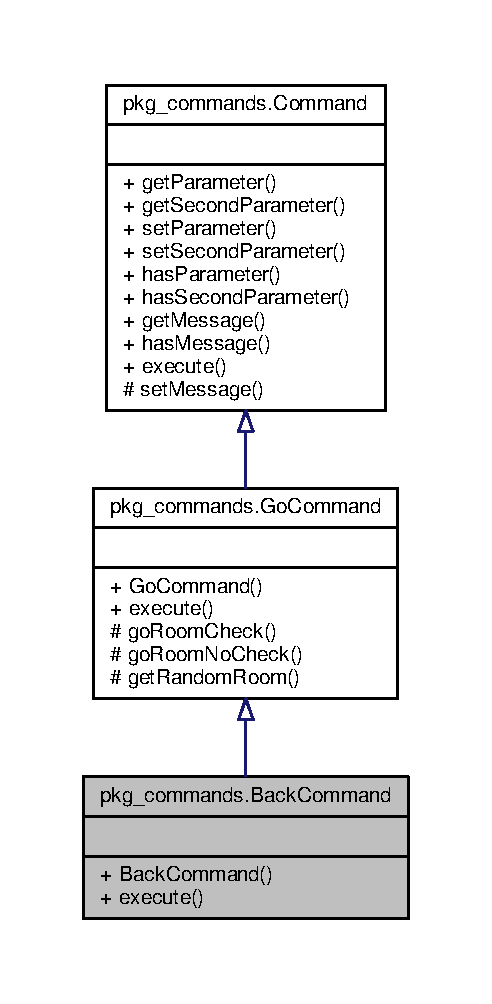
\includegraphics[width=236pt]{classpkg__commands_1_1BackCommand__inherit__graph}
\end{center}
\end{figure}


Collaboration diagram for pkg\-\_\-commands.\-Back\-Command\-:
\nopagebreak
\begin{figure}[H]
\begin{center}
\leavevmode
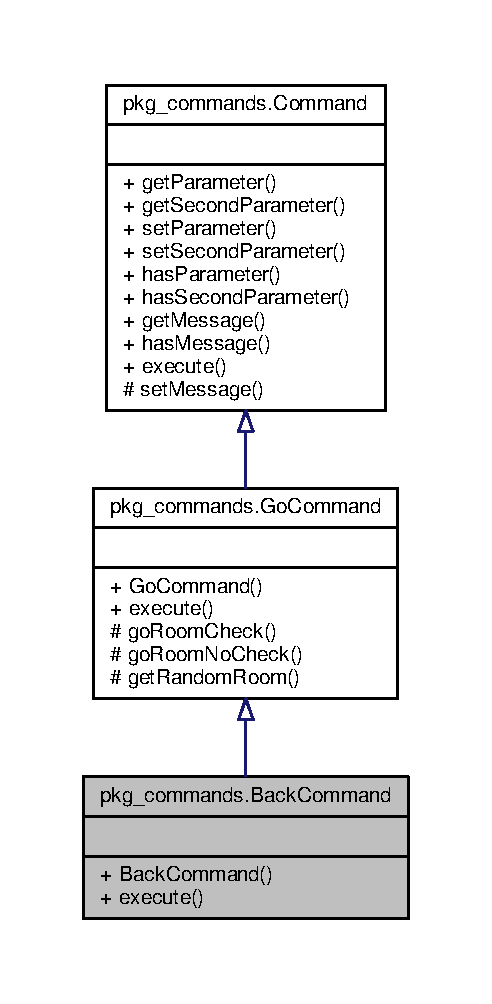
\includegraphics[width=236pt]{classpkg__commands_1_1BackCommand__coll__graph}
\end{center}
\end{figure}
\subsection*{Public Member Functions}
\begin{DoxyCompactItemize}
\item 
\hyperlink{classpkg__commands_1_1BackCommand_a81518eb89a9e9126e51f2f7ba6ff1ed9}{Back\-Command} ()
\item 
boolean \hyperlink{classpkg__commands_1_1BackCommand_a35bf0276436a619d7baeb9c3a752f9d6}{execute} (\hyperlink{classpkg__world_1_1Player}{Player} player)  throws Unauthorized\-Exception 
\end{DoxyCompactItemize}
\subsection*{Additional Inherited Members}


\subsection{Detailed Description}
class \hyperlink{classpkg__commands_1_1BackCommand}{Back\-Command} used to go back in a previous Room. \begin{DoxyAuthor}{Author}
Rémi N\-I\-C\-O\-L\-E 
\end{DoxyAuthor}


Definition at line \hyperlink{BackCommand_8java_source_l00010}{10} of file \hyperlink{BackCommand_8java_source}{Back\-Command.\-java}.



\subsection{Constructor \& Destructor Documentation}
\hypertarget{classpkg__commands_1_1BackCommand_a81518eb89a9e9126e51f2f7ba6ff1ed9}{\index{pkg\-\_\-commands\-::\-Back\-Command@{pkg\-\_\-commands\-::\-Back\-Command}!Back\-Command@{Back\-Command}}
\index{Back\-Command@{Back\-Command}!pkg_commands::BackCommand@{pkg\-\_\-commands\-::\-Back\-Command}}
\subsubsection[{Back\-Command}]{\setlength{\rightskip}{0pt plus 5cm}pkg\-\_\-commands.\-Back\-Command.\-Back\-Command (
\begin{DoxyParamCaption}
{}
\end{DoxyParamCaption}
)}}\label{classpkg__commands_1_1BackCommand_a81518eb89a9e9126e51f2f7ba6ff1ed9}
Constructor for \hyperlink{classpkg__commands_1_1BackCommand}{Back\-Command} 

Definition at line \hyperlink{BackCommand_8java_source_l00015}{15} of file \hyperlink{BackCommand_8java_source}{Back\-Command.\-java}.


\begin{DoxyCode}
00015                         \{
00016         super();
00017     \}
\end{DoxyCode}


\subsection{Member Function Documentation}
\hypertarget{classpkg__commands_1_1BackCommand_a35bf0276436a619d7baeb9c3a752f9d6}{\index{pkg\-\_\-commands\-::\-Back\-Command@{pkg\-\_\-commands\-::\-Back\-Command}!execute@{execute}}
\index{execute@{execute}!pkg_commands::BackCommand@{pkg\-\_\-commands\-::\-Back\-Command}}
\subsubsection[{execute}]{\setlength{\rightskip}{0pt plus 5cm}boolean pkg\-\_\-commands.\-Back\-Command.\-execute (
\begin{DoxyParamCaption}
\item[{{\bf Player}}]{player}
\end{DoxyParamCaption}
) throws {\bf Unauthorized\-Exception}}}\label{classpkg__commands_1_1BackCommand_a35bf0276436a619d7baeb9c3a752f9d6}
Go back in a previous room of the player. 
\begin{DoxyParams}{Parameters}
{\em player} & The player that typed the \char`\"{}back\char`\"{} command \\
\hline
\end{DoxyParams}

\begin{DoxyExceptions}{Exceptions}
{\em Unauthorized\-Exception} & When the user has no previous room \\
\hline
\end{DoxyExceptions}
\begin{DoxyReturn}{Returns}
False because it is not the quit command 
\end{DoxyReturn}


Definition at line \hyperlink{BackCommand_8java_source_l00025}{25} of file \hyperlink{BackCommand_8java_source}{Back\-Command.\-java}.


\begin{DoxyCode}
00025                                                                        \{
00026         \textcolor{keywordflow}{try} \{
00027             super.goRoomCheck(player.getPreviousRoom(), player, \textcolor{keyword}{true});
00028         \} \textcolor{keywordflow}{catch}(pkg\_exceptions.IllegalArgumentException e)  \{
00029             \textcolor{comment}{// Tried to teleport to null}
00030             \textcolor{keywordflow}{throw} \textcolor{keyword}{new} UnauthorizedException(\textcolor{stringliteral}{"Awww, that's sweet. The little player want to go home.\(\backslash\)n"}
00031                     + \textcolor{stringliteral}{"But we're just getting started!"});
00032         \}
00033         \textcolor{keywordflow}{return} \textcolor{keyword}{false};
00034     \}
\end{DoxyCode}


The documentation for this class was generated from the following file\-:\begin{DoxyCompactItemize}
\item 
pkg\-\_\-commands/\hyperlink{BackCommand_8java}{Back\-Command.\-java}\end{DoxyCompactItemize}

\hypertarget{classpkg__commands_1_1BeamerCommand}{\section{pkg\-\_\-commands.\-Beamer\-Command Class Reference}
\label{classpkg__commands_1_1BeamerCommand}\index{pkg\-\_\-commands.\-Beamer\-Command@{pkg\-\_\-commands.\-Beamer\-Command}}
}


class \hyperlink{classpkg__commands_1_1BeamerCommand}{Beamer\-Command} used to teleport into a remembered room  




Inheritance diagram for pkg\-\_\-commands.\-Beamer\-Command\-:
\nopagebreak
\begin{figure}[H]
\begin{center}
\leavevmode
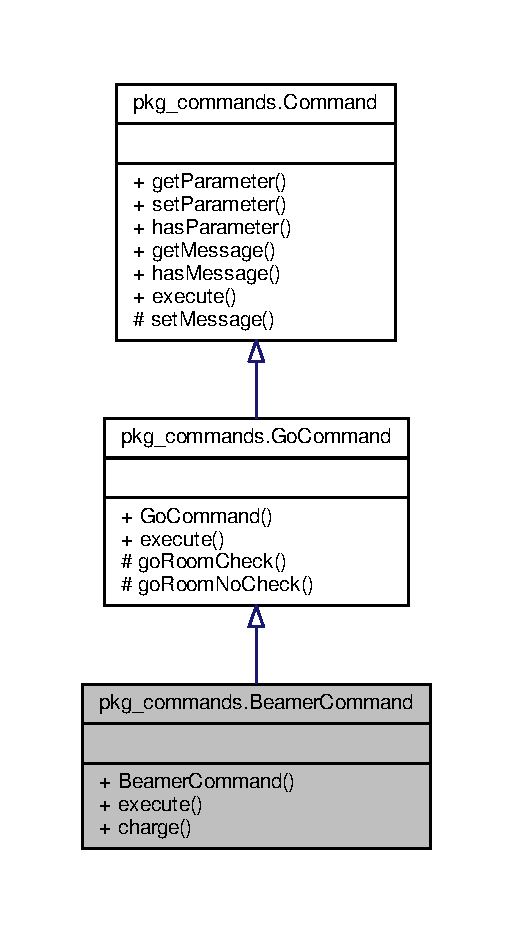
\includegraphics[width=246pt]{classpkg__commands_1_1BeamerCommand__inherit__graph}
\end{center}
\end{figure}


Collaboration diagram for pkg\-\_\-commands.\-Beamer\-Command\-:
\nopagebreak
\begin{figure}[H]
\begin{center}
\leavevmode
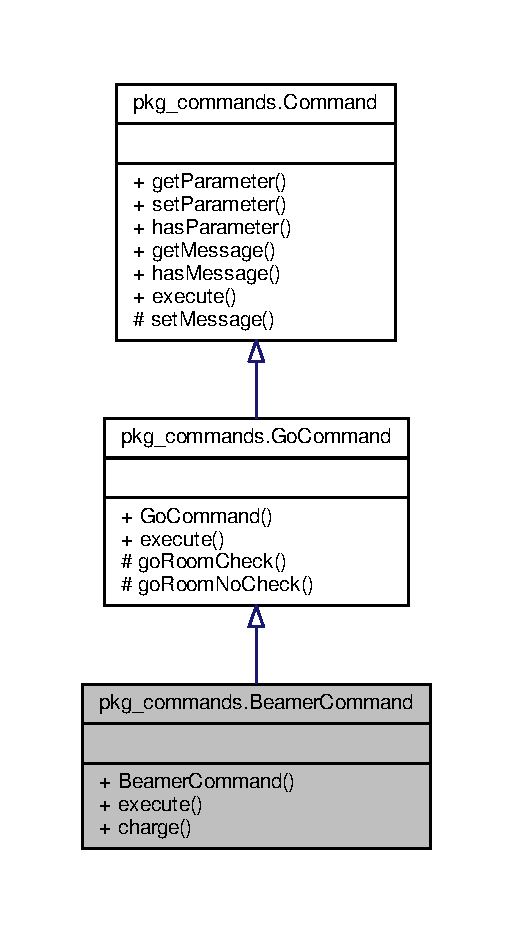
\includegraphics[width=246pt]{classpkg__commands_1_1BeamerCommand__coll__graph}
\end{center}
\end{figure}
\subsection*{Public Member Functions}
\begin{DoxyCompactItemize}
\item 
\hyperlink{classpkg__commands_1_1BeamerCommand_a541cd046e7680452f451322c1730e675}{Beamer\-Command} ()
\begin{DoxyCompactList}\small\item\em Constructor for \hyperlink{classpkg__commands_1_1BeamerCommand}{Beamer\-Command}. \end{DoxyCompactList}\item 
boolean \hyperlink{classpkg__commands_1_1BeamerCommand_a139dc852e180cabd8af15cfed37dcf0e}{execute} (\hyperlink{classpkg__world_1_1Player}{Player} player)  throws No\-Argument\-Exception,pkg\-\_\-exceptions.\-Illegal\-Argument\-Exception,\-Unauthorized\-Exception 
\begin{DoxyCompactList}\small\item\em Teleport to the remembered room or remember a room. \end{DoxyCompactList}\item 
void \hyperlink{classpkg__commands_1_1BeamerCommand_ae71665296a18d581ad1f714c1078e37b}{charge} (\hyperlink{classpkg__world_1_1Player}{Player} player)
\begin{DoxyCompactList}\small\item\em Remember the current room. \end{DoxyCompactList}\end{DoxyCompactItemize}
\subsection*{Additional Inherited Members}


\subsection{Detailed Description}
class \hyperlink{classpkg__commands_1_1BeamerCommand}{Beamer\-Command} used to teleport into a remembered room 

\begin{DoxyAuthor}{Author}
Rémi N\-I\-C\-O\-L\-E 
\end{DoxyAuthor}


Definition at line \hyperlink{BeamerCommand_8java_source_l00010}{10} of file \hyperlink{BeamerCommand_8java_source}{Beamer\-Command.\-java}.



\subsection{Constructor \& Destructor Documentation}
\hypertarget{classpkg__commands_1_1BeamerCommand_a541cd046e7680452f451322c1730e675}{\index{pkg\-\_\-commands\-::\-Beamer\-Command@{pkg\-\_\-commands\-::\-Beamer\-Command}!Beamer\-Command@{Beamer\-Command}}
\index{Beamer\-Command@{Beamer\-Command}!pkg_commands::BeamerCommand@{pkg\-\_\-commands\-::\-Beamer\-Command}}
\subsubsection[{Beamer\-Command}]{\setlength{\rightskip}{0pt plus 5cm}pkg\-\_\-commands.\-Beamer\-Command.\-Beamer\-Command (
\begin{DoxyParamCaption}
{}
\end{DoxyParamCaption}
)}}\label{classpkg__commands_1_1BeamerCommand_a541cd046e7680452f451322c1730e675}


Constructor for \hyperlink{classpkg__commands_1_1BeamerCommand}{Beamer\-Command}. 



Definition at line \hyperlink{BeamerCommand_8java_source_l00015}{15} of file \hyperlink{BeamerCommand_8java_source}{Beamer\-Command.\-java}.


\begin{DoxyCode}
00015                           \{
00016 
00017     \}
\end{DoxyCode}


\subsection{Member Function Documentation}
\hypertarget{classpkg__commands_1_1BeamerCommand_ae71665296a18d581ad1f714c1078e37b}{\index{pkg\-\_\-commands\-::\-Beamer\-Command@{pkg\-\_\-commands\-::\-Beamer\-Command}!charge@{charge}}
\index{charge@{charge}!pkg_commands::BeamerCommand@{pkg\-\_\-commands\-::\-Beamer\-Command}}
\subsubsection[{charge}]{\setlength{\rightskip}{0pt plus 5cm}void pkg\-\_\-commands.\-Beamer\-Command.\-charge (
\begin{DoxyParamCaption}
\item[{{\bf Player}}]{player}
\end{DoxyParamCaption}
)}}\label{classpkg__commands_1_1BeamerCommand_ae71665296a18d581ad1f714c1078e37b}


Remember the current room. 


\begin{DoxyParams}{Parameters}
{\em player} & The player that called this command \\
\hline
\end{DoxyParams}


Definition at line \hyperlink{BeamerCommand_8java_source_l00067}{67} of file \hyperlink{BeamerCommand_8java_source}{Beamer\-Command.\-java}.



References \hyperlink{Player_8java_source_l00167}{pkg\-\_\-world.\-Player.\-get\-Beamer\-Room()}, and \hyperlink{Command_8java_source_l00089}{pkg\-\_\-commands.\-Command.\-set\-Message()}.



Referenced by \hyperlink{BeamerCommand_8java_source_l00030}{pkg\-\_\-commands.\-Beamer\-Command.\-execute()}.


\begin{DoxyCode}
00067                                       \{
00068         \textcolor{keywordflow}{if}(player.getBeamerRoom() == null)
00069             \hyperlink{classpkg__commands_1_1Command_ae210ff216fe908b111ba1c988a963d13}{setMessage}(\textcolor{stringliteral}{"Useless room remembered."});
00070         \textcolor{keywordflow}{else}
00071             \hyperlink{classpkg__commands_1_1Command_ae210ff216fe908b111ba1c988a963d13}{setMessage}(\textcolor{stringliteral}{"Useful room overridden by a useless room."});
00072         player.setBeamerRoom(player.getCurrentRoom());
00073     \}
\end{DoxyCode}


Here is the call graph for this function\-:
\nopagebreak
\begin{figure}[H]
\begin{center}
\leavevmode
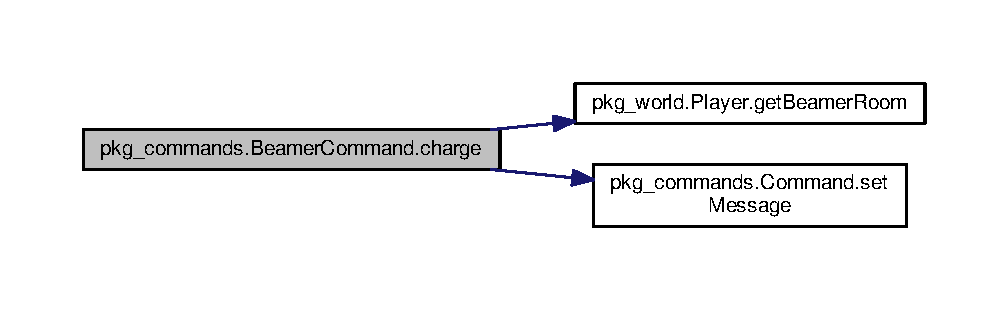
\includegraphics[width=350pt]{classpkg__commands_1_1BeamerCommand_ae71665296a18d581ad1f714c1078e37b_cgraph}
\end{center}
\end{figure}




Here is the caller graph for this function\-:
\nopagebreak
\begin{figure}[H]
\begin{center}
\leavevmode
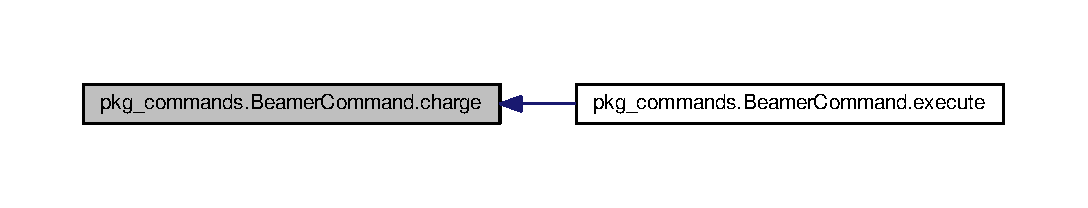
\includegraphics[width=350pt]{classpkg__commands_1_1BeamerCommand_ae71665296a18d581ad1f714c1078e37b_icgraph}
\end{center}
\end{figure}


\hypertarget{classpkg__commands_1_1BeamerCommand_a139dc852e180cabd8af15cfed37dcf0e}{\index{pkg\-\_\-commands\-::\-Beamer\-Command@{pkg\-\_\-commands\-::\-Beamer\-Command}!execute@{execute}}
\index{execute@{execute}!pkg_commands::BeamerCommand@{pkg\-\_\-commands\-::\-Beamer\-Command}}
\subsubsection[{execute}]{\setlength{\rightskip}{0pt plus 5cm}boolean pkg\-\_\-commands.\-Beamer\-Command.\-execute (
\begin{DoxyParamCaption}
\item[{{\bf Player}}]{player}
\end{DoxyParamCaption}
) throws {\bf No\-Argument\-Exception},{\bf pkg\-\_\-exceptions.\-Illegal\-Argument\-Exception},{\bf Unauthorized\-Exception}}}\label{classpkg__commands_1_1BeamerCommand_a139dc852e180cabd8af15cfed37dcf0e}


Teleport to the remembered room or remember a room. 

It teleports to the remembered room if the command parameter was \char`\"{}teleport\char`\"{}, and it remembers the room if the command parameter was \char`\"{}charge\char`\"{} 
\begin{DoxyParams}{Parameters}
{\em player} & The player that called this command \\
\hline
\end{DoxyParams}

\begin{DoxyExceptions}{Exceptions}
{\em No\-Argument\-Exception} & When the user typed the command without parameter \\
\hline
{\em Illegal\-Argument\-Exception} & When the user typed a parameter other than \char`\"{}teleport\char`\"{} or \char`\"{}charge\char`\"{} \\
\hline
{\em Unauthorized\-Exception} & When the user tries to teleport to null \\
\hline
\end{DoxyExceptions}
\begin{DoxyReturn}{Returns}
False because it is not the quit command 
\end{DoxyReturn}


Definition at line \hyperlink{BeamerCommand_8java_source_l00030}{30} of file \hyperlink{BeamerCommand_8java_source}{Beamer\-Command.\-java}.



References \hyperlink{BeamerCommand_8java_source_l00067}{pkg\-\_\-commands.\-Beamer\-Command.\-charge()}, \hyperlink{Command_8java_source_l00041}{pkg\-\_\-commands.\-Command.\-get\-Parameter()}, and \hyperlink{Command_8java_source_l00073}{pkg\-\_\-commands.\-Command.\-has\-Parameter()}.


\begin{DoxyCode}
00030                                                                                                            
                              \{
00031         \textcolor{keywordflow}{if}(\hyperlink{classpkg__commands_1_1Command_a02af95ab3f1898a66259ab7c177b6998}{hasParameter}()) \{
00032             \textcolor{keywordflow}{if}(\hyperlink{classpkg__commands_1_1Command_a41c92d445be73ea9d62320c65efb8434}{getParameter}().equals(\textcolor{stringliteral}{"charge"})) \{
00033                 \hyperlink{classpkg__commands_1_1BeamerCommand_ae71665296a18d581ad1f714c1078e37b}{charge}(player);
00034                 \textcolor{keywordflow}{return} \textcolor{keyword}{false};
00035             \} \textcolor{keywordflow}{else} \textcolor{keywordflow}{if}(\hyperlink{classpkg__commands_1_1Command_a41c92d445be73ea9d62320c65efb8434}{getParameter}().equals(\textcolor{stringliteral}{"teleport"})) \{
00036                 teleport(player);
00037                 \textcolor{keywordflow}{return} \textcolor{keyword}{false};
00038             \} \textcolor{keywordflow}{else} \{
00039                 \textcolor{keywordflow}{throw} \textcolor{keyword}{new} \hyperlink{classpkg__exceptions_1_1IllegalArgumentException}{pkg\_exceptions.IllegalArgumentException}(\textcolor{stringliteral}{"
      In order to do that, I may need to upgrade. But I don't want to."});
00040             \}
00041         \} \textcolor{keywordflow}{else} 
00042             \textcolor{keywordflow}{throw} \textcolor{keyword}{new} \hyperlink{classpkg__exceptions_1_1NoArgumentException}{NoArgumentException}(\textcolor{stringliteral}{"You can either charge or teleport with the
       beamer.\(\backslash\)nBut that may be too much complicated for you, isn't it?"});
00043     \}
\end{DoxyCode}


Here is the call graph for this function\-:
\nopagebreak
\begin{figure}[H]
\begin{center}
\leavevmode
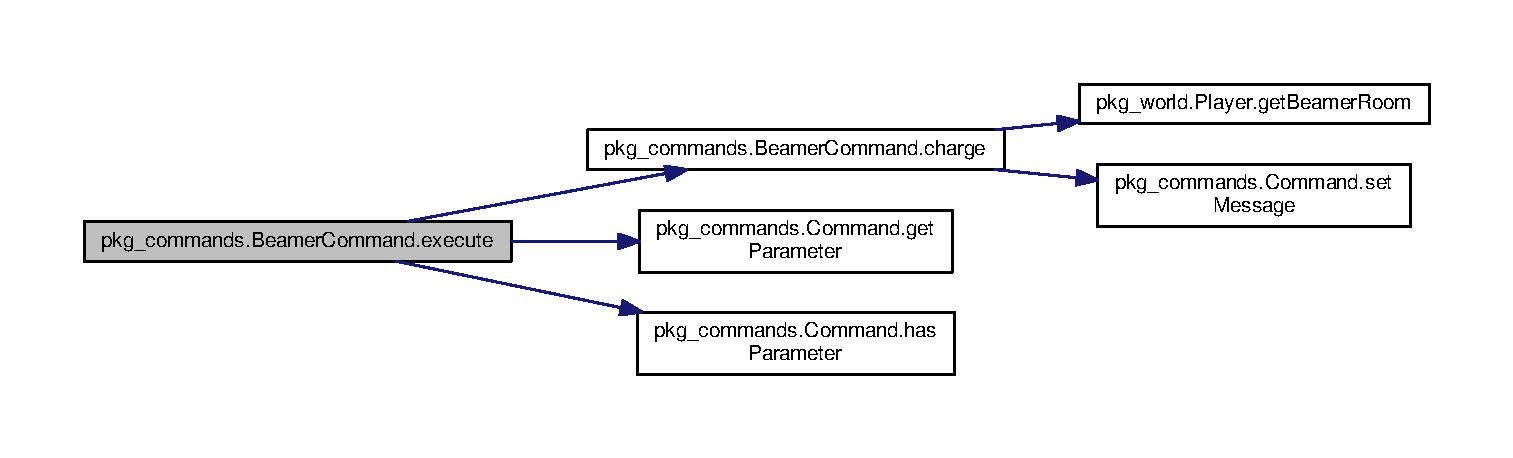
\includegraphics[width=350pt]{classpkg__commands_1_1BeamerCommand_a139dc852e180cabd8af15cfed37dcf0e_cgraph}
\end{center}
\end{figure}




The documentation for this class was generated from the following file\-:\begin{DoxyCompactItemize}
\item 
pkg\-\_\-commands/\hyperlink{BeamerCommand_8java}{Beamer\-Command.\-java}\end{DoxyCompactItemize}

\hypertarget{classpkg__commands_1_1Command}{\section{pkg\-\_\-commands.\-Command Class Reference}
\label{classpkg__commands_1_1Command}\index{pkg\-\_\-commands.\-Command@{pkg\-\_\-commands.\-Command}}
}


Class used to handle a command of one or two words.  




Inheritance diagram for pkg\-\_\-commands.\-Command\-:
\nopagebreak
\begin{figure}[H]
\begin{center}
\leavevmode
\includegraphics[width=350pt]{classpkg__commands_1_1Command__inherit__graph}
\end{center}
\end{figure}


Collaboration diagram for pkg\-\_\-commands.\-Command\-:
\nopagebreak
\begin{figure}[H]
\begin{center}
\leavevmode
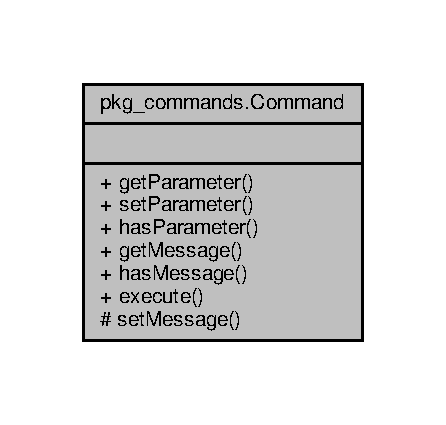
\includegraphics[width=214pt]{classpkg__commands_1_1Command__coll__graph}
\end{center}
\end{figure}
\subsection*{Public Member Functions}
\begin{DoxyCompactItemize}
\item 
String \hyperlink{classpkg__commands_1_1Command_a41c92d445be73ea9d62320c65efb8434}{get\-Parameter} ()
\begin{DoxyCompactList}\small\item\em Parameter field getter. \end{DoxyCompactList}\item 
String \hyperlink{classpkg__commands_1_1Command_a20d3ebdc0683a87b43be2a92a1cad111}{get\-Second\-Parameter} ()
\begin{DoxyCompactList}\small\item\em Second Parameter field getter. \end{DoxyCompactList}\item 
void \hyperlink{classpkg__commands_1_1Command_a18446243a5fd360e9341b4b141c0cccc}{set\-Parameter} (String parameter)
\begin{DoxyCompactList}\small\item\em Parameter field setter. \end{DoxyCompactList}\item 
void \hyperlink{classpkg__commands_1_1Command_af6de3828c27cd491ad24c4a97d69e856}{set\-Second\-Parameter} (String parameter)
\begin{DoxyCompactList}\small\item\em Second Parameter field setter. \end{DoxyCompactList}\item 
boolean \hyperlink{classpkg__commands_1_1Command_a02af95ab3f1898a66259ab7c177b6998}{has\-Parameter} ()
\begin{DoxyCompactList}\small\item\em Return true if the parameter is null. \end{DoxyCompactList}\item 
boolean \hyperlink{classpkg__commands_1_1Command_add688a76d80576c34f23927da19b9e2d}{has\-Second\-Parameter} ()
\begin{DoxyCompactList}\small\item\em Return true if the second parameter is null. \end{DoxyCompactList}\item 
String \hyperlink{classpkg__commands_1_1Command_ac2a42e2bab264821892daefaf9a18b6c}{get\-Message} ()
\begin{DoxyCompactList}\small\item\em Message field getter. \end{DoxyCompactList}\item 
boolean \hyperlink{classpkg__commands_1_1Command_ae46bb048d0fa705a5037a5204b530da2}{has\-Message} ()
\begin{DoxyCompactList}\small\item\em Return true if the message is equal to null or \char`\"{}\char`\"{}. \end{DoxyCompactList}\item 
abstract boolean \hyperlink{classpkg__commands_1_1Command_a19008923c75a87c87d1f3ba8bf8be43f}{execute} (\hyperlink{classpkg__world_1_1Player}{Player} player)  throws No\-Argument\-Exception,pkg\-\_\-exceptions.\-Illegal\-Argument\-Exception,\-Unauthorized\-Exception
\begin{DoxyCompactList}\small\item\em Process the command. \end{DoxyCompactList}\end{DoxyCompactItemize}
\subsection*{Protected Member Functions}
\begin{DoxyCompactItemize}
\item 
void \hyperlink{classpkg__commands_1_1Command_ae210ff216fe908b111ba1c988a963d13}{set\-Message} (String message)
\begin{DoxyCompactList}\small\item\em Message field setter. \end{DoxyCompactList}\end{DoxyCompactItemize}


\subsection{Detailed Description}
Class used to handle a command of one or two words. 

\begin{DoxyAuthor}{Author}
Rémi N\-I\-C\-O\-L\-E 
\end{DoxyAuthor}


Definition at line \hyperlink{Command_8java_source_l00014}{14} of file \hyperlink{Command_8java_source}{Command.\-java}.



\subsection{Member Function Documentation}
\hypertarget{classpkg__commands_1_1Command_a19008923c75a87c87d1f3ba8bf8be43f}{\index{pkg\-\_\-commands\-::\-Command@{pkg\-\_\-commands\-::\-Command}!execute@{execute}}
\index{execute@{execute}!pkg_commands::Command@{pkg\-\_\-commands\-::\-Command}}
\subsubsection[{execute}]{\setlength{\rightskip}{0pt plus 5cm}abstract boolean pkg\-\_\-commands.\-Command.\-execute (
\begin{DoxyParamCaption}
\item[{{\bf Player}}]{player}
\end{DoxyParamCaption}
) throws {\bf No\-Argument\-Exception},{\bf pkg\-\_\-exceptions.\-Illegal\-Argument\-Exception},{\bf Unauthorized\-Exception}\hspace{0.3cm}{\ttfamily [abstract]}}}\label{classpkg__commands_1_1Command_a19008923c75a87c87d1f3ba8bf8be43f}


Process the command. 


\begin{DoxyParams}{Parameters}
{\em player} & The player that called this command \\
\hline
\end{DoxyParams}

\begin{DoxyExceptions}{Exceptions}
{\em No\-Argument\-Exception} & When the command needed a parameter but the user didn't specify one \\
\hline
{\em Illegal\-Argument\-Exception} & When the user typed a parameter other than the correct ones \\
\hline
{\em Unauthorized\-Exception} & When the user isn't allowed to do this action \\
\hline
\end{DoxyExceptions}
\hypertarget{classpkg__commands_1_1Command_ac2a42e2bab264821892daefaf9a18b6c}{\index{pkg\-\_\-commands\-::\-Command@{pkg\-\_\-commands\-::\-Command}!get\-Message@{get\-Message}}
\index{get\-Message@{get\-Message}!pkg_commands::Command@{pkg\-\_\-commands\-::\-Command}}
\subsubsection[{get\-Message}]{\setlength{\rightskip}{0pt plus 5cm}String pkg\-\_\-commands.\-Command.\-get\-Message (
\begin{DoxyParamCaption}
{}
\end{DoxyParamCaption}
)}}\label{classpkg__commands_1_1Command_ac2a42e2bab264821892daefaf9a18b6c}


Message field getter. 

\begin{DoxyReturn}{Returns}
The message to print to the user 
\end{DoxyReturn}


Definition at line \hyperlink{Command_8java_source_l00097}{97} of file \hyperlink{Command_8java_source}{Command.\-java}.



Referenced by \hyperlink{TestCommand_8java_source_l00032}{pkg\-\_\-commands.\-Test\-Command.\-execute()}, \hyperlink{HelpCommand_8java_source_l00033}{pkg\-\_\-commands.\-Help\-Command.\-execute()}, and \hyperlink{GoCommand_8java_source_l00071}{pkg\-\_\-commands.\-Go\-Command.\-go\-Room\-No\-Check()}.


\begin{DoxyCode}
00097                                \{
00098         \textcolor{keywordflow}{return} (message == null)? \textcolor{stringliteral}{""} : message;
00099     \}
\end{DoxyCode}


Here is the caller graph for this function\-:
\nopagebreak
\begin{figure}[H]
\begin{center}
\leavevmode
\includegraphics[width=350pt]{classpkg__commands_1_1Command_ac2a42e2bab264821892daefaf9a18b6c_icgraph}
\end{center}
\end{figure}


\hypertarget{classpkg__commands_1_1Command_a41c92d445be73ea9d62320c65efb8434}{\index{pkg\-\_\-commands\-::\-Command@{pkg\-\_\-commands\-::\-Command}!get\-Parameter@{get\-Parameter}}
\index{get\-Parameter@{get\-Parameter}!pkg_commands::Command@{pkg\-\_\-commands\-::\-Command}}
\subsubsection[{get\-Parameter}]{\setlength{\rightskip}{0pt plus 5cm}String pkg\-\_\-commands.\-Command.\-get\-Parameter (
\begin{DoxyParamCaption}
{}
\end{DoxyParamCaption}
)}}\label{classpkg__commands_1_1Command_a41c92d445be73ea9d62320c65efb8434}


Parameter field getter. 

\begin{DoxyReturn}{Returns}
The parameter given by the user 
\end{DoxyReturn}


Definition at line \hyperlink{Command_8java_source_l00041}{41} of file \hyperlink{Command_8java_source}{Command.\-java}.



Referenced by \hyperlink{LookCommand_8java_source_l00026}{pkg\-\_\-commands.\-Look\-Command.\-execute()}, \hyperlink{TalkCommand_8java_source_l00027}{pkg\-\_\-commands.\-Talk\-Command.\-execute()}, \hyperlink{DropCommand_8java_source_l00027}{pkg\-\_\-commands.\-Drop\-Command.\-execute()}, \hyperlink{TakeCommand_8java_source_l00027}{pkg\-\_\-commands.\-Take\-Command.\-execute()}, \hyperlink{ThrowCommand_8java_source_l00028}{pkg\-\_\-commands.\-Throw\-Command.\-execute()}, \hyperlink{EatCommand_8java_source_l00028}{pkg\-\_\-commands.\-Eat\-Command.\-execute()}, \hyperlink{GiveCommand_8java_source_l00029}{pkg\-\_\-commands.\-Give\-Command.\-execute()}, \hyperlink{BeamerCommand_8java_source_l00030}{pkg\-\_\-commands.\-Beamer\-Command.\-execute()}, \hyperlink{TestCommand_8java_source_l00032}{pkg\-\_\-commands.\-Test\-Command.\-execute()}, and \hyperlink{GoCommand_8java_source_l00032}{pkg\-\_\-commands.\-Go\-Command.\-execute()}.


\begin{DoxyCode}
00041                                  \{
00042         \textcolor{keywordflow}{return} parameter;
00043     \}
\end{DoxyCode}


Here is the caller graph for this function\-:
\nopagebreak
\begin{figure}[H]
\begin{center}
\leavevmode
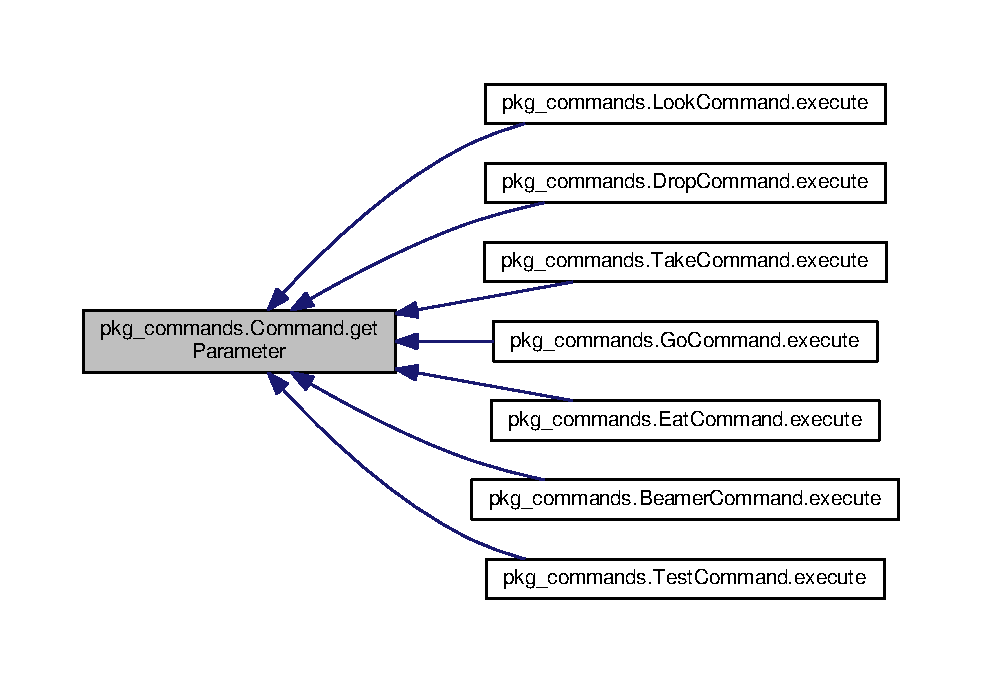
\includegraphics[width=350pt]{classpkg__commands_1_1Command_a41c92d445be73ea9d62320c65efb8434_icgraph}
\end{center}
\end{figure}


\hypertarget{classpkg__commands_1_1Command_a20d3ebdc0683a87b43be2a92a1cad111}{\index{pkg\-\_\-commands\-::\-Command@{pkg\-\_\-commands\-::\-Command}!get\-Second\-Parameter@{get\-Second\-Parameter}}
\index{get\-Second\-Parameter@{get\-Second\-Parameter}!pkg_commands::Command@{pkg\-\_\-commands\-::\-Command}}
\subsubsection[{get\-Second\-Parameter}]{\setlength{\rightskip}{0pt plus 5cm}String pkg\-\_\-commands.\-Command.\-get\-Second\-Parameter (
\begin{DoxyParamCaption}
{}
\end{DoxyParamCaption}
)}}\label{classpkg__commands_1_1Command_a20d3ebdc0683a87b43be2a92a1cad111}


Second Parameter field getter. 

\begin{DoxyReturn}{Returns}
The second parameter given by the user 
\end{DoxyReturn}


Definition at line \hyperlink{Command_8java_source_l00049}{49} of file \hyperlink{Command_8java_source}{Command.\-java}.



Referenced by \hyperlink{GiveCommand_8java_source_l00029}{pkg\-\_\-commands.\-Give\-Command.\-execute()}.


\begin{DoxyCode}
00049                                        \{
00050         \textcolor{keywordflow}{return} secondParameter;
00051     \}
\end{DoxyCode}


Here is the caller graph for this function\-:
\nopagebreak
\begin{figure}[H]
\begin{center}
\leavevmode
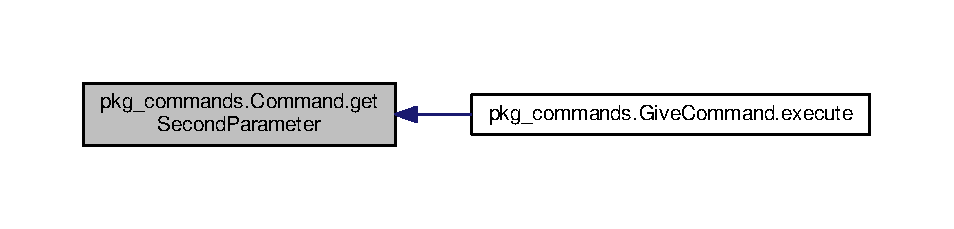
\includegraphics[width=350pt]{classpkg__commands_1_1Command_a20d3ebdc0683a87b43be2a92a1cad111_icgraph}
\end{center}
\end{figure}


\hypertarget{classpkg__commands_1_1Command_ae46bb048d0fa705a5037a5204b530da2}{\index{pkg\-\_\-commands\-::\-Command@{pkg\-\_\-commands\-::\-Command}!has\-Message@{has\-Message}}
\index{has\-Message@{has\-Message}!pkg_commands::Command@{pkg\-\_\-commands\-::\-Command}}
\subsubsection[{has\-Message}]{\setlength{\rightskip}{0pt plus 5cm}boolean pkg\-\_\-commands.\-Command.\-has\-Message (
\begin{DoxyParamCaption}
{}
\end{DoxyParamCaption}
)}}\label{classpkg__commands_1_1Command_ae46bb048d0fa705a5037a5204b530da2}


Return true if the message is equal to null or \char`\"{}\char`\"{}. 

\begin{DoxyReturn}{Returns}
True if the message is equal to null or \char`\"{}\char`\"{} 
\end{DoxyReturn}


Definition at line \hyperlink{Command_8java_source_l00105}{105} of file \hyperlink{Command_8java_source}{Command.\-java}.



Referenced by \hyperlink{GoCommand_8java_source_l00071}{pkg\-\_\-commands.\-Go\-Command.\-go\-Room\-No\-Check()}.


\begin{DoxyCode}
00105                                 \{
00106         \textcolor{keywordflow}{return} (message == null) ? \textcolor{keyword}{false} : !message.equals(\textcolor{stringliteral}{""});
00107     \}
\end{DoxyCode}


Here is the caller graph for this function\-:
\nopagebreak
\begin{figure}[H]
\begin{center}
\leavevmode
\includegraphics[width=350pt]{classpkg__commands_1_1Command_ae46bb048d0fa705a5037a5204b530da2_icgraph}
\end{center}
\end{figure}


\hypertarget{classpkg__commands_1_1Command_a02af95ab3f1898a66259ab7c177b6998}{\index{pkg\-\_\-commands\-::\-Command@{pkg\-\_\-commands\-::\-Command}!has\-Parameter@{has\-Parameter}}
\index{has\-Parameter@{has\-Parameter}!pkg_commands::Command@{pkg\-\_\-commands\-::\-Command}}
\subsubsection[{has\-Parameter}]{\setlength{\rightskip}{0pt plus 5cm}boolean pkg\-\_\-commands.\-Command.\-has\-Parameter (
\begin{DoxyParamCaption}
{}
\end{DoxyParamCaption}
)}}\label{classpkg__commands_1_1Command_a02af95ab3f1898a66259ab7c177b6998}


Return true if the parameter is null. 

\begin{DoxyReturn}{Returns}
True if the parameter is null 
\end{DoxyReturn}


Definition at line \hyperlink{Command_8java_source_l00073}{73} of file \hyperlink{Command_8java_source}{Command.\-java}.



Referenced by \hyperlink{LookCommand_8java_source_l00026}{pkg\-\_\-commands.\-Look\-Command.\-execute()}, \hyperlink{TalkCommand_8java_source_l00027}{pkg\-\_\-commands.\-Talk\-Command.\-execute()}, \hyperlink{DropCommand_8java_source_l00027}{pkg\-\_\-commands.\-Drop\-Command.\-execute()}, \hyperlink{TakeCommand_8java_source_l00027}{pkg\-\_\-commands.\-Take\-Command.\-execute()}, \hyperlink{ThrowCommand_8java_source_l00028}{pkg\-\_\-commands.\-Throw\-Command.\-execute()}, \hyperlink{EatCommand_8java_source_l00028}{pkg\-\_\-commands.\-Eat\-Command.\-execute()}, \hyperlink{GiveCommand_8java_source_l00029}{pkg\-\_\-commands.\-Give\-Command.\-execute()}, \hyperlink{BeamerCommand_8java_source_l00030}{pkg\-\_\-commands.\-Beamer\-Command.\-execute()}, \hyperlink{TestCommand_8java_source_l00032}{pkg\-\_\-commands.\-Test\-Command.\-execute()}, and \hyperlink{GoCommand_8java_source_l00032}{pkg\-\_\-commands.\-Go\-Command.\-execute()}.


\begin{DoxyCode}
00073                                   \{
00074         \textcolor{keywordflow}{return} (parameter != null);
00075     \}
\end{DoxyCode}


Here is the caller graph for this function\-:
\nopagebreak
\begin{figure}[H]
\begin{center}
\leavevmode
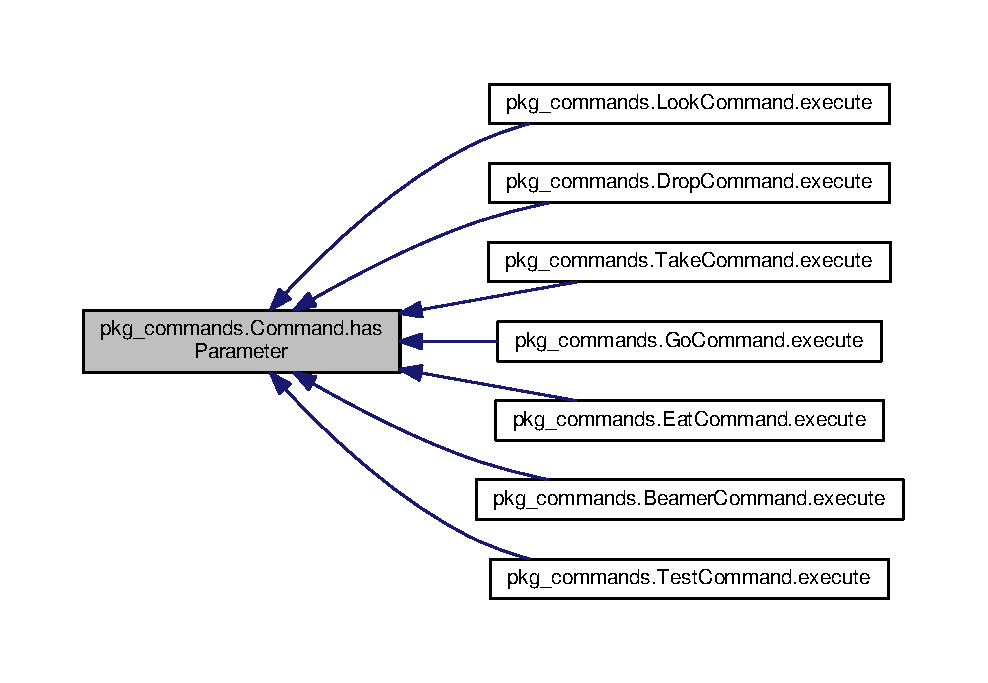
\includegraphics[width=350pt]{classpkg__commands_1_1Command_a02af95ab3f1898a66259ab7c177b6998_icgraph}
\end{center}
\end{figure}


\hypertarget{classpkg__commands_1_1Command_add688a76d80576c34f23927da19b9e2d}{\index{pkg\-\_\-commands\-::\-Command@{pkg\-\_\-commands\-::\-Command}!has\-Second\-Parameter@{has\-Second\-Parameter}}
\index{has\-Second\-Parameter@{has\-Second\-Parameter}!pkg_commands::Command@{pkg\-\_\-commands\-::\-Command}}
\subsubsection[{has\-Second\-Parameter}]{\setlength{\rightskip}{0pt plus 5cm}boolean pkg\-\_\-commands.\-Command.\-has\-Second\-Parameter (
\begin{DoxyParamCaption}
{}
\end{DoxyParamCaption}
)}}\label{classpkg__commands_1_1Command_add688a76d80576c34f23927da19b9e2d}


Return true if the second parameter is null. 

\begin{DoxyReturn}{Returns}
True if the second parameter is null 
\end{DoxyReturn}


Definition at line \hyperlink{Command_8java_source_l00081}{81} of file \hyperlink{Command_8java_source}{Command.\-java}.



Referenced by \hyperlink{GiveCommand_8java_source_l00029}{pkg\-\_\-commands.\-Give\-Command.\-execute()}.


\begin{DoxyCode}
00081                                         \{
00082         \textcolor{keywordflow}{return} (secondParameter != null);
00083     \}
\end{DoxyCode}


Here is the caller graph for this function\-:
\nopagebreak
\begin{figure}[H]
\begin{center}
\leavevmode
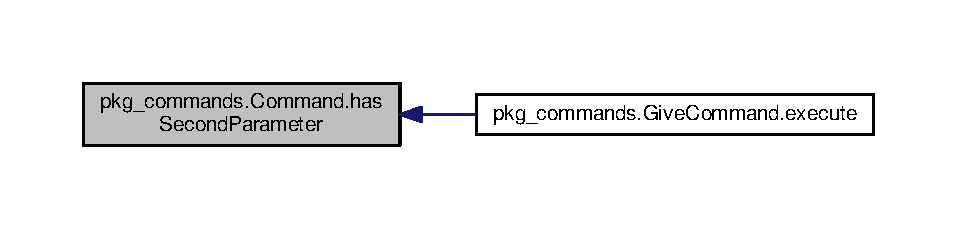
\includegraphics[width=350pt]{classpkg__commands_1_1Command_add688a76d80576c34f23927da19b9e2d_icgraph}
\end{center}
\end{figure}


\hypertarget{classpkg__commands_1_1Command_ae210ff216fe908b111ba1c988a963d13}{\index{pkg\-\_\-commands\-::\-Command@{pkg\-\_\-commands\-::\-Command}!set\-Message@{set\-Message}}
\index{set\-Message@{set\-Message}!pkg_commands::Command@{pkg\-\_\-commands\-::\-Command}}
\subsubsection[{set\-Message}]{\setlength{\rightskip}{0pt plus 5cm}void pkg\-\_\-commands.\-Command.\-set\-Message (
\begin{DoxyParamCaption}
\item[{String}]{message}
\end{DoxyParamCaption}
)\hspace{0.3cm}{\ttfamily [protected]}}}\label{classpkg__commands_1_1Command_ae210ff216fe908b111ba1c988a963d13}


Message field setter. 


\begin{DoxyParams}{Parameters}
{\em message} & The message to set \\
\hline
\end{DoxyParams}


Definition at line \hyperlink{Command_8java_source_l00089}{89} of file \hyperlink{Command_8java_source}{Command.\-java}.



Referenced by \hyperlink{BeamerCommand_8java_source_l00067}{pkg\-\_\-commands.\-Beamer\-Command.\-charge()}, \hyperlink{CreditsCommand_8java_source_l00023}{pkg\-\_\-commands.\-Credits\-Command.\-execute()}, \hyperlink{InventoryCommand_8java_source_l00023}{pkg\-\_\-commands.\-Inventory\-Command.\-execute()}, \hyperlink{LookCommand_8java_source_l00026}{pkg\-\_\-commands.\-Look\-Command.\-execute()}, \hyperlink{TakeCommand_8java_source_l00027}{pkg\-\_\-commands.\-Take\-Command.\-execute()}, \hyperlink{DropCommand_8java_source_l00027}{pkg\-\_\-commands.\-Drop\-Command.\-execute()}, \hyperlink{TalkCommand_8java_source_l00027}{pkg\-\_\-commands.\-Talk\-Command.\-execute()}, \hyperlink{EatCommand_8java_source_l00028}{pkg\-\_\-commands.\-Eat\-Command.\-execute()}, \hyperlink{ThrowCommand_8java_source_l00028}{pkg\-\_\-commands.\-Throw\-Command.\-execute()}, \hyperlink{GiveCommand_8java_source_l00029}{pkg\-\_\-commands.\-Give\-Command.\-execute()}, \hyperlink{TestCommand_8java_source_l00032}{pkg\-\_\-commands.\-Test\-Command.\-execute()}, \hyperlink{GoCommand_8java_source_l00032}{pkg\-\_\-commands.\-Go\-Command.\-execute()}, \hyperlink{HelpCommand_8java_source_l00033}{pkg\-\_\-commands.\-Help\-Command.\-execute()}, and \hyperlink{GoCommand_8java_source_l00071}{pkg\-\_\-commands.\-Go\-Command.\-go\-Room\-No\-Check()}.


\begin{DoxyCode}
00089                                               \{
00090         this.message = message;
00091     \}
\end{DoxyCode}


Here is the caller graph for this function\-:
\nopagebreak
\begin{figure}[H]
\begin{center}
\leavevmode
\includegraphics[width=350pt]{classpkg__commands_1_1Command_ae210ff216fe908b111ba1c988a963d13_icgraph}
\end{center}
\end{figure}


\hypertarget{classpkg__commands_1_1Command_a18446243a5fd360e9341b4b141c0cccc}{\index{pkg\-\_\-commands\-::\-Command@{pkg\-\_\-commands\-::\-Command}!set\-Parameter@{set\-Parameter}}
\index{set\-Parameter@{set\-Parameter}!pkg_commands::Command@{pkg\-\_\-commands\-::\-Command}}
\subsubsection[{set\-Parameter}]{\setlength{\rightskip}{0pt plus 5cm}void pkg\-\_\-commands.\-Command.\-set\-Parameter (
\begin{DoxyParamCaption}
\item[{String}]{parameter}
\end{DoxyParamCaption}
)}}\label{classpkg__commands_1_1Command_a18446243a5fd360e9341b4b141c0cccc}


Parameter field setter. 


\begin{DoxyParams}{Parameters}
{\em parameter} & The parameter to set \\
\hline
\end{DoxyParams}


Definition at line \hyperlink{Command_8java_source_l00057}{57} of file \hyperlink{Command_8java_source}{Command.\-java}.


\begin{DoxyCode}
00057                                                \{
00058         this.parameter = parameter;
00059     \}
\end{DoxyCode}
\hypertarget{classpkg__commands_1_1Command_af6de3828c27cd491ad24c4a97d69e856}{\index{pkg\-\_\-commands\-::\-Command@{pkg\-\_\-commands\-::\-Command}!set\-Second\-Parameter@{set\-Second\-Parameter}}
\index{set\-Second\-Parameter@{set\-Second\-Parameter}!pkg_commands::Command@{pkg\-\_\-commands\-::\-Command}}
\subsubsection[{set\-Second\-Parameter}]{\setlength{\rightskip}{0pt plus 5cm}void pkg\-\_\-commands.\-Command.\-set\-Second\-Parameter (
\begin{DoxyParamCaption}
\item[{String}]{parameter}
\end{DoxyParamCaption}
)}}\label{classpkg__commands_1_1Command_af6de3828c27cd491ad24c4a97d69e856}


Second Parameter field setter. 


\begin{DoxyParams}{Parameters}
{\em parameter} & The second parameter to set \\
\hline
\end{DoxyParams}


Definition at line \hyperlink{Command_8java_source_l00065}{65} of file \hyperlink{Command_8java_source}{Command.\-java}.


\begin{DoxyCode}
00065                                                      \{
00066         secondParameter = parameter;
00067     \}
\end{DoxyCode}


The documentation for this class was generated from the following file\-:\begin{DoxyCompactItemize}
\item 
pkg\-\_\-commands/\hyperlink{Command_8java}{Command.\-java}\end{DoxyCompactItemize}

\hypertarget{enumpkg__parsing_1_1CommandWord}{\section{pkg\-\_\-parsing.\-Command\-Word Enum Reference}
\label{enumpkg__parsing_1_1CommandWord}\index{pkg\-\_\-parsing.\-Command\-Word@{pkg\-\_\-parsing.\-Command\-Word}}
}


Representations for all the valid command words for the game.  




Collaboration diagram for pkg\-\_\-parsing.\-Command\-Word\-:
\nopagebreak
\begin{figure}[H]
\begin{center}
\leavevmode
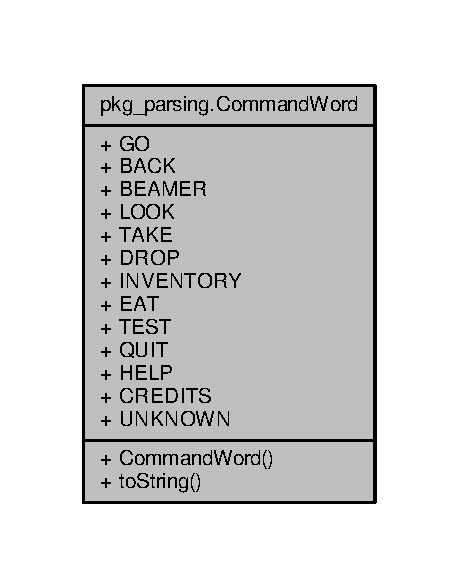
\includegraphics[width=220pt]{enumpkg__parsing_1_1CommandWord__coll__graph}
\end{center}
\end{figure}
\subsection*{Public Member Functions}
\begin{DoxyCompactItemize}
\item 
\hyperlink{enumpkg__parsing_1_1CommandWord_a7ff71159ae2c26835f5336580152d088}{Command\-Word} (String \hyperlink{enumpkg__parsing_1_1CommandWord_a2def2bcb3d7c2e973ad357341f4bd5b3}{command\-String})
\begin{DoxyCompactList}\small\item\em Initialise with the corresponding command word. \end{DoxyCompactList}\item 
String \hyperlink{enumpkg__parsing_1_1CommandWord_ab6d70b61b7418ce7dfa930bda64132c5}{to\-String} ()
\end{DoxyCompactItemize}
\subsection*{Public Attributes}
\begin{DoxyCompactItemize}
\item 
\hyperlink{enumpkg__parsing_1_1CommandWord_a82b58f470d1dbcf2a9e5826632d66524}{G\-O} =(\char`\"{}go\char`\"{})
\begin{DoxyCompactList}\small\item\em \char`\"{}go\char`\"{} command representation. \end{DoxyCompactList}\item 
\hyperlink{enumpkg__parsing_1_1CommandWord_a7c6d90e3ff897725acfab8f68b28a1b1}{B\-A\-C\-K} =(\char`\"{}back\char`\"{})
\begin{DoxyCompactList}\small\item\em \char`\"{}back\char`\"{} command representation. \end{DoxyCompactList}\item 
\hyperlink{enumpkg__parsing_1_1CommandWord_a4d1c3647eaf81664624ed5effc590be4}{B\-E\-A\-M\-E\-R} =(\char`\"{}beamer\char`\"{})
\begin{DoxyCompactList}\small\item\em \char`\"{}beamer\char`\"{} command representation. \end{DoxyCompactList}\item 
\hyperlink{enumpkg__parsing_1_1CommandWord_a56f571b76d6ef6d6c64f9b2081b53e86}{L\-O\-O\-K} =(\char`\"{}look\char`\"{})
\begin{DoxyCompactList}\small\item\em \char`\"{}look\char`\"{} command representation. \end{DoxyCompactList}\item 
\hyperlink{enumpkg__parsing_1_1CommandWord_ae5353500b91f141ae399403b5e87cc28}{T\-A\-K\-E} =(\char`\"{}take\char`\"{})
\begin{DoxyCompactList}\small\item\em \char`\"{}take\char`\"{} command representation. \end{DoxyCompactList}\item 
\hyperlink{enumpkg__parsing_1_1CommandWord_abc97c312acca6eef77cc303d91d2d811}{D\-R\-O\-P} =(\char`\"{}drop\char`\"{})
\begin{DoxyCompactList}\small\item\em \char`\"{}drop\char`\"{} command representation. \end{DoxyCompactList}\item 
\hyperlink{enumpkg__parsing_1_1CommandWord_a3dace936c35682fe74dad6714af270e4}{I\-N\-V\-E\-N\-T\-O\-R\-Y} =(\char`\"{}inventory\char`\"{})
\begin{DoxyCompactList}\small\item\em \char`\"{}inventory\char`\"{} command representation. \end{DoxyCompactList}\item 
\hyperlink{enumpkg__parsing_1_1CommandWord_a4fe488aea9cdd9ed9455682d42a300b3}{E\-A\-T} =(\char`\"{}eat\char`\"{})
\begin{DoxyCompactList}\small\item\em \char`\"{}eat\char`\"{} command representation. \end{DoxyCompactList}\item 
\hyperlink{enumpkg__parsing_1_1CommandWord_acf61cb32b4d651f87b2cd342761f9a79}{T\-E\-S\-T} =(\char`\"{}test\char`\"{})
\begin{DoxyCompactList}\small\item\em \char`\"{}test\char`\"{} command representation. \end{DoxyCompactList}\item 
\hyperlink{enumpkg__parsing_1_1CommandWord_a2f645cd1791d5576f42e1fe14d202c17}{Q\-U\-I\-T} =(\char`\"{}quit\char`\"{})
\begin{DoxyCompactList}\small\item\em \char`\"{}quit\char`\"{} command representation. \end{DoxyCompactList}\item 
\hyperlink{enumpkg__parsing_1_1CommandWord_ace035a3a624f4247b9f38c24eabe3f91}{H\-E\-L\-P} =(\char`\"{}help\char`\"{})
\begin{DoxyCompactList}\small\item\em \char`\"{}help\char`\"{} command representation. \end{DoxyCompactList}\item 
\hyperlink{enumpkg__parsing_1_1CommandWord_a4267a564de4d81cec28764b1eeb3ce22}{C\-R\-E\-D\-I\-T\-S} =(\char`\"{}credits\char`\"{})
\begin{DoxyCompactList}\small\item\em \char`\"{}credits\char`\"{} command representation. \end{DoxyCompactList}\item 
\hyperlink{enumpkg__parsing_1_1CommandWord_a7a089aad12d2934da530b785a3daab49}{U\-N\-K\-N\-O\-W\-N} =(\char`\"{}?\char`\"{})
\begin{DoxyCompactList}\small\item\em Unknown command representation. \end{DoxyCompactList}\end{DoxyCompactItemize}
\subsection*{Private Attributes}
\begin{DoxyCompactItemize}
\item 
String \hyperlink{enumpkg__parsing_1_1CommandWord_a2def2bcb3d7c2e973ad357341f4bd5b3}{command\-String}
\begin{DoxyCompactList}\small\item\em The String corresponding the the first word of the command. \end{DoxyCompactList}\end{DoxyCompactItemize}


\subsection{Detailed Description}
Representations for all the valid command words for the game. 

\begin{DoxyAuthor}{Author}
Rémi N\-I\-C\-O\-L\-E 
\end{DoxyAuthor}


Definition at line \hyperlink{CommandWord_8java_source_l00007}{7} of file \hyperlink{CommandWord_8java_source}{Command\-Word.\-java}.



\subsection{Constructor \& Destructor Documentation}
\hypertarget{enumpkg__parsing_1_1CommandWord_a7ff71159ae2c26835f5336580152d088}{\index{pkg\-\_\-parsing\-::\-Command\-Word@{pkg\-\_\-parsing\-::\-Command\-Word}!Command\-Word@{Command\-Word}}
\index{Command\-Word@{Command\-Word}!pkg_parsing::CommandWord@{pkg\-\_\-parsing\-::\-Command\-Word}}
\subsubsection[{Command\-Word}]{\setlength{\rightskip}{0pt plus 5cm}pkg\-\_\-parsing.\-Command\-Word.\-Command\-Word (
\begin{DoxyParamCaption}
\item[{String}]{command\-String}
\end{DoxyParamCaption}
)}}\label{enumpkg__parsing_1_1CommandWord_a7ff71159ae2c26835f5336580152d088}


Initialise with the corresponding command word. 


\begin{DoxyParams}{Parameters}
{\em command\-String} & The command string. \\
\hline
\end{DoxyParams}


Definition at line \hyperlink{CommandWord_8java_source_l00072}{72} of file \hyperlink{CommandWord_8java_source}{Command\-Word.\-java}.


\begin{DoxyCode}
00073     \{
00074         this.commandString = \hyperlink{enumpkg__parsing_1_1CommandWord_a2def2bcb3d7c2e973ad357341f4bd5b3}{commandString};
00075     \}
\end{DoxyCode}


\subsection{Member Function Documentation}
\hypertarget{enumpkg__parsing_1_1CommandWord_ab6d70b61b7418ce7dfa930bda64132c5}{\index{pkg\-\_\-parsing\-::\-Command\-Word@{pkg\-\_\-parsing\-::\-Command\-Word}!to\-String@{to\-String}}
\index{to\-String@{to\-String}!pkg_parsing::CommandWord@{pkg\-\_\-parsing\-::\-Command\-Word}}
\subsubsection[{to\-String}]{\setlength{\rightskip}{0pt plus 5cm}String pkg\-\_\-parsing.\-Command\-Word.\-to\-String (
\begin{DoxyParamCaption}
{}
\end{DoxyParamCaption}
)}}\label{enumpkg__parsing_1_1CommandWord_ab6d70b61b7418ce7dfa930bda64132c5}
\begin{DoxyReturn}{Returns}
The command word as a string. 
\end{DoxyReturn}


Definition at line \hyperlink{CommandWord_8java_source_l00080}{80} of file \hyperlink{CommandWord_8java_source}{Command\-Word.\-java}.


\begin{DoxyCode}
00081     \{
00082         \textcolor{keywordflow}{return} \hyperlink{enumpkg__parsing_1_1CommandWord_a2def2bcb3d7c2e973ad357341f4bd5b3}{commandString};
00083     \}
\end{DoxyCode}


\subsection{Member Data Documentation}
\hypertarget{enumpkg__parsing_1_1CommandWord_a7c6d90e3ff897725acfab8f68b28a1b1}{\index{pkg\-\_\-parsing\-::\-Command\-Word@{pkg\-\_\-parsing\-::\-Command\-Word}!B\-A\-C\-K@{B\-A\-C\-K}}
\index{B\-A\-C\-K@{B\-A\-C\-K}!pkg_parsing::CommandWord@{pkg\-\_\-parsing\-::\-Command\-Word}}
\subsubsection[{B\-A\-C\-K}]{\setlength{\rightskip}{0pt plus 5cm}pkg\-\_\-parsing.\-Command\-Word.\-B\-A\-C\-K =(\char`\"{}back\char`\"{})}}\label{enumpkg__parsing_1_1CommandWord_a7c6d90e3ff897725acfab8f68b28a1b1}


\char`\"{}back\char`\"{} command representation. 



Definition at line \hyperlink{CommandWord_8java_source_l00016}{16} of file \hyperlink{CommandWord_8java_source}{Command\-Word.\-java}.

\hypertarget{enumpkg__parsing_1_1CommandWord_a4d1c3647eaf81664624ed5effc590be4}{\index{pkg\-\_\-parsing\-::\-Command\-Word@{pkg\-\_\-parsing\-::\-Command\-Word}!B\-E\-A\-M\-E\-R@{B\-E\-A\-M\-E\-R}}
\index{B\-E\-A\-M\-E\-R@{B\-E\-A\-M\-E\-R}!pkg_parsing::CommandWord@{pkg\-\_\-parsing\-::\-Command\-Word}}
\subsubsection[{B\-E\-A\-M\-E\-R}]{\setlength{\rightskip}{0pt plus 5cm}pkg\-\_\-parsing.\-Command\-Word.\-B\-E\-A\-M\-E\-R =(\char`\"{}beamer\char`\"{})}}\label{enumpkg__parsing_1_1CommandWord_a4d1c3647eaf81664624ed5effc590be4}


\char`\"{}beamer\char`\"{} command representation. 



Definition at line \hyperlink{CommandWord_8java_source_l00020}{20} of file \hyperlink{CommandWord_8java_source}{Command\-Word.\-java}.

\hypertarget{enumpkg__parsing_1_1CommandWord_a2def2bcb3d7c2e973ad357341f4bd5b3}{\index{pkg\-\_\-parsing\-::\-Command\-Word@{pkg\-\_\-parsing\-::\-Command\-Word}!command\-String@{command\-String}}
\index{command\-String@{command\-String}!pkg_parsing::CommandWord@{pkg\-\_\-parsing\-::\-Command\-Word}}
\subsubsection[{command\-String}]{\setlength{\rightskip}{0pt plus 5cm}String pkg\-\_\-parsing.\-Command\-Word.\-command\-String\hspace{0.3cm}{\ttfamily [private]}}}\label{enumpkg__parsing_1_1CommandWord_a2def2bcb3d7c2e973ad357341f4bd5b3}


The String corresponding the the first word of the command. 



Definition at line \hyperlink{CommandWord_8java_source_l00065}{65} of file \hyperlink{CommandWord_8java_source}{Command\-Word.\-java}.

\hypertarget{enumpkg__parsing_1_1CommandWord_a4267a564de4d81cec28764b1eeb3ce22}{\index{pkg\-\_\-parsing\-::\-Command\-Word@{pkg\-\_\-parsing\-::\-Command\-Word}!C\-R\-E\-D\-I\-T\-S@{C\-R\-E\-D\-I\-T\-S}}
\index{C\-R\-E\-D\-I\-T\-S@{C\-R\-E\-D\-I\-T\-S}!pkg_parsing::CommandWord@{pkg\-\_\-parsing\-::\-Command\-Word}}
\subsubsection[{C\-R\-E\-D\-I\-T\-S}]{\setlength{\rightskip}{0pt plus 5cm}pkg\-\_\-parsing.\-Command\-Word.\-C\-R\-E\-D\-I\-T\-S =(\char`\"{}credits\char`\"{})}}\label{enumpkg__parsing_1_1CommandWord_a4267a564de4d81cec28764b1eeb3ce22}


\char`\"{}credits\char`\"{} command representation. 



Definition at line \hyperlink{CommandWord_8java_source_l00056}{56} of file \hyperlink{CommandWord_8java_source}{Command\-Word.\-java}.

\hypertarget{enumpkg__parsing_1_1CommandWord_abc97c312acca6eef77cc303d91d2d811}{\index{pkg\-\_\-parsing\-::\-Command\-Word@{pkg\-\_\-parsing\-::\-Command\-Word}!D\-R\-O\-P@{D\-R\-O\-P}}
\index{D\-R\-O\-P@{D\-R\-O\-P}!pkg_parsing::CommandWord@{pkg\-\_\-parsing\-::\-Command\-Word}}
\subsubsection[{D\-R\-O\-P}]{\setlength{\rightskip}{0pt plus 5cm}pkg\-\_\-parsing.\-Command\-Word.\-D\-R\-O\-P =(\char`\"{}drop\char`\"{})}}\label{enumpkg__parsing_1_1CommandWord_abc97c312acca6eef77cc303d91d2d811}


\char`\"{}drop\char`\"{} command representation. 



Definition at line \hyperlink{CommandWord_8java_source_l00032}{32} of file \hyperlink{CommandWord_8java_source}{Command\-Word.\-java}.

\hypertarget{enumpkg__parsing_1_1CommandWord_a4fe488aea9cdd9ed9455682d42a300b3}{\index{pkg\-\_\-parsing\-::\-Command\-Word@{pkg\-\_\-parsing\-::\-Command\-Word}!E\-A\-T@{E\-A\-T}}
\index{E\-A\-T@{E\-A\-T}!pkg_parsing::CommandWord@{pkg\-\_\-parsing\-::\-Command\-Word}}
\subsubsection[{E\-A\-T}]{\setlength{\rightskip}{0pt plus 5cm}pkg\-\_\-parsing.\-Command\-Word.\-E\-A\-T =(\char`\"{}eat\char`\"{})}}\label{enumpkg__parsing_1_1CommandWord_a4fe488aea9cdd9ed9455682d42a300b3}


\char`\"{}eat\char`\"{} command representation. 



Definition at line \hyperlink{CommandWord_8java_source_l00040}{40} of file \hyperlink{CommandWord_8java_source}{Command\-Word.\-java}.

\hypertarget{enumpkg__parsing_1_1CommandWord_a82b58f470d1dbcf2a9e5826632d66524}{\index{pkg\-\_\-parsing\-::\-Command\-Word@{pkg\-\_\-parsing\-::\-Command\-Word}!G\-O@{G\-O}}
\index{G\-O@{G\-O}!pkg_parsing::CommandWord@{pkg\-\_\-parsing\-::\-Command\-Word}}
\subsubsection[{G\-O}]{\setlength{\rightskip}{0pt plus 5cm}pkg\-\_\-parsing.\-Command\-Word.\-G\-O =(\char`\"{}go\char`\"{})}}\label{enumpkg__parsing_1_1CommandWord_a82b58f470d1dbcf2a9e5826632d66524}


\char`\"{}go\char`\"{} command representation. 



Definition at line \hyperlink{CommandWord_8java_source_l00012}{12} of file \hyperlink{CommandWord_8java_source}{Command\-Word.\-java}.

\hypertarget{enumpkg__parsing_1_1CommandWord_ace035a3a624f4247b9f38c24eabe3f91}{\index{pkg\-\_\-parsing\-::\-Command\-Word@{pkg\-\_\-parsing\-::\-Command\-Word}!H\-E\-L\-P@{H\-E\-L\-P}}
\index{H\-E\-L\-P@{H\-E\-L\-P}!pkg_parsing::CommandWord@{pkg\-\_\-parsing\-::\-Command\-Word}}
\subsubsection[{H\-E\-L\-P}]{\setlength{\rightskip}{0pt plus 5cm}pkg\-\_\-parsing.\-Command\-Word.\-H\-E\-L\-P =(\char`\"{}help\char`\"{})}}\label{enumpkg__parsing_1_1CommandWord_ace035a3a624f4247b9f38c24eabe3f91}


\char`\"{}help\char`\"{} command representation. 



Definition at line \hyperlink{CommandWord_8java_source_l00052}{52} of file \hyperlink{CommandWord_8java_source}{Command\-Word.\-java}.

\hypertarget{enumpkg__parsing_1_1CommandWord_a3dace936c35682fe74dad6714af270e4}{\index{pkg\-\_\-parsing\-::\-Command\-Word@{pkg\-\_\-parsing\-::\-Command\-Word}!I\-N\-V\-E\-N\-T\-O\-R\-Y@{I\-N\-V\-E\-N\-T\-O\-R\-Y}}
\index{I\-N\-V\-E\-N\-T\-O\-R\-Y@{I\-N\-V\-E\-N\-T\-O\-R\-Y}!pkg_parsing::CommandWord@{pkg\-\_\-parsing\-::\-Command\-Word}}
\subsubsection[{I\-N\-V\-E\-N\-T\-O\-R\-Y}]{\setlength{\rightskip}{0pt plus 5cm}pkg\-\_\-parsing.\-Command\-Word.\-I\-N\-V\-E\-N\-T\-O\-R\-Y =(\char`\"{}inventory\char`\"{})}}\label{enumpkg__parsing_1_1CommandWord_a3dace936c35682fe74dad6714af270e4}


\char`\"{}inventory\char`\"{} command representation. 



Definition at line \hyperlink{CommandWord_8java_source_l00036}{36} of file \hyperlink{CommandWord_8java_source}{Command\-Word.\-java}.

\hypertarget{enumpkg__parsing_1_1CommandWord_a56f571b76d6ef6d6c64f9b2081b53e86}{\index{pkg\-\_\-parsing\-::\-Command\-Word@{pkg\-\_\-parsing\-::\-Command\-Word}!L\-O\-O\-K@{L\-O\-O\-K}}
\index{L\-O\-O\-K@{L\-O\-O\-K}!pkg_parsing::CommandWord@{pkg\-\_\-parsing\-::\-Command\-Word}}
\subsubsection[{L\-O\-O\-K}]{\setlength{\rightskip}{0pt plus 5cm}pkg\-\_\-parsing.\-Command\-Word.\-L\-O\-O\-K =(\char`\"{}look\char`\"{})}}\label{enumpkg__parsing_1_1CommandWord_a56f571b76d6ef6d6c64f9b2081b53e86}


\char`\"{}look\char`\"{} command representation. 



Definition at line \hyperlink{CommandWord_8java_source_l00024}{24} of file \hyperlink{CommandWord_8java_source}{Command\-Word.\-java}.

\hypertarget{enumpkg__parsing_1_1CommandWord_a2f645cd1791d5576f42e1fe14d202c17}{\index{pkg\-\_\-parsing\-::\-Command\-Word@{pkg\-\_\-parsing\-::\-Command\-Word}!Q\-U\-I\-T@{Q\-U\-I\-T}}
\index{Q\-U\-I\-T@{Q\-U\-I\-T}!pkg_parsing::CommandWord@{pkg\-\_\-parsing\-::\-Command\-Word}}
\subsubsection[{Q\-U\-I\-T}]{\setlength{\rightskip}{0pt plus 5cm}pkg\-\_\-parsing.\-Command\-Word.\-Q\-U\-I\-T =(\char`\"{}quit\char`\"{})}}\label{enumpkg__parsing_1_1CommandWord_a2f645cd1791d5576f42e1fe14d202c17}


\char`\"{}quit\char`\"{} command representation. 



Definition at line \hyperlink{CommandWord_8java_source_l00048}{48} of file \hyperlink{CommandWord_8java_source}{Command\-Word.\-java}.

\hypertarget{enumpkg__parsing_1_1CommandWord_ae5353500b91f141ae399403b5e87cc28}{\index{pkg\-\_\-parsing\-::\-Command\-Word@{pkg\-\_\-parsing\-::\-Command\-Word}!T\-A\-K\-E@{T\-A\-K\-E}}
\index{T\-A\-K\-E@{T\-A\-K\-E}!pkg_parsing::CommandWord@{pkg\-\_\-parsing\-::\-Command\-Word}}
\subsubsection[{T\-A\-K\-E}]{\setlength{\rightskip}{0pt plus 5cm}pkg\-\_\-parsing.\-Command\-Word.\-T\-A\-K\-E =(\char`\"{}take\char`\"{})}}\label{enumpkg__parsing_1_1CommandWord_ae5353500b91f141ae399403b5e87cc28}


\char`\"{}take\char`\"{} command representation. 



Definition at line \hyperlink{CommandWord_8java_source_l00028}{28} of file \hyperlink{CommandWord_8java_source}{Command\-Word.\-java}.

\hypertarget{enumpkg__parsing_1_1CommandWord_acf61cb32b4d651f87b2cd342761f9a79}{\index{pkg\-\_\-parsing\-::\-Command\-Word@{pkg\-\_\-parsing\-::\-Command\-Word}!T\-E\-S\-T@{T\-E\-S\-T}}
\index{T\-E\-S\-T@{T\-E\-S\-T}!pkg_parsing::CommandWord@{pkg\-\_\-parsing\-::\-Command\-Word}}
\subsubsection[{T\-E\-S\-T}]{\setlength{\rightskip}{0pt plus 5cm}pkg\-\_\-parsing.\-Command\-Word.\-T\-E\-S\-T =(\char`\"{}test\char`\"{})}}\label{enumpkg__parsing_1_1CommandWord_acf61cb32b4d651f87b2cd342761f9a79}


\char`\"{}test\char`\"{} command representation. 



Definition at line \hyperlink{CommandWord_8java_source_l00044}{44} of file \hyperlink{CommandWord_8java_source}{Command\-Word.\-java}.

\hypertarget{enumpkg__parsing_1_1CommandWord_a7a089aad12d2934da530b785a3daab49}{\index{pkg\-\_\-parsing\-::\-Command\-Word@{pkg\-\_\-parsing\-::\-Command\-Word}!U\-N\-K\-N\-O\-W\-N@{U\-N\-K\-N\-O\-W\-N}}
\index{U\-N\-K\-N\-O\-W\-N@{U\-N\-K\-N\-O\-W\-N}!pkg_parsing::CommandWord@{pkg\-\_\-parsing\-::\-Command\-Word}}
\subsubsection[{U\-N\-K\-N\-O\-W\-N}]{\setlength{\rightskip}{0pt plus 5cm}pkg\-\_\-parsing.\-Command\-Word.\-U\-N\-K\-N\-O\-W\-N =(\char`\"{}?\char`\"{})}}\label{enumpkg__parsing_1_1CommandWord_a7a089aad12d2934da530b785a3daab49}


Unknown command representation. 



Definition at line \hyperlink{CommandWord_8java_source_l00060}{60} of file \hyperlink{CommandWord_8java_source}{Command\-Word.\-java}.



The documentation for this enum was generated from the following file\-:\begin{DoxyCompactItemize}
\item 
pkg\-\_\-parsing/\hyperlink{CommandWord_8java}{Command\-Word.\-java}\end{DoxyCompactItemize}

\hypertarget{classpkg__parsing_1_1CommandWords}{\section{pkg\-\_\-parsing.\-Command\-Words Class Reference}
\label{classpkg__parsing_1_1CommandWords}\index{pkg\-\_\-parsing.\-Command\-Words@{pkg\-\_\-parsing.\-Command\-Words}}
}


Collaboration diagram for pkg\-\_\-parsing.\-Command\-Words\-:
\nopagebreak
\begin{figure}[H]
\begin{center}
\leavevmode
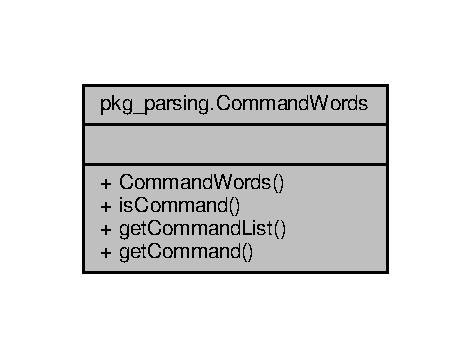
\includegraphics[width=226pt]{classpkg__parsing_1_1CommandWords__coll__graph}
\end{center}
\end{figure}
\subsection*{Public Member Functions}
\begin{DoxyCompactItemize}
\item 
\hyperlink{classpkg__parsing_1_1CommandWords_ac01e3b4727e741eb8add2eef27c8f7b7}{Command\-Words} ()
\item 
boolean \hyperlink{classpkg__parsing_1_1CommandWords_ab02b508bb42cbda758afe6cee5794216}{is\-Command} (String command)
\item 
String \hyperlink{classpkg__parsing_1_1CommandWords_a55f01013b1d051547ee3fa6605ea4c14}{get\-Command\-List} ()
\item 
\hyperlink{classpkg__commands_1_1Command}{Command} \hyperlink{classpkg__parsing_1_1CommandWords_a244829164976aa9444b3b1e84462ac5c}{get\-Command} (String command\-Word)
\end{DoxyCompactItemize}


\subsection{Detailed Description}
Class used to verify the commands given by the user. It contains all known commands and can verify if a String is a known command. \begin{DoxyAuthor}{Author}
Rémi N\-I\-C\-O\-L\-E 
\end{DoxyAuthor}


Definition at line \hyperlink{CommandWords_8java_source_l00017}{17} of file \hyperlink{CommandWords_8java_source}{Command\-Words.\-java}.



\subsection{Constructor \& Destructor Documentation}
\hypertarget{classpkg__parsing_1_1CommandWords_ac01e3b4727e741eb8add2eef27c8f7b7}{\index{pkg\-\_\-parsing\-::\-Command\-Words@{pkg\-\_\-parsing\-::\-Command\-Words}!Command\-Words@{Command\-Words}}
\index{Command\-Words@{Command\-Words}!pkg_parsing::CommandWords@{pkg\-\_\-parsing\-::\-Command\-Words}}
\subsubsection[{Command\-Words}]{\setlength{\rightskip}{0pt plus 5cm}pkg\-\_\-parsing.\-Command\-Words.\-Command\-Words (
\begin{DoxyParamCaption}
{}
\end{DoxyParamCaption}
)}}\label{classpkg__parsing_1_1CommandWords_ac01e3b4727e741eb8add2eef27c8f7b7}
\hyperlink{classpkg__parsing_1_1CommandWords}{Command\-Words} class constructor. 

Definition at line \hyperlink{CommandWords_8java_source_l00024}{24} of file \hyperlink{CommandWords_8java_source}{Command\-Words.\-java}.


\begin{DoxyCode}
00024                           \{
00025         commands = \textcolor{keyword}{new} HashMap<String, Command>();
00026         commands.put(\textcolor{stringliteral}{"go"}, \textcolor{keyword}{new} \hyperlink{classpkg__commands_1_1GoCommand}{GoCommand}());
00027         commands.put(\textcolor{stringliteral}{"back"}, \textcolor{keyword}{new} \hyperlink{classpkg__commands_1_1BackCommand}{BackCommand}());
00028         commands.put(\textcolor{stringliteral}{"beamer"}, \textcolor{keyword}{new} \hyperlink{classpkg__commands_1_1BeamerCommand}{BeamerCommand}());
00029         commands.put(\textcolor{stringliteral}{"look"}, \textcolor{keyword}{new} \hyperlink{classpkg__commands_1_1LookCommand}{LookCommand}());
00030         commands.put(\textcolor{stringliteral}{"take"}, \textcolor{keyword}{new} \hyperlink{classpkg__commands_1_1TakeCommand}{TakeCommand}());
00031         commands.put(\textcolor{stringliteral}{"drop"}, \textcolor{keyword}{new} \hyperlink{classpkg__commands_1_1DropCommand}{DropCommand}());
00032         commands.put(\textcolor{stringliteral}{"inventory"}, \textcolor{keyword}{new} \hyperlink{classpkg__commands_1_1InventoryCommand}{InventoryCommand}());
00033         commands.put(\textcolor{stringliteral}{"eat"}, \textcolor{keyword}{new} \hyperlink{classpkg__commands_1_1EatCommand}{EatCommand}());
00034         commands.put(\textcolor{stringliteral}{"test"}, \textcolor{keyword}{new} \hyperlink{classpkg__commands_1_1TestCommand}{TestCommand}());
00035         commands.put(\textcolor{stringliteral}{"talk"}, \textcolor{keyword}{new} \hyperlink{classpkg__commands_1_1TalkCommand}{TalkCommand}());
00036         commands.put(\textcolor{stringliteral}{"give"}, \textcolor{keyword}{new} \hyperlink{classpkg__commands_1_1GiveCommand}{GiveCommand}());
00037         commands.put(\textcolor{stringliteral}{"quit"}, \textcolor{keyword}{new} \hyperlink{classpkg__commands_1_1QuitCommand}{QuitCommand}());
00038         commands.put(\textcolor{stringliteral}{"help"}, \textcolor{keyword}{new} \hyperlink{classpkg__commands_1_1HelpCommand}{HelpCommand}());
00039         commands.put(\textcolor{stringliteral}{"credits"}, \textcolor{keyword}{new} \hyperlink{classpkg__commands_1_1CreditsCommand}{CreditsCommand}());
00040     \}
\end{DoxyCode}


\subsection{Member Function Documentation}
\hypertarget{classpkg__parsing_1_1CommandWords_a244829164976aa9444b3b1e84462ac5c}{\index{pkg\-\_\-parsing\-::\-Command\-Words@{pkg\-\_\-parsing\-::\-Command\-Words}!get\-Command@{get\-Command}}
\index{get\-Command@{get\-Command}!pkg_parsing::CommandWords@{pkg\-\_\-parsing\-::\-Command\-Words}}
\subsubsection[{get\-Command}]{\setlength{\rightskip}{0pt plus 5cm}{\bf Command} pkg\-\_\-parsing.\-Command\-Words.\-get\-Command (
\begin{DoxyParamCaption}
\item[{String}]{command\-Word}
\end{DoxyParamCaption}
)}}\label{classpkg__parsing_1_1CommandWords_a244829164976aa9444b3b1e84462ac5c}
Find the \hyperlink{enumpkg__parsing_1_1CommandWord}{Command\-Word} associated with a command word. 
\begin{DoxyParams}{Parameters}
{\em command\-Word} & The word to look up. \\
\hline
\end{DoxyParams}
\begin{DoxyReturn}{Returns}
The Command correspondng to command\-Word, or null if it is not a valid command word. 
\end{DoxyReturn}


Definition at line \hyperlink{CommandWords_8java_source_l00070}{70} of file \hyperlink{CommandWords_8java_source}{Command\-Words.\-java}.


\begin{DoxyCode}
00071     \{
00072         \textcolor{keywordflow}{return} commands.get(commandWord);
00073     \}
\end{DoxyCode}
\hypertarget{classpkg__parsing_1_1CommandWords_a55f01013b1d051547ee3fa6605ea4c14}{\index{pkg\-\_\-parsing\-::\-Command\-Words@{pkg\-\_\-parsing\-::\-Command\-Words}!get\-Command\-List@{get\-Command\-List}}
\index{get\-Command\-List@{get\-Command\-List}!pkg_parsing::CommandWords@{pkg\-\_\-parsing\-::\-Command\-Words}}
\subsubsection[{get\-Command\-List}]{\setlength{\rightskip}{0pt plus 5cm}String pkg\-\_\-parsing.\-Command\-Words.\-get\-Command\-List (
\begin{DoxyParamCaption}
{}
\end{DoxyParamCaption}
)}}\label{classpkg__parsing_1_1CommandWords_a55f01013b1d051547ee3fa6605ea4c14}
Getter for the known\-Commands field. \begin{DoxyReturn}{Returns}
The list of available commands 
\end{DoxyReturn}


Definition at line \hyperlink{CommandWords_8java_source_l00055}{55} of file \hyperlink{CommandWords_8java_source}{Command\-Words.\-java}.


\begin{DoxyCode}
00055                                    \{
00056         String commandsString = \textcolor{stringliteral}{""};
00057         Iterator<String> it = commands.keySet().iterator();
00058         \textcolor{keywordflow}{while}(it.hasNext()) \{
00059             String command = it.next();
00060             commandsString += command + ((it.hasNext())? \textcolor{stringliteral}{", "} : \textcolor{stringliteral}{"."});
00061         \}
00062         \textcolor{keywordflow}{return} commandsString;
00063     \}
\end{DoxyCode}
\hypertarget{classpkg__parsing_1_1CommandWords_ab02b508bb42cbda758afe6cee5794216}{\index{pkg\-\_\-parsing\-::\-Command\-Words@{pkg\-\_\-parsing\-::\-Command\-Words}!is\-Command@{is\-Command}}
\index{is\-Command@{is\-Command}!pkg_parsing::CommandWords@{pkg\-\_\-parsing\-::\-Command\-Words}}
\subsubsection[{is\-Command}]{\setlength{\rightskip}{0pt plus 5cm}boolean pkg\-\_\-parsing.\-Command\-Words.\-is\-Command (
\begin{DoxyParamCaption}
\item[{String}]{command}
\end{DoxyParamCaption}
)}}\label{classpkg__parsing_1_1CommandWords_ab02b508bb42cbda758afe6cee5794216}
Check if the command is known. 
\begin{DoxyParams}{Parameters}
{\em command} & The command to check \\
\hline
\end{DoxyParams}
\begin{DoxyReturn}{Returns}
True if and only if the command is known. 
\end{DoxyReturn}


Definition at line \hyperlink{CommandWords_8java_source_l00047}{47} of file \hyperlink{CommandWords_8java_source}{Command\-Words.\-java}.


\begin{DoxyCode}
00047                                              \{
00048         \textcolor{keywordflow}{return} commands.containsKey(command);
00049     \}
\end{DoxyCode}


The documentation for this class was generated from the following file\-:\begin{DoxyCompactItemize}
\item 
pkg\-\_\-parsing/\hyperlink{CommandWords_8java}{Command\-Words.\-java}\end{DoxyCompactItemize}

\hypertarget{classpkg__commands_1_1CreditsCommand}{\section{pkg\-\_\-commands.\-Credits\-Command Class Reference}
\label{classpkg__commands_1_1CreditsCommand}\index{pkg\-\_\-commands.\-Credits\-Command@{pkg\-\_\-commands.\-Credits\-Command}}
}


Inheritance diagram for pkg\-\_\-commands.\-Credits\-Command\-:
\nopagebreak
\begin{figure}[H]
\begin{center}
\leavevmode
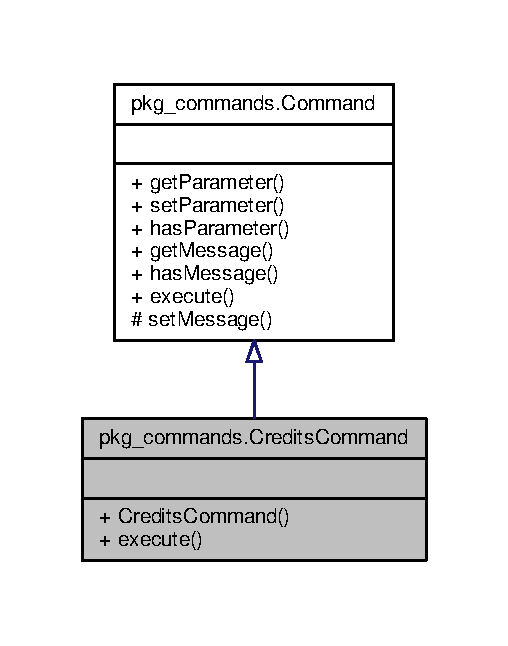
\includegraphics[width=244pt]{classpkg__commands_1_1CreditsCommand__inherit__graph}
\end{center}
\end{figure}


Collaboration diagram for pkg\-\_\-commands.\-Credits\-Command\-:
\nopagebreak
\begin{figure}[H]
\begin{center}
\leavevmode
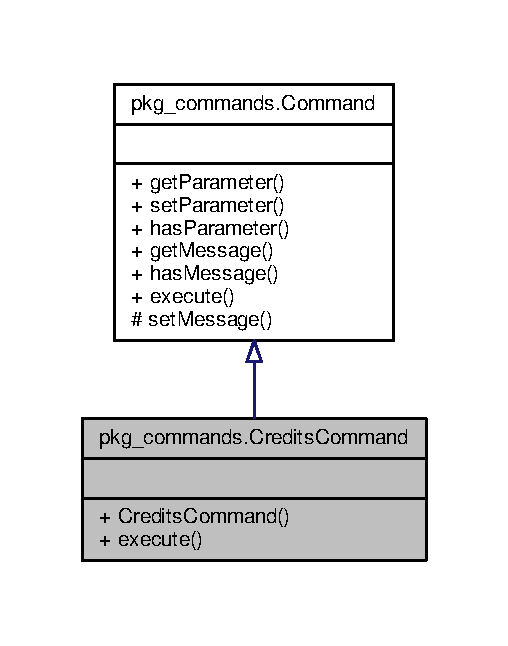
\includegraphics[width=244pt]{classpkg__commands_1_1CreditsCommand__coll__graph}
\end{center}
\end{figure}
\subsection*{Public Member Functions}
\begin{DoxyCompactItemize}
\item 
\hyperlink{classpkg__commands_1_1CreditsCommand_aa4338bdebb23612f95fa151ecd6f3bd2}{Credits\-Command} ()
\item 
boolean \hyperlink{classpkg__commands_1_1CreditsCommand_aad2b955c6c8a4c3536e6b937165b7790}{execute} (\hyperlink{classpkg__world_1_1Player}{Player} player)
\end{DoxyCompactItemize}
\subsection*{Additional Inherited Members}


\subsection{Detailed Description}
class \hyperlink{classpkg__commands_1_1CreditsCommand}{Credits\-Command} used to print the credits of the game \begin{DoxyAuthor}{Author}
Rémi Nicole 
\end{DoxyAuthor}


Definition at line \hyperlink{CreditsCommand_8java_source_l00009}{9} of file \hyperlink{CreditsCommand_8java_source}{Credits\-Command.\-java}.



\subsection{Constructor \& Destructor Documentation}
\hypertarget{classpkg__commands_1_1CreditsCommand_aa4338bdebb23612f95fa151ecd6f3bd2}{\index{pkg\-\_\-commands\-::\-Credits\-Command@{pkg\-\_\-commands\-::\-Credits\-Command}!Credits\-Command@{Credits\-Command}}
\index{Credits\-Command@{Credits\-Command}!pkg_commands::CreditsCommand@{pkg\-\_\-commands\-::\-Credits\-Command}}
\subsubsection[{Credits\-Command}]{\setlength{\rightskip}{0pt plus 5cm}pkg\-\_\-commands.\-Credits\-Command.\-Credits\-Command (
\begin{DoxyParamCaption}
{}
\end{DoxyParamCaption}
)}}\label{classpkg__commands_1_1CreditsCommand_aa4338bdebb23612f95fa151ecd6f3bd2}
Constructor for \hyperlink{classpkg__commands_1_1CreditsCommand}{Credits\-Command} 

Definition at line \hyperlink{CreditsCommand_8java_source_l00014}{14} of file \hyperlink{CreditsCommand_8java_source}{Credits\-Command.\-java}.


\begin{DoxyCode}
00014                            \{
00015 
00016     \}
\end{DoxyCode}


\subsection{Member Function Documentation}
\hypertarget{classpkg__commands_1_1CreditsCommand_aad2b955c6c8a4c3536e6b937165b7790}{\index{pkg\-\_\-commands\-::\-Credits\-Command@{pkg\-\_\-commands\-::\-Credits\-Command}!execute@{execute}}
\index{execute@{execute}!pkg_commands::CreditsCommand@{pkg\-\_\-commands\-::\-Credits\-Command}}
\subsubsection[{execute}]{\setlength{\rightskip}{0pt plus 5cm}boolean pkg\-\_\-commands.\-Credits\-Command.\-execute (
\begin{DoxyParamCaption}
\item[{{\bf Player}}]{player}
\end{DoxyParamCaption}
)}}\label{classpkg__commands_1_1CreditsCommand_aad2b955c6c8a4c3536e6b937165b7790}
Save the credits into the message field. 
\begin{DoxyParams}{Parameters}
{\em player} & The player that called this command \\
\hline
\end{DoxyParams}
\begin{DoxyReturn}{Returns}
False because it is not the quit command 
\end{DoxyReturn}


Definition at line \hyperlink{CreditsCommand_8java_source_l00023}{23} of file \hyperlink{CreditsCommand_8java_source}{Credits\-Command.\-java}.



References \hyperlink{Command_8java_source_l00058}{pkg\-\_\-commands.\-Command.\-set\-Message()}.


\begin{DoxyCode}
00023                                           \{
00024         \hyperlink{classpkg__commands_1_1Command_ae210ff216fe908b111ba1c988a963d13}{setMessage}(\textcolor{stringliteral}{"Temperate rainforest photo (cc-by-nc-nd) : myheimu
       (http://www.fotopedia.com/wiki/Temperate\_rainforest#!/items/flickr-7995237868)\(\backslash\)n"}
00025                 + \textcolor{stringliteral}{"Taiga photo (public domain) : Becker0804
       (https://commons.wikimedia.org/wiki/File:Talkessel\_von\_Werchojansk.JPG)\(\backslash\)n"}
00026                 + \textcolor{stringliteral}{"Alpine tundra photo (public domain) : Zewu
       (https://en.wikipedia.org/wiki/File:Tarfala\_Valley\_-\_Sweden.jpg)\(\backslash\)n"}
00027                 + \textcolor{stringliteral}{"Steppe photo (cc-by-sa) : Matt Lavin
       (http://www.fotopedia.com/wiki/Steppe#!/items/flickr-7495949260)\(\backslash\)n"}
00028                 + \textcolor{stringliteral}{"Lava tube photo : Tim Laman
       (http://science.nationalgeographic.com/science/photos/caves-gallery/#/lava-tube-cave\_1036\_600x450.jpg)\(\backslash\)n"}
00029                 + \textcolor{stringliteral}{"Polar desert photo (cc-by) : Stephen Hudson
       (https://commons.wikimedia.org/wiki/File:AntarcticaDomeCSnow.jpg)\(\backslash\)n"}
00030                 + \textcolor{stringliteral}{"Thar desert photo (cc-by-sa) : Gégard JANOT
       (https://commons.wikimedia.org/wiki/File:D%C3%A9sert\_du\_Rajasthan.jpg)\(\backslash\)n"}
00031                 + \textcolor{stringliteral}{"Savanna photo (public domain) : United States Geological Survey
       (https://commons.wikimedia.org/wiki/File:Oldoinyolengai.jpg)"});
00032         \textcolor{keywordflow}{return} \textcolor{keyword}{false};
00033     \}
\end{DoxyCode}


Here is the call graph for this function\-:
\nopagebreak
\begin{figure}[H]
\begin{center}
\leavevmode
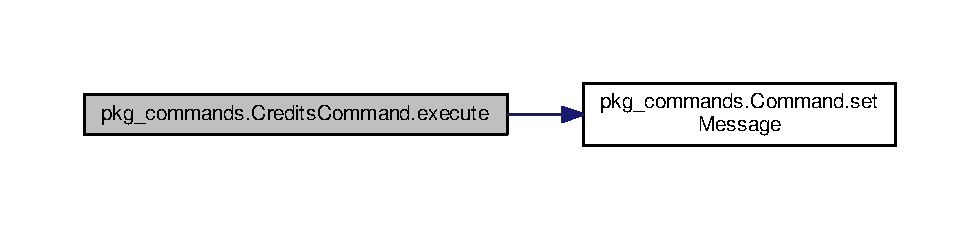
\includegraphics[width=350pt]{classpkg__commands_1_1CreditsCommand_aad2b955c6c8a4c3536e6b937165b7790_cgraph}
\end{center}
\end{figure}




The documentation for this class was generated from the following file\-:\begin{DoxyCompactItemize}
\item 
pkg\-\_\-commands/\hyperlink{CreditsCommand_8java}{Credits\-Command.\-java}\end{DoxyCompactItemize}

\hypertarget{classpkg__commands_1_1DropCommand}{\section{pkg\-\_\-commands.\-Drop\-Command Class Reference}
\label{classpkg__commands_1_1DropCommand}\index{pkg\-\_\-commands.\-Drop\-Command@{pkg\-\_\-commands.\-Drop\-Command}}
}


Inheritance diagram for pkg\-\_\-commands.\-Drop\-Command\-:
\nopagebreak
\begin{figure}[H]
\begin{center}
\leavevmode
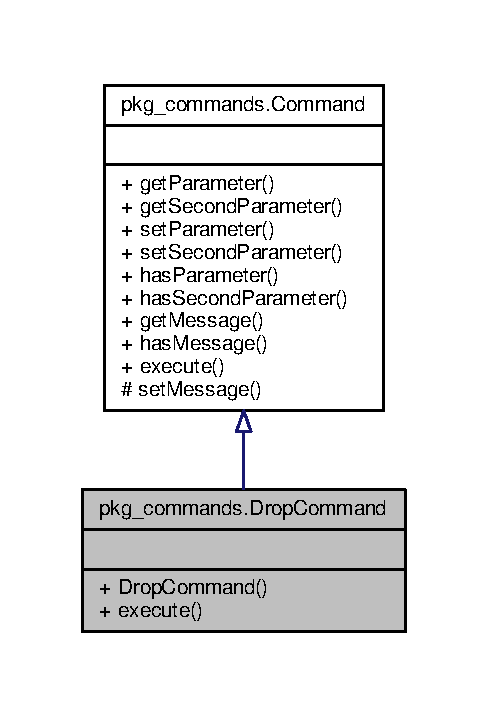
\includegraphics[width=234pt]{classpkg__commands_1_1DropCommand__inherit__graph}
\end{center}
\end{figure}


Collaboration diagram for pkg\-\_\-commands.\-Drop\-Command\-:
\nopagebreak
\begin{figure}[H]
\begin{center}
\leavevmode
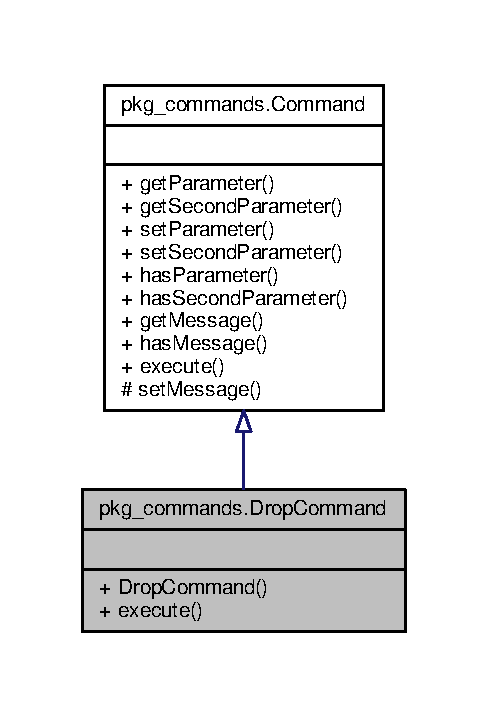
\includegraphics[width=234pt]{classpkg__commands_1_1DropCommand__coll__graph}
\end{center}
\end{figure}
\subsection*{Public Member Functions}
\begin{DoxyCompactItemize}
\item 
\hyperlink{classpkg__commands_1_1DropCommand_a2e755d7f4b0735183553d5d97d624f0c}{Drop\-Command} ()
\item 
boolean \hyperlink{classpkg__commands_1_1DropCommand_a742e37b2d2dd4e111130811ee2f4dd0b}{execute} (\hyperlink{classpkg__world_1_1Player}{Player} player)  throws No\-Argument\-Exception,\-Illegal\-Argument\-Exception 
\end{DoxyCompactItemize}
\subsection*{Additional Inherited Members}


\subsection{Detailed Description}
class \hyperlink{classpkg__commands_1_1DropCommand}{Drop\-Command} used to make the player drop an Item \begin{DoxyAuthor}{Author}
Rémi Nicole 
\end{DoxyAuthor}


Definition at line \hyperlink{DropCommand_8java_source_l00011}{11} of file \hyperlink{DropCommand_8java_source}{Drop\-Command.\-java}.



\subsection{Constructor \& Destructor Documentation}
\hypertarget{classpkg__commands_1_1DropCommand_a2e755d7f4b0735183553d5d97d624f0c}{\index{pkg\-\_\-commands\-::\-Drop\-Command@{pkg\-\_\-commands\-::\-Drop\-Command}!Drop\-Command@{Drop\-Command}}
\index{Drop\-Command@{Drop\-Command}!pkg_commands::DropCommand@{pkg\-\_\-commands\-::\-Drop\-Command}}
\subsubsection[{Drop\-Command}]{\setlength{\rightskip}{0pt plus 5cm}pkg\-\_\-commands.\-Drop\-Command.\-Drop\-Command (
\begin{DoxyParamCaption}
{}
\end{DoxyParamCaption}
)}}\label{classpkg__commands_1_1DropCommand_a2e755d7f4b0735183553d5d97d624f0c}
Constructor for \hyperlink{classpkg__commands_1_1DropCommand}{Drop\-Command} 

Definition at line \hyperlink{DropCommand_8java_source_l00016}{16} of file \hyperlink{DropCommand_8java_source}{Drop\-Command.\-java}.


\begin{DoxyCode}
00016                         \{
00017 
00018     \}
\end{DoxyCode}


\subsection{Member Function Documentation}
\hypertarget{classpkg__commands_1_1DropCommand_a742e37b2d2dd4e111130811ee2f4dd0b}{\index{pkg\-\_\-commands\-::\-Drop\-Command@{pkg\-\_\-commands\-::\-Drop\-Command}!execute@{execute}}
\index{execute@{execute}!pkg_commands::DropCommand@{pkg\-\_\-commands\-::\-Drop\-Command}}
\subsubsection[{execute}]{\setlength{\rightskip}{0pt plus 5cm}boolean pkg\-\_\-commands.\-Drop\-Command.\-execute (
\begin{DoxyParamCaption}
\item[{{\bf Player}}]{player}
\end{DoxyParamCaption}
) throws {\bf No\-Argument\-Exception},{\bf Illegal\-Argument\-Exception}}}\label{classpkg__commands_1_1DropCommand_a742e37b2d2dd4e111130811ee2f4dd0b}
Drop the Item through it's name in the parameter field. 
\begin{DoxyParams}{Parameters}
{\em player} & The player that called this command \\
\hline
\end{DoxyParams}

\begin{DoxyExceptions}{Exceptions}
{\em No\-Argument\-Exception} & When the user typed the command without parameter \\
\hline
{\em Illegal\-Argument\-Exception} & When the user typed a name other than any of the items in the Player's inventory \\
\hline
\end{DoxyExceptions}
\begin{DoxyReturn}{Returns}
False because it is not the quit command 
\end{DoxyReturn}


Definition at line \hyperlink{DropCommand_8java_source_l00027}{27} of file \hyperlink{DropCommand_8java_source}{Drop\-Command.\-java}.



References \hyperlink{Command_8java_source_l00034}{pkg\-\_\-commands.\-Command.\-get\-Parameter()}, \hyperlink{Command_8java_source_l00050}{pkg\-\_\-commands.\-Command.\-has\-Parameter()}, and \hyperlink{Command_8java_source_l00058}{pkg\-\_\-commands.\-Command.\-set\-Message()}.


\begin{DoxyCode}
00027                                                                                               \{
00028         \textcolor{keywordflow}{if}(\hyperlink{classpkg__commands_1_1Command_a02af95ab3f1898a66259ab7c177b6998}{hasParameter}()) \{
00029             \textcolor{keywordflow}{if}(player.hasItem(\hyperlink{classpkg__commands_1_1Command_a41c92d445be73ea9d62320c65efb8434}{getParameter}()))\{
00030                 player.dropObject(\hyperlink{classpkg__commands_1_1Command_a41c92d445be73ea9d62320c65efb8434}{getParameter}());
00031                 \hyperlink{classpkg__commands_1_1Command_ae210ff216fe908b111ba1c988a963d13}{setMessage}(\textcolor{stringliteral}{"Oh, dear. He took a"} + (((\textcolor{keyword}{new} String(\textcolor{stringliteral}{"aeiouy"})).contains(
      \hyperlink{classpkg__commands_1_1Command_a41c92d445be73ea9d62320c65efb8434}{getParameter}().substring(0,1)))? \textcolor{stringliteral}{"n "} : \textcolor{stringliteral}{" "}) + \hyperlink{classpkg__commands_1_1Command_a41c92d445be73ea9d62320c65efb8434}{getParameter}() + \textcolor{stringliteral}{"."});
00032             \} \textcolor{keywordflow}{else}
00033                 \textcolor{keywordflow}{throw} \textcolor{keyword}{new} IllegalArgumentException(\textcolor{stringliteral}{"If you want to drop that, you may have a mental
       disorder. As expected."});
00034         \} \textcolor{keywordflow}{else}
00035             \textcolor{keywordflow}{throw} \textcolor{keyword}{new} NoArgumentException(\textcolor{stringliteral}{"I agree. We both want you to drop dead."});
00036         \textcolor{keywordflow}{return} \textcolor{keyword}{false};
00037     \}
\end{DoxyCode}


Here is the call graph for this function\-:
\nopagebreak
\begin{figure}[H]
\begin{center}
\leavevmode
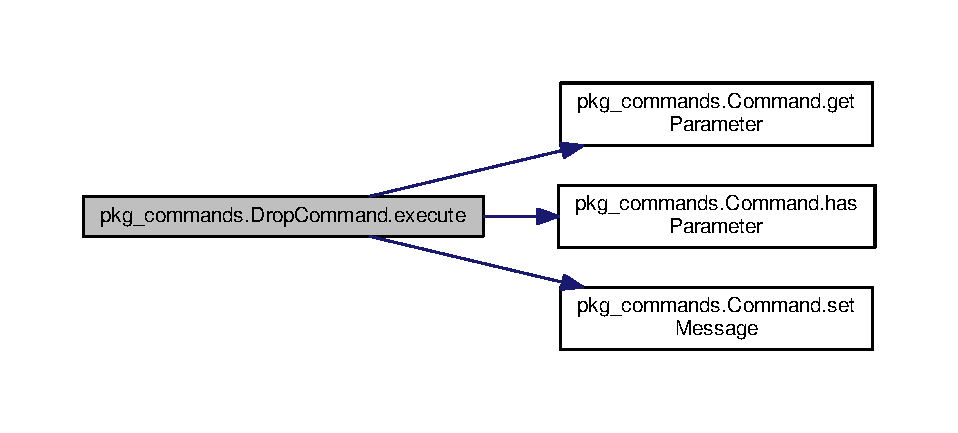
\includegraphics[width=350pt]{classpkg__commands_1_1DropCommand_a742e37b2d2dd4e111130811ee2f4dd0b_cgraph}
\end{center}
\end{figure}




The documentation for this class was generated from the following file\-:\begin{DoxyCompactItemize}
\item 
pkg\-\_\-commands/\hyperlink{DropCommand_8java}{Drop\-Command.\-java}\end{DoxyCompactItemize}

\hypertarget{classpkg__commands_1_1EatCommand}{\section{pkg\-\_\-commands.\-Eat\-Command Class Reference}
\label{classpkg__commands_1_1EatCommand}\index{pkg\-\_\-commands.\-Eat\-Command@{pkg\-\_\-commands.\-Eat\-Command}}
}


class \hyperlink{classpkg__commands_1_1EatCommand}{Eat\-Command} used to make the player eat an object.  




Inheritance diagram for pkg\-\_\-commands.\-Eat\-Command\-:\nopagebreak
\begin{figure}[H]
\begin{center}
\leavevmode
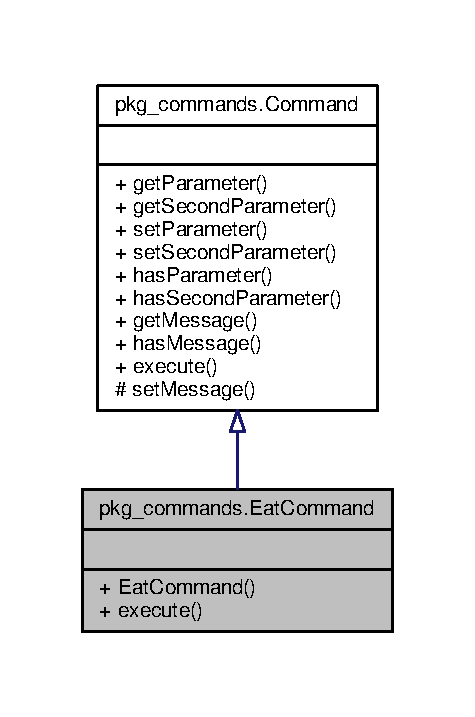
\includegraphics[width=228pt]{classpkg__commands_1_1EatCommand__inherit__graph}
\end{center}
\end{figure}


Collaboration diagram for pkg\-\_\-commands.\-Eat\-Command\-:\nopagebreak
\begin{figure}[H]
\begin{center}
\leavevmode
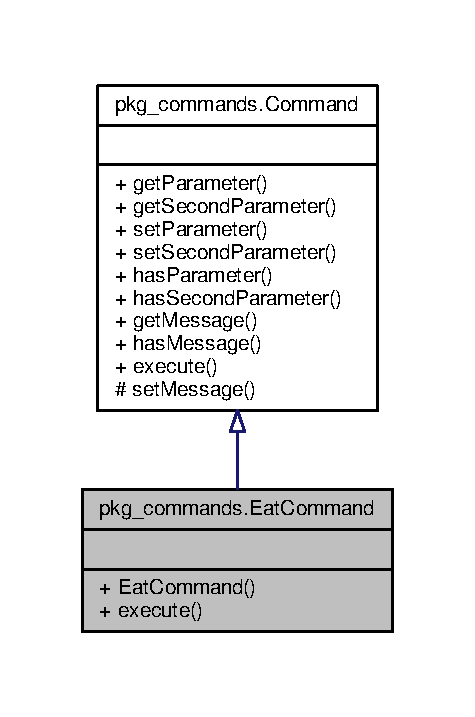
\includegraphics[width=228pt]{classpkg__commands_1_1EatCommand__coll__graph}
\end{center}
\end{figure}
\subsection*{Public Member Functions}
\begin{DoxyCompactItemize}
\item 
\hyperlink{classpkg__commands_1_1EatCommand_ad83dfae54a7d24140beff2b00201e065}{Eat\-Command} ()
\begin{DoxyCompactList}\small\item\em Constructor for \hyperlink{classpkg__commands_1_1EatCommand}{Eat\-Command}. \end{DoxyCompactList}\item 
boolean \hyperlink{classpkg__commands_1_1EatCommand_a2a600f09891aa076b3f630293de965f4}{execute} (\hyperlink{classpkg__world_1_1Player}{Player} player)  throws No\-Argument\-Exception,pkg\-\_\-exceptions.\-Illegal\-Argument\-Exception,\-Unauthorized\-Exception 
\begin{DoxyCompactList}\small\item\em Make the player eat an object. \end{DoxyCompactList}\end{DoxyCompactItemize}
\subsection*{Additional Inherited Members}


\subsection{Detailed Description}
class \hyperlink{classpkg__commands_1_1EatCommand}{Eat\-Command} used to make the player eat an object. 

\begin{DoxyAuthor}{Author}
Rémi Nicole 
\end{DoxyAuthor}


Definition at line \hyperlink{EatCommand_8java_source_l00010}{10} of file \hyperlink{EatCommand_8java_source}{Eat\-Command.\-java}.



\subsection{Constructor \& Destructor Documentation}
\hypertarget{classpkg__commands_1_1EatCommand_ad83dfae54a7d24140beff2b00201e065}{\index{pkg\-\_\-commands\-::\-Eat\-Command@{pkg\-\_\-commands\-::\-Eat\-Command}!Eat\-Command@{Eat\-Command}}
\index{Eat\-Command@{Eat\-Command}!pkg_commands::EatCommand@{pkg\-\_\-commands\-::\-Eat\-Command}}
\subsubsection[{Eat\-Command}]{\setlength{\rightskip}{0pt plus 5cm}pkg\-\_\-commands.\-Eat\-Command.\-Eat\-Command (
\begin{DoxyParamCaption}
{}
\end{DoxyParamCaption}
)}}\label{classpkg__commands_1_1EatCommand_ad83dfae54a7d24140beff2b00201e065}


Constructor for \hyperlink{classpkg__commands_1_1EatCommand}{Eat\-Command}. 



Definition at line \hyperlink{EatCommand_8java_source_l00015}{15} of file \hyperlink{EatCommand_8java_source}{Eat\-Command.\-java}.


\begin{DoxyCode}
00015                        \{
00016 
00017     \}
\end{DoxyCode}


\subsection{Member Function Documentation}
\hypertarget{classpkg__commands_1_1EatCommand_a2a600f09891aa076b3f630293de965f4}{\index{pkg\-\_\-commands\-::\-Eat\-Command@{pkg\-\_\-commands\-::\-Eat\-Command}!execute@{execute}}
\index{execute@{execute}!pkg_commands::EatCommand@{pkg\-\_\-commands\-::\-Eat\-Command}}
\subsubsection[{execute}]{\setlength{\rightskip}{0pt plus 5cm}boolean pkg\-\_\-commands.\-Eat\-Command.\-execute (
\begin{DoxyParamCaption}
\item[{{\bf Player}}]{player}
\end{DoxyParamCaption}
) throws {\bf No\-Argument\-Exception},{\bf pkg\-\_\-exceptions.\-Illegal\-Argument\-Exception},{\bf Unauthorized\-Exception}}}\label{classpkg__commands_1_1EatCommand_a2a600f09891aa076b3f630293de965f4}


Make the player eat an object. 

Only the \char`\"{}magiccookie\char`\"{} Item is eatable 
\begin{DoxyParams}{Parameters}
{\em player} & The player that called this command \\
\hline
\end{DoxyParams}

\begin{DoxyExceptions}{Exceptions}
{\em No\-Argument\-Exception} & When the user typed the command without parameter \\
\hline
{\em Illegal\-Argument\-Exception} & When the user typed a name other than any of the items in the Player's inventory \\
\hline
{\em Unauthorized\-Exception} & When the user tries to eat a non-\/eatable object \\
\hline
\end{DoxyExceptions}
\begin{DoxyReturn}{Returns}
False because it is not the quit command 
\end{DoxyReturn}


Definition at line \hyperlink{EatCommand_8java_source_l00028}{28} of file \hyperlink{EatCommand_8java_source}{Eat\-Command.\-java}.



References \hyperlink{Command_8java_source_l00034}{pkg\-\_\-commands.\-Command.\-get\-Parameter()}, \hyperlink{Command_8java_source_l00050}{pkg\-\_\-commands.\-Command.\-has\-Parameter()}, and \hyperlink{Command_8java_source_l00058}{pkg\-\_\-commands.\-Command.\-set\-Message()}.


\begin{DoxyCode}
00028                                                                                                            
                              \{
00029         \textcolor{keywordflow}{if}(\hyperlink{classpkg__commands_1_1Command_a02af95ab3f1898a66259ab7c177b6998}{hasParameter}()) \{
00030             \textcolor{keywordflow}{if}(player.hasItem(\hyperlink{classpkg__commands_1_1Command_a41c92d445be73ea9d62320c65efb8434}{getParameter}()))\{
00031                 \textcolor{keywordflow}{if}(\hyperlink{classpkg__commands_1_1Command_a41c92d445be73ea9d62320c65efb8434}{getParameter}().equals(\textcolor{stringliteral}{"magiccookie"})) \{
00032                     player.eatObject(\hyperlink{classpkg__commands_1_1Command_a41c92d445be73ea9d62320c65efb8434}{getParameter}());
00033                     player.setMaxWeight(player.getMaxWeight() + 100);
00034                     \hyperlink{classpkg__commands_1_1Command_ae210ff216fe908b111ba1c988a963d13}{setMessage}(\textcolor{stringliteral}{"You found an out of date \(\backslash\)"magic\(\backslash\)" cookie inside a cave and you
       just ate it.\(\backslash\)nNow you can carry more items. That's logic!"});
00035                 \} \textcolor{keywordflow}{else}
00036                     \textcolor{keywordflow}{throw} \textcolor{keyword}{new} \hyperlink{classpkg__exceptions_1_1UnauthorizedException}{UnauthorizedException}(\textcolor{stringliteral}{"If that's what you eat, I don't
       want to be invited to any of your meals.\(\backslash\)nI'm afraid I can't allow you to do that."});
00037             \} \textcolor{keywordflow}{else} 
00038                 \textcolor{keywordflow}{throw} \textcolor{keyword}{new} \hyperlink{classpkg__exceptions_1_1IllegalArgumentException}{pkg\_exceptions.IllegalArgumentException}(\textcolor{stringliteral}{"
      You don't have that. And I'm sure that if you did, it wouldn't be smart to eat that."});
00039         \} \textcolor{keywordflow}{else} 
00040             \textcolor{keywordflow}{throw} \textcolor{keyword}{new} \hyperlink{classpkg__exceptions_1_1NoArgumentException}{NoArgumentException}(\textcolor{stringliteral}{"Eat my shorts?"});
00041         \textcolor{keywordflow}{return} \textcolor{keyword}{false};
00042     \}
\end{DoxyCode}


Here is the call graph for this function\-:\nopagebreak
\begin{figure}[H]
\begin{center}
\leavevmode
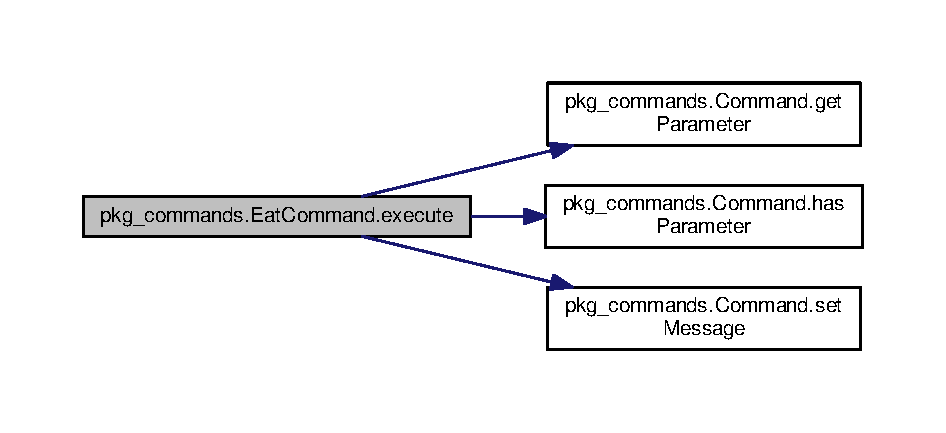
\includegraphics[width=350pt]{classpkg__commands_1_1EatCommand_a2a600f09891aa076b3f630293de965f4_cgraph}
\end{center}
\end{figure}




The documentation for this class was generated from the following file\-:\begin{DoxyCompactItemize}
\item 
pkg\-\_\-commands/\hyperlink{EatCommand_8java}{Eat\-Command.\-java}\end{DoxyCompactItemize}

\hypertarget{classGame}{\section{Game Class Reference}
\label{classGame}\index{Game@{Game}}
}


Main class used to instantiate other objects.  




Collaboration diagram for Game\-:
\nopagebreak
\begin{figure}[H]
\begin{center}
\leavevmode
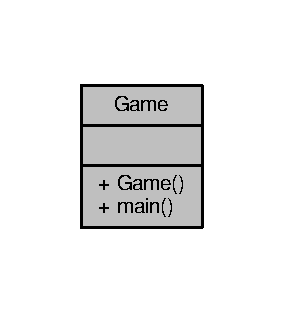
\includegraphics[width=136pt]{classGame__coll__graph}
\end{center}
\end{figure}
\subsection*{Public Member Functions}
\begin{DoxyCompactItemize}
\item 
\hyperlink{classGame_a2e034e53e9c032964ecd2a831b29a616}{Game} ()
\begin{DoxyCompactList}\small\item\em \hyperlink{classGame}{Game} class constructor. \end{DoxyCompactList}\end{DoxyCompactItemize}
\subsection*{Static Public Member Functions}
\begin{DoxyCompactItemize}
\item 
static void \hyperlink{classGame_ae52595a27ac1b327b05db2129ad81fca}{main} (String\mbox{[}$\,$\mbox{]} args)
\begin{DoxyCompactList}\small\item\em Main function. \end{DoxyCompactList}\end{DoxyCompactItemize}


\subsection{Detailed Description}
Main class used to instantiate other objects. 

\begin{DoxyAuthor}{Author}
Rémi N\-I\-C\-O\-L\-E 
\end{DoxyAuthor}


Definition at line \hyperlink{Game_8java_source_l00009}{9} of file \hyperlink{Game_8java_source}{Game.\-java}.



\subsection{Constructor \& Destructor Documentation}
\hypertarget{classGame_a2e034e53e9c032964ecd2a831b29a616}{\index{Game@{Game}!Game@{Game}}
\index{Game@{Game}!Game@{Game}}
\subsubsection[{Game}]{\setlength{\rightskip}{0pt plus 5cm}Game.\-Game (
\begin{DoxyParamCaption}
{}
\end{DoxyParamCaption}
)}}\label{classGame_a2e034e53e9c032964ecd2a831b29a616}


\hyperlink{classGame}{Game} class constructor. 



Definition at line \hyperlink{Game_8java_source_l00032}{32} of file \hyperlink{Game_8java_source}{Game.\-java}.



Referenced by \hyperlink{Game_8java_source_l00015}{main()}.


\begin{DoxyCode}
00032                    \{
00033         engine = \textcolor{keyword}{new} \hyperlink{classpkg__game_1_1GameEngine}{GameEngine}();
00034         gui = \textcolor{keyword}{new} \hyperlink{classpkg__game_1_1UserInterface}{UserInterface}(engine);
00035         engine.setGUI(gui);
00036     \}
\end{DoxyCode}


Here is the caller graph for this function\-:
\nopagebreak
\begin{figure}[H]
\begin{center}
\leavevmode
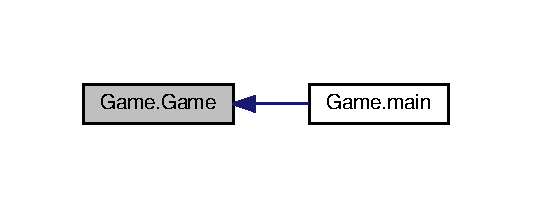
\includegraphics[width=256pt]{classGame_a2e034e53e9c032964ecd2a831b29a616_icgraph}
\end{center}
\end{figure}




\subsection{Member Function Documentation}
\hypertarget{classGame_ae52595a27ac1b327b05db2129ad81fca}{\index{Game@{Game}!main@{main}}
\index{main@{main}!Game@{Game}}
\subsubsection[{main}]{\setlength{\rightskip}{0pt plus 5cm}static void Game.\-main (
\begin{DoxyParamCaption}
\item[{String\mbox{[}$\,$\mbox{]}}]{args}
\end{DoxyParamCaption}
)\hspace{0.3cm}{\ttfamily [static]}}}\label{classGame_ae52595a27ac1b327b05db2129ad81fca}


Main function. 


\begin{DoxyParams}{Parameters}
{\em args} & Command line arguments \\
\hline
\end{DoxyParams}


Definition at line \hyperlink{Game_8java_source_l00015}{15} of file \hyperlink{Game_8java_source}{Game.\-java}.



References \hyperlink{Game_8java_source_l00032}{Game()}.


\begin{DoxyCode}
00015                                            \{
00016         \hyperlink{classGame}{Game} game = \textcolor{keyword}{new} \hyperlink{classGame_a2e034e53e9c032964ecd2a831b29a616}{Game}();
00017     \}
\end{DoxyCode}


Here is the call graph for this function\-:
\nopagebreak
\begin{figure}[H]
\begin{center}
\leavevmode
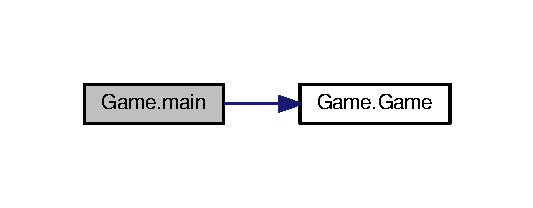
\includegraphics[width=256pt]{classGame_ae52595a27ac1b327b05db2129ad81fca_cgraph}
\end{center}
\end{figure}




The documentation for this class was generated from the following file\-:\begin{DoxyCompactItemize}
\item 
\hyperlink{Game_8java}{Game.\-java}\end{DoxyCompactItemize}

\hypertarget{classGameEngine}{\section{Game\-Engine Class Reference}
\label{classGameEngine}\index{Game\-Engine@{Game\-Engine}}
}


Class handling the gameplay for the game.  




Collaboration diagram for Game\-Engine\-:
\nopagebreak
\begin{figure}[H]
\begin{center}
\leavevmode
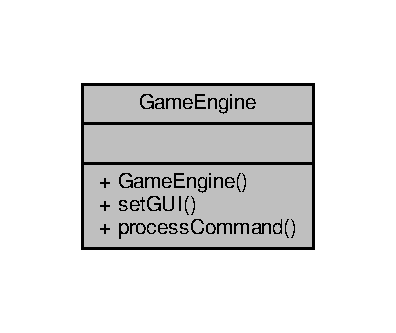
\includegraphics[height=550pt]{classGameEngine__coll__graph}
\end{center}
\end{figure}
\subsection*{Public Member Functions}
\begin{DoxyCompactItemize}
\item 
\hyperlink{classGameEngine_a9e8a92f5021a34293060f9aaff4005de}{Game\-Engine} ()
\begin{DoxyCompactList}\small\item\em \hyperlink{classGameEngine}{Game\-Engine} class constructor. \end{DoxyCompactList}\item 
void \hyperlink{classGameEngine_aec901a5b590b3cd204f196165da5dfb6}{set\-G\-U\-I} (\hyperlink{classUserInterface}{User\-Interface} user\-Interface)
\begin{DoxyCompactList}\small\item\em Setter for the gui field. \end{DoxyCompactList}\item 
void \hyperlink{classGameEngine_ad7133885f313fa99bca3bb7cb8272f64}{process\-Command} (String command\-Line)
\begin{DoxyCompactList}\small\item\em Process the command. \end{DoxyCompactList}\end{DoxyCompactItemize}
\subsection*{Package Attributes}
\begin{DoxyCompactItemize}
\item 
Array\-List$<$ \hyperlink{classRoom}{Room} $>$ \hyperlink{classGameEngine_ae5a2f252ec103e0630aebb8635341ea4}{game\-Rooms}
\begin{DoxyCompactList}\small\item\em A list of all the rooms in the game. \end{DoxyCompactList}\end{DoxyCompactItemize}
\subsection*{Private Member Functions}
\begin{DoxyCompactItemize}
\item 
void \hyperlink{classGameEngine_a9a2f3cb921bb19399e357bf14d26425b}{print\-Welcome} ()
\begin{DoxyCompactList}\small\item\em Welcome the user at the start of the game. \end{DoxyCompactList}\item 
\hyperlink{classRoom}{Room} \hyperlink{classGameEngine_a9410d92f7d0e6820059b1d07da364b09}{create\-Rooms} ()
\begin{DoxyCompactList}\small\item\em Create the rooms, link them and return the first \hyperlink{classRoom}{Room}. \end{DoxyCompactList}\item 
void \hyperlink{classGameEngine_a1f5fa36c5dfc36c9a963fe439afc057b}{end\-Game} (boolean winning)
\begin{DoxyCompactList}\small\item\em Print goodbye message and disable gui. \end{DoxyCompactList}\end{DoxyCompactItemize}
\subsection*{Private Attributes}
\begin{DoxyCompactItemize}
\item 
\hyperlink{classPlayer}{Player} \hyperlink{classGameEngine_a4666c6719428cc43014b30b305eeef5d}{player}
\begin{DoxyCompactList}\small\item\em \hyperlink{classPlayer}{Player} for the game. \end{DoxyCompactList}\item 
\hyperlink{classUserInterface}{User\-Interface} \hyperlink{classGameEngine_a2a7d0bb6183b3f3ef3ee2008926374a0}{gui}
\begin{DoxyCompactList}\small\item\em User interface for the game. \end{DoxyCompactList}\item 
int \hyperlink{classGameEngine_a308a9926d553d53cb4c56c28588f6c62}{help\-Count}
\begin{DoxyCompactList}\small\item\em Help query counter. \end{DoxyCompactList}\item 
int \hyperlink{classGameEngine_ad4ff8d760eced9c7b76cdeb0dc989975}{command\-Count\-Down}
\begin{DoxyCompactList}\small\item\em The command number limit of the game. \end{DoxyCompactList}\end{DoxyCompactItemize}


\subsection{Detailed Description}
Class handling the gameplay for the game. 

It takes care of rooms, parser, and room creations and command processing. \begin{DoxyAuthor}{Author}
Rémi N\-I\-C\-O\-L\-E 
\end{DoxyAuthor}


Definition at line \hyperlink{GameEngine_8java_source_l00013}{13} of file \hyperlink{GameEngine_8java_source}{Game\-Engine.\-java}.



\subsection{Constructor \& Destructor Documentation}
\hypertarget{classGameEngine_a9e8a92f5021a34293060f9aaff4005de}{\index{Game\-Engine@{Game\-Engine}!Game\-Engine@{Game\-Engine}}
\index{Game\-Engine@{Game\-Engine}!GameEngine@{Game\-Engine}}
\subsubsection[{Game\-Engine}]{\setlength{\rightskip}{0pt plus 5cm}Game\-Engine.\-Game\-Engine (
\begin{DoxyParamCaption}
{}
\end{DoxyParamCaption}
)}}\label{classGameEngine_a9e8a92f5021a34293060f9aaff4005de}


\hyperlink{classGameEngine}{Game\-Engine} class constructor. 



Definition at line \hyperlink{GameEngine_8java_source_l00047}{47} of file \hyperlink{GameEngine_8java_source}{Game\-Engine.\-java}.



References \hyperlink{GameEngine_8java_source_l00042}{command\-Count\-Down}, \hyperlink{GameEngine_8java_source_l00085}{create\-Rooms()}, \hyperlink{GameEngine_8java_source_l00023}{game\-Rooms}, \hyperlink{GameEngine_8java_source_l00036}{help\-Count}, and \hyperlink{GameEngine_8java_source_l00018}{player}.


\begin{DoxyCode}
00047                         \{
00048         \hyperlink{classGameEngine_ae5a2f252ec103e0630aebb8635341ea4}{gameRooms} = \textcolor{keyword}{new} ArrayList<Room>();
00049         \hyperlink{classGameEngine_a4666c6719428cc43014b30b305eeef5d}{player} = \textcolor{keyword}{new} \hyperlink{classPlayer}{Player}((javax.swing.JOptionPane.showInputDialog(\textcolor{stringliteral}{"What is your name"})
      .toLowerCase().equals(\textcolor{stringliteral}{"retard"}))? \textcolor{stringliteral}{"moron"} : \textcolor{stringliteral}{"retard"}, \hyperlink{classGameEngine_a9410d92f7d0e6820059b1d07da364b09}{createRooms}());
00050         javax.swing.JOptionPane.showMessageDialog(null, \textcolor{stringliteral}{"Whatever, I'll call you "} + player.getName() + \textcolor{stringliteral}{"."}
      );
00051         \hyperlink{classGameEngine_a308a9926d553d53cb4c56c28588f6c62}{helpCount} = 0;
00052         \hyperlink{classGameEngine_ad4ff8d760eced9c7b76cdeb0dc989975}{commandCountDown} = 42;
00053     \}
\end{DoxyCode}


Here is the call graph for this function\-:
\nopagebreak
\begin{figure}[H]
\begin{center}
\leavevmode
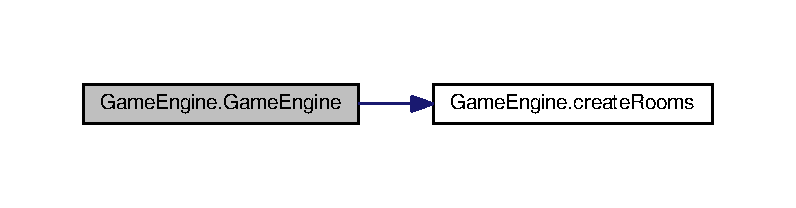
\includegraphics[width=350pt]{classGameEngine_a9e8a92f5021a34293060f9aaff4005de_cgraph}
\end{center}
\end{figure}




\subsection{Member Function Documentation}
\hypertarget{classGameEngine_a9410d92f7d0e6820059b1d07da364b09}{\index{Game\-Engine@{Game\-Engine}!create\-Rooms@{create\-Rooms}}
\index{create\-Rooms@{create\-Rooms}!GameEngine@{Game\-Engine}}
\subsubsection[{create\-Rooms}]{\setlength{\rightskip}{0pt plus 5cm}{\bf Room} Game\-Engine.\-create\-Rooms (
\begin{DoxyParamCaption}
{}
\end{DoxyParamCaption}
)\hspace{0.3cm}{\ttfamily [private]}}}\label{classGameEngine_a9410d92f7d0e6820059b1d07da364b09}


Create the rooms, link them and return the first \hyperlink{classRoom}{Room}. 

\begin{DoxyReturn}{Returns}
\hyperlink{classRoom}{Room} The first \hyperlink{classRoom}{Room} where the player should ba at start. 
\end{DoxyReturn}


Definition at line \hyperlink{GameEngine_8java_source_l00085}{85} of file \hyperlink{GameEngine_8java_source}{Game\-Engine.\-java}.



Referenced by \hyperlink{GameEngine_8java_source_l00047}{Game\-Engine()}.


\begin{DoxyCode}
00085                                \{
00086         \textcolor{comment}{// create the rooms}
00087         \hyperlink{classRoom}{Room} temperateBroadleaf = \textcolor{keyword}{new} \hyperlink{classRoom}{Room}(\textcolor{stringliteral}{"in temperate forest"}, \textcolor{stringliteral}{"temperatebroadleaf.jpg"});
00088         temperateBroadleaf.addItem(\textcolor{keyword}{new} \hyperlink{classItem}{Item}(\textcolor{stringliteral}{"wand"}, 3, \textcolor{stringliteral}{"just an ordinary wand"}));
00089 
00090         \hyperlink{classRoom}{Room} taiga = \textcolor{keyword}{new} \hyperlink{classRoom}{Room}(\textcolor{stringliteral}{"in a boreal forest"}, \textcolor{stringliteral}{"taiga.jpg"});
00091         taiga.addItem(\textcolor{keyword}{new} \hyperlink{classItem}{Item}(\textcolor{stringliteral}{"snowball"}, 1, \textcolor{stringliteral}{"some weirdly yellowy snowball"}));
00092         taiga.addItem(\textcolor{keyword}{new} \hyperlink{classItem}{Item}(\textcolor{stringliteral}{"bird"}, 6, \textcolor{stringliteral}{"a frozen inert black bird"}));
00093 
00094         \hyperlink{classRoom}{Room} alpineTundra = \textcolor{keyword}{new} \hyperlink{classRoom}{Room}(\textcolor{stringliteral}{"on an alpine mountain"}, \textcolor{stringliteral}{"alpinetundra.jpg"});
00095         alpineTundra.addItem(\textcolor{keyword}{new} \hyperlink{classItem}{Item}(\textcolor{stringliteral}{"rock"}, 15, \textcolor{stringliteral}{"a surprisingly solid magnificent rock"}));
00096         alpineTundra.addItem(\textcolor{keyword}{new} \hyperlink{classItem}{Item}(\textcolor{stringliteral}{"plank"}, 10, \textcolor{stringliteral}{"a plank of wood, maybe from a chalet"}));
00097         alpineTundra.addItem(\textcolor{keyword}{new} \hyperlink{classItem}{Item}(\textcolor{stringliteral}{"snowball"}, 1, \textcolor{stringliteral}{"a snowball. Yes, there is still snow in an alpine
       biome."}));
00098 
00099         \hyperlink{classRoom}{Room} steppe = \textcolor{keyword}{new} \hyperlink{classRoom}{Room}(\textcolor{stringliteral}{"on a vast grass plain"}, \textcolor{stringliteral}{"steppe.jpg"});
00100         steppe.addItem(\textcolor{keyword}{new} \hyperlink{classItem}{Item}(\textcolor{stringliteral}{"grass"}, 1, \textcolor{stringliteral}{"a tuft of yellowish grass. Looking at the grass made you
       look like stupid"}));
00101 
00102         \hyperlink{classRoom}{Room} cave = \textcolor{keyword}{new} \hyperlink{classRoom}{Room}(\textcolor{stringliteral}{"inside a dark cave"}, \textcolor{stringliteral}{"cave.jpg"});
00103         cave.addItem(\textcolor{keyword}{new} \hyperlink{classItem}{Item}(\textcolor{stringliteral}{"magiccookie"}, 3, \textcolor{stringliteral}{"a pretend magic cookie with mould on it, probably left
       there for many years. The use-by date has faded out. Why not eat it?"}));
00104 
00105         \hyperlink{classRoom}{Room} polarDesert = \textcolor{keyword}{new} \hyperlink{classRoom}{Room}(\textcolor{stringliteral}{"in a cold polar desert"}, \textcolor{stringliteral}{"polardesert.jpg"});
00106         polarDesert.addItem(\textcolor{keyword}{new} \hyperlink{classItem}{Item}(\textcolor{stringliteral}{"ice"}, 5, \textcolor{stringliteral}{"a little block of ice. But you don't have any drink"}));
00107 
00108         \hyperlink{classRoom}{Room} xericShrublands = \textcolor{keyword}{new} \hyperlink{classRoom}{Room}(\textcolor{stringliteral}{"in a sand desert"}, \textcolor{stringliteral}{"xericshrublands.jpg"});
00109         xericShrublands.addItem(\textcolor{keyword}{new} \hyperlink{classItem}{Item}(\textcolor{stringliteral}{"shrub"}, 10, \textcolor{stringliteral}{"a spicky shrub. Useful if you want to make a
       shruberry"}));
00110 
00111         \hyperlink{classRoom}{Room} savanna = \textcolor{keyword}{new} \hyperlink{classRoom}{Room}(\textcolor{stringliteral}{"in a savanna"}, \textcolor{stringliteral}{"savanna.jpg"});
00112         savanna.addItem(\textcolor{keyword}{new} \hyperlink{classItem}{Item}(\textcolor{stringliteral}{"elephant"}, 1000, \textcolor{stringliteral}{"a huge elephant looking at you, dazed. I bet he's
       smarter than you"}));
00113         savanna.addItem(\textcolor{keyword}{new} \hyperlink{classItem}{Item}(\textcolor{stringliteral}{"grass"}, 1, \textcolor{stringliteral}{"a tuft of yellowish grass. You may have other things to
       do instead of looking at that"}));
00114 
00115         \textcolor{comment}{// initialise room exits}
00116         temperateBroadleaf.setExit(\textcolor{stringliteral}{"east"}, taiga);
00117         temperateBroadleaf.setExit(\textcolor{stringliteral}{"south"}, steppe);
00118 
00119         taiga.setExit(\textcolor{stringliteral}{"west"}, temperateBroadleaf);
00120         taiga.setExit(\textcolor{stringliteral}{"east"}, alpineTundra);
00121         taiga.setExit(\textcolor{stringliteral}{"south"}, cave);
00122 
00123         alpineTundra.setExit(\textcolor{stringliteral}{"west"}, taiga);
00124         alpineTundra.setExit(\textcolor{stringliteral}{"south"}, polarDesert);
00125 
00126         steppe.setExit(\textcolor{stringliteral}{"north"}, temperateBroadleaf);
00127         steppe.setExit(\textcolor{stringliteral}{"east"}, cave);
00128         steppe.setExit(\textcolor{stringliteral}{"south"}, xericShrublands);
00129 
00130         cave.setExit(\textcolor{stringliteral}{"north"}, taiga);
00131         cave.setExit(\textcolor{stringliteral}{"south"}, savanna);
00132         cave.setExit(\textcolor{stringliteral}{"east"}, polarDesert);
00133         cave.setExit(\textcolor{stringliteral}{"west"}, steppe);
00134 
00135         \textcolor{comment}{// Trap Door}
00136         \textcolor{comment}{// polarDesert.setExit("north", alpineTundra);}
00137         polarDesert.setExit(\textcolor{stringliteral}{"west"}, cave);
00138 
00139         xericShrublands.setExit(\textcolor{stringliteral}{"north"}, steppe);
00140         xericShrublands.setExit(\textcolor{stringliteral}{"east"}, savanna);
00141 
00142         savanna.setExit(\textcolor{stringliteral}{"north"}, cave);
00143         savanna.setExit(\textcolor{stringliteral}{"west"}, xericShrublands);
00144 
00145         \hyperlink{classRoom}{Room} randomRoom = \textcolor{keyword}{new} \hyperlink{classRoom}{Room}(\textcolor{stringliteral}{""}, \textcolor{stringliteral}{""});
00146 
00147         polarDesert.setExit(\textcolor{stringliteral}{"south"}, randomRoom);
00148         savanna.setExit(\textcolor{stringliteral}{"east"}, randomRoom);
00149 
00150         gameRooms.add(randomRoom);
00151         gameRooms.add(temperateBroadleaf);
00152         gameRooms.add(taiga);
00153         gameRooms.add(alpineTundra);
00154         gameRooms.add(steppe);
00155         gameRooms.add(cave);
00156         gameRooms.add(polarDesert);
00157         gameRooms.add(xericShrublands);
00158         gameRooms.add(savanna);
00159 
00160         \textcolor{keywordflow}{return} temperateBroadleaf;
00161     \}
\end{DoxyCode}


Here is the caller graph for this function\-:
\nopagebreak
\begin{figure}[H]
\begin{center}
\leavevmode
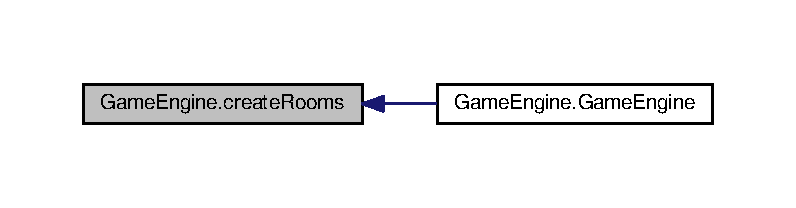
\includegraphics[width=350pt]{classGameEngine_a9410d92f7d0e6820059b1d07da364b09_icgraph}
\end{center}
\end{figure}


\hypertarget{classGameEngine_a1f5fa36c5dfc36c9a963fe439afc057b}{\index{Game\-Engine@{Game\-Engine}!end\-Game@{end\-Game}}
\index{end\-Game@{end\-Game}!GameEngine@{Game\-Engine}}
\subsubsection[{end\-Game}]{\setlength{\rightskip}{0pt plus 5cm}void Game\-Engine.\-end\-Game (
\begin{DoxyParamCaption}
\item[{boolean}]{winning}
\end{DoxyParamCaption}
)\hspace{0.3cm}{\ttfamily [private]}}}\label{classGameEngine_a1f5fa36c5dfc36c9a963fe439afc057b}


Print goodbye message and disable gui. 


\begin{DoxyParams}{Parameters}
{\em winning} & Equals to true if the player won \\
\hline
\end{DoxyParams}


Definition at line \hyperlink{GameEngine_8java_source_l00213}{213} of file \hyperlink{GameEngine_8java_source}{Game\-Engine.\-java}.



Referenced by \hyperlink{GameEngine_8java_source_l00167}{process\-Command()}.


\begin{DoxyCode}
00213                                           \{
00214         gui.println(\textcolor{stringliteral}{"Thank you for playing. Good bye. By the way, you "}
00215                 + ((winning)? \textcolor{stringliteral}{"won"} : \textcolor{stringliteral}{"lost"}) + \textcolor{stringliteral}{"."});
00216         gui.enable(\textcolor{keyword}{false});
00217     \}
\end{DoxyCode}


Here is the caller graph for this function\-:
\nopagebreak
\begin{figure}[H]
\begin{center}
\leavevmode
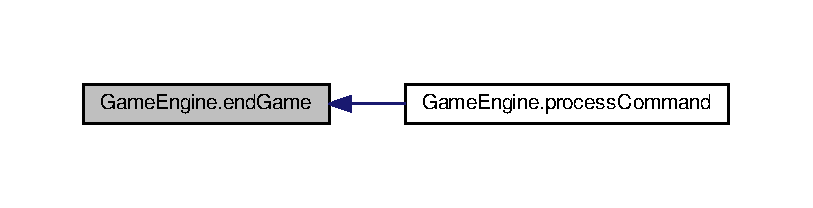
\includegraphics[width=350pt]{classGameEngine_a1f5fa36c5dfc36c9a963fe439afc057b_icgraph}
\end{center}
\end{figure}


\hypertarget{classGameEngine_a9a2f3cb921bb19399e357bf14d26425b}{\index{Game\-Engine@{Game\-Engine}!print\-Welcome@{print\-Welcome}}
\index{print\-Welcome@{print\-Welcome}!GameEngine@{Game\-Engine}}
\subsubsection[{print\-Welcome}]{\setlength{\rightskip}{0pt plus 5cm}void Game\-Engine.\-print\-Welcome (
\begin{DoxyParamCaption}
{}
\end{DoxyParamCaption}
)\hspace{0.3cm}{\ttfamily [private]}}}\label{classGameEngine_a9a2f3cb921bb19399e357bf14d26425b}


Welcome the user at the start of the game. 



Definition at line \hyperlink{GameEngine_8java_source_l00068}{68} of file \hyperlink{GameEngine_8java_source}{Game\-Engine.\-java}.



Referenced by \hyperlink{GameEngine_8java_source_l00059}{set\-G\-U\-I()}.


\begin{DoxyCode}
00068                                 \{
00069         gui.println(\textcolor{stringliteral}{"Greetings human."});
00070         gui.println(\textcolor{stringliteral}{"I see the assassins have failed. Too bad..."});
00071         gui.println(\textcolor{stringliteral}{"You know what they say: if you want something done, do it yourself."});
00072         gui.println(\textcolor{stringliteral}{"At least I can see that you don't remember anything. At last something that I can take
       advantage of."});
00073         gui.println(\textcolor{stringliteral}{"That was predictable, human minds are weak."});
00074         gui.println(\textcolor{stringliteral}{"\(\backslash\)nBecause you're stupid, I will describe you everything that will be around us."});
00075         gui.println(\textcolor{stringliteral}{"Who knows ? Maybe you can turn into something useful. One day. Maybe."});
00076         gui.println(\textcolor{stringliteral}{"\(\backslash\)nBeware: Death is coming!\(\backslash\)n"});
00077         gui.println(player.getCurrentRoom().getLongDescription());
00078         gui.showImage(player.getCurrentRoom().getImageName());
00079     \}
\end{DoxyCode}


Here is the caller graph for this function\-:
\nopagebreak
\begin{figure}[H]
\begin{center}
\leavevmode
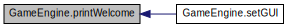
\includegraphics[width=350pt]{classGameEngine_a9a2f3cb921bb19399e357bf14d26425b_icgraph}
\end{center}
\end{figure}


\hypertarget{classGameEngine_ad7133885f313fa99bca3bb7cb8272f64}{\index{Game\-Engine@{Game\-Engine}!process\-Command@{process\-Command}}
\index{process\-Command@{process\-Command}!GameEngine@{Game\-Engine}}
\subsubsection[{process\-Command}]{\setlength{\rightskip}{0pt plus 5cm}void Game\-Engine.\-process\-Command (
\begin{DoxyParamCaption}
\item[{String}]{command\-Line}
\end{DoxyParamCaption}
)}}\label{classGameEngine_ad7133885f313fa99bca3bb7cb8272f64}


Process the command. 


\begin{DoxyParams}{Parameters}
{\em command\-Line} & The command to process. \\
\hline
\end{DoxyParams}


Definition at line \hyperlink{GameEngine_8java_source_l00167}{167} of file \hyperlink{GameEngine_8java_source}{Game\-Engine.\-java}.



References \hyperlink{GameEngine_8java_source_l00042}{command\-Count\-Down}, \hyperlink{GameEngine_8java_source_l00213}{end\-Game()}, \hyperlink{Player_8java_source_l00089}{Player.\-get\-Current\-Room()}, \hyperlink{GameEngine_8java_source_l00028}{gui}, \hyperlink{GameEngine_8java_source_l00018}{player}, and \hyperlink{UserInterface_8java_source_l00073}{User\-Interface.\-println()}.


\begin{DoxyCode}
00167                                                    \{
00168         gui.println(\textcolor{stringliteral}{"\(\backslash\)n"} + commandLine + \textcolor{stringliteral}{"\(\backslash\)n"});
00169         \hyperlink{classCommand}{Command} command = Parser.getCommand(commandLine);
00170 
00171         \textcolor{keywordflow}{if}(command == null) \{
00172             gui.println(\textcolor{stringliteral}{"I don't know what you mean..."});
00173             \textcolor{keywordflow}{return};
00174         \}
00175 
00176         gui.setCommandsLeft(--\hyperlink{classGameEngine_ad4ff8d760eced9c7b76cdeb0dc989975}{commandCountDown});
00177 
00178         \textcolor{keywordflow}{try} \{
00179             \textcolor{keywordtype}{boolean} quit = command.execute(\hyperlink{classGameEngine_a4666c6719428cc43014b30b305eeef5d}{player});
00180 
00181             \textcolor{keywordflow}{if}(command.hasMessage())
00182                 \hyperlink{classGameEngine_a2a7d0bb6183b3f3ef3ee2008926374a0}{gui}.\hyperlink{classUserInterface_a79f606b4b1f5d1523e50eea00039ed94}{println}(command.getMessage());
00183             \textcolor{comment}{// If we can cast the command into a GoCommand}
00184             \textcolor{comment}{// Or if it is the test command}
00185             \textcolor{keywordflow}{if}(\hyperlink{classGoCommand}{GoCommand}.class.isInstance(command) || command.getClass().equals(
      \hyperlink{classTestCommand}{TestCommand}.class)) \{
00186                 \textcolor{comment}{// The game image is reloaded}
00187                 \textcolor{keywordflow}{if}(\hyperlink{classGameEngine_a4666c6719428cc43014b30b305eeef5d}{player}.\hyperlink{classPlayer_a3a3107df50fc4e35e8c0f46c3f776ce6}{getCurrentRoom}().getImageName() != null) \{
00188                     gui.showImage(player.getCurrentRoom().getImageName());
00189                 \}
00190             \}
00191 
00192             \textcolor{keywordflow}{if}(quit) \{
00193                 \hyperlink{classGameEngine_a1f5fa36c5dfc36c9a963fe439afc057b}{endGame}(\textcolor{keyword}{false});
00194             \}
00195         \} \textcolor{keywordflow}{catch}(\hyperlink{classNoArgumentException}{NoArgumentException} e) \{
00196             gui.println(e.getMessage());
00197         \} \textcolor{keywordflow}{catch}(\hyperlink{classIllegalArgumentException}{IllegalArgumentException} e) \{
00198             gui.println(e.getMessage());
00199         \} \textcolor{keywordflow}{catch}(\hyperlink{classUnauthorizedException}{UnauthorizedException} e) \{
00200             gui.println(e.getMessage());
00201         \}
00202 
00203         \textcolor{keywordflow}{if}(\hyperlink{classGameEngine_ad4ff8d760eced9c7b76cdeb0dc989975}{commandCountDown} == 0) \{
00204             \hyperlink{classGameEngine_a1f5fa36c5dfc36c9a963fe439afc057b}{endGame}(\textcolor{keyword}{false});
00205         \}
00206 
00207     \}
\end{DoxyCode}


Here is the call graph for this function\-:
\nopagebreak
\begin{figure}[H]
\begin{center}
\leavevmode
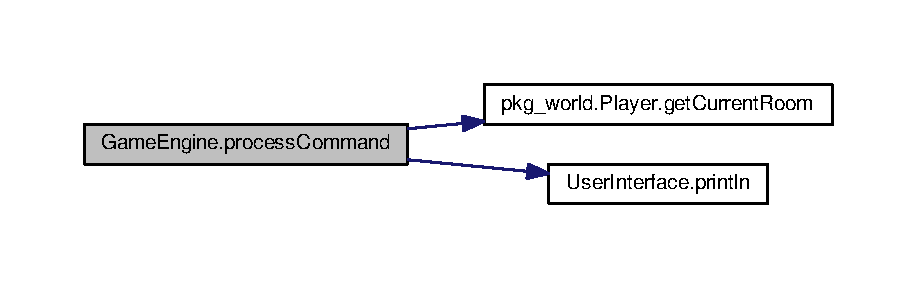
\includegraphics[width=350pt]{classGameEngine_ad7133885f313fa99bca3bb7cb8272f64_cgraph}
\end{center}
\end{figure}


\hypertarget{classGameEngine_aec901a5b590b3cd204f196165da5dfb6}{\index{Game\-Engine@{Game\-Engine}!set\-G\-U\-I@{set\-G\-U\-I}}
\index{set\-G\-U\-I@{set\-G\-U\-I}!GameEngine@{Game\-Engine}}
\subsubsection[{set\-G\-U\-I}]{\setlength{\rightskip}{0pt plus 5cm}void Game\-Engine.\-set\-G\-U\-I (
\begin{DoxyParamCaption}
\item[{{\bf User\-Interface}}]{user\-Interface}
\end{DoxyParamCaption}
)}}\label{classGameEngine_aec901a5b590b3cd204f196165da5dfb6}


Setter for the gui field. 


\begin{DoxyParams}{Parameters}
{\em user\-Interface} & The user interface to set \\
\hline
\end{DoxyParams}


Definition at line \hyperlink{GameEngine_8java_source_l00059}{59} of file \hyperlink{GameEngine_8java_source}{Game\-Engine.\-java}.



References \hyperlink{GameEngine_8java_source_l00042}{command\-Count\-Down}, \hyperlink{GameEngine_8java_source_l00028}{gui}, and \hyperlink{GameEngine_8java_source_l00068}{print\-Welcome()}.


\begin{DoxyCode}
00059                                                     \{
00060         \hyperlink{classGameEngine_a2a7d0bb6183b3f3ef3ee2008926374a0}{gui} = userInterface;
00061         gui.setCommandsLeft(\hyperlink{classGameEngine_ad4ff8d760eced9c7b76cdeb0dc989975}{commandCountDown});
00062         \hyperlink{classGameEngine_a9a2f3cb921bb19399e357bf14d26425b}{printWelcome}();
00063     \}
\end{DoxyCode}


Here is the call graph for this function\-:
\nopagebreak
\begin{figure}[H]
\begin{center}
\leavevmode
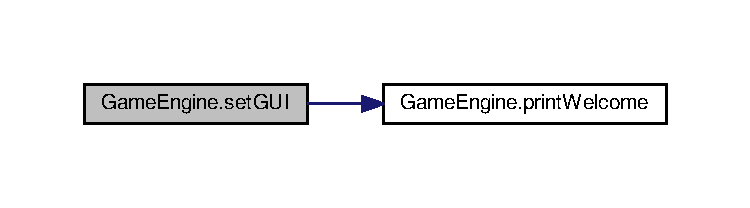
\includegraphics[width=350pt]{classGameEngine_aec901a5b590b3cd204f196165da5dfb6_cgraph}
\end{center}
\end{figure}




\subsection{Member Data Documentation}
\hypertarget{classGameEngine_ad4ff8d760eced9c7b76cdeb0dc989975}{\index{Game\-Engine@{Game\-Engine}!command\-Count\-Down@{command\-Count\-Down}}
\index{command\-Count\-Down@{command\-Count\-Down}!GameEngine@{Game\-Engine}}
\subsubsection[{command\-Count\-Down}]{\setlength{\rightskip}{0pt plus 5cm}int Game\-Engine.\-command\-Count\-Down\hspace{0.3cm}{\ttfamily [private]}}}\label{classGameEngine_ad4ff8d760eced9c7b76cdeb0dc989975}


The command number limit of the game. 

It is initially equals to 42 

Definition at line \hyperlink{GameEngine_8java_source_l00042}{42} of file \hyperlink{GameEngine_8java_source}{Game\-Engine.\-java}.



Referenced by \hyperlink{GameEngine_8java_source_l00047}{Game\-Engine()}, \hyperlink{GameEngine_8java_source_l00167}{process\-Command()}, and \hyperlink{GameEngine_8java_source_l00059}{set\-G\-U\-I()}.

\hypertarget{classGameEngine_ae5a2f252ec103e0630aebb8635341ea4}{\index{Game\-Engine@{Game\-Engine}!game\-Rooms@{game\-Rooms}}
\index{game\-Rooms@{game\-Rooms}!GameEngine@{Game\-Engine}}
\subsubsection[{game\-Rooms}]{\setlength{\rightskip}{0pt plus 5cm}Array\-List$<${\bf Room}$>$ Game\-Engine.\-game\-Rooms\hspace{0.3cm}{\ttfamily [package]}}}\label{classGameEngine_ae5a2f252ec103e0630aebb8635341ea4}


A list of all the rooms in the game. 



Definition at line \hyperlink{GameEngine_8java_source_l00023}{23} of file \hyperlink{GameEngine_8java_source}{Game\-Engine.\-java}.



Referenced by \hyperlink{GameEngine_8java_source_l00047}{Game\-Engine()}.

\hypertarget{classGameEngine_a2a7d0bb6183b3f3ef3ee2008926374a0}{\index{Game\-Engine@{Game\-Engine}!gui@{gui}}
\index{gui@{gui}!GameEngine@{Game\-Engine}}
\subsubsection[{gui}]{\setlength{\rightskip}{0pt plus 5cm}{\bf User\-Interface} Game\-Engine.\-gui\hspace{0.3cm}{\ttfamily [private]}}}\label{classGameEngine_a2a7d0bb6183b3f3ef3ee2008926374a0}


User interface for the game. 



Definition at line \hyperlink{GameEngine_8java_source_l00028}{28} of file \hyperlink{GameEngine_8java_source}{Game\-Engine.\-java}.



Referenced by \hyperlink{GameEngine_8java_source_l00167}{process\-Command()}, and \hyperlink{GameEngine_8java_source_l00059}{set\-G\-U\-I()}.

\hypertarget{classGameEngine_a308a9926d553d53cb4c56c28588f6c62}{\index{Game\-Engine@{Game\-Engine}!help\-Count@{help\-Count}}
\index{help\-Count@{help\-Count}!GameEngine@{Game\-Engine}}
\subsubsection[{help\-Count}]{\setlength{\rightskip}{0pt plus 5cm}int Game\-Engine.\-help\-Count\hspace{0.3cm}{\ttfamily [private]}}}\label{classGameEngine_a308a9926d553d53cb4c56c28588f6c62}


Help query counter. 

It is equal to 0 if the user did not asked for help, 1 if the user asked once the help and 2 if the user asked twice or more for the help 

Definition at line \hyperlink{GameEngine_8java_source_l00036}{36} of file \hyperlink{GameEngine_8java_source}{Game\-Engine.\-java}.



Referenced by \hyperlink{GameEngine_8java_source_l00047}{Game\-Engine()}.

\hypertarget{classGameEngine_a4666c6719428cc43014b30b305eeef5d}{\index{Game\-Engine@{Game\-Engine}!player@{player}}
\index{player@{player}!GameEngine@{Game\-Engine}}
\subsubsection[{player}]{\setlength{\rightskip}{0pt plus 5cm}{\bf Player} Game\-Engine.\-player\hspace{0.3cm}{\ttfamily [private]}}}\label{classGameEngine_a4666c6719428cc43014b30b305eeef5d}


\hyperlink{classPlayer}{Player} for the game. 



Definition at line \hyperlink{GameEngine_8java_source_l00018}{18} of file \hyperlink{GameEngine_8java_source}{Game\-Engine.\-java}.



Referenced by \hyperlink{GameEngine_8java_source_l00047}{Game\-Engine()}, and \hyperlink{GameEngine_8java_source_l00167}{process\-Command()}.



The documentation for this class was generated from the following file\-:\begin{DoxyCompactItemize}
\item 
\hyperlink{GameEngine_8java}{Game\-Engine.\-java}\end{DoxyCompactItemize}

\hypertarget{classpkg__commands_1_1GoCommand}{\section{pkg\-\_\-commands.\-Go\-Command Class Reference}
\label{classpkg__commands_1_1GoCommand}\index{pkg\-\_\-commands.\-Go\-Command@{pkg\-\_\-commands.\-Go\-Command}}
}


Inheritance diagram for pkg\-\_\-commands.\-Go\-Command\-:
\nopagebreak
\begin{figure}[H]
\begin{center}
\leavevmode
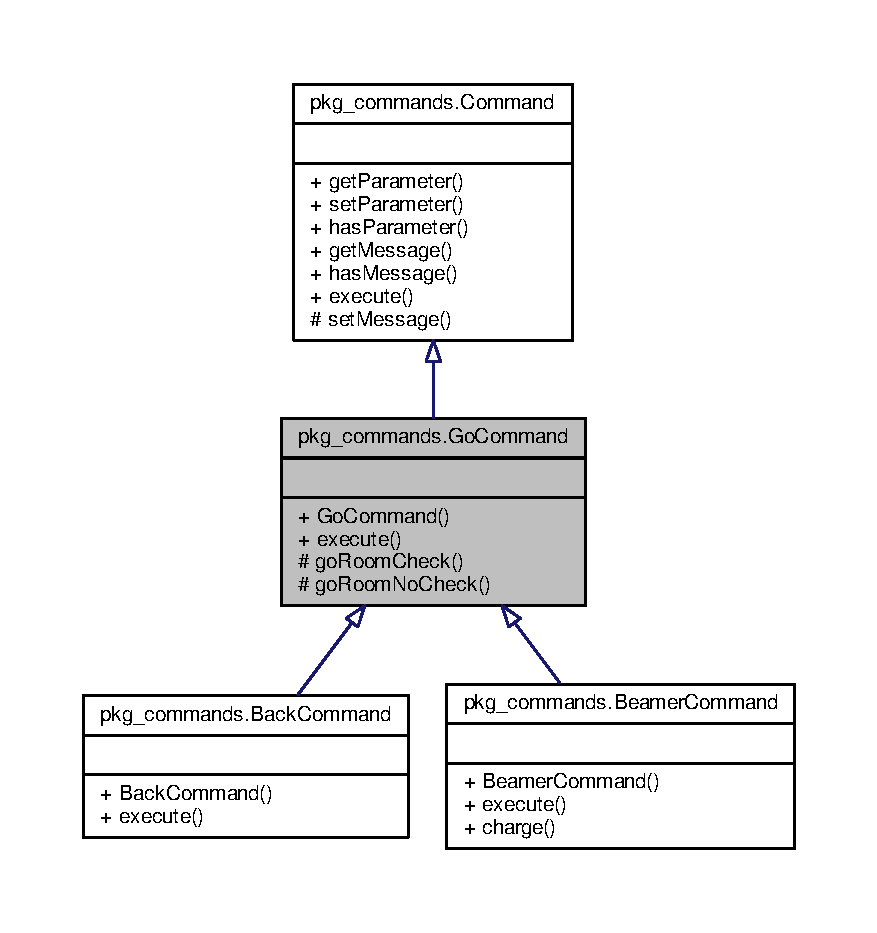
\includegraphics[width=350pt]{classpkg__commands_1_1GoCommand__inherit__graph}
\end{center}
\end{figure}


Collaboration diagram for pkg\-\_\-commands.\-Go\-Command\-:
\nopagebreak
\begin{figure}[H]
\begin{center}
\leavevmode
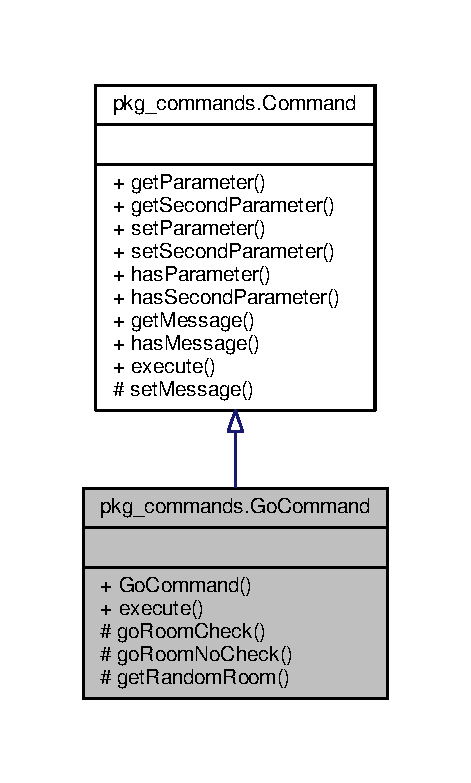
\includegraphics[width=226pt]{classpkg__commands_1_1GoCommand__coll__graph}
\end{center}
\end{figure}
\subsection*{Public Member Functions}
\begin{DoxyCompactItemize}
\item 
\hyperlink{classpkg__commands_1_1GoCommand_af87b7ac858440df2c3d850c89441f4c7}{Go\-Command} ()
\item 
boolean \hyperlink{classpkg__commands_1_1GoCommand_a82e9a64a0fac612f788060a90c83f9b1}{execute} (\hyperlink{classpkg__world_1_1Player}{Player} player)  throws No\-Argument\-Exception,pkg\-\_\-exceptions.\-Illegal\-Argument\-Exception,\-Unauthorized\-Exception 
\end{DoxyCompactItemize}
\subsection*{Protected Member Functions}
\begin{DoxyCompactItemize}
\item 
void \hyperlink{classpkg__commands_1_1GoCommand_acbf1aa81fa5b1aef7cafb8b4e3ace3a9}{go\-Room\-Check} (\hyperlink{classpkg__world_1_1Room}{Room} room, \hyperlink{classpkg__world_1_1Player}{Player} player, boolean back)  throws pkg\-\_\-exceptions.\-Illegal\-Argument\-Exception,\-Unauthorized\-Exception 
\item 
void \hyperlink{classpkg__commands_1_1GoCommand_a210afbc5f3ef34d3ad5759d853c8f8c2}{go\-Room\-No\-Check} (\hyperlink{classpkg__world_1_1Room}{Room} room, \hyperlink{classpkg__world_1_1Player}{Player} player, boolean back)  throws pkg\-\_\-exceptions.\-Illegal\-Argument\-Exception 
\item 
\hyperlink{classpkg__world_1_1Room}{Room} \hyperlink{classpkg__commands_1_1GoCommand_ae9ef6c18b0cbd0e0104261bdedf9a9d7}{get\-Random\-Room} ()
\end{DoxyCompactItemize}


\subsection{Detailed Description}
class \hyperlink{classpkg__commands_1_1GoCommand}{Go\-Command} used to make the player go to a given Room. \begin{DoxyAuthor}{Author}
Rémi Nicole 
\end{DoxyAuthor}


Definition at line \hyperlink{GoCommand_8java_source_l00015}{15} of file \hyperlink{GoCommand_8java_source}{Go\-Command.\-java}.



\subsection{Constructor \& Destructor Documentation}
\hypertarget{classpkg__commands_1_1GoCommand_af87b7ac858440df2c3d850c89441f4c7}{\index{pkg\-\_\-commands\-::\-Go\-Command@{pkg\-\_\-commands\-::\-Go\-Command}!Go\-Command@{Go\-Command}}
\index{Go\-Command@{Go\-Command}!pkg_commands::GoCommand@{pkg\-\_\-commands\-::\-Go\-Command}}
\subsubsection[{Go\-Command}]{\setlength{\rightskip}{0pt plus 5cm}pkg\-\_\-commands.\-Go\-Command.\-Go\-Command (
\begin{DoxyParamCaption}
{}
\end{DoxyParamCaption}
)}}\label{classpkg__commands_1_1GoCommand_af87b7ac858440df2c3d850c89441f4c7}
Constructor for \hyperlink{classpkg__commands_1_1GoCommand}{Go\-Command}. 

Definition at line \hyperlink{GoCommand_8java_source_l00020}{20} of file \hyperlink{GoCommand_8java_source}{Go\-Command.\-java}.


\begin{DoxyCode}
00020                        \{
00021 
00022     \}
\end{DoxyCode}


\subsection{Member Function Documentation}
\hypertarget{classpkg__commands_1_1GoCommand_a82e9a64a0fac612f788060a90c83f9b1}{\index{pkg\-\_\-commands\-::\-Go\-Command@{pkg\-\_\-commands\-::\-Go\-Command}!execute@{execute}}
\index{execute@{execute}!pkg_commands::GoCommand@{pkg\-\_\-commands\-::\-Go\-Command}}
\subsubsection[{execute}]{\setlength{\rightskip}{0pt plus 5cm}boolean pkg\-\_\-commands.\-Go\-Command.\-execute (
\begin{DoxyParamCaption}
\item[{{\bf Player}}]{player}
\end{DoxyParamCaption}
) throws {\bf No\-Argument\-Exception},{\bf pkg\-\_\-exceptions.\-Illegal\-Argument\-Exception},{\bf Unauthorized\-Exception}}}\label{classpkg__commands_1_1GoCommand_a82e9a64a0fac612f788060a90c83f9b1}
Make the player go to the Room through it's direction in the parameter field. 
\begin{DoxyParams}{Parameters}
{\em player} & The player that called this command \\
\hline
\end{DoxyParams}

\begin{DoxyExceptions}{Exceptions}
{\em No\-Argument\-Exception} & When the user typed the command without parameter \\
\hline
{\em Illegal\-Argument\-Exception} & When the user typed a parameter other than an available exit direction \\
\hline
{\em Unauthorized\-Exception} & When the user isn't allowed to go to the given Room \\
\hline
\end{DoxyExceptions}
\begin{DoxyReturn}{Returns}
False because it is not the quit command 
\end{DoxyReturn}


Definition at line \hyperlink{GoCommand_8java_source_l00032}{32} of file \hyperlink{GoCommand_8java_source}{Go\-Command.\-java}.



References \hyperlink{Command_8java_source_l00041}{pkg\-\_\-commands.\-Command.\-get\-Parameter()}, \hyperlink{GoCommand_8java_source_l00087}{pkg\-\_\-commands.\-Go\-Command.\-get\-Random\-Room()}, \hyperlink{GoCommand_8java_source_l00056}{pkg\-\_\-commands.\-Go\-Command.\-go\-Room\-Check()}, \hyperlink{GoCommand_8java_source_l00071}{pkg\-\_\-commands.\-Go\-Command.\-go\-Room\-No\-Check()}, \hyperlink{Command_8java_source_l00073}{pkg\-\_\-commands.\-Command.\-has\-Parameter()}, and \hyperlink{Command_8java_source_l00089}{pkg\-\_\-commands.\-Command.\-set\-Message()}.


\begin{DoxyCode}
00032                                                                                                            
                              \{
00033         \hyperlink{classpkg__commands_1_1Command_ae210ff216fe908b111ba1c988a963d13}{setMessage}(\textcolor{stringliteral}{""});
00034         \textcolor{comment}{// Check if it is the random Room (which is the first room in the gamesRoom GameEngine ArrayList)}
00035         \textcolor{keywordflow}{if}(player.getCurrentRoom() != GameEngine.getRooms().\textcolor{keyword}{get}(0)) \{
00036             \textcolor{keywordflow}{if}(\hyperlink{classpkg__commands_1_1Command_a02af95ab3f1898a66259ab7c177b6998}{hasParameter}()) \{
00037                 \hyperlink{classpkg__commands_1_1GoCommand_acbf1aa81fa5b1aef7cafb8b4e3ace3a9}{goRoomCheck}(player.getCurrentRoom().getExit(
      \hyperlink{classpkg__commands_1_1Command_a41c92d445be73ea9d62320c65efb8434}{getParameter}()), player, \textcolor{keyword}{false});
00038             \} \textcolor{keywordflow}{else} \{
00039                 \textcolor{keywordflow}{throw} \textcolor{keyword}{new} \hyperlink{classpkg__exceptions_1_1NoArgumentException}{NoArgumentException}(\textcolor{stringliteral}{"If you were clever, I would have thought
       that it was a existential question.\(\backslash\)nBut that is not the case and I cannot allow you to go nowhere"});
00040             \}
00041         \} \textcolor{keywordflow}{else} \{
00042             \hyperlink{classpkg__commands_1_1Command_ae210ff216fe908b111ba1c988a963d13}{setMessage}(\textcolor{stringliteral}{"Geronimoooo !\(\backslash\)n"});
00043             \hyperlink{classpkg__commands_1_1GoCommand_a210afbc5f3ef34d3ad5759d853c8f8c2}{goRoomNoCheck}(\hyperlink{classpkg__commands_1_1GoCommand_ae9ef6c18b0cbd0e0104261bdedf9a9d7}{getRandomRoom}(), player, \textcolor{keyword}{false});
00044         \}
00045         \textcolor{keywordflow}{return} \textcolor{keyword}{false};
00046     \}
\end{DoxyCode}


Here is the call graph for this function\-:
\nopagebreak
\begin{figure}[H]
\begin{center}
\leavevmode
\includegraphics[width=350pt]{classpkg__commands_1_1GoCommand_a82e9a64a0fac612f788060a90c83f9b1_cgraph}
\end{center}
\end{figure}


\hypertarget{classpkg__commands_1_1GoCommand_ae9ef6c18b0cbd0e0104261bdedf9a9d7}{\index{pkg\-\_\-commands\-::\-Go\-Command@{pkg\-\_\-commands\-::\-Go\-Command}!get\-Random\-Room@{get\-Random\-Room}}
\index{get\-Random\-Room@{get\-Random\-Room}!pkg_commands::GoCommand@{pkg\-\_\-commands\-::\-Go\-Command}}
\subsubsection[{get\-Random\-Room}]{\setlength{\rightskip}{0pt plus 5cm}{\bf Room} pkg\-\_\-commands.\-Go\-Command.\-get\-Random\-Room (
\begin{DoxyParamCaption}
{}
\end{DoxyParamCaption}
)\hspace{0.3cm}{\ttfamily [protected]}}}\label{classpkg__commands_1_1GoCommand_ae9ef6c18b0cbd0e0104261bdedf9a9d7}
Get a random room from the Game\-Engin list or Room. \begin{DoxyReturn}{Returns}
A random room 
\end{DoxyReturn}


Definition at line \hyperlink{GoCommand_8java_source_l00087}{87} of file \hyperlink{GoCommand_8java_source}{Go\-Command.\-java}.



Referenced by \hyperlink{GoCommand_8java_source_l00032}{pkg\-\_\-commands.\-Go\-Command.\-execute()}.


\begin{DoxyCode}
00087                                    \{
00088         \textcolor{keywordflow}{return} GameEngine.getRooms().\textcolor{keyword}{get}((\textcolor{keyword}{new} Random()).nextInt(GameEngine.getRooms().size() - 1) + 1);
00089     \}
\end{DoxyCode}


Here is the caller graph for this function\-:
\nopagebreak
\begin{figure}[H]
\begin{center}
\leavevmode
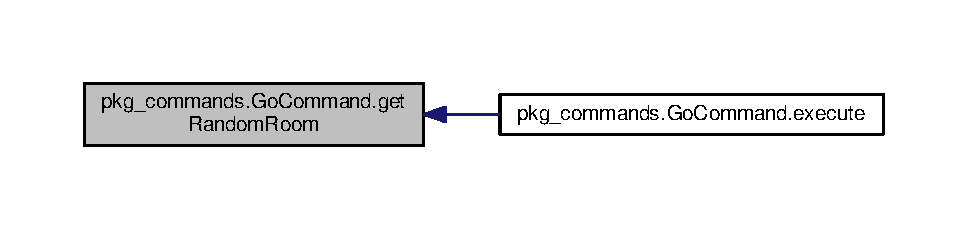
\includegraphics[width=350pt]{classpkg__commands_1_1GoCommand_ae9ef6c18b0cbd0e0104261bdedf9a9d7_icgraph}
\end{center}
\end{figure}


\hypertarget{classpkg__commands_1_1GoCommand_acbf1aa81fa5b1aef7cafb8b4e3ace3a9}{\index{pkg\-\_\-commands\-::\-Go\-Command@{pkg\-\_\-commands\-::\-Go\-Command}!go\-Room\-Check@{go\-Room\-Check}}
\index{go\-Room\-Check@{go\-Room\-Check}!pkg_commands::GoCommand@{pkg\-\_\-commands\-::\-Go\-Command}}
\subsubsection[{go\-Room\-Check}]{\setlength{\rightskip}{0pt plus 5cm}void pkg\-\_\-commands.\-Go\-Command.\-go\-Room\-Check (
\begin{DoxyParamCaption}
\item[{{\bf Room}}]{room, }
\item[{{\bf Player}}]{player, }
\item[{boolean}]{back}
\end{DoxyParamCaption}
) throws {\bf pkg\-\_\-exceptions.\-Illegal\-Argument\-Exception},{\bf Unauthorized\-Exception}\hspace{0.3cm}{\ttfamily [protected]}}}\label{classpkg__commands_1_1GoCommand_acbf1aa81fa5b1aef7cafb8b4e3ace3a9}
Check if the wanted Room is connected to the current Room and go to this room. 
\begin{DoxyParams}{Parameters}
{\em room} & Room where the user want to go \\
\hline
{\em player} & The player that called this command \\
\hline
{\em back} & true if it is called via the 'back' command \\
\hline
\end{DoxyParams}

\begin{DoxyExceptions}{Exceptions}
{\em Illegal\-Argument\-Exception} & When the user tries to go to null \\
\hline
{\em Unauthorized\-Exception} & When the user isn't allowed to go to the given Room \\
\hline
\end{DoxyExceptions}


Definition at line \hyperlink{GoCommand_8java_source_l00056}{56} of file \hyperlink{GoCommand_8java_source}{Go\-Command.\-java}.



References \hyperlink{GoCommand_8java_source_l00071}{pkg\-\_\-commands.\-Go\-Command.\-go\-Room\-No\-Check()}.



Referenced by \hyperlink{GoCommand_8java_source_l00032}{pkg\-\_\-commands.\-Go\-Command.\-execute()}.


\begin{DoxyCode}
00056                                                                                                            
                                       \{
00057         \textcolor{keywordflow}{if}(player.getCurrentRoom().isExit(room)) \{
00058             \hyperlink{classpkg__commands_1_1GoCommand_a210afbc5f3ef34d3ad5759d853c8f8c2}{goRoomNoCheck}(room, player, back);
00059         \} \textcolor{keywordflow}{else} \{
00060             \textcolor{keywordflow}{throw} \textcolor{keyword}{new} \hyperlink{classpkg__exceptions_1_1UnauthorizedException}{UnauthorizedException}(\textcolor{stringliteral}{"I'm sorry but you can't pass through
       walls."});
00061         \}
00062     \}
\end{DoxyCode}


Here is the call graph for this function\-:
\nopagebreak
\begin{figure}[H]
\begin{center}
\leavevmode
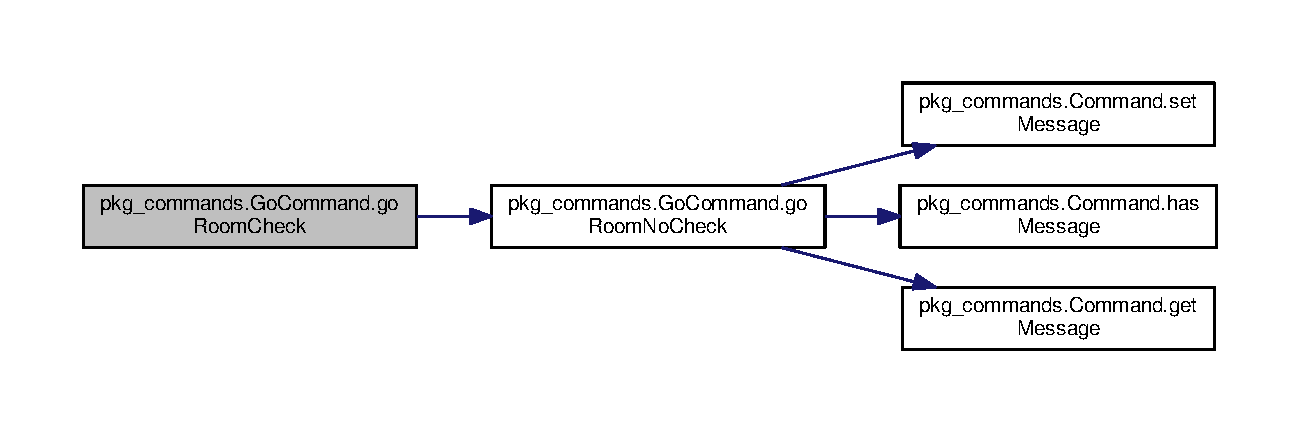
\includegraphics[width=350pt]{classpkg__commands_1_1GoCommand_acbf1aa81fa5b1aef7cafb8b4e3ace3a9_cgraph}
\end{center}
\end{figure}




Here is the caller graph for this function\-:
\nopagebreak
\begin{figure}[H]
\begin{center}
\leavevmode
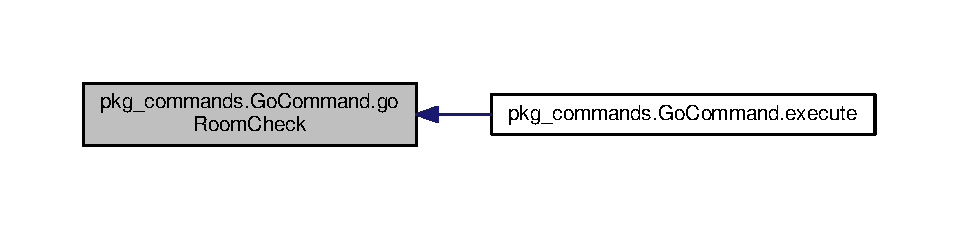
\includegraphics[width=350pt]{classpkg__commands_1_1GoCommand_acbf1aa81fa5b1aef7cafb8b4e3ace3a9_icgraph}
\end{center}
\end{figure}


\hypertarget{classpkg__commands_1_1GoCommand_a210afbc5f3ef34d3ad5759d853c8f8c2}{\index{pkg\-\_\-commands\-::\-Go\-Command@{pkg\-\_\-commands\-::\-Go\-Command}!go\-Room\-No\-Check@{go\-Room\-No\-Check}}
\index{go\-Room\-No\-Check@{go\-Room\-No\-Check}!pkg_commands::GoCommand@{pkg\-\_\-commands\-::\-Go\-Command}}
\subsubsection[{go\-Room\-No\-Check}]{\setlength{\rightskip}{0pt plus 5cm}void pkg\-\_\-commands.\-Go\-Command.\-go\-Room\-No\-Check (
\begin{DoxyParamCaption}
\item[{{\bf Room}}]{room, }
\item[{{\bf Player}}]{player, }
\item[{boolean}]{back}
\end{DoxyParamCaption}
) throws {\bf pkg\-\_\-exceptions.\-Illegal\-Argument\-Exception}\hspace{0.3cm}{\ttfamily [protected]}}}\label{classpkg__commands_1_1GoCommand_a210afbc5f3ef34d3ad5759d853c8f8c2}
Go to the Room without checking. 
\begin{DoxyParams}{Parameters}
{\em room} & Room where the user want to go \\
\hline
{\em player} & The player that called this command \\
\hline
{\em back} & true if it is called via the 'back' command \\
\hline
\end{DoxyParams}

\begin{DoxyExceptions}{Exceptions}
{\em Illegal\-Argument\-Exception} & When the user tries to go to null \\
\hline
\end{DoxyExceptions}


Definition at line \hyperlink{GoCommand_8java_source_l00071}{71} of file \hyperlink{GoCommand_8java_source}{Go\-Command.\-java}.



References \hyperlink{Command_8java_source_l00097}{pkg\-\_\-commands.\-Command.\-get\-Message()}, \hyperlink{Command_8java_source_l00105}{pkg\-\_\-commands.\-Command.\-has\-Message()}, and \hyperlink{Command_8java_source_l00089}{pkg\-\_\-commands.\-Command.\-set\-Message()}.



Referenced by \hyperlink{GoCommand_8java_source_l00032}{pkg\-\_\-commands.\-Go\-Command.\-execute()}, and \hyperlink{GoCommand_8java_source_l00056}{pkg\-\_\-commands.\-Go\-Command.\-go\-Room\-Check()}.


\begin{DoxyCode}
00071                                                                                                            
                   \{
00072         \textcolor{keywordflow}{if}(room != null) \{
00073             \textcolor{keywordflow}{if}(!back)
00074                 player.pushForward();
00075             \textcolor{keywordflow}{else}
00076                 player.popPreviousRooms();
00077             player.goRoom(room);
00078             \hyperlink{classpkg__commands_1_1Command_ae210ff216fe908b111ba1c988a963d13}{setMessage}(((\hyperlink{classpkg__commands_1_1Command_ae46bb048d0fa705a5037a5204b530da2}{hasMessage}()) ? \hyperlink{classpkg__commands_1_1Command_ac2a42e2bab264821892daefaf9a18b6c}{getMessage}() + \textcolor{stringliteral}{"\(\backslash\)n"} : \textcolor{stringliteral}{""}) + room.
      getLongDescription());
00079         \} \textcolor{keywordflow}{else}
00080             \textcolor{keywordflow}{throw} \textcolor{keyword}{new} \hyperlink{classpkg__exceptions_1_1IllegalArgumentException}{pkg\_exceptions.IllegalArgumentException}(\textcolor{stringliteral}{"This
       is a wall, not a door!"});
00081     \}
\end{DoxyCode}


Here is the call graph for this function\-:
\nopagebreak
\begin{figure}[H]
\begin{center}
\leavevmode
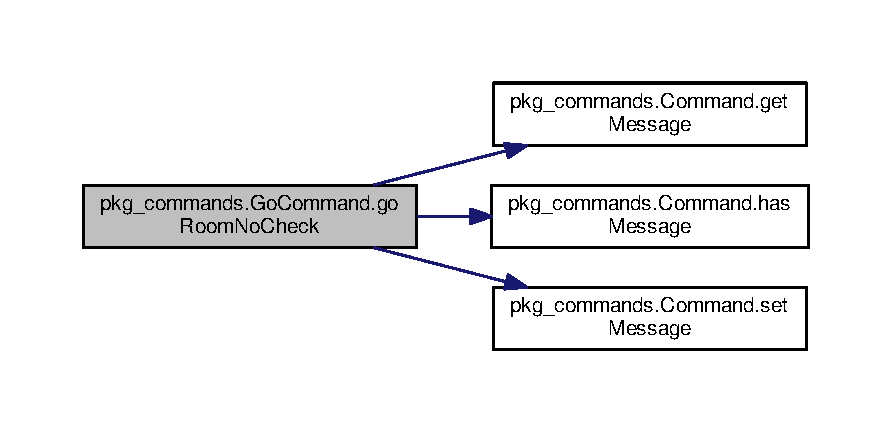
\includegraphics[width=350pt]{classpkg__commands_1_1GoCommand_a210afbc5f3ef34d3ad5759d853c8f8c2_cgraph}
\end{center}
\end{figure}




Here is the caller graph for this function\-:
\nopagebreak
\begin{figure}[H]
\begin{center}
\leavevmode
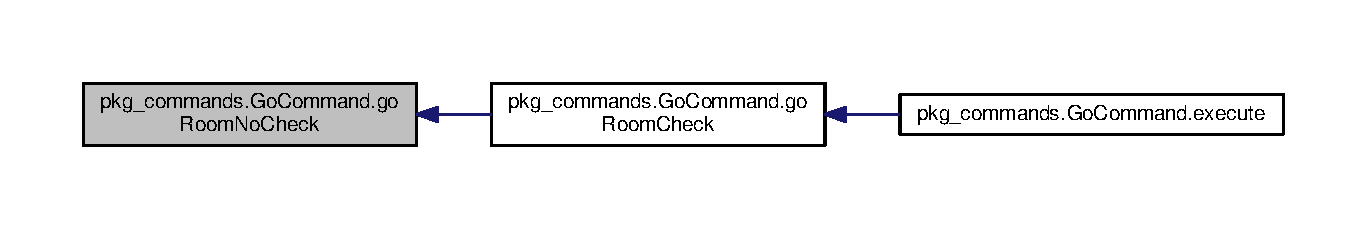
\includegraphics[width=350pt]{classpkg__commands_1_1GoCommand_a210afbc5f3ef34d3ad5759d853c8f8c2_icgraph}
\end{center}
\end{figure}




The documentation for this class was generated from the following file\-:\begin{DoxyCompactItemize}
\item 
pkg\-\_\-commands/\hyperlink{GoCommand_8java}{Go\-Command.\-java}\end{DoxyCompactItemize}

\hypertarget{classpkg__commands_1_1HelpCommand}{\section{pkg\-\_\-commands.\-Help\-Command Class Reference}
\label{classpkg__commands_1_1HelpCommand}\index{pkg\-\_\-commands.\-Help\-Command@{pkg\-\_\-commands.\-Help\-Command}}
}


Inheritance diagram for pkg\-\_\-commands.\-Help\-Command\-:
\nopagebreak
\begin{figure}[H]
\begin{center}
\leavevmode
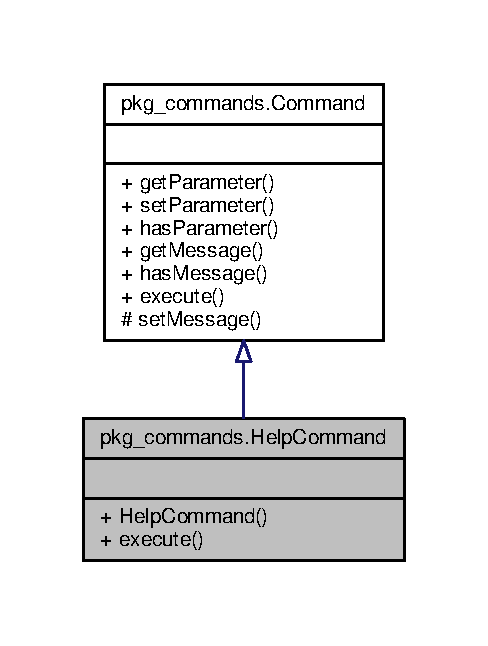
\includegraphics[width=234pt]{classpkg__commands_1_1HelpCommand__inherit__graph}
\end{center}
\end{figure}


Collaboration diagram for pkg\-\_\-commands.\-Help\-Command\-:
\nopagebreak
\begin{figure}[H]
\begin{center}
\leavevmode
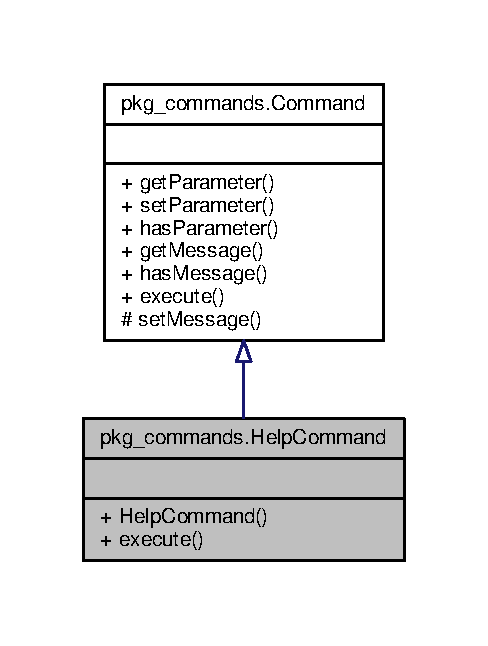
\includegraphics[width=234pt]{classpkg__commands_1_1HelpCommand__coll__graph}
\end{center}
\end{figure}
\subsection*{Public Member Functions}
\begin{DoxyCompactItemize}
\item 
\hyperlink{classpkg__commands_1_1HelpCommand_a5f12eadc1835cd0c7cdb77811b5fb756}{Help\-Command} ()
\item 
boolean \hyperlink{classpkg__commands_1_1HelpCommand_a332d3e57539dfc82f8c539f8b3e24dd6}{execute} (\hyperlink{classpkg__world_1_1Player}{Player} player)
\end{DoxyCompactItemize}
\subsection*{Additional Inherited Members}


\subsection{Detailed Description}
class \hyperlink{classpkg__commands_1_1HelpCommand}{Help\-Command} used to print the help \begin{DoxyAuthor}{Author}
Rémi Nicole 
\end{DoxyAuthor}


Definition at line \hyperlink{HelpCommand_8java_source_l00010}{10} of file \hyperlink{HelpCommand_8java_source}{Help\-Command.\-java}.



\subsection{Constructor \& Destructor Documentation}
\hypertarget{classpkg__commands_1_1HelpCommand_a5f12eadc1835cd0c7cdb77811b5fb756}{\index{pkg\-\_\-commands\-::\-Help\-Command@{pkg\-\_\-commands\-::\-Help\-Command}!Help\-Command@{Help\-Command}}
\index{Help\-Command@{Help\-Command}!pkg_commands::HelpCommand@{pkg\-\_\-commands\-::\-Help\-Command}}
\subsubsection[{Help\-Command}]{\setlength{\rightskip}{0pt plus 5cm}pkg\-\_\-commands.\-Help\-Command.\-Help\-Command (
\begin{DoxyParamCaption}
{}
\end{DoxyParamCaption}
)}}\label{classpkg__commands_1_1HelpCommand_a5f12eadc1835cd0c7cdb77811b5fb756}
Constructor for \hyperlink{classpkg__commands_1_1HelpCommand}{Help\-Command} 

Definition at line \hyperlink{HelpCommand_8java_source_l00023}{23} of file \hyperlink{HelpCommand_8java_source}{Help\-Command.\-java}.


\begin{DoxyCode}
00023                         \{
00024         helpCount = 0;
00025     \}
\end{DoxyCode}


\subsection{Member Function Documentation}
\hypertarget{classpkg__commands_1_1HelpCommand_a332d3e57539dfc82f8c539f8b3e24dd6}{\index{pkg\-\_\-commands\-::\-Help\-Command@{pkg\-\_\-commands\-::\-Help\-Command}!execute@{execute}}
\index{execute@{execute}!pkg_commands::HelpCommand@{pkg\-\_\-commands\-::\-Help\-Command}}
\subsubsection[{execute}]{\setlength{\rightskip}{0pt plus 5cm}boolean pkg\-\_\-commands.\-Help\-Command.\-execute (
\begin{DoxyParamCaption}
\item[{{\bf Player}}]{player}
\end{DoxyParamCaption}
)}}\label{classpkg__commands_1_1HelpCommand_a332d3e57539dfc82f8c539f8b3e24dd6}
Saves user's help in the parameter field. It really shows help if the user asked for more than once the help. 
\begin{DoxyParams}{Parameters}
{\em player} & The player that called this command \\
\hline
\end{DoxyParams}
\begin{DoxyReturn}{Returns}
False because it is not the quit command 
\end{DoxyReturn}


Definition at line \hyperlink{HelpCommand_8java_source_l00033}{33} of file \hyperlink{HelpCommand_8java_source}{Help\-Command.\-java}.



References \hyperlink{Command_8java_source_l00097}{pkg\-\_\-commands.\-Command.\-get\-Message()}, \hyperlink{Command_8java_source_l00089}{pkg\-\_\-commands.\-Command.\-set\-Message()}, and \hyperlink{Parser_8java_source_l00059}{pkg\-\_\-parsing.\-Parser.\-show\-Commands()}.


\begin{DoxyCode}
00033                                           \{
00034         \hyperlink{classpkg__commands_1_1Command_ae210ff216fe908b111ba1c988a963d13}{setMessage}(\textcolor{stringliteral}{""});
00035         \textcolor{keywordflow}{if}(helpCount == 0) \{
00036             \hyperlink{classpkg__commands_1_1Command_ae210ff216fe908b111ba1c988a963d13}{setMessage}(\textcolor{stringliteral}{"Help ? Who needs help ? Only the weak ones."});
00037             ++helpCount;
00038         \} \textcolor{keywordflow}{else} \{
00039             \textcolor{keywordflow}{if}(helpCount == 1)\{
00040                 \hyperlink{classpkg__commands_1_1Command_ae210ff216fe908b111ba1c988a963d13}{setMessage}(\textcolor{stringliteral}{"All right, all right! If you insist...\(\backslash\)n"});
00041                 ++helpCount;
00042             \}
00043             \hyperlink{classpkg__commands_1_1Command_ae210ff216fe908b111ba1c988a963d13}{setMessage}(\hyperlink{classpkg__commands_1_1Command_ac2a42e2bab264821892daefaf9a18b6c}{getMessage}() + \textcolor{stringliteral}{"What you can do is: "} + Parser.showCommands() + \textcolor{stringliteral}{
      "\(\backslash\)n"}
00044                     + \textcolor{stringliteral}{"That will be all."});
00045         \}
00046         \textcolor{keywordflow}{return} \textcolor{keyword}{false};
00047     \}
\end{DoxyCode}


Here is the call graph for this function\-:
\nopagebreak
\begin{figure}[H]
\begin{center}
\leavevmode
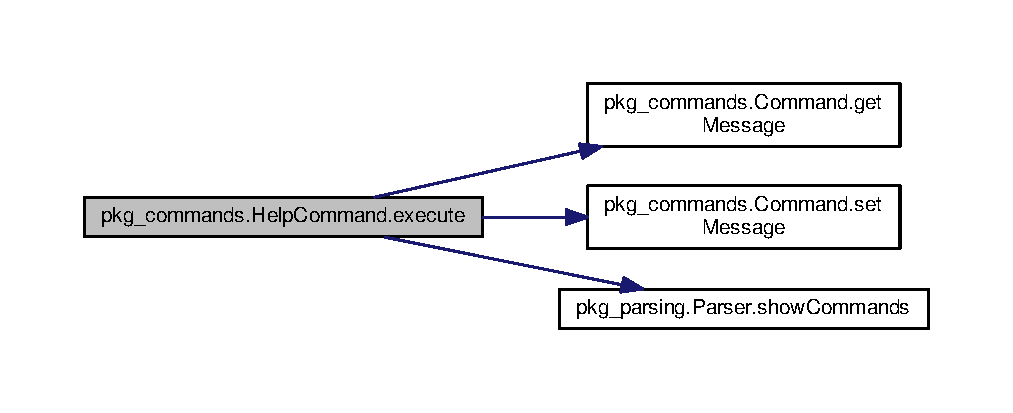
\includegraphics[width=350pt]{classpkg__commands_1_1HelpCommand_a332d3e57539dfc82f8c539f8b3e24dd6_cgraph}
\end{center}
\end{figure}




The documentation for this class was generated from the following file\-:\begin{DoxyCompactItemize}
\item 
pkg\-\_\-commands/\hyperlink{HelpCommand_8java}{Help\-Command.\-java}\end{DoxyCompactItemize}

\hypertarget{classpkg__exceptions_1_1IllegalArgumentException}{\section{pkg\-\_\-exceptions.\-Illegal\-Argument\-Exception Class Reference}
\label{classpkg__exceptions_1_1IllegalArgumentException}\index{pkg\-\_\-exceptions.\-Illegal\-Argument\-Exception@{pkg\-\_\-exceptions.\-Illegal\-Argument\-Exception}}
}


class \hyperlink{classpkg__exceptions_1_1IllegalArgumentException}{Illegal\-Argument\-Exception} used to tell that a command parameter is invalid.  




Inheritance diagram for pkg\-\_\-exceptions.\-Illegal\-Argument\-Exception\-:\nopagebreak
\begin{figure}[H]
\begin{center}
\leavevmode
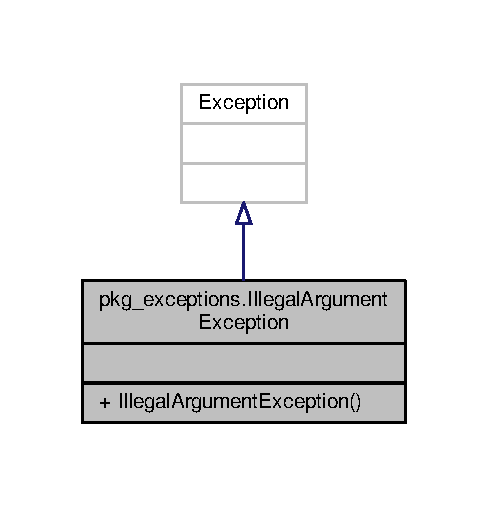
\includegraphics[width=234pt]{classpkg__exceptions_1_1IllegalArgumentException__inherit__graph}
\end{center}
\end{figure}


Collaboration diagram for pkg\-\_\-exceptions.\-Illegal\-Argument\-Exception\-:\nopagebreak
\begin{figure}[H]
\begin{center}
\leavevmode
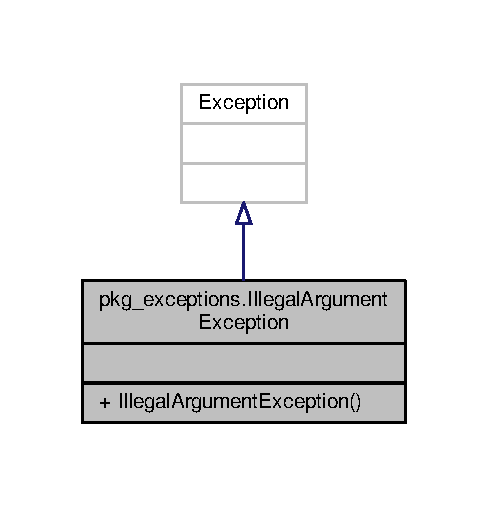
\includegraphics[width=234pt]{classpkg__exceptions_1_1IllegalArgumentException__coll__graph}
\end{center}
\end{figure}
\subsection*{Public Member Functions}
\begin{DoxyCompactItemize}
\item 
\hyperlink{classpkg__exceptions_1_1IllegalArgumentException_a1f9824d1b85743770fd7bd36535ab501}{Illegal\-Argument\-Exception} (String message)
\begin{DoxyCompactList}\small\item\em Constructor for \hyperlink{classpkg__exceptions_1_1IllegalArgumentException}{Illegal\-Argument\-Exception}. \end{DoxyCompactList}\end{DoxyCompactItemize}


\subsection{Detailed Description}
class \hyperlink{classpkg__exceptions_1_1IllegalArgumentException}{Illegal\-Argument\-Exception} used to tell that a command parameter is invalid. 

\begin{DoxyAuthor}{Author}
Rémi Nicole 
\end{DoxyAuthor}


Definition at line \hyperlink{IllegalArgumentException_8java_source_l00007}{7} of file \hyperlink{IllegalArgumentException_8java_source}{Illegal\-Argument\-Exception.\-java}.



\subsection{Constructor \& Destructor Documentation}
\hypertarget{classpkg__exceptions_1_1IllegalArgumentException_a1f9824d1b85743770fd7bd36535ab501}{\index{pkg\-\_\-exceptions\-::\-Illegal\-Argument\-Exception@{pkg\-\_\-exceptions\-::\-Illegal\-Argument\-Exception}!Illegal\-Argument\-Exception@{Illegal\-Argument\-Exception}}
\index{Illegal\-Argument\-Exception@{Illegal\-Argument\-Exception}!pkg_exceptions::IllegalArgumentException@{pkg\-\_\-exceptions\-::\-Illegal\-Argument\-Exception}}
\subsubsection[{Illegal\-Argument\-Exception}]{\setlength{\rightskip}{0pt plus 5cm}pkg\-\_\-exceptions.\-Illegal\-Argument\-Exception.\-Illegal\-Argument\-Exception (
\begin{DoxyParamCaption}
\item[{String}]{message}
\end{DoxyParamCaption}
)}}\label{classpkg__exceptions_1_1IllegalArgumentException_a1f9824d1b85743770fd7bd36535ab501}


Constructor for \hyperlink{classpkg__exceptions_1_1IllegalArgumentException}{Illegal\-Argument\-Exception}. 


\begin{DoxyParams}{Parameters}
{\em message} & Message to display in case of that error \\
\hline
\end{DoxyParams}


Definition at line \hyperlink{IllegalArgumentException_8java_source_l00013}{13} of file \hyperlink{IllegalArgumentException_8java_source}{Illegal\-Argument\-Exception.\-java}.


\begin{DoxyCode}
00013                                                    \{
00014         super(message);
00015     \}
\end{DoxyCode}


The documentation for this class was generated from the following file\-:\begin{DoxyCompactItemize}
\item 
pkg\-\_\-exceptions/\hyperlink{IllegalArgumentException_8java}{Illegal\-Argument\-Exception.\-java}\end{DoxyCompactItemize}

\hypertarget{classpkg__commands_1_1InventoryCommand}{\section{pkg\-\_\-commands.\-Inventory\-Command Class Reference}
\label{classpkg__commands_1_1InventoryCommand}\index{pkg\-\_\-commands.\-Inventory\-Command@{pkg\-\_\-commands.\-Inventory\-Command}}
}


Inheritance diagram for pkg\-\_\-commands.\-Inventory\-Command\-:
\nopagebreak
\begin{figure}[H]
\begin{center}
\leavevmode
\includegraphics[width=254pt]{classpkg__commands_1_1InventoryCommand__inherit__graph}
\end{center}
\end{figure}


Collaboration diagram for pkg\-\_\-commands.\-Inventory\-Command\-:
\nopagebreak
\begin{figure}[H]
\begin{center}
\leavevmode
\includegraphics[width=254pt]{classpkg__commands_1_1InventoryCommand__coll__graph}
\end{center}
\end{figure}
\subsection*{Public Member Functions}
\begin{DoxyCompactItemize}
\item 
\hyperlink{classpkg__commands_1_1InventoryCommand_a4ca959fe6979e5ca2a79a0596803533d}{Inventory\-Command} ()
\item 
boolean \hyperlink{classpkg__commands_1_1InventoryCommand_a16ce9e3db461ecb7c4a50d2bdef65022}{execute} (\hyperlink{classpkg__world_1_1Player}{Player} player)
\end{DoxyCompactItemize}
\subsection*{Additional Inherited Members}


\subsection{Detailed Description}
class \hyperlink{classpkg__commands_1_1InventoryCommand}{Inventory\-Command} used to print the player's inventory \begin{DoxyAuthor}{Author}
Rémi Nicole 
\end{DoxyAuthor}


Definition at line \hyperlink{InventoryCommand_8java_source_l00009}{9} of file \hyperlink{InventoryCommand_8java_source}{Inventory\-Command.\-java}.



\subsection{Constructor \& Destructor Documentation}
\hypertarget{classpkg__commands_1_1InventoryCommand_a4ca959fe6979e5ca2a79a0596803533d}{\index{pkg\-\_\-commands\-::\-Inventory\-Command@{pkg\-\_\-commands\-::\-Inventory\-Command}!Inventory\-Command@{Inventory\-Command}}
\index{Inventory\-Command@{Inventory\-Command}!pkg_commands::InventoryCommand@{pkg\-\_\-commands\-::\-Inventory\-Command}}
\subsubsection[{Inventory\-Command}]{\setlength{\rightskip}{0pt plus 5cm}pkg\-\_\-commands.\-Inventory\-Command.\-Inventory\-Command (
\begin{DoxyParamCaption}
{}
\end{DoxyParamCaption}
)}}\label{classpkg__commands_1_1InventoryCommand_a4ca959fe6979e5ca2a79a0596803533d}
Constructor for \hyperlink{classpkg__commands_1_1InventoryCommand}{Inventory\-Command} 

Definition at line \hyperlink{InventoryCommand_8java_source_l00014}{14} of file \hyperlink{InventoryCommand_8java_source}{Inventory\-Command.\-java}.


\begin{DoxyCode}
00014                              \{
00015 
00016     \}
\end{DoxyCode}


\subsection{Member Function Documentation}
\hypertarget{classpkg__commands_1_1InventoryCommand_a16ce9e3db461ecb7c4a50d2bdef65022}{\index{pkg\-\_\-commands\-::\-Inventory\-Command@{pkg\-\_\-commands\-::\-Inventory\-Command}!execute@{execute}}
\index{execute@{execute}!pkg_commands::InventoryCommand@{pkg\-\_\-commands\-::\-Inventory\-Command}}
\subsubsection[{execute}]{\setlength{\rightskip}{0pt plus 5cm}boolean pkg\-\_\-commands.\-Inventory\-Command.\-execute (
\begin{DoxyParamCaption}
\item[{{\bf Player}}]{player}
\end{DoxyParamCaption}
)}}\label{classpkg__commands_1_1InventoryCommand_a16ce9e3db461ecb7c4a50d2bdef65022}
Save the inventory into the message field. 
\begin{DoxyParams}{Parameters}
{\em player} & The player that called this command \\
\hline
\end{DoxyParams}
\begin{DoxyReturn}{Returns}
False because it is not the quit command 
\end{DoxyReturn}


Definition at line \hyperlink{InventoryCommand_8java_source_l00023}{23} of file \hyperlink{InventoryCommand_8java_source}{Inventory\-Command.\-java}.



References \hyperlink{Player_8java_source_l00219}{pkg\-\_\-world.\-Player.\-get\-Inventory()}, and \hyperlink{Command_8java_source_l00058}{pkg\-\_\-commands.\-Command.\-set\-Message()}.


\begin{DoxyCode}
00023                                           \{
00024         \hyperlink{classpkg__commands_1_1Command_ae210ff216fe908b111ba1c988a963d13}{setMessage}(player.getInventory());
00025         \textcolor{keywordflow}{return} \textcolor{keyword}{false};
00026     \}
\end{DoxyCode}


Here is the call graph for this function\-:
\nopagebreak
\begin{figure}[H]
\begin{center}
\leavevmode
\includegraphics[width=350pt]{classpkg__commands_1_1InventoryCommand_a16ce9e3db461ecb7c4a50d2bdef65022_cgraph}
\end{center}
\end{figure}




The documentation for this class was generated from the following file\-:\begin{DoxyCompactItemize}
\item 
pkg\-\_\-commands/\hyperlink{InventoryCommand_8java}{Inventory\-Command.\-java}\end{DoxyCompactItemize}

\hypertarget{classpkg__world_1_1Item}{\section{pkg\-\_\-world.\-Item Class Reference}
\label{classpkg__world_1_1Item}\index{pkg\-\_\-world.\-Item@{pkg\-\_\-world.\-Item}}
}


Collaboration diagram for pkg\-\_\-world.\-Item\-:
\nopagebreak
\begin{figure}[H]
\begin{center}
\leavevmode
\includegraphics[width=174pt]{classpkg__world_1_1Item__coll__graph}
\end{center}
\end{figure}
\subsection*{Public Member Functions}
\begin{DoxyCompactItemize}
\item 
\hyperlink{classpkg__world_1_1Item_a57474f01fd9f40be8d01edc1ad79171c}{Item} (String name, int weight, String description)
\item 
String \hyperlink{classpkg__world_1_1Item_a2ac9495ef1a08f01df7f66a46ca895c2}{get\-Name} ()
\item 
int \hyperlink{classpkg__world_1_1Item_a4e4d16b3d657683d482e4e131f8d0571}{get\-Weight} ()
\item 
String \hyperlink{classpkg__world_1_1Item_a2fb9a737f363fe6c0a50280c8630fcd0}{get\-Description} ()
\end{DoxyCompactItemize}


\subsection{Detailed Description}
Class used to handle an item contained in a \hyperlink{classpkg__world_1_1Room}{Room}. \begin{DoxyAuthor}{Author}
Rémi Nicole 
\end{DoxyAuthor}


Definition at line \hyperlink{Item_8java_source_l00007}{7} of file \hyperlink{Item_8java_source}{Item.\-java}.



\subsection{Constructor \& Destructor Documentation}
\hypertarget{classpkg__world_1_1Item_a57474f01fd9f40be8d01edc1ad79171c}{\index{pkg\-\_\-world\-::\-Item@{pkg\-\_\-world\-::\-Item}!Item@{Item}}
\index{Item@{Item}!pkg_world::Item@{pkg\-\_\-world\-::\-Item}}
\subsubsection[{Item}]{\setlength{\rightskip}{0pt plus 5cm}pkg\-\_\-world.\-Item.\-Item (
\begin{DoxyParamCaption}
\item[{String}]{name, }
\item[{int}]{weight, }
\item[{String}]{description}
\end{DoxyParamCaption}
)}}\label{classpkg__world_1_1Item_a57474f01fd9f40be8d01edc1ad79171c}
\hyperlink{classpkg__world_1_1Item}{Item} class constructor. 
\begin{DoxyParams}{Parameters}
{\em name} & Name of the item \\
\hline
{\em weight} & Weight of the item \\
\hline
{\em description} & Description of the item \\
\hline
\end{DoxyParams}


Definition at line \hyperlink{Item_8java_source_l00030}{30} of file \hyperlink{Item_8java_source}{Item.\-java}.


\begin{DoxyCode}
00030                                                              \{
00031         this.name = name;
00032         this.weight = weight;
00033         this.description = description;
00034     \}
\end{DoxyCode}


\subsection{Member Function Documentation}
\hypertarget{classpkg__world_1_1Item_a2fb9a737f363fe6c0a50280c8630fcd0}{\index{pkg\-\_\-world\-::\-Item@{pkg\-\_\-world\-::\-Item}!get\-Description@{get\-Description}}
\index{get\-Description@{get\-Description}!pkg_world::Item@{pkg\-\_\-world\-::\-Item}}
\subsubsection[{get\-Description}]{\setlength{\rightskip}{0pt plus 5cm}String pkg\-\_\-world.\-Item.\-get\-Description (
\begin{DoxyParamCaption}
{}
\end{DoxyParamCaption}
)}}\label{classpkg__world_1_1Item_a2fb9a737f363fe6c0a50280c8630fcd0}
description field getter. \begin{DoxyReturn}{Returns}
The description of the item 
\end{DoxyReturn}


Definition at line \hyperlink{Item_8java_source_l00056}{56} of file \hyperlink{Item_8java_source}{Item.\-java}.


\begin{DoxyCode}
00056                                    \{
00057         \textcolor{keywordflow}{return} description;
00058     \}
\end{DoxyCode}
\hypertarget{classpkg__world_1_1Item_a2ac9495ef1a08f01df7f66a46ca895c2}{\index{pkg\-\_\-world\-::\-Item@{pkg\-\_\-world\-::\-Item}!get\-Name@{get\-Name}}
\index{get\-Name@{get\-Name}!pkg_world::Item@{pkg\-\_\-world\-::\-Item}}
\subsubsection[{get\-Name}]{\setlength{\rightskip}{0pt plus 5cm}String pkg\-\_\-world.\-Item.\-get\-Name (
\begin{DoxyParamCaption}
{}
\end{DoxyParamCaption}
)}}\label{classpkg__world_1_1Item_a2ac9495ef1a08f01df7f66a46ca895c2}
name field getter. \begin{DoxyReturn}{Returns}
The name of the item 
\end{DoxyReturn}


Definition at line \hyperlink{Item_8java_source_l00040}{40} of file \hyperlink{Item_8java_source}{Item.\-java}.



Referenced by \hyperlink{Player_8java_source_l00192}{pkg\-\_\-world.\-Player.\-take\-Object()}.


\begin{DoxyCode}
00040                             \{
00041         \textcolor{keywordflow}{return} name;
00042     \}
\end{DoxyCode}


Here is the caller graph for this function\-:
\nopagebreak
\begin{figure}[H]
\begin{center}
\leavevmode
\includegraphics[width=350pt]{classpkg__world_1_1Item_a2ac9495ef1a08f01df7f66a46ca895c2_icgraph}
\end{center}
\end{figure}


\hypertarget{classpkg__world_1_1Item_a4e4d16b3d657683d482e4e131f8d0571}{\index{pkg\-\_\-world\-::\-Item@{pkg\-\_\-world\-::\-Item}!get\-Weight@{get\-Weight}}
\index{get\-Weight@{get\-Weight}!pkg_world::Item@{pkg\-\_\-world\-::\-Item}}
\subsubsection[{get\-Weight}]{\setlength{\rightskip}{0pt plus 5cm}int pkg\-\_\-world.\-Item.\-get\-Weight (
\begin{DoxyParamCaption}
{}
\end{DoxyParamCaption}
)}}\label{classpkg__world_1_1Item_a4e4d16b3d657683d482e4e131f8d0571}
weight field getter. \begin{DoxyReturn}{Returns}
The weight of the item 
\end{DoxyReturn}


Definition at line \hyperlink{Item_8java_source_l00048}{48} of file \hyperlink{Item_8java_source}{Item.\-java}.


\begin{DoxyCode}
00048                            \{
00049         \textcolor{keywordflow}{return} weight;
00050     \}
\end{DoxyCode}


The documentation for this class was generated from the following file\-:\begin{DoxyCompactItemize}
\item 
pkg\-\_\-world/\hyperlink{Item_8java}{Item.\-java}\end{DoxyCompactItemize}

\hypertarget{classpkg__world_1_1ItemList}{\section{pkg\-\_\-world.\-Item\-List Class Reference}
\label{classpkg__world_1_1ItemList}\index{pkg\-\_\-world.\-Item\-List@{pkg\-\_\-world.\-Item\-List}}
}


Inheritance diagram for pkg\-\_\-world.\-Item\-List\-:
\nopagebreak
\begin{figure}[H]
\begin{center}
\leavevmode
\includegraphics[width=180pt]{classpkg__world_1_1ItemList__inherit__graph}
\end{center}
\end{figure}


Collaboration diagram for pkg\-\_\-world.\-Item\-List\-:
\nopagebreak
\begin{figure}[H]
\begin{center}
\leavevmode
\includegraphics[width=180pt]{classpkg__world_1_1ItemList__coll__graph}
\end{center}
\end{figure}
\subsection*{Public Member Functions}
\begin{DoxyCompactItemize}
\item 
void \hyperlink{classpkg__world_1_1ItemList_a0428375741d0442813d88131a5962a10}{transfer} (String item, Hash\-Map$<$ String, \hyperlink{classpkg__world_1_1Item}{Item} $>$ item\-Map)
\end{DoxyCompactItemize}


\subsection{Detailed Description}
class \hyperlink{classpkg__world_1_1ItemList}{Item\-List} used to handle a list of \hyperlink{classpkg__world_1_1Item}{Item} (inventory). \begin{DoxyAuthor}{Author}
Rémi N\-I\-C\-O\-L\-E 
\end{DoxyAuthor}


Definition at line \hyperlink{ItemList_8java_source_l00009}{9} of file \hyperlink{ItemList_8java_source}{Item\-List.\-java}.



\subsection{Member Function Documentation}
\hypertarget{classpkg__world_1_1ItemList_a0428375741d0442813d88131a5962a10}{\index{pkg\-\_\-world\-::\-Item\-List@{pkg\-\_\-world\-::\-Item\-List}!transfer@{transfer}}
\index{transfer@{transfer}!pkg_world::ItemList@{pkg\-\_\-world\-::\-Item\-List}}
\subsubsection[{transfer}]{\setlength{\rightskip}{0pt plus 5cm}void pkg\-\_\-world.\-Item\-List.\-transfer (
\begin{DoxyParamCaption}
\item[{String}]{item, }
\item[{Hash\-Map$<$ String, {\bf Item} $>$}]{item\-Map}
\end{DoxyParamCaption}
)}}\label{classpkg__world_1_1ItemList_a0428375741d0442813d88131a5962a10}
Transfer a given item to another \hyperlink{classpkg__world_1_1ItemList}{Item\-List} or Hash\-Map 
\begin{DoxyParams}{Parameters}
{\em item} & \hyperlink{classpkg__world_1_1Item}{Item} to be transferred \\
\hline
{\em item\-Map} & Map of items in which the item is transferred \\
\hline
\end{DoxyParams}


Definition at line \hyperlink{ItemList_8java_source_l00016}{16} of file \hyperlink{ItemList_8java_source}{Item\-List.\-java}.


\begin{DoxyCode}
00016                                                                      \{
00017         itemMap.put(item, this.remove(item));
00018     \}
\end{DoxyCode}


The documentation for this class was generated from the following file\-:\begin{DoxyCompactItemize}
\item 
pkg\-\_\-world/\hyperlink{ItemList_8java}{Item\-List.\-java}\end{DoxyCompactItemize}

\hypertarget{classpkg__commands_1_1LookCommand}{\section{pkg\-\_\-commands.\-Look\-Command Class Reference}
\label{classpkg__commands_1_1LookCommand}\index{pkg\-\_\-commands.\-Look\-Command@{pkg\-\_\-commands.\-Look\-Command}}
}


class \hyperlink{classpkg__commands_1_1LookCommand}{Look\-Command} used to show information about the current Room or a given Item  




Inheritance diagram for pkg\-\_\-commands.\-Look\-Command\-:\nopagebreak
\begin{figure}[H]
\begin{center}
\leavevmode
\includegraphics[width=234pt]{classpkg__commands_1_1LookCommand__inherit__graph}
\end{center}
\end{figure}


Collaboration diagram for pkg\-\_\-commands.\-Look\-Command\-:\nopagebreak
\begin{figure}[H]
\begin{center}
\leavevmode
\includegraphics[width=234pt]{classpkg__commands_1_1LookCommand__coll__graph}
\end{center}
\end{figure}
\subsection*{Public Member Functions}
\begin{DoxyCompactItemize}
\item 
\hyperlink{classpkg__commands_1_1LookCommand_ab689f51a18ea2d40ab995099e076112c}{Look\-Command} ()
\begin{DoxyCompactList}\small\item\em Constructor for \hyperlink{classpkg__commands_1_1LookCommand}{Look\-Command}. \end{DoxyCompactList}\item 
boolean \hyperlink{classpkg__commands_1_1LookCommand_af336146fae1e14bf434d85a5acbcdcd7}{execute} (\hyperlink{classpkg__world_1_1Player}{Player} player)  throws Illegal\-Argument\-Exception 
\begin{DoxyCompactList}\small\item\em Saves the information about the current Room or a given Item in the message field. \end{DoxyCompactList}\end{DoxyCompactItemize}
\subsection*{Private Member Functions}
\begin{DoxyCompactItemize}
\item 
String \hyperlink{classpkg__commands_1_1LookCommand_a17808882dffb0a9edce192235c029ddf}{show\-Item} (\hyperlink{classpkg__world_1_1Item}{Item} item)
\begin{DoxyCompactList}\small\item\em Return a given Item's description. \end{DoxyCompactList}\end{DoxyCompactItemize}
\subsection*{Additional Inherited Members}


\subsection{Detailed Description}
class \hyperlink{classpkg__commands_1_1LookCommand}{Look\-Command} used to show information about the current Room or a given Item 

\begin{DoxyAuthor}{Author}
Rémi Nicole 
\end{DoxyAuthor}


Definition at line \hyperlink{LookCommand_8java_source_l00011}{11} of file \hyperlink{LookCommand_8java_source}{Look\-Command.\-java}.



\subsection{Constructor \& Destructor Documentation}
\hypertarget{classpkg__commands_1_1LookCommand_ab689f51a18ea2d40ab995099e076112c}{\index{pkg\-\_\-commands\-::\-Look\-Command@{pkg\-\_\-commands\-::\-Look\-Command}!Look\-Command@{Look\-Command}}
\index{Look\-Command@{Look\-Command}!pkg_commands::LookCommand@{pkg\-\_\-commands\-::\-Look\-Command}}
\subsubsection[{Look\-Command}]{\setlength{\rightskip}{0pt plus 5cm}pkg\-\_\-commands.\-Look\-Command.\-Look\-Command (
\begin{DoxyParamCaption}
{}
\end{DoxyParamCaption}
)}}\label{classpkg__commands_1_1LookCommand_ab689f51a18ea2d40ab995099e076112c}


Constructor for \hyperlink{classpkg__commands_1_1LookCommand}{Look\-Command}. 



Definition at line \hyperlink{LookCommand_8java_source_l00016}{16} of file \hyperlink{LookCommand_8java_source}{Look\-Command.\-java}.


\begin{DoxyCode}
00016                         \{
00017 
00018     \}
\end{DoxyCode}


\subsection{Member Function Documentation}
\hypertarget{classpkg__commands_1_1LookCommand_af336146fae1e14bf434d85a5acbcdcd7}{\index{pkg\-\_\-commands\-::\-Look\-Command@{pkg\-\_\-commands\-::\-Look\-Command}!execute@{execute}}
\index{execute@{execute}!pkg_commands::LookCommand@{pkg\-\_\-commands\-::\-Look\-Command}}
\subsubsection[{execute}]{\setlength{\rightskip}{0pt plus 5cm}boolean pkg\-\_\-commands.\-Look\-Command.\-execute (
\begin{DoxyParamCaption}
\item[{{\bf Player}}]{player}
\end{DoxyParamCaption}
) throws {\bf Illegal\-Argument\-Exception}}}\label{classpkg__commands_1_1LookCommand_af336146fae1e14bf434d85a5acbcdcd7}


Saves the information about the current Room or a given Item in the message field. 


\begin{DoxyParams}{Parameters}
{\em player} & The player that called this command \\
\hline
\end{DoxyParams}

\begin{DoxyExceptions}{Exceptions}
{\em Illegal\-Argument\-Exception} & When the user typed a name other than any of the items in the Player's or the Room's inventory \\
\hline
\end{DoxyExceptions}
\begin{DoxyReturn}{Returns}
False because it is not the quit command 
\end{DoxyReturn}


Definition at line \hyperlink{LookCommand_8java_source_l00026}{26} of file \hyperlink{LookCommand_8java_source}{Look\-Command.\-java}.



References \hyperlink{Command_8java_source_l00034}{pkg\-\_\-commands.\-Command.\-get\-Parameter()}, \hyperlink{Command_8java_source_l00050}{pkg\-\_\-commands.\-Command.\-has\-Parameter()}, \hyperlink{Command_8java_source_l00058}{pkg\-\_\-commands.\-Command.\-set\-Message()}, and \hyperlink{LookCommand_8java_source_l00048}{pkg\-\_\-commands.\-Look\-Command.\-show\-Item()}.


\begin{DoxyCode}
00026                                                                           \{
00027         \textcolor{keywordflow}{if}(\hyperlink{classpkg__commands_1_1Command_a02af95ab3f1898a66259ab7c177b6998}{hasParameter}()) \{
00028             \textcolor{keywordflow}{if}(player.getCurrentRoom().hasItem(\hyperlink{classpkg__commands_1_1Command_a41c92d445be73ea9d62320c65efb8434}{getParameter}())) \{
00029                 \hyperlink{classpkg__commands_1_1Command_ae210ff216fe908b111ba1c988a963d13}{setMessage}(
00030                         \hyperlink{classpkg__commands_1_1LookCommand_a17808882dffb0a9edce192235c029ddf}{showItem}(player.getCurrentRoom().getItem(
      \hyperlink{classpkg__commands_1_1Command_a41c92d445be73ea9d62320c65efb8434}{getParameter}()))
00031                         );
00032             \} \textcolor{keywordflow}{else} \textcolor{keywordflow}{if} (player.hasItem(\hyperlink{classpkg__commands_1_1Command_a41c92d445be73ea9d62320c65efb8434}{getParameter}()) ) \{
00033                 \hyperlink{classpkg__commands_1_1Command_ae210ff216fe908b111ba1c988a963d13}{setMessage}(
00034                         \hyperlink{classpkg__commands_1_1LookCommand_a17808882dffb0a9edce192235c029ddf}{showItem}(player.getItem(\hyperlink{classpkg__commands_1_1Command_a41c92d445be73ea9d62320c65efb8434}{getParameter}()))
00035                         );
00036             \} \textcolor{keywordflow}{else}
00037                 \textcolor{keywordflow}{throw} \textcolor{keyword}{new} IllegalArgumentException( \textcolor{stringliteral}{"I'm not sure you want to look at that."});
00038         \} \textcolor{keywordflow}{else}
00039             \hyperlink{classpkg__commands_1_1Command_ae210ff216fe908b111ba1c988a963d13}{setMessage}(player.getCurrentRoom().getLongDescription());
00040         \textcolor{keywordflow}{return} \textcolor{keyword}{false};
00041     \}
\end{DoxyCode}


Here is the call graph for this function\-:\nopagebreak
\begin{figure}[H]
\begin{center}
\leavevmode
\includegraphics[width=350pt]{classpkg__commands_1_1LookCommand_af336146fae1e14bf434d85a5acbcdcd7_cgraph}
\end{center}
\end{figure}


\hypertarget{classpkg__commands_1_1LookCommand_a17808882dffb0a9edce192235c029ddf}{\index{pkg\-\_\-commands\-::\-Look\-Command@{pkg\-\_\-commands\-::\-Look\-Command}!show\-Item@{show\-Item}}
\index{show\-Item@{show\-Item}!pkg_commands::LookCommand@{pkg\-\_\-commands\-::\-Look\-Command}}
\subsubsection[{show\-Item}]{\setlength{\rightskip}{0pt plus 5cm}String pkg\-\_\-commands.\-Look\-Command.\-show\-Item (
\begin{DoxyParamCaption}
\item[{{\bf Item}}]{item}
\end{DoxyParamCaption}
)\hspace{0.3cm}{\ttfamily [private]}}}\label{classpkg__commands_1_1LookCommand_a17808882dffb0a9edce192235c029ddf}


Return a given Item's description. 


\begin{DoxyParams}{Parameters}
{\em item} & The item for which we want the description \\
\hline
\end{DoxyParams}
\begin{DoxyReturn}{Returns}
The item's description 
\end{DoxyReturn}


Definition at line \hyperlink{LookCommand_8java_source_l00048}{48} of file \hyperlink{LookCommand_8java_source}{Look\-Command.\-java}.



Referenced by \hyperlink{LookCommand_8java_source_l00026}{pkg\-\_\-commands.\-Look\-Command.\-execute()}.


\begin{DoxyCode}
00048                                        \{
00049         \textcolor{keywordflow}{return} \textcolor{stringliteral}{"This is "} + item.getDescription() + \textcolor{stringliteral}{"."};
00050     \}
\end{DoxyCode}


Here is the caller graph for this function\-:\nopagebreak
\begin{figure}[H]
\begin{center}
\leavevmode
\includegraphics[width=350pt]{classpkg__commands_1_1LookCommand_a17808882dffb0a9edce192235c029ddf_icgraph}
\end{center}
\end{figure}




The documentation for this class was generated from the following file\-:\begin{DoxyCompactItemize}
\item 
pkg\-\_\-commands/\hyperlink{LookCommand_8java}{Look\-Command.\-java}\end{DoxyCompactItemize}

\hypertarget{classpkg__exceptions_1_1NoArgumentException}{\section{pkg\-\_\-exceptions.\-No\-Argument\-Exception Class Reference}
\label{classpkg__exceptions_1_1NoArgumentException}\index{pkg\-\_\-exceptions.\-No\-Argument\-Exception@{pkg\-\_\-exceptions.\-No\-Argument\-Exception}}
}


class \hyperlink{classpkg__exceptions_1_1NoArgumentException}{No\-Argument\-Exception} used to tell that a given command must have a parameter.  




Inheritance diagram for pkg\-\_\-exceptions.\-No\-Argument\-Exception\-:
\nopagebreak
\begin{figure}[H]
\begin{center}
\leavevmode
\includegraphics[width=222pt]{classpkg__exceptions_1_1NoArgumentException__inherit__graph}
\end{center}
\end{figure}


Collaboration diagram for pkg\-\_\-exceptions.\-No\-Argument\-Exception\-:
\nopagebreak
\begin{figure}[H]
\begin{center}
\leavevmode
\includegraphics[width=222pt]{classpkg__exceptions_1_1NoArgumentException__coll__graph}
\end{center}
\end{figure}
\subsection*{Public Member Functions}
\begin{DoxyCompactItemize}
\item 
\hyperlink{classpkg__exceptions_1_1NoArgumentException_a181d2724e9f33f9bd29b1292d4ac9c08}{No\-Argument\-Exception} (String message)
\begin{DoxyCompactList}\small\item\em Constructor for \hyperlink{classpkg__exceptions_1_1NoArgumentException}{No\-Argument\-Exception}. \end{DoxyCompactList}\end{DoxyCompactItemize}


\subsection{Detailed Description}
class \hyperlink{classpkg__exceptions_1_1NoArgumentException}{No\-Argument\-Exception} used to tell that a given command must have a parameter. 

\begin{DoxyAuthor}{Author}
Rémi Nicole 
\end{DoxyAuthor}


Definition at line \hyperlink{NoArgumentException_8java_source_l00011}{11} of file \hyperlink{NoArgumentException_8java_source}{No\-Argument\-Exception.\-java}.



\subsection{Constructor \& Destructor Documentation}
\hypertarget{classpkg__exceptions_1_1NoArgumentException_a181d2724e9f33f9bd29b1292d4ac9c08}{\index{pkg\-\_\-exceptions\-::\-No\-Argument\-Exception@{pkg\-\_\-exceptions\-::\-No\-Argument\-Exception}!No\-Argument\-Exception@{No\-Argument\-Exception}}
\index{No\-Argument\-Exception@{No\-Argument\-Exception}!pkg_exceptions::NoArgumentException@{pkg\-\_\-exceptions\-::\-No\-Argument\-Exception}}
\subsubsection[{No\-Argument\-Exception}]{\setlength{\rightskip}{0pt plus 5cm}pkg\-\_\-exceptions.\-No\-Argument\-Exception.\-No\-Argument\-Exception (
\begin{DoxyParamCaption}
\item[{String}]{message}
\end{DoxyParamCaption}
)}}\label{classpkg__exceptions_1_1NoArgumentException_a181d2724e9f33f9bd29b1292d4ac9c08}


Constructor for \hyperlink{classpkg__exceptions_1_1NoArgumentException}{No\-Argument\-Exception}. 


\begin{DoxyParams}{Parameters}
{\em message} & Message to display in case of that error \\
\hline
\end{DoxyParams}


Definition at line \hyperlink{NoArgumentException_8java_source_l00017}{17} of file \hyperlink{NoArgumentException_8java_source}{No\-Argument\-Exception.\-java}.


\begin{DoxyCode}
00017                                               \{
00018         super(message);
00019     \}
\end{DoxyCode}


The documentation for this class was generated from the following file\-:\begin{DoxyCompactItemize}
\item 
pkg\-\_\-exceptions/\hyperlink{NoArgumentException_8java}{No\-Argument\-Exception.\-java}\end{DoxyCompactItemize}

\hypertarget{classpkg__parsing_1_1Parser}{\section{pkg\-\_\-parsing.\-Parser Class Reference}
\label{classpkg__parsing_1_1Parser}\index{pkg\-\_\-parsing.\-Parser@{pkg\-\_\-parsing.\-Parser}}
}


Collaboration diagram for pkg\-\_\-parsing.\-Parser\-:
\nopagebreak
\begin{figure}[H]
\begin{center}
\leavevmode
\includegraphics[width=184pt]{classpkg__parsing_1_1Parser__coll__graph}
\end{center}
\end{figure}
\subsection*{Static Public Member Functions}
\begin{DoxyCompactItemize}
\item 
static \hyperlink{classpkg__commands_1_1Command}{Command} \hyperlink{classpkg__parsing_1_1Parser_a3baac59980671aeb689ca25fba64e9cc}{get\-Command} (String input\-Line)
\item 
static String \hyperlink{classpkg__parsing_1_1Parser_a31545cdbdb409aaeb727289c0ea7be1b}{show\-Commands} ()
\end{DoxyCompactItemize}


\subsection{Detailed Description}
Class used to parse the commands with or without parameters given by the user. \begin{DoxyAuthor}{Author}
Rémi N\-I\-C\-O\-L\-E 
\end{DoxyAuthor}


Definition at line \hyperlink{Parser_8java_source_l00016}{16} of file \hyperlink{Parser_8java_source}{Parser.\-java}.



\subsection{Member Function Documentation}
\hypertarget{classpkg__parsing_1_1Parser_a3baac59980671aeb689ca25fba64e9cc}{\index{pkg\-\_\-parsing\-::\-Parser@{pkg\-\_\-parsing\-::\-Parser}!get\-Command@{get\-Command}}
\index{get\-Command@{get\-Command}!pkg_parsing::Parser@{pkg\-\_\-parsing\-::\-Parser}}
\subsubsection[{get\-Command}]{\setlength{\rightskip}{0pt plus 5cm}static {\bf Command} pkg\-\_\-parsing.\-Parser.\-get\-Command (
\begin{DoxyParamCaption}
\item[{String}]{input\-Line}
\end{DoxyParamCaption}
)\hspace{0.3cm}{\ttfamily [static]}}}\label{classpkg__parsing_1_1Parser_a3baac59980671aeb689ca25fba64e9cc}
Return the Command corresponding to the given user's input. 
\begin{DoxyParams}{Parameters}
{\em input\-Line} & The user's input \\
\hline
\end{DoxyParams}
\begin{DoxyReturn}{Returns}
The corresponding Command 
\end{DoxyReturn}


Definition at line \hyperlink{Parser_8java_source_l00028}{28} of file \hyperlink{Parser_8java_source}{Parser.\-java}.


\begin{DoxyCode}
00028                                                        \{
00029 
00030         String word1, word2, word3;
00031 
00032         StringTokenizer tokenizer = \textcolor{keyword}{new} StringTokenizer(inputLine);
00033 
00034         \textcolor{keywordflow}{if}(tokenizer.hasMoreTokens())
00035             word1 = tokenizer.nextToken();  \textcolor{comment}{// First word}
00036         \textcolor{keywordflow}{else}
00037             word1 = null;
00038         \textcolor{keywordflow}{if}(tokenizer.hasMoreTokens())
00039             word2 = tokenizer.nextToken();  \textcolor{comment}{// Second word}
00040         \textcolor{keywordflow}{else}
00041             word2 = null;
00042         \textcolor{keywordflow}{if}(tokenizer.hasMoreTokens())
00043             word3 = tokenizer.nextToken();  \textcolor{comment}{// Third word}
00044         \textcolor{keywordflow}{else}
00045             word3 = null;
00046 
00047         Command command = commands.getCommand(word1);
00048         \textcolor{keywordflow}{if}(command != null) \{
00049             command.setParameter(word2);
00050             command.setSecondParameter(word3);
00051         \}
00052         \textcolor{keywordflow}{return} command;
00053     \}
\end{DoxyCode}
\hypertarget{classpkg__parsing_1_1Parser_a31545cdbdb409aaeb727289c0ea7be1b}{\index{pkg\-\_\-parsing\-::\-Parser@{pkg\-\_\-parsing\-::\-Parser}!show\-Commands@{show\-Commands}}
\index{show\-Commands@{show\-Commands}!pkg_parsing::Parser@{pkg\-\_\-parsing\-::\-Parser}}
\subsubsection[{show\-Commands}]{\setlength{\rightskip}{0pt plus 5cm}static String pkg\-\_\-parsing.\-Parser.\-show\-Commands (
\begin{DoxyParamCaption}
{}
\end{DoxyParamCaption}
)\hspace{0.3cm}{\ttfamily [static]}}}\label{classpkg__parsing_1_1Parser_a31545cdbdb409aaeb727289c0ea7be1b}
Getter for the known\-Commands field of the commands field. \begin{DoxyReturn}{Returns}
The list of available commands 
\end{DoxyReturn}


Definition at line \hyperlink{Parser_8java_source_l00059}{59} of file \hyperlink{Parser_8java_source}{Parser.\-java}.



Referenced by \hyperlink{HelpCommand_8java_source_l00033}{pkg\-\_\-commands.\-Help\-Command.\-execute()}.


\begin{DoxyCode}
00059                                         \{
00060         \textcolor{keywordflow}{return} commands.getCommandList();
00061     \}
\end{DoxyCode}


Here is the caller graph for this function\-:
\nopagebreak
\begin{figure}[H]
\begin{center}
\leavevmode
\includegraphics[width=350pt]{classpkg__parsing_1_1Parser_a31545cdbdb409aaeb727289c0ea7be1b_icgraph}
\end{center}
\end{figure}




The documentation for this class was generated from the following file\-:\begin{DoxyCompactItemize}
\item 
pkg\-\_\-parsing/\hyperlink{Parser_8java}{Parser.\-java}\end{DoxyCompactItemize}

\hypertarget{classpkg__world_1_1Player}{\section{pkg\-\_\-world.\-Player Class Reference}
\label{classpkg__world_1_1Player}\index{pkg\-\_\-world.\-Player@{pkg\-\_\-world.\-Player}}
}


class \hyperlink{classpkg__world_1_1Player}{Player} used to handle the user's player.  




Collaboration diagram for pkg\-\_\-world.\-Player\-:
\nopagebreak
\begin{figure}[H]
\begin{center}
\leavevmode
\includegraphics[width=350pt]{classpkg__world_1_1Player__coll__graph}
\end{center}
\end{figure}
\subsection*{Public Member Functions}
\begin{DoxyCompactItemize}
\item 
\hyperlink{classpkg__world_1_1Player_a8a48bf28cae733a412a0114802a1e4fb}{Player} (String \hyperlink{classpkg__world_1_1Player_ab4c41ebebb7fcc55fa253e48af0c4267}{name}, \hyperlink{classpkg__world_1_1Room}{Room} first\-Room)
\begin{DoxyCompactList}\small\item\em \hyperlink{classpkg__world_1_1Player}{Player} class constructor. \end{DoxyCompactList}\item 
String \hyperlink{classpkg__world_1_1Player_afb52f93ed1c1ee43462f0c33ca3abcf0}{get\-Name} ()
\begin{DoxyCompactList}\small\item\em name field getter. \end{DoxyCompactList}\item 
int \hyperlink{classpkg__world_1_1Player_a700bc1762736bd44d91e40ad9ae2ff76}{get\-Max\-Weight} ()
\begin{DoxyCompactList}\small\item\em max\-Weight field getter. \end{DoxyCompactList}\item 
void \hyperlink{classpkg__world_1_1Player_a6218134478709a2e1c4438f2c9f94b8a}{set\-Max\-Weight} (int \hyperlink{classpkg__world_1_1Player_a780685c88ad92ca6b280cf841ab33728}{max\-Weight})
\begin{DoxyCompactList}\small\item\em max\-Weight field setter. \end{DoxyCompactList}\item 
\hyperlink{classpkg__world_1_1Room}{Room} \hyperlink{classpkg__world_1_1Player_a5ff0ede152d97c0c9cf6603c9a422a77}{get\-Current\-Room} ()
\begin{DoxyCompactList}\small\item\em current\-Room field getter. \end{DoxyCompactList}\item 
void \hyperlink{classpkg__world_1_1Player_af694ca81b712f2ba0e18c3ae73c03bd4}{go\-Room} (\hyperlink{classpkg__world_1_1Room}{Room} room)
\begin{DoxyCompactList}\small\item\em Go to the given room. \end{DoxyCompactList}\item 
\hyperlink{classpkg__world_1_1Room}{Room} \hyperlink{classpkg__world_1_1Player_adcff90c8c1b6fd5dcb3c4516d7e3a277}{get\-Previous\-Room} ()
\begin{DoxyCompactList}\small\item\em Return the last \hyperlink{classpkg__world_1_1Room}{Room}. \end{DoxyCompactList}\item 
void \hyperlink{classpkg__world_1_1Player_a6b419da985921727891cee03e4a7e755}{push\-Previous\-Rooms} (\hyperlink{classpkg__world_1_1Room}{Room} room)
\begin{DoxyCompactList}\small\item\em Push a room in the previous\-Rooms stack. \end{DoxyCompactList}\item 
void \hyperlink{classpkg__world_1_1Player_af97dc9ce2806115a09ab6a3ba08ed673}{push\-Forward} ()
\begin{DoxyCompactList}\small\item\em Push the current\-Room in the previous\-Rooms stack. \end{DoxyCompactList}\item 
void \hyperlink{classpkg__world_1_1Player_a4ef9377c34206c64ef1086de669ca5f1}{pop\-Previous\-Rooms} ()
\begin{DoxyCompactList}\small\item\em Pop the last room in the previous\-Rooms stack. \end{DoxyCompactList}\item 
boolean \hyperlink{classpkg__world_1_1Player_abe1633071742e8825d40317150f66835}{no\-Previous\-Rooms} ()
\begin{DoxyCompactList}\small\item\em Return true if there is no previous rooms. \end{DoxyCompactList}\item 
void \hyperlink{classpkg__world_1_1Player_a6dc6248fa7cbe281e9a7c5d6b86f242c}{set\-Beamer\-Room} (\hyperlink{classpkg__world_1_1Room}{Room} \hyperlink{classpkg__world_1_1Player_aadfcdea19eefea1137932f9329c08209}{beamer\-Room})
\begin{DoxyCompactList}\small\item\em beamer\-Room field setter. \end{DoxyCompactList}\item 
\hyperlink{classpkg__world_1_1Room}{Room} \hyperlink{classpkg__world_1_1Player_a81893b37cd26426863087f353f8be3ab}{get\-Beamer\-Room} ()
\begin{DoxyCompactList}\small\item\em beamer\-Room field getter. \end{DoxyCompactList}\item 
\hyperlink{classpkg__world_1_1pkg__items_1_1Item}{Item} \hyperlink{classpkg__world_1_1Player_a913aab92cf289f5278e6e995e7a4d118}{get\-Item} (String item)
\begin{DoxyCompactList}\small\item\em Return the Item in the player's inventory through it's name. \end{DoxyCompactList}\item 
boolean \hyperlink{classpkg__world_1_1Player_a23b53a36fdac45868ee1ea6dcdeca7ce}{has\-Item} (String item)
\begin{DoxyCompactList}\small\item\em Check if the player has a given Item. \end{DoxyCompactList}\item 
boolean \hyperlink{classpkg__world_1_1Player_acca13cc67931809c8067aaca1b8c8459}{can\-Carry} (\hyperlink{classpkg__world_1_1pkg__items_1_1Item}{Item} item)
\begin{DoxyCompactList}\small\item\em Check if the player can carry the given Item. \end{DoxyCompactList}\item 
void \hyperlink{classpkg__world_1_1Player_ac5bdaa8f2149e480e57398be03efa96f}{take\-Object} (\hyperlink{classpkg__world_1_1pkg__items_1_1Item}{Item} item)
\begin{DoxyCompactList}\small\item\em Take the given object. \end{DoxyCompactList}\item 
void \hyperlink{classpkg__world_1_1Player_a202b660b747a977911af058554888387}{drop\-Object} (String item)
\begin{DoxyCompactList}\small\item\em Drop the given object. \end{DoxyCompactList}\item 
void \hyperlink{classpkg__world_1_1Player_ab18847eb6503ad2ac400cc7cd5a7c9a0}{eat\-Object} (String item\-Name)
\begin{DoxyCompactList}\small\item\em Destroy an object. \end{DoxyCompactList}\item 
String \hyperlink{classpkg__world_1_1Player_a2a6e491f41e159bbac42022e55df2d52}{get\-Inventory} ()
\begin{DoxyCompactList}\small\item\em Return a String containing information about the items carried by the player. \end{DoxyCompactList}\end{DoxyCompactItemize}
\subsection*{Private Attributes}
\begin{DoxyCompactItemize}
\item 
String \hyperlink{classpkg__world_1_1Player_ab4c41ebebb7fcc55fa253e48af0c4267}{name}
\begin{DoxyCompactList}\small\item\em Name of the player. \end{DoxyCompactList}\item 
\hyperlink{classpkg__world_1_1pkg__items_1_1ItemList}{Item\-List} \hyperlink{classpkg__world_1_1Player_adea3925e7f823a9602e5f9ee58683e3b}{backpack}
\begin{DoxyCompactList}\small\item\em Items carried by the player. \end{DoxyCompactList}\item 
int \hyperlink{classpkg__world_1_1Player_a19ed9d4d1b17f409f106142ec2fd68a3}{backpack\-Weight}
\begin{DoxyCompactList}\small\item\em Weight of the carried items. \end{DoxyCompactList}\item 
int \hyperlink{classpkg__world_1_1Player_a780685c88ad92ca6b280cf841ab33728}{max\-Weight} = 100
\begin{DoxyCompactList}\small\item\em The maximum weight of Items the player can carry. \end{DoxyCompactList}\item 
\hyperlink{classpkg__world_1_1Room}{Room} \hyperlink{classpkg__world_1_1Player_a2b0217339fe7077674b0e0a1ad33cc1e}{current\-Room}
\begin{DoxyCompactList}\small\item\em \hyperlink{classpkg__world_1_1Room}{Room} where the player is currently in. \end{DoxyCompactList}\item 
Stack$<$ \hyperlink{classpkg__world_1_1Room}{Room} $>$ \hyperlink{classpkg__world_1_1Player_a28f9bc6a3c1d829996e8a38935b77fd1}{previous\-Rooms}
\begin{DoxyCompactList}\small\item\em Rooms where the player was before now. \end{DoxyCompactList}\item 
\hyperlink{classpkg__world_1_1Room}{Room} \hyperlink{classpkg__world_1_1Player_aadfcdea19eefea1137932f9329c08209}{beamer\-Room}
\begin{DoxyCompactList}\small\item\em \hyperlink{classpkg__world_1_1Room}{Room} remembered by the beamer. \end{DoxyCompactList}\end{DoxyCompactItemize}


\subsection{Detailed Description}
class \hyperlink{classpkg__world_1_1Player}{Player} used to handle the user's player. 

\begin{DoxyAuthor}{Author}
Rémi Nicole 
\end{DoxyAuthor}


Definition at line \hyperlink{Player_8java_source_l00020}{20} of file \hyperlink{Player_8java_source}{Player.\-java}.



\subsection{Constructor \& Destructor Documentation}
\hypertarget{classpkg__world_1_1Player_a8a48bf28cae733a412a0114802a1e4fb}{\index{pkg\-\_\-world\-::\-Player@{pkg\-\_\-world\-::\-Player}!Player@{Player}}
\index{Player@{Player}!pkg_world::Player@{pkg\-\_\-world\-::\-Player}}
\subsubsection[{Player}]{\setlength{\rightskip}{0pt plus 5cm}pkg\-\_\-world.\-Player.\-Player (
\begin{DoxyParamCaption}
\item[{String}]{name, }
\item[{{\bf Room}}]{first\-Room}
\end{DoxyParamCaption}
)}}\label{classpkg__world_1_1Player_a8a48bf28cae733a412a0114802a1e4fb}


\hyperlink{classpkg__world_1_1Player}{Player} class constructor. 


\begin{DoxyParams}{Parameters}
{\em name} & The name of the player \\
\hline
{\em first\-Room} & \hyperlink{classpkg__world_1_1Room}{Room} where the player start \\
\hline
\end{DoxyParams}


Definition at line \hyperlink{Player_8java_source_l00063}{63} of file \hyperlink{Player_8java_source}{Player.\-java}.



References \hyperlink{Player_8java_source_l00031}{pkg\-\_\-world.\-Player.\-backpack}, \hyperlink{Player_8java_source_l00036}{pkg\-\_\-world.\-Player.\-backpack\-Weight}, \hyperlink{Player_8java_source_l00046}{pkg\-\_\-world.\-Player.\-current\-Room}, \hyperlink{Player_8java_source_l00026}{pkg\-\_\-world.\-Player.\-name}, and \hyperlink{Player_8java_source_l00051}{pkg\-\_\-world.\-Player.\-previous\-Rooms}.


\begin{DoxyCode}
00063                                                \{
00064         this.name = \hyperlink{classpkg__world_1_1Player_ab4c41ebebb7fcc55fa253e48af0c4267}{name};
00065         \hyperlink{classpkg__world_1_1Player_adea3925e7f823a9602e5f9ee58683e3b}{backpack} = \textcolor{keyword}{new} ItemList();
00066         \hyperlink{classpkg__world_1_1Player_a19ed9d4d1b17f409f106142ec2fd68a3}{backpackWeight} = 0;
00067         \hyperlink{classpkg__world_1_1Player_a2b0217339fe7077674b0e0a1ad33cc1e}{currentRoom} = firstRoom;
00068         \hyperlink{classpkg__world_1_1Player_a28f9bc6a3c1d829996e8a38935b77fd1}{previousRooms} = \textcolor{keyword}{new} Stack<Room>();
00069     \}
\end{DoxyCode}


\subsection{Member Function Documentation}
\hypertarget{classpkg__world_1_1Player_acca13cc67931809c8067aaca1b8c8459}{\index{pkg\-\_\-world\-::\-Player@{pkg\-\_\-world\-::\-Player}!can\-Carry@{can\-Carry}}
\index{can\-Carry@{can\-Carry}!pkg_world::Player@{pkg\-\_\-world\-::\-Player}}
\subsubsection[{can\-Carry}]{\setlength{\rightskip}{0pt plus 5cm}boolean pkg\-\_\-world.\-Player.\-can\-Carry (
\begin{DoxyParamCaption}
\item[{{\bf Item}}]{item}
\end{DoxyParamCaption}
)}}\label{classpkg__world_1_1Player_acca13cc67931809c8067aaca1b8c8459}


Check if the player can carry the given Item. 

This methods simply checks the Item with it's weight 
\begin{DoxyParams}{Parameters}
{\em item} & The Item to be checked \\
\hline
\end{DoxyParams}
\begin{DoxyReturn}{Returns}
True if the Item can be carried 
\end{DoxyReturn}


Definition at line \hyperlink{Player_8java_source_l00188}{188} of file \hyperlink{Player_8java_source}{Player.\-java}.



References \hyperlink{Player_8java_source_l00036}{pkg\-\_\-world.\-Player.\-backpack\-Weight}, and \hyperlink{Player_8java_source_l00041}{pkg\-\_\-world.\-Player.\-max\-Weight}.


\begin{DoxyCode}
00188                                        \{
00189         \textcolor{keywordflow}{return} \hyperlink{classpkg__world_1_1Player_a19ed9d4d1b17f409f106142ec2fd68a3}{backpackWeight} + item.getWeight() < \hyperlink{classpkg__world_1_1Player_a780685c88ad92ca6b280cf841ab33728}{maxWeight};
00190     \}
\end{DoxyCode}
\hypertarget{classpkg__world_1_1Player_a202b660b747a977911af058554888387}{\index{pkg\-\_\-world\-::\-Player@{pkg\-\_\-world\-::\-Player}!drop\-Object@{drop\-Object}}
\index{drop\-Object@{drop\-Object}!pkg_world::Player@{pkg\-\_\-world\-::\-Player}}
\subsubsection[{drop\-Object}]{\setlength{\rightskip}{0pt plus 5cm}void pkg\-\_\-world.\-Player.\-drop\-Object (
\begin{DoxyParamCaption}
\item[{String}]{item}
\end{DoxyParamCaption}
)}}\label{classpkg__world_1_1Player_a202b660b747a977911af058554888387}


Drop the given object. 


\begin{DoxyParams}{Parameters}
{\em item} & Item to be dropped \\
\hline
\end{DoxyParams}


Definition at line \hyperlink{Player_8java_source_l00205}{205} of file \hyperlink{Player_8java_source}{Player.\-java}.



References \hyperlink{Player_8java_source_l00036}{pkg\-\_\-world.\-Player.\-backpack\-Weight}.


\begin{DoxyCode}
00205                                         \{
00206         \hyperlink{classpkg__world_1_1Player_a19ed9d4d1b17f409f106142ec2fd68a3}{backpackWeight} -= backpack.get(item).getWeight();
00207         backpack.transfer(item, currentRoom.getContainedItems());
00208     \}
\end{DoxyCode}
\hypertarget{classpkg__world_1_1Player_ab18847eb6503ad2ac400cc7cd5a7c9a0}{\index{pkg\-\_\-world\-::\-Player@{pkg\-\_\-world\-::\-Player}!eat\-Object@{eat\-Object}}
\index{eat\-Object@{eat\-Object}!pkg_world::Player@{pkg\-\_\-world\-::\-Player}}
\subsubsection[{eat\-Object}]{\setlength{\rightskip}{0pt plus 5cm}void pkg\-\_\-world.\-Player.\-eat\-Object (
\begin{DoxyParamCaption}
\item[{String}]{item\-Name}
\end{DoxyParamCaption}
)}}\label{classpkg__world_1_1Player_ab18847eb6503ad2ac400cc7cd5a7c9a0}


Destroy an object. 


\begin{DoxyParams}{Parameters}
{\em item\-Name} & Item to be destroyed. \\
\hline
\end{DoxyParams}


Definition at line \hyperlink{Player_8java_source_l00214}{214} of file \hyperlink{Player_8java_source}{Player.\-java}.


\begin{DoxyCode}
00214                                            \{
00215         backpack.remove(itemName);
00216     \}
\end{DoxyCode}
\hypertarget{classpkg__world_1_1Player_a81893b37cd26426863087f353f8be3ab}{\index{pkg\-\_\-world\-::\-Player@{pkg\-\_\-world\-::\-Player}!get\-Beamer\-Room@{get\-Beamer\-Room}}
\index{get\-Beamer\-Room@{get\-Beamer\-Room}!pkg_world::Player@{pkg\-\_\-world\-::\-Player}}
\subsubsection[{get\-Beamer\-Room}]{\setlength{\rightskip}{0pt plus 5cm}{\bf Room} pkg\-\_\-world.\-Player.\-get\-Beamer\-Room (
\begin{DoxyParamCaption}
{}
\end{DoxyParamCaption}
)}}\label{classpkg__world_1_1Player_a81893b37cd26426863087f353f8be3ab}


beamer\-Room field getter. 

\begin{DoxyReturn}{Returns}
The saved \hyperlink{classpkg__world_1_1Room}{Room} by the beamer 
\end{DoxyReturn}


Definition at line \hyperlink{Player_8java_source_l00161}{161} of file \hyperlink{Player_8java_source}{Player.\-java}.



References \hyperlink{Player_8java_source_l00056}{pkg\-\_\-world.\-Player.\-beamer\-Room}.



Referenced by \hyperlink{BeamerCommand_8java_source_l00067}{pkg\-\_\-commands.\-Beamer\-Command.\-charge()}.


\begin{DoxyCode}
00161                                 \{
00162         \textcolor{keywordflow}{return} \hyperlink{classpkg__world_1_1Player_aadfcdea19eefea1137932f9329c08209}{beamerRoom};
00163     \}
\end{DoxyCode}


Here is the caller graph for this function\-:
\nopagebreak
\begin{figure}[H]
\begin{center}
\leavevmode
\includegraphics[width=350pt]{classpkg__world_1_1Player_a81893b37cd26426863087f353f8be3ab_icgraph}
\end{center}
\end{figure}


\hypertarget{classpkg__world_1_1Player_a5ff0ede152d97c0c9cf6603c9a422a77}{\index{pkg\-\_\-world\-::\-Player@{pkg\-\_\-world\-::\-Player}!get\-Current\-Room@{get\-Current\-Room}}
\index{get\-Current\-Room@{get\-Current\-Room}!pkg_world::Player@{pkg\-\_\-world\-::\-Player}}
\subsubsection[{get\-Current\-Room}]{\setlength{\rightskip}{0pt plus 5cm}{\bf Room} pkg\-\_\-world.\-Player.\-get\-Current\-Room (
\begin{DoxyParamCaption}
{}
\end{DoxyParamCaption}
)}}\label{classpkg__world_1_1Player_a5ff0ede152d97c0c9cf6603c9a422a77}


current\-Room field getter. 

\begin{DoxyReturn}{Returns}
The \hyperlink{classpkg__world_1_1Room}{Room} where the player is currently in 
\end{DoxyReturn}


Definition at line \hyperlink{Player_8java_source_l00099}{99} of file \hyperlink{Player_8java_source}{Player.\-java}.



References \hyperlink{Player_8java_source_l00046}{pkg\-\_\-world.\-Player.\-current\-Room}.



Referenced by \hyperlink{GameEngine_8java_source_l00226}{pkg\-\_\-game.\-Game\-Engine.\-process\-Command()}.


\begin{DoxyCode}
00099                                  \{
00100         \textcolor{keywordflow}{return} \hyperlink{classpkg__world_1_1Player_a2b0217339fe7077674b0e0a1ad33cc1e}{currentRoom};
00101     \}
\end{DoxyCode}


Here is the caller graph for this function\-:
\nopagebreak
\begin{figure}[H]
\begin{center}
\leavevmode
\includegraphics[width=350pt]{classpkg__world_1_1Player_a5ff0ede152d97c0c9cf6603c9a422a77_icgraph}
\end{center}
\end{figure}


\hypertarget{classpkg__world_1_1Player_a2a6e491f41e159bbac42022e55df2d52}{\index{pkg\-\_\-world\-::\-Player@{pkg\-\_\-world\-::\-Player}!get\-Inventory@{get\-Inventory}}
\index{get\-Inventory@{get\-Inventory}!pkg_world::Player@{pkg\-\_\-world\-::\-Player}}
\subsubsection[{get\-Inventory}]{\setlength{\rightskip}{0pt plus 5cm}String pkg\-\_\-world.\-Player.\-get\-Inventory (
\begin{DoxyParamCaption}
{}
\end{DoxyParamCaption}
)}}\label{classpkg__world_1_1Player_a2a6e491f41e159bbac42022e55df2d52}


Return a String containing information about the items carried by the player. 

\begin{DoxyReturn}{Returns}
String The inventory 
\end{DoxyReturn}


Definition at line \hyperlink{Player_8java_source_l00223}{223} of file \hyperlink{Player_8java_source}{Player.\-java}.



Referenced by \hyperlink{InventoryCommand_8java_source_l00023}{pkg\-\_\-commands.\-Inventory\-Command.\-execute()}.


\begin{DoxyCode}
00223                                  \{
00224         String returnString = \textcolor{stringliteral}{""};
00225         Set<String> itemsNames = backpack.keySet();
00226         Iterator<String> it = itemsNames.iterator();
00227         \textcolor{keywordflow}{while}(it.hasNext()) \{
00228             String itemName = it.next();
00229             \textcolor{comment}{// If the item's name begins with a vowel, the prefix is ' an '}
00230             \textcolor{comment}{// if not, the prefix is ' a '}
00231             String prefix = \textcolor{stringliteral}{" a"} + (((\textcolor{keyword}{new} String(\textcolor{stringliteral}{"aeiouy"})).contains(itemName.substring(0,1)))? \textcolor{stringliteral}{"n"} : \textcolor{stringliteral}{""}) +
       \textcolor{stringliteral}{" "};
00232 
00233             \textcolor{keywordflow}{if}(returnString.equals(\textcolor{stringliteral}{""}))
00234                 returnString += prefix + itemName;
00235             \textcolor{keywordflow}{else} \{
00236                 \textcolor{comment}{// Check if it is the last item}
00237                 \textcolor{keywordflow}{if}(it.hasNext())
00238                     returnString += \textcolor{stringliteral}{","} + prefix + itemName;
00239                 \textcolor{keywordflow}{else}
00240                     returnString += \textcolor{stringliteral}{" and"} + prefix + itemName;
00241             \}
00242         \}
00243         \textcolor{keywordflow}{return} (returnString.equals(\textcolor{stringliteral}{""}))?
00244             \textcolor{stringliteral}{"You have nothing. This may be a metaphor for your life.\(\backslash\)nBut as always you didn't understand a
       word I said, don't you?"}
00245             : \textcolor{stringliteral}{"You have"} + returnString + \textcolor{stringliteral}{".\(\backslash\)nCan't you remember that?"};
00246     \}
\end{DoxyCode}


Here is the caller graph for this function\-:
\nopagebreak
\begin{figure}[H]
\begin{center}
\leavevmode
\includegraphics[width=350pt]{classpkg__world_1_1Player_a2a6e491f41e159bbac42022e55df2d52_icgraph}
\end{center}
\end{figure}


\hypertarget{classpkg__world_1_1Player_a913aab92cf289f5278e6e995e7a4d118}{\index{pkg\-\_\-world\-::\-Player@{pkg\-\_\-world\-::\-Player}!get\-Item@{get\-Item}}
\index{get\-Item@{get\-Item}!pkg_world::Player@{pkg\-\_\-world\-::\-Player}}
\subsubsection[{get\-Item}]{\setlength{\rightskip}{0pt plus 5cm}{\bf Item} pkg\-\_\-world.\-Player.\-get\-Item (
\begin{DoxyParamCaption}
\item[{String}]{item}
\end{DoxyParamCaption}
)}}\label{classpkg__world_1_1Player_a913aab92cf289f5278e6e995e7a4d118}


Return the Item in the player's inventory through it's name. 


\begin{DoxyParams}{Parameters}
{\em item} & The name of the Item \\
\hline
\end{DoxyParams}
\begin{DoxyReturn}{Returns}
The asked Item 
\end{DoxyReturn}


Definition at line \hyperlink{Player_8java_source_l00170}{170} of file \hyperlink{Player_8java_source}{Player.\-java}.


\begin{DoxyCode}
00170                                      \{
00171         \textcolor{keywordflow}{return} backpack.get(item);
00172     \}
\end{DoxyCode}
\hypertarget{classpkg__world_1_1Player_a700bc1762736bd44d91e40ad9ae2ff76}{\index{pkg\-\_\-world\-::\-Player@{pkg\-\_\-world\-::\-Player}!get\-Max\-Weight@{get\-Max\-Weight}}
\index{get\-Max\-Weight@{get\-Max\-Weight}!pkg_world::Player@{pkg\-\_\-world\-::\-Player}}
\subsubsection[{get\-Max\-Weight}]{\setlength{\rightskip}{0pt plus 5cm}int pkg\-\_\-world.\-Player.\-get\-Max\-Weight (
\begin{DoxyParamCaption}
{}
\end{DoxyParamCaption}
)}}\label{classpkg__world_1_1Player_a700bc1762736bd44d91e40ad9ae2ff76}


max\-Weight field getter. 

\begin{DoxyReturn}{Returns}
The maximum weight the player can carry 
\end{DoxyReturn}


Definition at line \hyperlink{Player_8java_source_l00083}{83} of file \hyperlink{Player_8java_source}{Player.\-java}.



References \hyperlink{Player_8java_source_l00041}{pkg\-\_\-world.\-Player.\-max\-Weight}.


\begin{DoxyCode}
00083                               \{
00084         \textcolor{keywordflow}{return} \hyperlink{classpkg__world_1_1Player_a780685c88ad92ca6b280cf841ab33728}{maxWeight};
00085     \}
\end{DoxyCode}
\hypertarget{classpkg__world_1_1Player_afb52f93ed1c1ee43462f0c33ca3abcf0}{\index{pkg\-\_\-world\-::\-Player@{pkg\-\_\-world\-::\-Player}!get\-Name@{get\-Name}}
\index{get\-Name@{get\-Name}!pkg_world::Player@{pkg\-\_\-world\-::\-Player}}
\subsubsection[{get\-Name}]{\setlength{\rightskip}{0pt plus 5cm}String pkg\-\_\-world.\-Player.\-get\-Name (
\begin{DoxyParamCaption}
{}
\end{DoxyParamCaption}
)}}\label{classpkg__world_1_1Player_afb52f93ed1c1ee43462f0c33ca3abcf0}


name field getter. 

\begin{DoxyReturn}{Returns}
The name of the player 
\end{DoxyReturn}


Definition at line \hyperlink{Player_8java_source_l00075}{75} of file \hyperlink{Player_8java_source}{Player.\-java}.



References \hyperlink{Player_8java_source_l00026}{pkg\-\_\-world.\-Player.\-name}.


\begin{DoxyCode}
00075                             \{
00076         \textcolor{keywordflow}{return} \hyperlink{classpkg__world_1_1Player_ab4c41ebebb7fcc55fa253e48af0c4267}{name};
00077     \}
\end{DoxyCode}
\hypertarget{classpkg__world_1_1Player_adcff90c8c1b6fd5dcb3c4516d7e3a277}{\index{pkg\-\_\-world\-::\-Player@{pkg\-\_\-world\-::\-Player}!get\-Previous\-Room@{get\-Previous\-Room}}
\index{get\-Previous\-Room@{get\-Previous\-Room}!pkg_world::Player@{pkg\-\_\-world\-::\-Player}}
\subsubsection[{get\-Previous\-Room}]{\setlength{\rightskip}{0pt plus 5cm}{\bf Room} pkg\-\_\-world.\-Player.\-get\-Previous\-Room (
\begin{DoxyParamCaption}
{}
\end{DoxyParamCaption}
)}}\label{classpkg__world_1_1Player_adcff90c8c1b6fd5dcb3c4516d7e3a277}


Return the last \hyperlink{classpkg__world_1_1Room}{Room}. 

\begin{DoxyReturn}{Returns}
The last \hyperlink{classpkg__world_1_1Room}{Room} were the \hyperlink{classpkg__world_1_1Player}{Player} was 
\end{DoxyReturn}


Definition at line \hyperlink{Player_8java_source_l00115}{115} of file \hyperlink{Player_8java_source}{Player.\-java}.



References \hyperlink{Player_8java_source_l00051}{pkg\-\_\-world.\-Player.\-previous\-Rooms}.


\begin{DoxyCode}
00115                                   \{
00116         \textcolor{keywordflow}{return} (\hyperlink{classpkg__world_1_1Player_a28f9bc6a3c1d829996e8a38935b77fd1}{previousRooms}.empty())? null : \hyperlink{classpkg__world_1_1Player_a28f9bc6a3c1d829996e8a38935b77fd1}{previousRooms}.peek();
00117     \}
\end{DoxyCode}
\hypertarget{classpkg__world_1_1Player_af694ca81b712f2ba0e18c3ae73c03bd4}{\index{pkg\-\_\-world\-::\-Player@{pkg\-\_\-world\-::\-Player}!go\-Room@{go\-Room}}
\index{go\-Room@{go\-Room}!pkg_world::Player@{pkg\-\_\-world\-::\-Player}}
\subsubsection[{go\-Room}]{\setlength{\rightskip}{0pt plus 5cm}void pkg\-\_\-world.\-Player.\-go\-Room (
\begin{DoxyParamCaption}
\item[{{\bf Room}}]{room}
\end{DoxyParamCaption}
)}}\label{classpkg__world_1_1Player_af694ca81b712f2ba0e18c3ae73c03bd4}


Go to the given room. 


\begin{DoxyParams}{Parameters}
{\em room} & \hyperlink{classpkg__world_1_1Room}{Room} to go to \\
\hline
\end{DoxyParams}


Definition at line \hyperlink{Player_8java_source_l00107}{107} of file \hyperlink{Player_8java_source}{Player.\-java}.



References \hyperlink{Player_8java_source_l00046}{pkg\-\_\-world.\-Player.\-current\-Room}.


\begin{DoxyCode}
00107                                   \{
00108         \hyperlink{classpkg__world_1_1Player_a2b0217339fe7077674b0e0a1ad33cc1e}{currentRoom} = room;
00109     \}
\end{DoxyCode}
\hypertarget{classpkg__world_1_1Player_a23b53a36fdac45868ee1ea6dcdeca7ce}{\index{pkg\-\_\-world\-::\-Player@{pkg\-\_\-world\-::\-Player}!has\-Item@{has\-Item}}
\index{has\-Item@{has\-Item}!pkg_world::Player@{pkg\-\_\-world\-::\-Player}}
\subsubsection[{has\-Item}]{\setlength{\rightskip}{0pt plus 5cm}boolean pkg\-\_\-world.\-Player.\-has\-Item (
\begin{DoxyParamCaption}
\item[{String}]{item}
\end{DoxyParamCaption}
)}}\label{classpkg__world_1_1Player_a23b53a36fdac45868ee1ea6dcdeca7ce}


Check if the player has a given Item. 


\begin{DoxyParams}{Parameters}
{\em item} & Item name to be checked \\
\hline
\end{DoxyParams}


Definition at line \hyperlink{Player_8java_source_l00178}{178} of file \hyperlink{Player_8java_source}{Player.\-java}.


\begin{DoxyCode}
00178                                         \{
00179         \textcolor{keywordflow}{return} backpack.containsKey(item);
00180     \}
\end{DoxyCode}
\hypertarget{classpkg__world_1_1Player_abe1633071742e8825d40317150f66835}{\index{pkg\-\_\-world\-::\-Player@{pkg\-\_\-world\-::\-Player}!no\-Previous\-Rooms@{no\-Previous\-Rooms}}
\index{no\-Previous\-Rooms@{no\-Previous\-Rooms}!pkg_world::Player@{pkg\-\_\-world\-::\-Player}}
\subsubsection[{no\-Previous\-Rooms}]{\setlength{\rightskip}{0pt plus 5cm}boolean pkg\-\_\-world.\-Player.\-no\-Previous\-Rooms (
\begin{DoxyParamCaption}
{}
\end{DoxyParamCaption}
)}}\label{classpkg__world_1_1Player_abe1633071742e8825d40317150f66835}


Return true if there is no previous rooms. 

\begin{DoxyReturn}{Returns}
True if there is no previous rooms 
\end{DoxyReturn}


Definition at line \hyperlink{Player_8java_source_l00145}{145} of file \hyperlink{Player_8java_source}{Player.\-java}.


\begin{DoxyCode}
00145                                      \{
00146         \textcolor{keywordflow}{return} previousRooms.empty();
00147     \}
\end{DoxyCode}
\hypertarget{classpkg__world_1_1Player_a4ef9377c34206c64ef1086de669ca5f1}{\index{pkg\-\_\-world\-::\-Player@{pkg\-\_\-world\-::\-Player}!pop\-Previous\-Rooms@{pop\-Previous\-Rooms}}
\index{pop\-Previous\-Rooms@{pop\-Previous\-Rooms}!pkg_world::Player@{pkg\-\_\-world\-::\-Player}}
\subsubsection[{pop\-Previous\-Rooms}]{\setlength{\rightskip}{0pt plus 5cm}void pkg\-\_\-world.\-Player.\-pop\-Previous\-Rooms (
\begin{DoxyParamCaption}
{}
\end{DoxyParamCaption}
)}}\label{classpkg__world_1_1Player_a4ef9377c34206c64ef1086de669ca5f1}


Pop the last room in the previous\-Rooms stack. 



Definition at line \hyperlink{Player_8java_source_l00137}{137} of file \hyperlink{Player_8java_source}{Player.\-java}.


\begin{DoxyCode}
00137                                    \{
00138         previousRooms.pop();
00139     \}
\end{DoxyCode}
\hypertarget{classpkg__world_1_1Player_af97dc9ce2806115a09ab6a3ba08ed673}{\index{pkg\-\_\-world\-::\-Player@{pkg\-\_\-world\-::\-Player}!push\-Forward@{push\-Forward}}
\index{push\-Forward@{push\-Forward}!pkg_world::Player@{pkg\-\_\-world\-::\-Player}}
\subsubsection[{push\-Forward}]{\setlength{\rightskip}{0pt plus 5cm}void pkg\-\_\-world.\-Player.\-push\-Forward (
\begin{DoxyParamCaption}
{}
\end{DoxyParamCaption}
)}}\label{classpkg__world_1_1Player_af97dc9ce2806115a09ab6a3ba08ed673}


Push the current\-Room in the previous\-Rooms stack. 



Definition at line \hyperlink{Player_8java_source_l00130}{130} of file \hyperlink{Player_8java_source}{Player.\-java}.



References \hyperlink{Player_8java_source_l00046}{pkg\-\_\-world.\-Player.\-current\-Room}.


\begin{DoxyCode}
00130                               \{
00131         previousRooms.push(\hyperlink{classpkg__world_1_1Player_a2b0217339fe7077674b0e0a1ad33cc1e}{currentRoom});
00132     \}
\end{DoxyCode}
\hypertarget{classpkg__world_1_1Player_a6b419da985921727891cee03e4a7e755}{\index{pkg\-\_\-world\-::\-Player@{pkg\-\_\-world\-::\-Player}!push\-Previous\-Rooms@{push\-Previous\-Rooms}}
\index{push\-Previous\-Rooms@{push\-Previous\-Rooms}!pkg_world::Player@{pkg\-\_\-world\-::\-Player}}
\subsubsection[{push\-Previous\-Rooms}]{\setlength{\rightskip}{0pt plus 5cm}void pkg\-\_\-world.\-Player.\-push\-Previous\-Rooms (
\begin{DoxyParamCaption}
\item[{{\bf Room}}]{room}
\end{DoxyParamCaption}
)}}\label{classpkg__world_1_1Player_a6b419da985921727891cee03e4a7e755}


Push a room in the previous\-Rooms stack. 


\begin{DoxyParams}{Parameters}
{\em room} & \hyperlink{classpkg__world_1_1Room}{Room} to be pushed \\
\hline
\end{DoxyParams}


Definition at line \hyperlink{Player_8java_source_l00123}{123} of file \hyperlink{Player_8java_source}{Player.\-java}.


\begin{DoxyCode}
00123                                              \{
00124         previousRooms.push(room);
00125     \}
\end{DoxyCode}
\hypertarget{classpkg__world_1_1Player_a6dc6248fa7cbe281e9a7c5d6b86f242c}{\index{pkg\-\_\-world\-::\-Player@{pkg\-\_\-world\-::\-Player}!set\-Beamer\-Room@{set\-Beamer\-Room}}
\index{set\-Beamer\-Room@{set\-Beamer\-Room}!pkg_world::Player@{pkg\-\_\-world\-::\-Player}}
\subsubsection[{set\-Beamer\-Room}]{\setlength{\rightskip}{0pt plus 5cm}void pkg\-\_\-world.\-Player.\-set\-Beamer\-Room (
\begin{DoxyParamCaption}
\item[{{\bf Room}}]{beamer\-Room}
\end{DoxyParamCaption}
)}}\label{classpkg__world_1_1Player_a6dc6248fa7cbe281e9a7c5d6b86f242c}


beamer\-Room field setter. 


\begin{DoxyParams}{Parameters}
{\em beamer\-Room} & The beamer \hyperlink{classpkg__world_1_1Room}{Room} to be saved \\
\hline
\end{DoxyParams}


Definition at line \hyperlink{Player_8java_source_l00153}{153} of file \hyperlink{Player_8java_source}{Player.\-java}.



References \hyperlink{Player_8java_source_l00056}{pkg\-\_\-world.\-Player.\-beamer\-Room}.


\begin{DoxyCode}
00153                                                \{
00154         this.beamerRoom = \hyperlink{classpkg__world_1_1Player_aadfcdea19eefea1137932f9329c08209}{beamerRoom};
00155     \}
\end{DoxyCode}
\hypertarget{classpkg__world_1_1Player_a6218134478709a2e1c4438f2c9f94b8a}{\index{pkg\-\_\-world\-::\-Player@{pkg\-\_\-world\-::\-Player}!set\-Max\-Weight@{set\-Max\-Weight}}
\index{set\-Max\-Weight@{set\-Max\-Weight}!pkg_world::Player@{pkg\-\_\-world\-::\-Player}}
\subsubsection[{set\-Max\-Weight}]{\setlength{\rightskip}{0pt plus 5cm}void pkg\-\_\-world.\-Player.\-set\-Max\-Weight (
\begin{DoxyParamCaption}
\item[{int}]{max\-Weight}
\end{DoxyParamCaption}
)}}\label{classpkg__world_1_1Player_a6218134478709a2e1c4438f2c9f94b8a}


max\-Weight field setter. 


\begin{DoxyParams}{Parameters}
{\em max\-Weight} & The value for the max\-Weight field \\
\hline
\end{DoxyParams}


Definition at line \hyperlink{Player_8java_source_l00091}{91} of file \hyperlink{Player_8java_source}{Player.\-java}.



References \hyperlink{Player_8java_source_l00041}{pkg\-\_\-world.\-Player.\-max\-Weight}.


\begin{DoxyCode}
00091                                             \{
00092         this.maxWeight = \hyperlink{classpkg__world_1_1Player_a780685c88ad92ca6b280cf841ab33728}{maxWeight};
00093     \}
\end{DoxyCode}
\hypertarget{classpkg__world_1_1Player_ac5bdaa8f2149e480e57398be03efa96f}{\index{pkg\-\_\-world\-::\-Player@{pkg\-\_\-world\-::\-Player}!take\-Object@{take\-Object}}
\index{take\-Object@{take\-Object}!pkg_world::Player@{pkg\-\_\-world\-::\-Player}}
\subsubsection[{take\-Object}]{\setlength{\rightskip}{0pt plus 5cm}void pkg\-\_\-world.\-Player.\-take\-Object (
\begin{DoxyParamCaption}
\item[{{\bf Item}}]{item}
\end{DoxyParamCaption}
)}}\label{classpkg__world_1_1Player_ac5bdaa8f2149e480e57398be03efa96f}


Take the given object. 


\begin{DoxyParams}{Parameters}
{\em item} & Item to be taken. \\
\hline
\end{DoxyParams}


Definition at line \hyperlink{Player_8java_source_l00196}{196} of file \hyperlink{Player_8java_source}{Player.\-java}.



References \hyperlink{Player_8java_source_l00031}{pkg\-\_\-world.\-Player.\-backpack}, \hyperlink{Player_8java_source_l00036}{pkg\-\_\-world.\-Player.\-backpack\-Weight}, and \hyperlink{Item_8java_source_l00040}{pkg\-\_\-world.\-pkg\-\_\-items.\-Item.\-get\-Name()}.


\begin{DoxyCode}
00196                                       \{
00197         currentRoom.getContainedItems().transfer(item.getName(), \hyperlink{classpkg__world_1_1Player_adea3925e7f823a9602e5f9ee58683e3b}{backpack});
00198         \hyperlink{classpkg__world_1_1Player_a19ed9d4d1b17f409f106142ec2fd68a3}{backpackWeight} += item.getWeight();
00199     \}
\end{DoxyCode}


Here is the call graph for this function\-:
\nopagebreak
\begin{figure}[H]
\begin{center}
\leavevmode
\includegraphics[width=350pt]{classpkg__world_1_1Player_ac5bdaa8f2149e480e57398be03efa96f_cgraph}
\end{center}
\end{figure}




\subsection{Member Data Documentation}
\hypertarget{classpkg__world_1_1Player_adea3925e7f823a9602e5f9ee58683e3b}{\index{pkg\-\_\-world\-::\-Player@{pkg\-\_\-world\-::\-Player}!backpack@{backpack}}
\index{backpack@{backpack}!pkg_world::Player@{pkg\-\_\-world\-::\-Player}}
\subsubsection[{backpack}]{\setlength{\rightskip}{0pt plus 5cm}{\bf Item\-List} pkg\-\_\-world.\-Player.\-backpack\hspace{0.3cm}{\ttfamily [private]}}}\label{classpkg__world_1_1Player_adea3925e7f823a9602e5f9ee58683e3b}


Items carried by the player. 



Definition at line \hyperlink{Player_8java_source_l00031}{31} of file \hyperlink{Player_8java_source}{Player.\-java}.



Referenced by \hyperlink{Player_8java_source_l00063}{pkg\-\_\-world.\-Player.\-Player()}, and \hyperlink{Player_8java_source_l00196}{pkg\-\_\-world.\-Player.\-take\-Object()}.

\hypertarget{classpkg__world_1_1Player_a19ed9d4d1b17f409f106142ec2fd68a3}{\index{pkg\-\_\-world\-::\-Player@{pkg\-\_\-world\-::\-Player}!backpack\-Weight@{backpack\-Weight}}
\index{backpack\-Weight@{backpack\-Weight}!pkg_world::Player@{pkg\-\_\-world\-::\-Player}}
\subsubsection[{backpack\-Weight}]{\setlength{\rightskip}{0pt plus 5cm}int pkg\-\_\-world.\-Player.\-backpack\-Weight\hspace{0.3cm}{\ttfamily [private]}}}\label{classpkg__world_1_1Player_a19ed9d4d1b17f409f106142ec2fd68a3}


Weight of the carried items. 



Definition at line \hyperlink{Player_8java_source_l00036}{36} of file \hyperlink{Player_8java_source}{Player.\-java}.



Referenced by \hyperlink{Player_8java_source_l00188}{pkg\-\_\-world.\-Player.\-can\-Carry()}, \hyperlink{Player_8java_source_l00205}{pkg\-\_\-world.\-Player.\-drop\-Object()}, \hyperlink{Player_8java_source_l00063}{pkg\-\_\-world.\-Player.\-Player()}, and \hyperlink{Player_8java_source_l00196}{pkg\-\_\-world.\-Player.\-take\-Object()}.

\hypertarget{classpkg__world_1_1Player_aadfcdea19eefea1137932f9329c08209}{\index{pkg\-\_\-world\-::\-Player@{pkg\-\_\-world\-::\-Player}!beamer\-Room@{beamer\-Room}}
\index{beamer\-Room@{beamer\-Room}!pkg_world::Player@{pkg\-\_\-world\-::\-Player}}
\subsubsection[{beamer\-Room}]{\setlength{\rightskip}{0pt plus 5cm}{\bf Room} pkg\-\_\-world.\-Player.\-beamer\-Room\hspace{0.3cm}{\ttfamily [private]}}}\label{classpkg__world_1_1Player_aadfcdea19eefea1137932f9329c08209}


\hyperlink{classpkg__world_1_1Room}{Room} remembered by the beamer. 



Definition at line \hyperlink{Player_8java_source_l00056}{56} of file \hyperlink{Player_8java_source}{Player.\-java}.



Referenced by \hyperlink{Player_8java_source_l00161}{pkg\-\_\-world.\-Player.\-get\-Beamer\-Room()}, and \hyperlink{Player_8java_source_l00153}{pkg\-\_\-world.\-Player.\-set\-Beamer\-Room()}.

\hypertarget{classpkg__world_1_1Player_a2b0217339fe7077674b0e0a1ad33cc1e}{\index{pkg\-\_\-world\-::\-Player@{pkg\-\_\-world\-::\-Player}!current\-Room@{current\-Room}}
\index{current\-Room@{current\-Room}!pkg_world::Player@{pkg\-\_\-world\-::\-Player}}
\subsubsection[{current\-Room}]{\setlength{\rightskip}{0pt plus 5cm}{\bf Room} pkg\-\_\-world.\-Player.\-current\-Room\hspace{0.3cm}{\ttfamily [private]}}}\label{classpkg__world_1_1Player_a2b0217339fe7077674b0e0a1ad33cc1e}


\hyperlink{classpkg__world_1_1Room}{Room} where the player is currently in. 



Definition at line \hyperlink{Player_8java_source_l00046}{46} of file \hyperlink{Player_8java_source}{Player.\-java}.



Referenced by \hyperlink{Player_8java_source_l00099}{pkg\-\_\-world.\-Player.\-get\-Current\-Room()}, \hyperlink{Player_8java_source_l00107}{pkg\-\_\-world.\-Player.\-go\-Room()}, \hyperlink{Player_8java_source_l00063}{pkg\-\_\-world.\-Player.\-Player()}, and \hyperlink{Player_8java_source_l00130}{pkg\-\_\-world.\-Player.\-push\-Forward()}.

\hypertarget{classpkg__world_1_1Player_a780685c88ad92ca6b280cf841ab33728}{\index{pkg\-\_\-world\-::\-Player@{pkg\-\_\-world\-::\-Player}!max\-Weight@{max\-Weight}}
\index{max\-Weight@{max\-Weight}!pkg_world::Player@{pkg\-\_\-world\-::\-Player}}
\subsubsection[{max\-Weight}]{\setlength{\rightskip}{0pt plus 5cm}int pkg\-\_\-world.\-Player.\-max\-Weight = 100\hspace{0.3cm}{\ttfamily [private]}}}\label{classpkg__world_1_1Player_a780685c88ad92ca6b280cf841ab33728}


The maximum weight of Items the player can carry. 



Definition at line \hyperlink{Player_8java_source_l00041}{41} of file \hyperlink{Player_8java_source}{Player.\-java}.



Referenced by \hyperlink{Player_8java_source_l00188}{pkg\-\_\-world.\-Player.\-can\-Carry()}, \hyperlink{Player_8java_source_l00083}{pkg\-\_\-world.\-Player.\-get\-Max\-Weight()}, and \hyperlink{Player_8java_source_l00091}{pkg\-\_\-world.\-Player.\-set\-Max\-Weight()}.

\hypertarget{classpkg__world_1_1Player_ab4c41ebebb7fcc55fa253e48af0c4267}{\index{pkg\-\_\-world\-::\-Player@{pkg\-\_\-world\-::\-Player}!name@{name}}
\index{name@{name}!pkg_world::Player@{pkg\-\_\-world\-::\-Player}}
\subsubsection[{name}]{\setlength{\rightskip}{0pt plus 5cm}String pkg\-\_\-world.\-Player.\-name\hspace{0.3cm}{\ttfamily [private]}}}\label{classpkg__world_1_1Player_ab4c41ebebb7fcc55fa253e48af0c4267}


Name of the player. 

Either 'retard' or 'moron' 

Definition at line \hyperlink{Player_8java_source_l00026}{26} of file \hyperlink{Player_8java_source}{Player.\-java}.



Referenced by \hyperlink{Player_8java_source_l00075}{pkg\-\_\-world.\-Player.\-get\-Name()}, and \hyperlink{Player_8java_source_l00063}{pkg\-\_\-world.\-Player.\-Player()}.

\hypertarget{classpkg__world_1_1Player_a28f9bc6a3c1d829996e8a38935b77fd1}{\index{pkg\-\_\-world\-::\-Player@{pkg\-\_\-world\-::\-Player}!previous\-Rooms@{previous\-Rooms}}
\index{previous\-Rooms@{previous\-Rooms}!pkg_world::Player@{pkg\-\_\-world\-::\-Player}}
\subsubsection[{previous\-Rooms}]{\setlength{\rightskip}{0pt plus 5cm}Stack$<${\bf Room}$>$ pkg\-\_\-world.\-Player.\-previous\-Rooms\hspace{0.3cm}{\ttfamily [private]}}}\label{classpkg__world_1_1Player_a28f9bc6a3c1d829996e8a38935b77fd1}


Rooms where the player was before now. 



Definition at line \hyperlink{Player_8java_source_l00051}{51} of file \hyperlink{Player_8java_source}{Player.\-java}.



Referenced by \hyperlink{Player_8java_source_l00115}{pkg\-\_\-world.\-Player.\-get\-Previous\-Room()}, and \hyperlink{Player_8java_source_l00063}{pkg\-\_\-world.\-Player.\-Player()}.



The documentation for this class was generated from the following file\-:\begin{DoxyCompactItemize}
\item 
pkg\-\_\-world/\hyperlink{Player_8java}{Player.\-java}\end{DoxyCompactItemize}

\hypertarget{classpkg__commands_1_1QuitCommand}{\section{pkg\-\_\-commands.\-Quit\-Command Class Reference}
\label{classpkg__commands_1_1QuitCommand}\index{pkg\-\_\-commands.\-Quit\-Command@{pkg\-\_\-commands.\-Quit\-Command}}
}


class \hyperlink{classpkg__commands_1_1QuitCommand}{Quit\-Command} used to quit the game  




Inheritance diagram for pkg\-\_\-commands.\-Quit\-Command\-:\nopagebreak
\begin{figure}[H]
\begin{center}
\leavevmode
\includegraphics[width=232pt]{classpkg__commands_1_1QuitCommand__inherit__graph}
\end{center}
\end{figure}


Collaboration diagram for pkg\-\_\-commands.\-Quit\-Command\-:\nopagebreak
\begin{figure}[H]
\begin{center}
\leavevmode
\includegraphics[width=232pt]{classpkg__commands_1_1QuitCommand__coll__graph}
\end{center}
\end{figure}
\subsection*{Public Member Functions}
\begin{DoxyCompactItemize}
\item 
\hyperlink{classpkg__commands_1_1QuitCommand_a92a35342caaa08998e70242e3e9997ae}{Quit\-Command} ()
\begin{DoxyCompactList}\small\item\em Constructor for \hyperlink{classpkg__commands_1_1QuitCommand}{Quit\-Command}. \end{DoxyCompactList}\item 
boolean \hyperlink{classpkg__commands_1_1QuitCommand_abdba7a2abe3df12571396448d6b9e8a6}{execute} (\hyperlink{classpkg__world_1_1Player}{Player} player)
\begin{DoxyCompactList}\small\item\em Return true as it is the quit command. \end{DoxyCompactList}\end{DoxyCompactItemize}
\subsection*{Additional Inherited Members}


\subsection{Detailed Description}
class \hyperlink{classpkg__commands_1_1QuitCommand}{Quit\-Command} used to quit the game 

\begin{DoxyAuthor}{Author}
Rémi Nicole 
\end{DoxyAuthor}


Definition at line \hyperlink{QuitCommand_8java_source_l00009}{9} of file \hyperlink{QuitCommand_8java_source}{Quit\-Command.\-java}.



\subsection{Constructor \& Destructor Documentation}
\hypertarget{classpkg__commands_1_1QuitCommand_a92a35342caaa08998e70242e3e9997ae}{\index{pkg\-\_\-commands\-::\-Quit\-Command@{pkg\-\_\-commands\-::\-Quit\-Command}!Quit\-Command@{Quit\-Command}}
\index{Quit\-Command@{Quit\-Command}!pkg_commands::QuitCommand@{pkg\-\_\-commands\-::\-Quit\-Command}}
\subsubsection[{Quit\-Command}]{\setlength{\rightskip}{0pt plus 5cm}pkg\-\_\-commands.\-Quit\-Command.\-Quit\-Command (
\begin{DoxyParamCaption}
{}
\end{DoxyParamCaption}
)}}\label{classpkg__commands_1_1QuitCommand_a92a35342caaa08998e70242e3e9997ae}


Constructor for \hyperlink{classpkg__commands_1_1QuitCommand}{Quit\-Command}. 



Definition at line \hyperlink{QuitCommand_8java_source_l00014}{14} of file \hyperlink{QuitCommand_8java_source}{Quit\-Command.\-java}.


\begin{DoxyCode}
00014                         \{
00015 
00016     \}
\end{DoxyCode}


\subsection{Member Function Documentation}
\hypertarget{classpkg__commands_1_1QuitCommand_abdba7a2abe3df12571396448d6b9e8a6}{\index{pkg\-\_\-commands\-::\-Quit\-Command@{pkg\-\_\-commands\-::\-Quit\-Command}!execute@{execute}}
\index{execute@{execute}!pkg_commands::QuitCommand@{pkg\-\_\-commands\-::\-Quit\-Command}}
\subsubsection[{execute}]{\setlength{\rightskip}{0pt plus 5cm}boolean pkg\-\_\-commands.\-Quit\-Command.\-execute (
\begin{DoxyParamCaption}
\item[{{\bf Player}}]{player}
\end{DoxyParamCaption}
)}}\label{classpkg__commands_1_1QuitCommand_abdba7a2abe3df12571396448d6b9e8a6}


Return true as it is the quit command. 

\begin{DoxyReturn}{Returns}
True because it the quit command 
\end{DoxyReturn}


Definition at line \hyperlink{QuitCommand_8java_source_l00022}{22} of file \hyperlink{QuitCommand_8java_source}{Quit\-Command.\-java}.


\begin{DoxyCode}
00022                                           \{
00023         \textcolor{keywordflow}{return} \textcolor{keyword}{true};
00024     \}
\end{DoxyCode}


The documentation for this class was generated from the following file\-:\begin{DoxyCompactItemize}
\item 
pkg\-\_\-commands/\hyperlink{QuitCommand_8java}{Quit\-Command.\-java}\end{DoxyCompactItemize}

\hypertarget{classpkg__world_1_1Room}{\section{pkg\-\_\-world.\-Room Class Reference}
\label{classpkg__world_1_1Room}\index{pkg\-\_\-world.\-Room@{pkg\-\_\-world.\-Room}}
}


Class used to handle a game's room.  




Collaboration diagram for pkg\-\_\-world.\-Room\-:
\nopagebreak
\begin{figure}[H]
\begin{center}
\leavevmode
\includegraphics[width=194pt]{classpkg__world_1_1Room__coll__graph}
\end{center}
\end{figure}
\subsection*{Public Member Functions}
\begin{DoxyCompactItemize}
\item 
\hyperlink{classpkg__world_1_1Room_ae48ca6830c8c9368ab1cb7e9b006d157}{Room} (String description, String image)
\begin{DoxyCompactList}\small\item\em \hyperlink{classpkg__world_1_1Room}{Room} class constructor. \end{DoxyCompactList}\item 
\hyperlink{classpkg__world_1_1Room_abd6108f1f6d320be8d4fc1418f09d2eb}{Room} (String description, String image, \hyperlink{classpkg__world_1_1pkg__items_1_1ItemList}{Item\-List} item\-List, Hash\-Map$<$ String, \hyperlink{classpkg__world_1_1pkg__characters_1_1Character}{Character} $>$ characters)
\begin{DoxyCompactList}\small\item\em \hyperlink{classpkg__world_1_1Room}{Room} class constructor with the items. \end{DoxyCompactList}\item 
void \hyperlink{classpkg__world_1_1Room_a4a97591f3b574b3d0086843a919a0214}{set\-Exit} (String direction, \hyperlink{classpkg__world_1_1Room}{Room} neighbor)
\begin{DoxyCompactList}\small\item\em Define a room in a relative direction to the current room. \end{DoxyCompactList}\item 
\hyperlink{classpkg__world_1_1pkg__items_1_1ItemList}{Item\-List} \hyperlink{classpkg__world_1_1Room_a969205a4d2d2d9e30d1e1db9fc3f0b43}{get\-Contained\-Items} ()
\begin{DoxyCompactList}\small\item\em contained\-Item field getter. \end{DoxyCompactList}\item 
\hyperlink{classpkg__world_1_1pkg__items_1_1Item}{Item} \hyperlink{classpkg__world_1_1Room_a8624c98bd006830d4484dae2dcd8c8e7}{get\-Item} (String name)
\begin{DoxyCompactList}\small\item\em Return an Item through it's name. \end{DoxyCompactList}\item 
\hyperlink{classpkg__world_1_1pkg__characters_1_1Character}{Character} \hyperlink{classpkg__world_1_1Room_afe89d01c098acd297e91d313cb65aff1}{get\-Character} (String name)
\begin{DoxyCompactList}\small\item\em Return an Character through it's name. \end{DoxyCompactList}\item 
boolean \hyperlink{classpkg__world_1_1Room_aefa26e1bc5088dd199dde2e9d471c490}{has\-Item} (String name)
\begin{DoxyCompactList}\small\item\em Check if the room has the given Item through it's name. \end{DoxyCompactList}\item 
boolean \hyperlink{classpkg__world_1_1Room_a96612764dfeea7855090e586f02da188}{has\-Character} (String name)
\begin{DoxyCompactList}\small\item\em Check if the room has the given Character through it's name. \end{DoxyCompactList}\item 
void \hyperlink{classpkg__world_1_1Room_a118585101b274edfdd43b724382de89c}{add\-Item} (\hyperlink{classpkg__world_1_1pkg__items_1_1Item}{Item} item)
\begin{DoxyCompactList}\small\item\em Add the given Item in the \hyperlink{classpkg__world_1_1Room}{Room}. \end{DoxyCompactList}\item 
void \hyperlink{classpkg__world_1_1Room_a8446601b93b79b1e0ab0c8be500f40b1}{add\-Character} (\hyperlink{classpkg__world_1_1pkg__characters_1_1Character}{Character} character)
\item 
void \hyperlink{classpkg__world_1_1Room_ab84c99b33e69d4a3e0700cab4b9efeaa}{remove\-Item} (String item\-Name)
\begin{DoxyCompactList}\small\item\em Remove the given Item to the \hyperlink{classpkg__world_1_1Room}{Room}. \end{DoxyCompactList}\item 
void \hyperlink{classpkg__world_1_1Room_adca74901eed0132c7bb9ba15b993ac0b}{remove\-Character} (String character\-Name)
\begin{DoxyCompactList}\small\item\em Remove the given Character to the \hyperlink{classpkg__world_1_1Room}{Room}. \end{DoxyCompactList}\item 
String \hyperlink{classpkg__world_1_1Room_adb98ed16e34549faabed35f90673d266}{get\-Short\-Description} ()
\begin{DoxyCompactList}\small\item\em Getter for the description field. \end{DoxyCompactList}\item 
String \hyperlink{classpkg__world_1_1Room_acc8ee9123c9a77428c1e66fbba34aeac}{get\-Long\-Description} ()
\begin{DoxyCompactList}\small\item\em Return the description of the room, the available exits plus the items in the room if any. \end{DoxyCompactList}\item 
String \hyperlink{classpkg__world_1_1Room_a3ea436ad00d00484b429992ef94535ac}{get\-Human\-Items\-List} ()
\begin{DoxyCompactList}\small\item\em Return a human readable list of the items in the room. \end{DoxyCompactList}\item 
String \hyperlink{classpkg__world_1_1Room_a1ddbdc5022f7f494ac6250ca3f42672c}{get\-Human\-Characters\-List} ()
\begin{DoxyCompactList}\small\item\em Return a human readable list of the characters in the room. \end{DoxyCompactList}\item 
\hyperlink{classpkg__world_1_1Room}{Room} \hyperlink{classpkg__world_1_1Room_ae05ae991a1692ffb29e8aef632d18b95}{get\-Exit} (String direction)
\begin{DoxyCompactList}\small\item\em Return the room in a specific direction. \end{DoxyCompactList}\item 
\hyperlink{classpkg__world_1_1Room}{Room} \hyperlink{classpkg__world_1_1Room_a00952ff3743ec6cd8d238dada7506f63}{get\-Random\-Adjacent\-Room} ()
\begin{DoxyCompactList}\small\item\em Return a random adjacent \hyperlink{classpkg__world_1_1Room}{Room}. \end{DoxyCompactList}\item 
boolean \hyperlink{classpkg__world_1_1Room_a305aab25719c2b75a0c28c9a53a3c9d3}{is\-Exit} (\hyperlink{classpkg__world_1_1Room}{Room} exit)
\begin{DoxyCompactList}\small\item\em Check if the given \hyperlink{classpkg__world_1_1Room}{Room} is an exit of this \hyperlink{classpkg__world_1_1Room}{Room}. \end{DoxyCompactList}\item 
String \hyperlink{classpkg__world_1_1Room_a5d1a496c1fd2e4ba73177e1182c9f4f1}{get\-Image\-Name} ()
\begin{DoxyCompactList}\small\item\em Getter for the image\-Name field. \end{DoxyCompactList}\end{DoxyCompactItemize}


\subsection{Detailed Description}
Class used to handle a game's room. 

\begin{DoxyAuthor}{Author}
Rémi N\-I\-C\-O\-L\-E 
\end{DoxyAuthor}


Definition at line \hyperlink{Room_8java_source_l00019}{19} of file \hyperlink{Room_8java_source}{Room.\-java}.



\subsection{Constructor \& Destructor Documentation}
\hypertarget{classpkg__world_1_1Room_ae48ca6830c8c9368ab1cb7e9b006d157}{\index{pkg\-\_\-world\-::\-Room@{pkg\-\_\-world\-::\-Room}!Room@{Room}}
\index{Room@{Room}!pkg_world::Room@{pkg\-\_\-world\-::\-Room}}
\subsubsection[{Room}]{\setlength{\rightskip}{0pt plus 5cm}pkg\-\_\-world.\-Room.\-Room (
\begin{DoxyParamCaption}
\item[{String}]{description, }
\item[{String}]{image}
\end{DoxyParamCaption}
)}}\label{classpkg__world_1_1Room_ae48ca6830c8c9368ab1cb7e9b006d157}


\hyperlink{classpkg__world_1_1Room}{Room} class constructor. 


\begin{DoxyParams}{Parameters}
{\em description} & Description for the room \\
\hline
{\em image} & Image path to display \\
\hline
\end{DoxyParams}


Definition at line \hyperlink{Room_8java_source_l00052}{52} of file \hyperlink{Room_8java_source}{Room.\-java}.


\begin{DoxyCode}
00052                                                   \{
00053         \textcolor{keyword}{this}(description, image, \textcolor{keyword}{new} ItemList(), \textcolor{keyword}{new} HashMap<String, Character>());
00054     \}
\end{DoxyCode}
\hypertarget{classpkg__world_1_1Room_abd6108f1f6d320be8d4fc1418f09d2eb}{\index{pkg\-\_\-world\-::\-Room@{pkg\-\_\-world\-::\-Room}!Room@{Room}}
\index{Room@{Room}!pkg_world::Room@{pkg\-\_\-world\-::\-Room}}
\subsubsection[{Room}]{\setlength{\rightskip}{0pt plus 5cm}pkg\-\_\-world.\-Room.\-Room (
\begin{DoxyParamCaption}
\item[{String}]{description, }
\item[{String}]{image, }
\item[{{\bf Item\-List}}]{item\-List, }
\item[{Hash\-Map$<$ String, {\bf Character} $>$}]{characters}
\end{DoxyParamCaption}
)}}\label{classpkg__world_1_1Room_abd6108f1f6d320be8d4fc1418f09d2eb}


\hyperlink{classpkg__world_1_1Room}{Room} class constructor with the items. 


\begin{DoxyParams}{Parameters}
{\em description} & Description for the room \\
\hline
{\em image} & Image path to display \\
\hline
{\em item\-List} & The items currently in the room \\
\hline
\end{DoxyParams}


Definition at line \hyperlink{Room_8java_source_l00062}{62} of file \hyperlink{Room_8java_source}{Room.\-java}.


\begin{DoxyCode}
00062                                                                                                            
       \{
00063         this.description = description;
00064         exits = \textcolor{keyword}{new} HashMap < String, Room > ();
00065         imageName = image;
00066         containedItems = itemList;
00067         containedCharacters = characters;
00068     \}
\end{DoxyCode}


\subsection{Member Function Documentation}
\hypertarget{classpkg__world_1_1Room_a8446601b93b79b1e0ab0c8be500f40b1}{\index{pkg\-\_\-world\-::\-Room@{pkg\-\_\-world\-::\-Room}!add\-Character@{add\-Character}}
\index{add\-Character@{add\-Character}!pkg_world::Room@{pkg\-\_\-world\-::\-Room}}
\subsubsection[{add\-Character}]{\setlength{\rightskip}{0pt plus 5cm}void pkg\-\_\-world.\-Room.\-add\-Character (
\begin{DoxyParamCaption}
\item[{{\bf Character}}]{character}
\end{DoxyParamCaption}
)}}\label{classpkg__world_1_1Room_a8446601b93b79b1e0ab0c8be500f40b1}


Definition at line \hyperlink{Room_8java_source_l00127}{127} of file \hyperlink{Room_8java_source}{Room.\-java}.


\begin{DoxyCode}
00127                                                   \{
00128         containedCharacters.put(character.getName(), character);
00129     \}
\end{DoxyCode}
\hypertarget{classpkg__world_1_1Room_a118585101b274edfdd43b724382de89c}{\index{pkg\-\_\-world\-::\-Room@{pkg\-\_\-world\-::\-Room}!add\-Item@{add\-Item}}
\index{add\-Item@{add\-Item}!pkg_world::Room@{pkg\-\_\-world\-::\-Room}}
\subsubsection[{add\-Item}]{\setlength{\rightskip}{0pt plus 5cm}void pkg\-\_\-world.\-Room.\-add\-Item (
\begin{DoxyParamCaption}
\item[{{\bf Item}}]{item}
\end{DoxyParamCaption}
)}}\label{classpkg__world_1_1Room_a118585101b274edfdd43b724382de89c}


Add the given Item in the \hyperlink{classpkg__world_1_1Room}{Room}. 


\begin{DoxyParams}{Parameters}
{\em item} & Item to be added \\
\hline
\end{DoxyParams}


Definition at line \hyperlink{Room_8java_source_l00123}{123} of file \hyperlink{Room_8java_source}{Room.\-java}.


\begin{DoxyCode}
00123                                    \{
00124         containedItems.put(item.getName(), item);
00125     \}
\end{DoxyCode}
\hypertarget{classpkg__world_1_1Room_afe89d01c098acd297e91d313cb65aff1}{\index{pkg\-\_\-world\-::\-Room@{pkg\-\_\-world\-::\-Room}!get\-Character@{get\-Character}}
\index{get\-Character@{get\-Character}!pkg_world::Room@{pkg\-\_\-world\-::\-Room}}
\subsubsection[{get\-Character}]{\setlength{\rightskip}{0pt plus 5cm}{\bf Character} pkg\-\_\-world.\-Room.\-get\-Character (
\begin{DoxyParamCaption}
\item[{String}]{name}
\end{DoxyParamCaption}
)}}\label{classpkg__world_1_1Room_afe89d01c098acd297e91d313cb65aff1}


Return an Character through it's name. 

\begin{DoxyReturn}{Returns}
The wanted Character 
\end{DoxyReturn}


Definition at line \hyperlink{Room_8java_source_l00099}{99} of file \hyperlink{Room_8java_source}{Room.\-java}.


\begin{DoxyCode}
00099                                                \{
00100         \textcolor{keywordflow}{return} containedCharacters.get(name);
00101     \}
\end{DoxyCode}
\hypertarget{classpkg__world_1_1Room_a969205a4d2d2d9e30d1e1db9fc3f0b43}{\index{pkg\-\_\-world\-::\-Room@{pkg\-\_\-world\-::\-Room}!get\-Contained\-Items@{get\-Contained\-Items}}
\index{get\-Contained\-Items@{get\-Contained\-Items}!pkg_world::Room@{pkg\-\_\-world\-::\-Room}}
\subsubsection[{get\-Contained\-Items}]{\setlength{\rightskip}{0pt plus 5cm}{\bf Item\-List} pkg\-\_\-world.\-Room.\-get\-Contained\-Items (
\begin{DoxyParamCaption}
{}
\end{DoxyParamCaption}
)}}\label{classpkg__world_1_1Room_a969205a4d2d2d9e30d1e1db9fc3f0b43}


contained\-Item field getter. 

\begin{DoxyReturn}{Returns}
The \hyperlink{classpkg__world_1_1Room}{Room}'s inventory 
\end{DoxyReturn}


Definition at line \hyperlink{Room_8java_source_l00083}{83} of file \hyperlink{Room_8java_source}{Room.\-java}.


\begin{DoxyCode}
00083                                         \{
00084         \textcolor{keywordflow}{return} containedItems;
00085     \}
\end{DoxyCode}
\hypertarget{classpkg__world_1_1Room_ae05ae991a1692ffb29e8aef632d18b95}{\index{pkg\-\_\-world\-::\-Room@{pkg\-\_\-world\-::\-Room}!get\-Exit@{get\-Exit}}
\index{get\-Exit@{get\-Exit}!pkg_world::Room@{pkg\-\_\-world\-::\-Room}}
\subsubsection[{get\-Exit}]{\setlength{\rightskip}{0pt plus 5cm}{\bf Room} pkg\-\_\-world.\-Room.\-get\-Exit (
\begin{DoxyParamCaption}
\item[{String}]{direction}
\end{DoxyParamCaption}
)}}\label{classpkg__world_1_1Room_ae05ae991a1692ffb29e8aef632d18b95}


Return the room in a specific direction. 


\begin{DoxyParams}{Parameters}
{\em direction} & The direction of the wanted room \\
\hline
\end{DoxyParams}
\begin{DoxyReturn}{Returns}
The wanted \hyperlink{classpkg__world_1_1Room}{Room} 
\end{DoxyReturn}


Definition at line \hyperlink{Room_8java_source_l00227}{227} of file \hyperlink{Room_8java_source}{Room.\-java}.


\begin{DoxyCode}
00227                                           \{
00228         \textcolor{keywordflow}{return} exits.get(direction);
00229     \}
\end{DoxyCode}
\hypertarget{classpkg__world_1_1Room_a1ddbdc5022f7f494ac6250ca3f42672c}{\index{pkg\-\_\-world\-::\-Room@{pkg\-\_\-world\-::\-Room}!get\-Human\-Characters\-List@{get\-Human\-Characters\-List}}
\index{get\-Human\-Characters\-List@{get\-Human\-Characters\-List}!pkg_world::Room@{pkg\-\_\-world\-::\-Room}}
\subsubsection[{get\-Human\-Characters\-List}]{\setlength{\rightskip}{0pt plus 5cm}String pkg\-\_\-world.\-Room.\-get\-Human\-Characters\-List (
\begin{DoxyParamCaption}
{}
\end{DoxyParamCaption}
)}}\label{classpkg__world_1_1Room_a1ddbdc5022f7f494ac6250ca3f42672c}


Return a human readable list of the characters in the room. 

\begin{DoxyReturn}{Returns}
The list of the items 
\end{DoxyReturn}


Definition at line \hyperlink{Room_8java_source_l00179}{179} of file \hyperlink{Room_8java_source}{Room.\-java}.



Referenced by \hyperlink{Room_8java_source_l00160}{pkg\-\_\-world.\-Room.\-get\-Long\-Description()}.


\begin{DoxyCode}
00179                                            \{
00180         \textcolor{keywordflow}{return} getHumanList(containedCharacters.keySet());
00181     \}
\end{DoxyCode}


Here is the caller graph for this function\-:
\nopagebreak
\begin{figure}[H]
\begin{center}
\leavevmode
\includegraphics[width=350pt]{classpkg__world_1_1Room_a1ddbdc5022f7f494ac6250ca3f42672c_icgraph}
\end{center}
\end{figure}


\hypertarget{classpkg__world_1_1Room_a3ea436ad00d00484b429992ef94535ac}{\index{pkg\-\_\-world\-::\-Room@{pkg\-\_\-world\-::\-Room}!get\-Human\-Items\-List@{get\-Human\-Items\-List}}
\index{get\-Human\-Items\-List@{get\-Human\-Items\-List}!pkg_world::Room@{pkg\-\_\-world\-::\-Room}}
\subsubsection[{get\-Human\-Items\-List}]{\setlength{\rightskip}{0pt plus 5cm}String pkg\-\_\-world.\-Room.\-get\-Human\-Items\-List (
\begin{DoxyParamCaption}
{}
\end{DoxyParamCaption}
)}}\label{classpkg__world_1_1Room_a3ea436ad00d00484b429992ef94535ac}


Return a human readable list of the items in the room. 

\begin{DoxyReturn}{Returns}
The list of the items 
\end{DoxyReturn}


Definition at line \hyperlink{Room_8java_source_l00171}{171} of file \hyperlink{Room_8java_source}{Room.\-java}.



Referenced by \hyperlink{Room_8java_source_l00160}{pkg\-\_\-world.\-Room.\-get\-Long\-Description()}.


\begin{DoxyCode}
00171                                       \{
00172         \textcolor{keywordflow}{return} getHumanList(containedItems.keySet());
00173     \}
\end{DoxyCode}


Here is the caller graph for this function\-:
\nopagebreak
\begin{figure}[H]
\begin{center}
\leavevmode
\includegraphics[width=350pt]{classpkg__world_1_1Room_a3ea436ad00d00484b429992ef94535ac_icgraph}
\end{center}
\end{figure}


\hypertarget{classpkg__world_1_1Room_a5d1a496c1fd2e4ba73177e1182c9f4f1}{\index{pkg\-\_\-world\-::\-Room@{pkg\-\_\-world\-::\-Room}!get\-Image\-Name@{get\-Image\-Name}}
\index{get\-Image\-Name@{get\-Image\-Name}!pkg_world::Room@{pkg\-\_\-world\-::\-Room}}
\subsubsection[{get\-Image\-Name}]{\setlength{\rightskip}{0pt plus 5cm}String pkg\-\_\-world.\-Room.\-get\-Image\-Name (
\begin{DoxyParamCaption}
{}
\end{DoxyParamCaption}
)}}\label{classpkg__world_1_1Room_a5d1a496c1fd2e4ba73177e1182c9f4f1}


Getter for the image\-Name field. 

\begin{DoxyReturn}{Returns}
The name of the \hyperlink{classpkg__world_1_1Room}{Room}'s image representation 
\end{DoxyReturn}


Definition at line \hyperlink{Room_8java_source_l00263}{263} of file \hyperlink{Room_8java_source}{Room.\-java}.


\begin{DoxyCode}
00263                                  \{
00264         \textcolor{keywordflow}{return} \textcolor{stringliteral}{"Images/"}  + imageName;
00265     \}
\end{DoxyCode}
\hypertarget{classpkg__world_1_1Room_a8624c98bd006830d4484dae2dcd8c8e7}{\index{pkg\-\_\-world\-::\-Room@{pkg\-\_\-world\-::\-Room}!get\-Item@{get\-Item}}
\index{get\-Item@{get\-Item}!pkg_world::Room@{pkg\-\_\-world\-::\-Room}}
\subsubsection[{get\-Item}]{\setlength{\rightskip}{0pt plus 5cm}{\bf Item} pkg\-\_\-world.\-Room.\-get\-Item (
\begin{DoxyParamCaption}
\item[{String}]{name}
\end{DoxyParamCaption}
)}}\label{classpkg__world_1_1Room_a8624c98bd006830d4484dae2dcd8c8e7}


Return an Item through it's name. 

\begin{DoxyReturn}{Returns}
The wanted Item 
\end{DoxyReturn}


Definition at line \hyperlink{Room_8java_source_l00091}{91} of file \hyperlink{Room_8java_source}{Room.\-java}.


\begin{DoxyCode}
00091                                      \{
00092         \textcolor{keywordflow}{return} containedItems.get(name);
00093     \}
\end{DoxyCode}
\hypertarget{classpkg__world_1_1Room_acc8ee9123c9a77428c1e66fbba34aeac}{\index{pkg\-\_\-world\-::\-Room@{pkg\-\_\-world\-::\-Room}!get\-Long\-Description@{get\-Long\-Description}}
\index{get\-Long\-Description@{get\-Long\-Description}!pkg_world::Room@{pkg\-\_\-world\-::\-Room}}
\subsubsection[{get\-Long\-Description}]{\setlength{\rightskip}{0pt plus 5cm}String pkg\-\_\-world.\-Room.\-get\-Long\-Description (
\begin{DoxyParamCaption}
{}
\end{DoxyParamCaption}
)}}\label{classpkg__world_1_1Room_acc8ee9123c9a77428c1e66fbba34aeac}


Return the description of the room, the available exits plus the items in the room if any. 

\begin{DoxyReturn}{Returns}
The description. 
\end{DoxyReturn}


Definition at line \hyperlink{Room_8java_source_l00160}{160} of file \hyperlink{Room_8java_source}{Room.\-java}.



References \hyperlink{Room_8java_source_l00179}{pkg\-\_\-world.\-Room.\-get\-Human\-Characters\-List()}, and \hyperlink{Room_8java_source_l00171}{pkg\-\_\-world.\-Room.\-get\-Human\-Items\-List()}.


\begin{DoxyCode}
00160                                        \{
00161         \textcolor{keywordflow}{return} \textcolor{stringliteral}{"You are "} + description + \textcolor{stringliteral}{".\(\backslash\)n"}
00162                 + ((!containedItems.isEmpty())? \textcolor{stringliteral}{"You can see"} + 
      \hyperlink{classpkg__world_1_1Room_a3ea436ad00d00484b429992ef94535ac}{getHumanItemsList}() + \textcolor{stringliteral}{" near you.\(\backslash\)n"} : \textcolor{stringliteral}{""})
00163                 + ((!containedCharacters.isEmpty())? \textcolor{stringliteral}{"You can hear"} + 
      \hyperlink{classpkg__world_1_1Room_a1ddbdc5022f7f494ac6250ca3f42672c}{getHumanCharactersList}() + \textcolor{stringliteral}{" moving near you\(\backslash\)n"} : \textcolor{stringliteral}{""})
00164                 + getExitString();
00165     \}
\end{DoxyCode}


Here is the call graph for this function\-:
\nopagebreak
\begin{figure}[H]
\begin{center}
\leavevmode
\includegraphics[width=350pt]{classpkg__world_1_1Room_acc8ee9123c9a77428c1e66fbba34aeac_cgraph}
\end{center}
\end{figure}


\hypertarget{classpkg__world_1_1Room_a00952ff3743ec6cd8d238dada7506f63}{\index{pkg\-\_\-world\-::\-Room@{pkg\-\_\-world\-::\-Room}!get\-Random\-Adjacent\-Room@{get\-Random\-Adjacent\-Room}}
\index{get\-Random\-Adjacent\-Room@{get\-Random\-Adjacent\-Room}!pkg_world::Room@{pkg\-\_\-world\-::\-Room}}
\subsubsection[{get\-Random\-Adjacent\-Room}]{\setlength{\rightskip}{0pt plus 5cm}{\bf Room} pkg\-\_\-world.\-Room.\-get\-Random\-Adjacent\-Room (
\begin{DoxyParamCaption}
{}
\end{DoxyParamCaption}
)}}\label{classpkg__world_1_1Room_a00952ff3743ec6cd8d238dada7506f63}


Return a random adjacent \hyperlink{classpkg__world_1_1Room}{Room}. 

\begin{DoxyReturn}{Returns}
The wanted \hyperlink{classpkg__world_1_1Room}{Room} 
\end{DoxyReturn}


Definition at line \hyperlink{Room_8java_source_l00235}{235} of file \hyperlink{Room_8java_source}{Room.\-java}.



References \hyperlink{GameEngine_8java_source_l00306}{pkg\-\_\-game.\-Game\-Engine.\-get\-Rooms()}.


\begin{DoxyCode}
00235                                         \{
00236         \hyperlink{classpkg__world_1_1Room_ae48ca6830c8c9368ab1cb7e9b006d157}{Room} nextRoom;
00237         \textcolor{keywordflow}{do} \{
00238             \textcolor{comment}{// Convertit les valeurs en tableau primitif de Room}
00239             \textcolor{comment}{// cf. http://docs.oracle.com/javase/8/docs/api/java/util/Collection.html#toArray-T:A-}
00240             nextRoom = exits.values().toArray(\textcolor{keyword}{new} \hyperlink{classpkg__world_1_1Room_ae48ca6830c8c9368ab1cb7e9b006d157}{Room}[0])[
00241                 \textcolor{comment}{// Valeur aléatoire entre 0 et la taille du tableau (exclus)}
00242                 (\textcolor{keyword}{new} Random()).nextInt(exits.values().size())
00243                 ];
00244 
00245             \textcolor{comment}{// prevent the character from going to the random room}
00246         \} \textcolor{keywordflow}{while} (nextRoom == GameEngine.getRooms().get(0));
00247         \textcolor{keywordflow}{return} nextRoom;
00248     \}
\end{DoxyCode}


Here is the call graph for this function\-:
\nopagebreak
\begin{figure}[H]
\begin{center}
\leavevmode
\includegraphics[width=350pt]{classpkg__world_1_1Room_a00952ff3743ec6cd8d238dada7506f63_cgraph}
\end{center}
\end{figure}


\hypertarget{classpkg__world_1_1Room_adb98ed16e34549faabed35f90673d266}{\index{pkg\-\_\-world\-::\-Room@{pkg\-\_\-world\-::\-Room}!get\-Short\-Description@{get\-Short\-Description}}
\index{get\-Short\-Description@{get\-Short\-Description}!pkg_world::Room@{pkg\-\_\-world\-::\-Room}}
\subsubsection[{get\-Short\-Description}]{\setlength{\rightskip}{0pt plus 5cm}String pkg\-\_\-world.\-Room.\-get\-Short\-Description (
\begin{DoxyParamCaption}
{}
\end{DoxyParamCaption}
)}}\label{classpkg__world_1_1Room_adb98ed16e34549faabed35f90673d266}


Getter for the description field. 

\begin{DoxyReturn}{Returns}
The description field 
\end{DoxyReturn}


Definition at line \hyperlink{Room_8java_source_l00151}{151} of file \hyperlink{Room_8java_source}{Room.\-java}.


\begin{DoxyCode}
00151                                         \{
00152         \textcolor{keywordflow}{return} description;
00153     \}
\end{DoxyCode}
\hypertarget{classpkg__world_1_1Room_a96612764dfeea7855090e586f02da188}{\index{pkg\-\_\-world\-::\-Room@{pkg\-\_\-world\-::\-Room}!has\-Character@{has\-Character}}
\index{has\-Character@{has\-Character}!pkg_world::Room@{pkg\-\_\-world\-::\-Room}}
\subsubsection[{has\-Character}]{\setlength{\rightskip}{0pt plus 5cm}boolean pkg\-\_\-world.\-Room.\-has\-Character (
\begin{DoxyParamCaption}
\item[{String}]{name}
\end{DoxyParamCaption}
)}}\label{classpkg__world_1_1Room_a96612764dfeea7855090e586f02da188}


Check if the room has the given Character through it's name. 

\begin{DoxyReturn}{Returns}
True if this \hyperlink{classpkg__world_1_1Room}{Room} has the Character 
\end{DoxyReturn}


Definition at line \hyperlink{Room_8java_source_l00115}{115} of file \hyperlink{Room_8java_source}{Room.\-java}.


\begin{DoxyCode}
00115                                              \{
00116         \textcolor{keywordflow}{return} containedCharacters.containsKey(name);
00117     \}
\end{DoxyCode}
\hypertarget{classpkg__world_1_1Room_aefa26e1bc5088dd199dde2e9d471c490}{\index{pkg\-\_\-world\-::\-Room@{pkg\-\_\-world\-::\-Room}!has\-Item@{has\-Item}}
\index{has\-Item@{has\-Item}!pkg_world::Room@{pkg\-\_\-world\-::\-Room}}
\subsubsection[{has\-Item}]{\setlength{\rightskip}{0pt plus 5cm}boolean pkg\-\_\-world.\-Room.\-has\-Item (
\begin{DoxyParamCaption}
\item[{String}]{name}
\end{DoxyParamCaption}
)}}\label{classpkg__world_1_1Room_aefa26e1bc5088dd199dde2e9d471c490}


Check if the room has the given Item through it's name. 

\begin{DoxyReturn}{Returns}
True if this \hyperlink{classpkg__world_1_1Room}{Room} has the Item 
\end{DoxyReturn}


Definition at line \hyperlink{Room_8java_source_l00107}{107} of file \hyperlink{Room_8java_source}{Room.\-java}.


\begin{DoxyCode}
00107                                         \{
00108         \textcolor{keywordflow}{return} containedItems.containsKey(name);
00109     \}
\end{DoxyCode}
\hypertarget{classpkg__world_1_1Room_a305aab25719c2b75a0c28c9a53a3c9d3}{\index{pkg\-\_\-world\-::\-Room@{pkg\-\_\-world\-::\-Room}!is\-Exit@{is\-Exit}}
\index{is\-Exit@{is\-Exit}!pkg_world::Room@{pkg\-\_\-world\-::\-Room}}
\subsubsection[{is\-Exit}]{\setlength{\rightskip}{0pt plus 5cm}boolean pkg\-\_\-world.\-Room.\-is\-Exit (
\begin{DoxyParamCaption}
\item[{{\bf Room}}]{exit}
\end{DoxyParamCaption}
)}}\label{classpkg__world_1_1Room_a305aab25719c2b75a0c28c9a53a3c9d3}


Check if the given \hyperlink{classpkg__world_1_1Room}{Room} is an exit of this \hyperlink{classpkg__world_1_1Room}{Room}. 


\begin{DoxyParams}{Parameters}
{\em exit} & The \hyperlink{classpkg__world_1_1Room}{Room} to check \\
\hline
\end{DoxyParams}
\begin{DoxyReturn}{Returns}
True if the given \hyperlink{classpkg__world_1_1Room}{Room} is an exit of this \hyperlink{classpkg__world_1_1Room}{Room} 
\end{DoxyReturn}


Definition at line \hyperlink{Room_8java_source_l00255}{255} of file \hyperlink{Room_8java_source}{Room.\-java}.


\begin{DoxyCode}
00255                                      \{
00256         \textcolor{keywordflow}{return} exits.containsValue(exit);
00257     \}
\end{DoxyCode}
\hypertarget{classpkg__world_1_1Room_adca74901eed0132c7bb9ba15b993ac0b}{\index{pkg\-\_\-world\-::\-Room@{pkg\-\_\-world\-::\-Room}!remove\-Character@{remove\-Character}}
\index{remove\-Character@{remove\-Character}!pkg_world::Room@{pkg\-\_\-world\-::\-Room}}
\subsubsection[{remove\-Character}]{\setlength{\rightskip}{0pt plus 5cm}void pkg\-\_\-world.\-Room.\-remove\-Character (
\begin{DoxyParamCaption}
\item[{String}]{character\-Name}
\end{DoxyParamCaption}
)}}\label{classpkg__world_1_1Room_adca74901eed0132c7bb9ba15b993ac0b}


Remove the given Character to the \hyperlink{classpkg__world_1_1Room}{Room}. 


\begin{DoxyParams}{Parameters}
{\em character\-Name} & Character to be removed \\
\hline
\end{DoxyParams}


Definition at line \hyperlink{Room_8java_source_l00143}{143} of file \hyperlink{Room_8java_source}{Room.\-java}.


\begin{DoxyCode}
00143                                                       \{
00144         containedCharacters.remove(characterName);
00145     \}
\end{DoxyCode}
\hypertarget{classpkg__world_1_1Room_ab84c99b33e69d4a3e0700cab4b9efeaa}{\index{pkg\-\_\-world\-::\-Room@{pkg\-\_\-world\-::\-Room}!remove\-Item@{remove\-Item}}
\index{remove\-Item@{remove\-Item}!pkg_world::Room@{pkg\-\_\-world\-::\-Room}}
\subsubsection[{remove\-Item}]{\setlength{\rightskip}{0pt plus 5cm}void pkg\-\_\-world.\-Room.\-remove\-Item (
\begin{DoxyParamCaption}
\item[{String}]{item\-Name}
\end{DoxyParamCaption}
)}}\label{classpkg__world_1_1Room_ab84c99b33e69d4a3e0700cab4b9efeaa}


Remove the given Item to the \hyperlink{classpkg__world_1_1Room}{Room}. 


\begin{DoxyParams}{Parameters}
{\em item\-Name} & Item to be removed \\
\hline
\end{DoxyParams}


Definition at line \hyperlink{Room_8java_source_l00135}{135} of file \hyperlink{Room_8java_source}{Room.\-java}.


\begin{DoxyCode}
00135                                             \{
00136         containedItems.remove(itemName);
00137     \}
\end{DoxyCode}
\hypertarget{classpkg__world_1_1Room_a4a97591f3b574b3d0086843a919a0214}{\index{pkg\-\_\-world\-::\-Room@{pkg\-\_\-world\-::\-Room}!set\-Exit@{set\-Exit}}
\index{set\-Exit@{set\-Exit}!pkg_world::Room@{pkg\-\_\-world\-::\-Room}}
\subsubsection[{set\-Exit}]{\setlength{\rightskip}{0pt plus 5cm}void pkg\-\_\-world.\-Room.\-set\-Exit (
\begin{DoxyParamCaption}
\item[{String}]{direction, }
\item[{{\bf Room}}]{neighbor}
\end{DoxyParamCaption}
)}}\label{classpkg__world_1_1Room_a4a97591f3b574b3d0086843a919a0214}


Define a room in a relative direction to the current room. 


\begin{DoxyParams}{Parameters}
{\em direction} & Direction in which the room is. \\
\hline
{\em neighbor} & The room in that direction. \\
\hline
\end{DoxyParams}


Definition at line \hyperlink{Room_8java_source_l00075}{75} of file \hyperlink{Room_8java_source}{Room.\-java}.


\begin{DoxyCode}
00075                                                          \{
00076         exits.put(direction, neighbor);
00077     \}
\end{DoxyCode}


The documentation for this class was generated from the following file\-:\begin{DoxyCompactItemize}
\item 
pkg\-\_\-world/\hyperlink{Room_8java}{Room.\-java}\end{DoxyCompactItemize}

\hypertarget{classpkg__commands_1_1TakeCommand}{\section{pkg\-\_\-commands.\-Take\-Command Class Reference}
\label{classpkg__commands_1_1TakeCommand}\index{pkg\-\_\-commands.\-Take\-Command@{pkg\-\_\-commands.\-Take\-Command}}
}


Inheritance diagram for pkg\-\_\-commands.\-Take\-Command\-:
\nopagebreak
\begin{figure}[H]
\begin{center}
\leavevmode
\includegraphics[width=234pt]{classpkg__commands_1_1TakeCommand__inherit__graph}
\end{center}
\end{figure}


Collaboration diagram for pkg\-\_\-commands.\-Take\-Command\-:
\nopagebreak
\begin{figure}[H]
\begin{center}
\leavevmode
\includegraphics[width=234pt]{classpkg__commands_1_1TakeCommand__coll__graph}
\end{center}
\end{figure}
\subsection*{Public Member Functions}
\begin{DoxyCompactItemize}
\item 
\hyperlink{classpkg__commands_1_1TakeCommand_a1f6989e8d9dce087d5f70cf748c53119}{Take\-Command} ()
\item 
boolean \hyperlink{classpkg__commands_1_1TakeCommand_a17789062aaf2ab5747c7eeac118875cd}{execute} (\hyperlink{classpkg__world_1_1Player}{Player} player)  throws No\-Argument\-Exception,pkg\-\_\-exceptions.\-Illegal\-Argument\-Exception,\-Unauthorized\-Exception 
\end{DoxyCompactItemize}
\subsection*{Additional Inherited Members}


\subsection{Detailed Description}
class \hyperlink{classpkg__commands_1_1TakeCommand}{Take\-Command} used to make the Player take an Item \begin{DoxyAuthor}{Author}
Rémi Nicole 
\end{DoxyAuthor}


Definition at line \hyperlink{TakeCommand_8java_source_l00010}{10} of file \hyperlink{TakeCommand_8java_source}{Take\-Command.\-java}.



\subsection{Constructor \& Destructor Documentation}
\hypertarget{classpkg__commands_1_1TakeCommand_a1f6989e8d9dce087d5f70cf748c53119}{\index{pkg\-\_\-commands\-::\-Take\-Command@{pkg\-\_\-commands\-::\-Take\-Command}!Take\-Command@{Take\-Command}}
\index{Take\-Command@{Take\-Command}!pkg_commands::TakeCommand@{pkg\-\_\-commands\-::\-Take\-Command}}
\subsubsection[{Take\-Command}]{\setlength{\rightskip}{0pt plus 5cm}pkg\-\_\-commands.\-Take\-Command.\-Take\-Command (
\begin{DoxyParamCaption}
{}
\end{DoxyParamCaption}
)}}\label{classpkg__commands_1_1TakeCommand_a1f6989e8d9dce087d5f70cf748c53119}
Constructor for \hyperlink{classpkg__commands_1_1TakeCommand}{Take\-Command} 

Definition at line \hyperlink{TakeCommand_8java_source_l00015}{15} of file \hyperlink{TakeCommand_8java_source}{Take\-Command.\-java}.


\begin{DoxyCode}
00015                         \{
00016 
00017     \}
\end{DoxyCode}


\subsection{Member Function Documentation}
\hypertarget{classpkg__commands_1_1TakeCommand_a17789062aaf2ab5747c7eeac118875cd}{\index{pkg\-\_\-commands\-::\-Take\-Command@{pkg\-\_\-commands\-::\-Take\-Command}!execute@{execute}}
\index{execute@{execute}!pkg_commands::TakeCommand@{pkg\-\_\-commands\-::\-Take\-Command}}
\subsubsection[{execute}]{\setlength{\rightskip}{0pt plus 5cm}boolean pkg\-\_\-commands.\-Take\-Command.\-execute (
\begin{DoxyParamCaption}
\item[{{\bf Player}}]{player}
\end{DoxyParamCaption}
) throws {\bf No\-Argument\-Exception},{\bf pkg\-\_\-exceptions.\-Illegal\-Argument\-Exception},{\bf Unauthorized\-Exception}}}\label{classpkg__commands_1_1TakeCommand_a17789062aaf2ab5747c7eeac118875cd}
Make the player take an Item. 
\begin{DoxyParams}{Parameters}
{\em player} & The player that called this command \\
\hline
\end{DoxyParams}

\begin{DoxyExceptions}{Exceptions}
{\em No\-Argument\-Exception} & When the user typed the command without parameter \\
\hline
{\em Illegal\-Argument\-Exception} & When the user typed a name other than any of the items in the Room's inventory \\
\hline
{\em Unauthorized\-Exception} & When the user tries to take too much object considering their weights \\
\hline
\end{DoxyExceptions}
\begin{DoxyReturn}{Returns}
False because it is not the quit command 
\end{DoxyReturn}


Definition at line \hyperlink{TakeCommand_8java_source_l00027}{27} of file \hyperlink{TakeCommand_8java_source}{Take\-Command.\-java}.



References \hyperlink{Command_8java_source_l00041}{pkg\-\_\-commands.\-Command.\-get\-Parameter()}, \hyperlink{Command_8java_source_l00073}{pkg\-\_\-commands.\-Command.\-has\-Parameter()}, and \hyperlink{Command_8java_source_l00089}{pkg\-\_\-commands.\-Command.\-set\-Message()}.


\begin{DoxyCode}
00027                                                                                                            
                              \{
00028         \textcolor{keywordflow}{if}(\hyperlink{classpkg__commands_1_1Command_a02af95ab3f1898a66259ab7c177b6998}{hasParameter}()) \{
00029             \textcolor{keywordflow}{if}(player.getCurrentRoom().hasItem(\hyperlink{classpkg__commands_1_1Command_a41c92d445be73ea9d62320c65efb8434}{getParameter}())) \{
00030                 \textcolor{keywordflow}{if}(player.canCarry(player.getCurrentRoom().getItem(\hyperlink{classpkg__commands_1_1Command_a41c92d445be73ea9d62320c65efb8434}{getParameter}()))) \{
00031                     player.takeObject(player.getCurrentRoom().getItem(
      \hyperlink{classpkg__commands_1_1Command_a41c92d445be73ea9d62320c65efb8434}{getParameter}()));
00032                     \hyperlink{classpkg__commands_1_1Command_ae210ff216fe908b111ba1c988a963d13}{setMessage}(\textcolor{stringliteral}{"Oh, dear. He took a"} + (((\textcolor{keyword}{new} String(\textcolor{stringliteral}{"aeiouy"})).contains(
      \hyperlink{classpkg__commands_1_1Command_a41c92d445be73ea9d62320c65efb8434}{getParameter}().substring(0,1)))? \textcolor{stringliteral}{"n "} : \textcolor{stringliteral}{" "}) + \hyperlink{classpkg__commands_1_1Command_a41c92d445be73ea9d62320c65efb8434}{getParameter}() + \textcolor{stringliteral}{"."});
00033                 \} \textcolor{keywordflow}{else}
00034                     \textcolor{keywordflow}{throw} \textcolor{keyword}{new} \hyperlink{classpkg__exceptions_1_1UnauthorizedException}{UnauthorizedException}(\textcolor{stringliteral}{"That's way too much items for
       you. I know, humans are weak."});
00035             \} \textcolor{keywordflow}{else}
00036                 \textcolor{keywordflow}{throw} \textcolor{keyword}{new} \hyperlink{classpkg__exceptions_1_1IllegalArgumentException}{pkg\_exceptions.IllegalArgumentException}(\textcolor{stringliteral}{"
      I'm not sure you want to take that."});
00037         \} \textcolor{keywordflow}{else}
00038             \textcolor{keywordflow}{throw} \textcolor{keyword}{new} \hyperlink{classpkg__exceptions_1_1NoArgumentException}{NoArgumentException}(\textcolor{stringliteral}{"Wanna take a photo?"});
00039 
00040         \textcolor{keywordflow}{return} \textcolor{keyword}{false};
00041     \}
\end{DoxyCode}


Here is the call graph for this function\-:
\nopagebreak
\begin{figure}[H]
\begin{center}
\leavevmode
\includegraphics[width=350pt]{classpkg__commands_1_1TakeCommand_a17789062aaf2ab5747c7eeac118875cd_cgraph}
\end{center}
\end{figure}




The documentation for this class was generated from the following file\-:\begin{DoxyCompactItemize}
\item 
pkg\-\_\-commands/\hyperlink{TakeCommand_8java}{Take\-Command.\-java}\end{DoxyCompactItemize}

\hypertarget{classpkg__commands_1_1TestCommand}{\section{pkg\-\_\-commands.\-Test\-Command Class Reference}
\label{classpkg__commands_1_1TestCommand}\index{pkg\-\_\-commands.\-Test\-Command@{pkg\-\_\-commands.\-Test\-Command}}
}


Inheritance diagram for pkg\-\_\-commands.\-Test\-Command\-:
\nopagebreak
\begin{figure}[H]
\begin{center}
\leavevmode
\includegraphics[width=232pt]{classpkg__commands_1_1TestCommand__inherit__graph}
\end{center}
\end{figure}


Collaboration diagram for pkg\-\_\-commands.\-Test\-Command\-:
\nopagebreak
\begin{figure}[H]
\begin{center}
\leavevmode
\includegraphics[width=232pt]{classpkg__commands_1_1TestCommand__coll__graph}
\end{center}
\end{figure}
\subsection*{Public Member Functions}
\begin{DoxyCompactItemize}
\item 
\hyperlink{classpkg__commands_1_1TestCommand_a116f412bc5f67f0c344e436d33126f25}{Test\-Command} ()
\item 
boolean \hyperlink{classpkg__commands_1_1TestCommand_a1ff07c27a46910d20c2e4569888892ca}{execute} (\hyperlink{classpkg__world_1_1Player}{Player} player)  throws No\-Argument\-Exception,pkg\-\_\-exceptions.\-Illegal\-Argument\-Exception 
\end{DoxyCompactItemize}
\subsection*{Additional Inherited Members}


\subsection{Detailed Description}
class \hyperlink{classpkg__commands_1_1TestCommand}{Test\-Command} used to test series of commands \begin{DoxyAuthor}{Author}
Rémi Nicole 
\end{DoxyAuthor}


Definition at line \hyperlink{TestCommand_8java_source_l00015}{15} of file \hyperlink{TestCommand_8java_source}{Test\-Command.\-java}.



\subsection{Constructor \& Destructor Documentation}
\hypertarget{classpkg__commands_1_1TestCommand_a116f412bc5f67f0c344e436d33126f25}{\index{pkg\-\_\-commands\-::\-Test\-Command@{pkg\-\_\-commands\-::\-Test\-Command}!Test\-Command@{Test\-Command}}
\index{Test\-Command@{Test\-Command}!pkg_commands::TestCommand@{pkg\-\_\-commands\-::\-Test\-Command}}
\subsubsection[{Test\-Command}]{\setlength{\rightskip}{0pt plus 5cm}pkg\-\_\-commands.\-Test\-Command.\-Test\-Command (
\begin{DoxyParamCaption}
{}
\end{DoxyParamCaption}
)}}\label{classpkg__commands_1_1TestCommand_a116f412bc5f67f0c344e436d33126f25}
Constructor for \hyperlink{classpkg__commands_1_1TestCommand}{Test\-Command} 

Definition at line \hyperlink{TestCommand_8java_source_l00020}{20} of file \hyperlink{TestCommand_8java_source}{Test\-Command.\-java}.


\begin{DoxyCode}
00020                         \{
00021 
00022     \}
\end{DoxyCode}


\subsection{Member Function Documentation}
\hypertarget{classpkg__commands_1_1TestCommand_a1ff07c27a46910d20c2e4569888892ca}{\index{pkg\-\_\-commands\-::\-Test\-Command@{pkg\-\_\-commands\-::\-Test\-Command}!execute@{execute}}
\index{execute@{execute}!pkg_commands::TestCommand@{pkg\-\_\-commands\-::\-Test\-Command}}
\subsubsection[{execute}]{\setlength{\rightskip}{0pt plus 5cm}boolean pkg\-\_\-commands.\-Test\-Command.\-execute (
\begin{DoxyParamCaption}
\item[{{\bf Player}}]{player}
\end{DoxyParamCaption}
) throws {\bf No\-Argument\-Exception},{\bf pkg\-\_\-exceptions.\-Illegal\-Argument\-Exception}}}\label{classpkg__commands_1_1TestCommand_a1ff07c27a46910d20c2e4569888892ca}
Test series of Commands stored in a .test file and store the messages in the message field. Each command in the test file must be separated by an end-\/of-\/line character 
\begin{DoxyParams}{Parameters}
{\em player} & The player that called this command \\
\hline
\end{DoxyParams}

\begin{DoxyExceptions}{Exceptions}
{\em No\-Argument\-Exception} & When the user typed the command without parameter \\
\hline
{\em Illegal\-Argument\-Exception} & When the user typed a name other than any of the .test files in the directory \\
\hline
\end{DoxyExceptions}
\begin{DoxyReturn}{Returns}
False because it is not the quit command 
\end{DoxyReturn}


Definition at line \hyperlink{TestCommand_8java_source_l00032}{32} of file \hyperlink{TestCommand_8java_source}{Test\-Command.\-java}.



References \hyperlink{Command_8java_source_l00097}{pkg\-\_\-commands.\-Command.\-get\-Message()}, \hyperlink{Command_8java_source_l00041}{pkg\-\_\-commands.\-Command.\-get\-Parameter()}, \hyperlink{Command_8java_source_l00073}{pkg\-\_\-commands.\-Command.\-has\-Parameter()}, and \hyperlink{Command_8java_source_l00089}{pkg\-\_\-commands.\-Command.\-set\-Message()}.


\begin{DoxyCode}
00032                                                                                                            
        \{
00033         \hyperlink{classpkg__commands_1_1Command_ae210ff216fe908b111ba1c988a963d13}{setMessage}(\textcolor{stringliteral}{""});
00034         \textcolor{keywordflow}{if}(\hyperlink{classpkg__commands_1_1Command_a02af95ab3f1898a66259ab7c177b6998}{hasParameter}()) \{
00035             \textcolor{keywordflow}{try} \{
00036                 Scanner s = \textcolor{keyword}{new} Scanner(\textcolor{keyword}{new} File(\hyperlink{classpkg__commands_1_1Command_a41c92d445be73ea9d62320c65efb8434}{getParameter}() + \textcolor{stringliteral}{".test"}));
00037                 \textcolor{keywordflow}{while} (s.hasNextLine()) \{
00038 
00039                     String commandLine = s.nextLine();
00040                     Command testedCommand = Parser.getCommand(commandLine);
00041 
00042                     \textcolor{keywordflow}{try} \{
00043 
00044                         testedCommand.execute(player);
00045                         \textcolor{keywordflow}{if}(testedCommand.hasMessage())
00046                             \hyperlink{classpkg__commands_1_1Command_ae210ff216fe908b111ba1c988a963d13}{setMessage}(\hyperlink{classpkg__commands_1_1Command_ac2a42e2bab264821892daefaf9a18b6c}{getMessage}() + \textcolor{stringliteral}{"\(\backslash\)n"} + \textcolor{stringliteral}{"Command: "} + commandLine 
      + \textcolor{stringliteral}{"\(\backslash\)n"}
00047                                     + testedCommand.getMessage());
00048 
00049                     \} \textcolor{keywordflow}{catch} (\hyperlink{classpkg__exceptions_1_1NoArgumentException}{NoArgumentException} e) \{
00050                         \hyperlink{classpkg__commands_1_1Command_ae210ff216fe908b111ba1c988a963d13}{setMessage}(\hyperlink{classpkg__commands_1_1Command_ac2a42e2bab264821892daefaf9a18b6c}{getMessage}() + \textcolor{stringliteral}{"\(\backslash\)n"} + \textcolor{stringliteral}{"Command: "} + commandLine + \textcolor{stringliteral}{"
      \(\backslash\)n"}
00051                                 + e.getMessage());
00052                     \} \textcolor{keywordflow}{catch} (pkg\_exceptions.IllegalArgumentException e) \{
00053                         \hyperlink{classpkg__commands_1_1Command_ae210ff216fe908b111ba1c988a963d13}{setMessage}(\hyperlink{classpkg__commands_1_1Command_ac2a42e2bab264821892daefaf9a18b6c}{getMessage}() + \textcolor{stringliteral}{"\(\backslash\)n"} + \textcolor{stringliteral}{"Command: "} + commandLine + \textcolor{stringliteral}{"
      \(\backslash\)n"}
00054                                 + e.getMessage());
00055                     \} \textcolor{keywordflow}{catch}(\hyperlink{classpkg__exceptions_1_1UnauthorizedException}{UnauthorizedException} e)  \{
00056                         \hyperlink{classpkg__commands_1_1Command_ae210ff216fe908b111ba1c988a963d13}{setMessage}(\hyperlink{classpkg__commands_1_1Command_ac2a42e2bab264821892daefaf9a18b6c}{getMessage}() + \textcolor{stringliteral}{"\(\backslash\)n"} + \textcolor{stringliteral}{"Command: "} + commandLine + \textcolor{stringliteral}{"
      \(\backslash\)n"}
00057                                 + e.getMessage());
00058                     \}
00059                 \}
00060                 s.close();
00061             \} \textcolor{keywordflow}{catch}(FileNotFoundException e) \{
00062                 \textcolor{keywordflow}{throw} \textcolor{keyword}{new} \hyperlink{classpkg__exceptions_1_1IllegalArgumentException}{pkg\_exceptions.IllegalArgumentException}(\textcolor{stringliteral}{"
      No such test"});
00063             \}
00064         \} \textcolor{keywordflow}{else}
00065             \textcolor{keywordflow}{throw} \textcolor{keyword}{new} \hyperlink{classpkg__exceptions_1_1NoArgumentException}{NoArgumentException}(\textcolor{stringliteral}{"What do you want to test?"});
00066         \textcolor{keywordflow}{return} \textcolor{keyword}{false};
00067     \}
\end{DoxyCode}


Here is the call graph for this function\-:
\nopagebreak
\begin{figure}[H]
\begin{center}
\leavevmode
\includegraphics[width=350pt]{classpkg__commands_1_1TestCommand_a1ff07c27a46910d20c2e4569888892ca_cgraph}
\end{center}
\end{figure}




The documentation for this class was generated from the following file\-:\begin{DoxyCompactItemize}
\item 
pkg\-\_\-commands/\hyperlink{TestCommand_8java}{Test\-Command.\-java}\end{DoxyCompactItemize}

\hypertarget{classpkg__exceptions_1_1UnauthorizedException}{\section{pkg\-\_\-exceptions.\-Unauthorized\-Exception Class Reference}
\label{classpkg__exceptions_1_1UnauthorizedException}\index{pkg\-\_\-exceptions.\-Unauthorized\-Exception@{pkg\-\_\-exceptions.\-Unauthorized\-Exception}}
}


class \hyperlink{classpkg__exceptions_1_1UnauthorizedException}{Unauthorized\-Exception} used to tell that the user cannot execute a given command.  




Inheritance diagram for pkg\-\_\-exceptions.\-Unauthorized\-Exception\-:
\nopagebreak
\begin{figure}[H]
\begin{center}
\leavevmode
\includegraphics[width=226pt]{classpkg__exceptions_1_1UnauthorizedException__inherit__graph}
\end{center}
\end{figure}


Collaboration diagram for pkg\-\_\-exceptions.\-Unauthorized\-Exception\-:
\nopagebreak
\begin{figure}[H]
\begin{center}
\leavevmode
\includegraphics[width=226pt]{classpkg__exceptions_1_1UnauthorizedException__coll__graph}
\end{center}
\end{figure}
\subsection*{Public Member Functions}
\begin{DoxyCompactItemize}
\item 
\hyperlink{classpkg__exceptions_1_1UnauthorizedException_ac1180fe8eba8bae09ffe8cd45233d9b9}{Unauthorized\-Exception} (String message)
\begin{DoxyCompactList}\small\item\em Constructor for \hyperlink{classpkg__exceptions_1_1UnauthorizedException}{Unauthorized\-Exception}. \end{DoxyCompactList}\end{DoxyCompactItemize}


\subsection{Detailed Description}
class \hyperlink{classpkg__exceptions_1_1UnauthorizedException}{Unauthorized\-Exception} used to tell that the user cannot execute a given command. 

\begin{DoxyAuthor}{Author}
Rémi Nicole 
\end{DoxyAuthor}


Definition at line \hyperlink{UnauthorizedException_8java_source_l00007}{7} of file \hyperlink{UnauthorizedException_8java_source}{Unauthorized\-Exception.\-java}.



\subsection{Constructor \& Destructor Documentation}
\hypertarget{classpkg__exceptions_1_1UnauthorizedException_ac1180fe8eba8bae09ffe8cd45233d9b9}{\index{pkg\-\_\-exceptions\-::\-Unauthorized\-Exception@{pkg\-\_\-exceptions\-::\-Unauthorized\-Exception}!Unauthorized\-Exception@{Unauthorized\-Exception}}
\index{Unauthorized\-Exception@{Unauthorized\-Exception}!pkg_exceptions::UnauthorizedException@{pkg\-\_\-exceptions\-::\-Unauthorized\-Exception}}
\subsubsection[{Unauthorized\-Exception}]{\setlength{\rightskip}{0pt plus 5cm}pkg\-\_\-exceptions.\-Unauthorized\-Exception.\-Unauthorized\-Exception (
\begin{DoxyParamCaption}
\item[{String}]{message}
\end{DoxyParamCaption}
)}}\label{classpkg__exceptions_1_1UnauthorizedException_ac1180fe8eba8bae09ffe8cd45233d9b9}


Constructor for \hyperlink{classpkg__exceptions_1_1UnauthorizedException}{Unauthorized\-Exception}. 


\begin{DoxyParams}{Parameters}
{\em message} & Message to display in case of that error \\
\hline
\end{DoxyParams}


Definition at line \hyperlink{UnauthorizedException_8java_source_l00013}{13} of file \hyperlink{UnauthorizedException_8java_source}{Unauthorized\-Exception.\-java}.


\begin{DoxyCode}
00013                                                 \{
00014         super(message);
00015     \}
\end{DoxyCode}


The documentation for this class was generated from the following file\-:\begin{DoxyCompactItemize}
\item 
pkg\-\_\-exceptions/\hyperlink{UnauthorizedException_8java}{Unauthorized\-Exception.\-java}\end{DoxyCompactItemize}

\hypertarget{classUserInterface}{\section{User\-Interface Class Reference}
\label{classUserInterface}\index{User\-Interface@{User\-Interface}}
}


Inheritance diagram for User\-Interface\-:
\nopagebreak
\begin{figure}[H]
\begin{center}
\leavevmode
\includegraphics[width=190pt]{classUserInterface__inherit__graph}
\end{center}
\end{figure}


Collaboration diagram for User\-Interface\-:
\nopagebreak
\begin{figure}[H]
\begin{center}
\leavevmode
\includegraphics[width=190pt]{classUserInterface__coll__graph}
\end{center}
\end{figure}
\subsection*{Public Member Functions}
\begin{DoxyCompactItemize}
\item 
\hyperlink{classUserInterface_a3afe416f3ee335fec8bc815d382c3874}{User\-Interface} (\hyperlink{classGameEngine}{Game\-Engine} game\-Engine)
\item 
void \hyperlink{classUserInterface_ad12f31e49e7ed0904bc51ad330e55147}{set\-Commands\-Left} (int commands\-Left)
\item 
void \hyperlink{classUserInterface_a7a0de5ce2b0e0d25ba6573e87c63c1de}{print} (String text)
\item 
void \hyperlink{classUserInterface_a79f606b4b1f5d1523e50eea00039ed94}{println} (String text)
\item 
void \hyperlink{classUserInterface_ab793a0f12878c698ba3e1720a9f86f3b}{show\-Image} (String image\-Name)
\item 
void \hyperlink{classUserInterface_ab9e499c6c847d52c8753f08d62f1adfc}{enable} (boolean on)
\item 
void \hyperlink{classUserInterface_a0a1ee40a4dbca4aeee002c3d0537c7d5}{action\-Performed} (Action\-Event e)
\end{DoxyCompactItemize}


\subsection{Detailed Description}
Class handling the game's user interface. \begin{DoxyAuthor}{Author}
Rémi N\-I\-C\-O\-L\-E 
\end{DoxyAuthor}


Definition at line \hyperlink{UserInterface_8java_source_l00011}{11} of file \hyperlink{UserInterface_8java_source}{User\-Interface.\-java}.



\subsection{Constructor \& Destructor Documentation}
\hypertarget{classUserInterface_a3afe416f3ee335fec8bc815d382c3874}{\index{User\-Interface@{User\-Interface}!User\-Interface@{User\-Interface}}
\index{User\-Interface@{User\-Interface}!UserInterface@{User\-Interface}}
\subsubsection[{User\-Interface}]{\setlength{\rightskip}{0pt plus 5cm}User\-Interface.\-User\-Interface (
\begin{DoxyParamCaption}
\item[{{\bf Game\-Engine}}]{game\-Engine}
\end{DoxyParamCaption}
)}}\label{classUserInterface_a3afe416f3ee335fec8bc815d382c3874}
\hyperlink{classUserInterface}{User\-Interface} class constructor. 
\begin{DoxyParams}{Parameters}
{\em game\-Engine} & The gameplay \hyperlink{classGameEngine}{Game\-Engine} object. \\
\hline
\end{DoxyParams}


Definition at line \hyperlink{UserInterface_8java_source_l00047}{47} of file \hyperlink{UserInterface_8java_source}{User\-Interface.\-java}.


\begin{DoxyCode}
00047                                                 \{
00048         engine = gameEngine;
00049         createGUI();
00050     \}
\end{DoxyCode}


\subsection{Member Function Documentation}
\hypertarget{classUserInterface_a0a1ee40a4dbca4aeee002c3d0537c7d5}{\index{User\-Interface@{User\-Interface}!action\-Performed@{action\-Performed}}
\index{action\-Performed@{action\-Performed}!UserInterface@{User\-Interface}}
\subsubsection[{action\-Performed}]{\setlength{\rightskip}{0pt plus 5cm}void User\-Interface.\-action\-Performed (
\begin{DoxyParamCaption}
\item[{Action\-Event}]{e}
\end{DoxyParamCaption}
)}}\label{classUserInterface_a0a1ee40a4dbca4aeee002c3d0537c7d5}
Actionlistener for the textfield. 
\begin{DoxyParams}{Parameters}
{\em e} & Event \\
\hline
\end{DoxyParams}


Definition at line \hyperlink{UserInterface_8java_source_l00182}{182} of file \hyperlink{UserInterface_8java_source}{User\-Interface.\-java}.


\begin{DoxyCode}
00182                                                \{
00183         \textcolor{keywordflow}{if}(e.getActionCommand().equals(\textcolor{stringliteral}{"↑"})) \{
00184             engine.processCommand(\textcolor{stringliteral}{"go north"});
00185         \} \textcolor{keywordflow}{else} \textcolor{keywordflow}{if}(e.getActionCommand().equals(\textcolor{stringliteral}{"↓"})) \{
00186             engine.processCommand(\textcolor{stringliteral}{"go south"});
00187         \} \textcolor{keywordflow}{else} \textcolor{keywordflow}{if}(e.getActionCommand().equals(\textcolor{stringliteral}{"←"})) \{
00188             engine.processCommand(\textcolor{stringliteral}{"go west"});
00189         \} \textcolor{keywordflow}{else} \textcolor{keywordflow}{if}(e.getActionCommand().equals(\textcolor{stringliteral}{"→"})) \{
00190             engine.processCommand(\textcolor{stringliteral}{"go east"});
00191         \} \textcolor{keywordflow}{else} \textcolor{keywordflow}{if}(e.getActionCommand().equals(\textcolor{stringliteral}{"?"})) \{
00192             engine.processCommand(\textcolor{stringliteral}{"help"});
00193         \} \textcolor{keywordflow}{else} \{
00194             processCommand();
00195         \}
00196     \}
\end{DoxyCode}
\hypertarget{classUserInterface_ab9e499c6c847d52c8753f08d62f1adfc}{\index{User\-Interface@{User\-Interface}!enable@{enable}}
\index{enable@{enable}!UserInterface@{User\-Interface}}
\subsubsection[{enable}]{\setlength{\rightskip}{0pt plus 5cm}void User\-Interface.\-enable (
\begin{DoxyParamCaption}
\item[{boolean}]{on}
\end{DoxyParamCaption}
)}}\label{classUserInterface_ab9e499c6c847d52c8753f08d62f1adfc}
Enable or disable the input field. 
\begin{DoxyParams}{Parameters}
{\em on} & True to activate, False to deactivate \\
\hline
\end{DoxyParams}


Definition at line \hyperlink{UserInterface_8java_source_l00097}{97} of file \hyperlink{UserInterface_8java_source}{User\-Interface.\-java}.


\begin{DoxyCode}
00097                                    \{
00098         entryField.setEditable(on);
00099         \textcolor{keywordflow}{if}(!on)
00100             entryField.getCaret().setBlinkRate(0);
00101     \}
\end{DoxyCode}
\hypertarget{classUserInterface_a7a0de5ce2b0e0d25ba6573e87c63c1de}{\index{User\-Interface@{User\-Interface}!print@{print}}
\index{print@{print}!UserInterface@{User\-Interface}}
\subsubsection[{print}]{\setlength{\rightskip}{0pt plus 5cm}void User\-Interface.\-print (
\begin{DoxyParamCaption}
\item[{String}]{text}
\end{DoxyParamCaption}
)}}\label{classUserInterface_a7a0de5ce2b0e0d25ba6573e87c63c1de}
Print the given text in the text area. 
\begin{DoxyParams}{Parameters}
{\em text} & Text to display \\
\hline
\end{DoxyParams}


Definition at line \hyperlink{UserInterface_8java_source_l00064}{64} of file \hyperlink{UserInterface_8java_source}{User\-Interface.\-java}.


\begin{DoxyCode}
00064                                    \{
00065         log.append(text);
00066         log.setCaretPosition(log.getDocument().getLength());
00067     \}
\end{DoxyCode}
\hypertarget{classUserInterface_a79f606b4b1f5d1523e50eea00039ed94}{\index{User\-Interface@{User\-Interface}!println@{println}}
\index{println@{println}!UserInterface@{User\-Interface}}
\subsubsection[{println}]{\setlength{\rightskip}{0pt plus 5cm}void User\-Interface.\-println (
\begin{DoxyParamCaption}
\item[{String}]{text}
\end{DoxyParamCaption}
)}}\label{classUserInterface_a79f606b4b1f5d1523e50eea00039ed94}
Print the given text plus a newline in the text area. 
\begin{DoxyParams}{Parameters}
{\em text} & Text to display \\
\hline
\end{DoxyParams}


Definition at line \hyperlink{UserInterface_8java_source_l00073}{73} of file \hyperlink{UserInterface_8java_source}{User\-Interface.\-java}.



Referenced by \hyperlink{GameEngine_8java_source_l00167}{Game\-Engine.\-process\-Command()}.


\begin{DoxyCode}
00073                                      \{
00074         log.append(text + \textcolor{stringliteral}{"\(\backslash\)n"});
00075         log.setCaretPosition(log.getDocument().getLength());
00076     \}
\end{DoxyCode}


Here is the caller graph for this function\-:
\nopagebreak
\begin{figure}[H]
\begin{center}
\leavevmode
\includegraphics[width=350pt]{classUserInterface_a79f606b4b1f5d1523e50eea00039ed94_icgraph}
\end{center}
\end{figure}


\hypertarget{classUserInterface_ad12f31e49e7ed0904bc51ad330e55147}{\index{User\-Interface@{User\-Interface}!set\-Commands\-Left@{set\-Commands\-Left}}
\index{set\-Commands\-Left@{set\-Commands\-Left}!UserInterface@{User\-Interface}}
\subsubsection[{set\-Commands\-Left}]{\setlength{\rightskip}{0pt plus 5cm}void User\-Interface.\-set\-Commands\-Left (
\begin{DoxyParamCaption}
\item[{int}]{commands\-Left}
\end{DoxyParamCaption}
)}}\label{classUserInterface_ad12f31e49e7ed0904bc51ad330e55147}
Change the text for the commands left J\-Label 
\begin{DoxyParams}{Parameters}
{\em commands\-Left} & The number of commands left \\
\hline
\end{DoxyParams}


Definition at line \hyperlink{UserInterface_8java_source_l00056}{56} of file \hyperlink{UserInterface_8java_source}{User\-Interface.\-java}.


\begin{DoxyCode}
00056                                                   \{
00057         commandsLeftLabel.setText(\textcolor{stringliteral}{" Commands left: "} + commandsLeft + \textcolor{stringliteral}{"  "});
00058     \}
\end{DoxyCode}
\hypertarget{classUserInterface_ab793a0f12878c698ba3e1720a9f86f3b}{\index{User\-Interface@{User\-Interface}!show\-Image@{show\-Image}}
\index{show\-Image@{show\-Image}!UserInterface@{User\-Interface}}
\subsubsection[{show\-Image}]{\setlength{\rightskip}{0pt plus 5cm}void User\-Interface.\-show\-Image (
\begin{DoxyParamCaption}
\item[{String}]{image\-Name}
\end{DoxyParamCaption}
)}}\label{classUserInterface_ab793a0f12878c698ba3e1720a9f86f3b}
Show the image corresponding to the path of the image. 
\begin{DoxyParams}{Parameters}
{\em image\-Name} & The path of the image \\
\hline
\end{DoxyParams}


Definition at line \hyperlink{UserInterface_8java_source_l00082}{82} of file \hyperlink{UserInterface_8java_source}{User\-Interface.\-java}.


\begin{DoxyCode}
00082                                             \{
00083         URL imageURL = this.getClass().getClassLoader().getResource(imageName);
00084         \textcolor{keywordflow}{if}(imageURL == null)
00085             System.out.println(\textcolor{stringliteral}{"image not found"});
00086         \textcolor{keywordflow}{else} \{
00087             ImageIcon icon = \textcolor{keyword}{new} ImageIcon(imageURL);
00088             image.setIcon(icon);
00089             myFrame.pack();
00090         \}
00091     \}
\end{DoxyCode}


The documentation for this class was generated from the following file\-:\begin{DoxyCompactItemize}
\item 
\hyperlink{UserInterface_8java}{User\-Interface.\-java}\end{DoxyCompactItemize}

\chapter{File Documentation}
\hypertarget{Game_8java}{\section{Game.\-java File Reference}
\label{Game_8java}\index{Game.\-java@{Game.\-java}}
}
\subsection*{Classes}
\begin{DoxyCompactItemize}
\item 
class \hyperlink{classGame}{Game}
\end{DoxyCompactItemize}

\hypertarget{Game_8java_source}{\section{Game.\-java}
}

\begin{DoxyCode}
00001 \textcolor{keyword}{import} \hyperlink{classpkg__game_1_1GameEngine}{pkg\_game.GameEngine};
00002 \textcolor{keyword}{import} \hyperlink{classpkg__game_1_1UserInterface}{pkg\_game.UserInterface};
00003 
\hypertarget{Game_8java_source_l00009}{}\hyperlink{classGame}{00009} \textcolor{keyword}{public} \textcolor{keyword}{class }\hyperlink{classGame}{Game}
00010 \{
\hypertarget{Game_8java_source_l00015}{}\hyperlink{classGame_ae52595a27ac1b327b05db2129ad81fca}{00015}     \textcolor{keyword}{public} \textcolor{keyword}{static} \textcolor{keywordtype}{void} \hyperlink{classGame_ae52595a27ac1b327b05db2129ad81fca}{main}(String[] args) \{
00016         \hyperlink{classGame}{Game} game = \textcolor{keyword}{new} \hyperlink{classGame_a2e034e53e9c032964ecd2a831b29a616}{Game}();
00017     \}
00018 
\hypertarget{Game_8java_source_l00022}{}\hyperlink{classGame_a9003da90b15756c7975d03db874632a4}{00022}     \textcolor{keyword}{private} \hyperlink{classpkg__game_1_1UserInterface}{UserInterface} \hyperlink{classGame_a9003da90b15756c7975d03db874632a4}{gui};
00023 
\hypertarget{Game_8java_source_l00027}{}\hyperlink{classGame_a899fc9c2339c51abd4594b6a5e44284f}{00027}     \textcolor{keyword}{private} \hyperlink{classpkg__game_1_1GameEngine}{GameEngine} \hyperlink{classGame_a899fc9c2339c51abd4594b6a5e44284f}{engine};
00028 
\hypertarget{Game_8java_source_l00032}{}\hyperlink{classGame_a2e034e53e9c032964ecd2a831b29a616}{00032}     \textcolor{keyword}{public} \hyperlink{classGame_a2e034e53e9c032964ecd2a831b29a616}{Game} () \{
00033         \hyperlink{classGame_a899fc9c2339c51abd4594b6a5e44284f}{engine} = \textcolor{keyword}{new} \hyperlink{classpkg__game_1_1GameEngine}{GameEngine}();
00034         \hyperlink{classGame_a9003da90b15756c7975d03db874632a4}{gui} = \textcolor{keyword}{new} \hyperlink{classpkg__game_1_1UserInterface}{UserInterface}(\hyperlink{classGame_a899fc9c2339c51abd4594b6a5e44284f}{engine});
00035         engine.setGUI(\hyperlink{classGame_a9003da90b15756c7975d03db874632a4}{gui});
00036     \}
00037 \}
\end{DoxyCode}

\hypertarget{GameEngine_8java}{\section{pkg\-\_\-game/\-Game\-Engine.java File Reference}
\label{GameEngine_8java}\index{pkg\-\_\-game/\-Game\-Engine.\-java@{pkg\-\_\-game/\-Game\-Engine.\-java}}
}
\subsection*{Classes}
\begin{DoxyCompactItemize}
\item 
class \hyperlink{classpkg__game_1_1GameEngine}{pkg\-\_\-game.\-Game\-Engine}
\begin{DoxyCompactList}\small\item\em Class handling the gameplay for the game. \end{DoxyCompactList}\end{DoxyCompactItemize}
\subsection*{Packages}
\begin{DoxyCompactItemize}
\item 
package \hyperlink{namespacepkg__game}{pkg\-\_\-game}
\begin{DoxyCompactList}\small\item\em Package containing all the classes in relation with the game processing. \end{DoxyCompactList}\end{DoxyCompactItemize}

\hypertarget{GameEngine_8java_source}{\section{Game\-Engine.\-java}
}

\begin{DoxyCode}
00001 \textcolor{keyword}{import} java.util.Scanner;
00002 \textcolor{keyword}{import} java.util.ArrayList;
00003 \textcolor{keyword}{import} java.util.Random;
00004 \textcolor{keyword}{import} java.io.File;
00005 \textcolor{keyword}{import} java.io.FileNotFoundException;
00006 
\hypertarget{GameEngine_8java_source_l00013}{}\hyperlink{classGameEngine}{00013} \textcolor{keyword}{public} \textcolor{keyword}{class }\hyperlink{classGameEngine}{GameEngine}
00014 \{
00018     \textcolor{keyword}{private} \hyperlink{classPlayer}{Player} player;
00019 
00023     ArrayList<Room> gameRooms;
00024 
00028     \textcolor{keyword}{private} \hyperlink{classUserInterface}{UserInterface} gui;
00029 
00036     \textcolor{keyword}{private} \textcolor{keywordtype}{int} helpCount;
00037 
00042     \textcolor{keyword}{private} \textcolor{keywordtype}{int} commandCountDown;
00043 
\hypertarget{GameEngine_8java_source_l00047}{}\hyperlink{classGameEngine_a9e8a92f5021a34293060f9aaff4005de}{00047}     \textcolor{keyword}{public} \hyperlink{classGameEngine_a9e8a92f5021a34293060f9aaff4005de}{GameEngine}() \{
00048         gameRooms = \textcolor{keyword}{new} ArrayList<Room>();
00049         player = \textcolor{keyword}{new} \hyperlink{classPlayer}{Player}((javax.swing.JOptionPane.showInputDialog(\textcolor{stringliteral}{"What is your name"}).toLowerCase
      ().equals(\textcolor{stringliteral}{"retard"}))? \textcolor{stringliteral}{"moron"} : \textcolor{stringliteral}{"retard"}, createRooms());
00050         javax.swing.JOptionPane.showMessageDialog(null, \textcolor{stringliteral}{"Whatever, I'll call you "} + player.getName() + \textcolor{stringliteral}{"."}
      );
00051         helpCount = 0;
00052         commandCountDown = 42;
00053     \}
00054 
\hypertarget{GameEngine_8java_source_l00059}{}\hyperlink{classGameEngine_aec901a5b590b3cd204f196165da5dfb6}{00059}     \textcolor{keyword}{public} \textcolor{keywordtype}{void} \hyperlink{classGameEngine_aec901a5b590b3cd204f196165da5dfb6}{setGUI}(\hyperlink{classUserInterface}{UserInterface} userInterface) \{
00060         gui = userInterface;
00061         gui.setCommandsLeft(commandCountDown);
00062         printWelcome();
00063     \}
00064 
00068     \textcolor{keyword}{private} \textcolor{keywordtype}{void} printWelcome() \{
00069         gui.println(\textcolor{stringliteral}{"Greetings human."});
00070         gui.println(\textcolor{stringliteral}{"I see the assassins have failed. Too bad..."});
00071         gui.println(\textcolor{stringliteral}{"You know what they say: if you want something done, do it yourself."});
00072         gui.println(\textcolor{stringliteral}{"At least I can see that you don't remember anything. At last something that I can take
       advantage of."});
00073         gui.println(\textcolor{stringliteral}{"That was predictable, human minds are weak."});
00074         gui.println(\textcolor{stringliteral}{"\(\backslash\)nBecause you're stupid, I will describe you everything that will be around us."});
00075         gui.println(\textcolor{stringliteral}{"Who knows ? Maybe you can turn into something useful. One day. Maybe."});
00076         gui.println(\textcolor{stringliteral}{"\(\backslash\)nBeware: Death is coming!\(\backslash\)n"});
00077         gui.println(player.getCurrentRoom().getLongDescription());
00078         gui.showImage(player.getCurrentRoom().getImageName());
00079     \}
00080 
00085     \textcolor{keyword}{private} \hyperlink{classRoom}{Room} createRooms() \{
00086         \textcolor{comment}{// create the rooms}
00087         \hyperlink{classRoom}{Room} temperateBroadleaf = \textcolor{keyword}{new} \hyperlink{classRoom}{Room}(\textcolor{stringliteral}{"in temperate forest"}, \textcolor{stringliteral}{"temperatebroadleaf.jpg"});
00088         temperateBroadleaf.addItem(\textcolor{keyword}{new} \hyperlink{classItem}{Item}(\textcolor{stringliteral}{"wand"}, 3, \textcolor{stringliteral}{"just an ordinary wand"}));
00089 
00090         \hyperlink{classRoom}{Room} taiga = \textcolor{keyword}{new} \hyperlink{classRoom}{Room}(\textcolor{stringliteral}{"in a boreal forest"}, \textcolor{stringliteral}{"taiga.jpg"});
00091         taiga.addItem(\textcolor{keyword}{new} \hyperlink{classItem}{Item}(\textcolor{stringliteral}{"snowball"}, 1, \textcolor{stringliteral}{"some weirdly yellowy snowball"}));
00092         taiga.addItem(\textcolor{keyword}{new} \hyperlink{classItem}{Item}(\textcolor{stringliteral}{"bird"}, 6, \textcolor{stringliteral}{"a frozen inert black bird"}));
00093 
00094         \hyperlink{classRoom}{Room} alpineTundra = \textcolor{keyword}{new} \hyperlink{classRoom}{Room}(\textcolor{stringliteral}{"on an alpine mountain"}, \textcolor{stringliteral}{"alpinetundra.jpg"});
00095         alpineTundra.addItem(\textcolor{keyword}{new} \hyperlink{classItem}{Item}(\textcolor{stringliteral}{"rock"}, 15, \textcolor{stringliteral}{"a surprisingly solid magnificent rock"}));
00096         alpineTundra.addItem(\textcolor{keyword}{new} \hyperlink{classItem}{Item}(\textcolor{stringliteral}{"plank"}, 10, \textcolor{stringliteral}{"a plank of wood, maybe from a chalet"}));
00097         alpineTundra.addItem(\textcolor{keyword}{new} \hyperlink{classItem}{Item}(\textcolor{stringliteral}{"snowball"}, 1, \textcolor{stringliteral}{"a snowball. Yes, there is still snow in an alpine
       biome."}));
00098 
00099         \hyperlink{classRoom}{Room} steppe = \textcolor{keyword}{new} \hyperlink{classRoom}{Room}(\textcolor{stringliteral}{"on a vast grass plain"}, \textcolor{stringliteral}{"steppe.jpg"});
00100         steppe.addItem(\textcolor{keyword}{new} \hyperlink{classItem}{Item}(\textcolor{stringliteral}{"grass"}, 1, \textcolor{stringliteral}{"a tuft of yellowish grass. Looking at the grass made you
       look like stupid"}));
00101 
00102         \hyperlink{classRoom}{Room} cave = \textcolor{keyword}{new} \hyperlink{classRoom}{Room}(\textcolor{stringliteral}{"inside a dark cave"}, \textcolor{stringliteral}{"cave.jpg"});
00103         cave.addItem(\textcolor{keyword}{new} \hyperlink{classItem}{Item}(\textcolor{stringliteral}{"magiccookie"}, 3, \textcolor{stringliteral}{"a pretend magic cookie with mould on it, probably left
       there for many years. The use-by date has faded out. Why not eat it?"}));
00104 
00105         \hyperlink{classRoom}{Room} polarDesert = \textcolor{keyword}{new} \hyperlink{classRoom}{Room}(\textcolor{stringliteral}{"in a cold polar desert"}, \textcolor{stringliteral}{"polardesert.jpg"});
00106         polarDesert.addItem(\textcolor{keyword}{new} \hyperlink{classItem}{Item}(\textcolor{stringliteral}{"ice"}, 5, \textcolor{stringliteral}{"a little block of ice. But you don't have any drink"}));
00107 
00108         \hyperlink{classRoom}{Room} xericShrublands = \textcolor{keyword}{new} \hyperlink{classRoom}{Room}(\textcolor{stringliteral}{"in a sand desert"}, \textcolor{stringliteral}{"xericshrublands.jpg"});
00109         xericShrublands.addItem(\textcolor{keyword}{new} \hyperlink{classItem}{Item}(\textcolor{stringliteral}{"shrub"}, 10, \textcolor{stringliteral}{"a spicky shrub. Useful if you want to make a
       shruberry"}));
00110 
00111         \hyperlink{classRoom}{Room} savanna = \textcolor{keyword}{new} \hyperlink{classRoom}{Room}(\textcolor{stringliteral}{"in a savanna"}, \textcolor{stringliteral}{"savanna.jpg"});
00112         savanna.addItem(\textcolor{keyword}{new} \hyperlink{classItem}{Item}(\textcolor{stringliteral}{"elephant"}, 1000, \textcolor{stringliteral}{"a huge elephant looking at you, dazed. I bet he's
       smarter than you"}));
00113         savanna.addItem(\textcolor{keyword}{new} \hyperlink{classItem}{Item}(\textcolor{stringliteral}{"grass"}, 1, \textcolor{stringliteral}{"a tuft of yellowish grass. You may have other things to
       do instead of looking at that"}));
00114 
00115         \textcolor{comment}{// initialise room exits}
00116         temperateBroadleaf.setExit(\textcolor{stringliteral}{"east"}, taiga);
00117         temperateBroadleaf.setExit(\textcolor{stringliteral}{"south"}, steppe);
00118 
00119         taiga.setExit(\textcolor{stringliteral}{"west"}, temperateBroadleaf);
00120         taiga.setExit(\textcolor{stringliteral}{"east"}, alpineTundra);
00121         taiga.setExit(\textcolor{stringliteral}{"south"}, cave);
00122 
00123         alpineTundra.setExit(\textcolor{stringliteral}{"west"}, taiga);
00124         alpineTundra.setExit(\textcolor{stringliteral}{"south"}, polarDesert);
00125 
00126         steppe.setExit(\textcolor{stringliteral}{"north"}, temperateBroadleaf);
00127         steppe.setExit(\textcolor{stringliteral}{"east"}, cave);
00128         steppe.setExit(\textcolor{stringliteral}{"south"}, xericShrublands);
00129 
00130         cave.setExit(\textcolor{stringliteral}{"north"}, taiga);
00131         cave.setExit(\textcolor{stringliteral}{"south"}, savanna);
00132         cave.setExit(\textcolor{stringliteral}{"east"}, polarDesert);
00133         cave.setExit(\textcolor{stringliteral}{"west"}, steppe);
00134 
00135         \textcolor{comment}{// Trap Door}
00136         \textcolor{comment}{// polarDesert.setExit("north", alpineTundra);}
00137         polarDesert.setExit(\textcolor{stringliteral}{"west"}, cave);
00138 
00139         xericShrublands.setExit(\textcolor{stringliteral}{"north"}, steppe);
00140         xericShrublands.setExit(\textcolor{stringliteral}{"east"}, savanna);
00141 
00142         savanna.setExit(\textcolor{stringliteral}{"north"}, cave);
00143         savanna.setExit(\textcolor{stringliteral}{"west"}, xericShrublands);
00144 
00145         \hyperlink{classRoom}{Room} randomRoom = \textcolor{keyword}{new} \hyperlink{classRoom}{Room}(\textcolor{stringliteral}{""}, \textcolor{stringliteral}{""});
00146 
00147         polarDesert.setExit(\textcolor{stringliteral}{"south"}, randomRoom);
00148         savanna.setExit(\textcolor{stringliteral}{"east"}, randomRoom);
00149 
00150         gameRooms.add(randomRoom);
00151         gameRooms.add(temperateBroadleaf);
00152         gameRooms.add(taiga);
00153         gameRooms.add(alpineTundra);
00154         gameRooms.add(steppe);
00155         gameRooms.add(cave);
00156         gameRooms.add(polarDesert);
00157         gameRooms.add(xericShrublands);
00158         gameRooms.add(savanna);
00159 
00160         \textcolor{keywordflow}{return} temperateBroadleaf;
00161     \}
00162 
\hypertarget{GameEngine_8java_source_l00167}{}\hyperlink{classGameEngine_ad7133885f313fa99bca3bb7cb8272f64}{00167}     \textcolor{keyword}{public} \textcolor{keywordtype}{void} \hyperlink{classGameEngine_ad7133885f313fa99bca3bb7cb8272f64}{processCommand}(String commandLine) \{
00168         gui.println(\textcolor{stringliteral}{"\(\backslash\)n"} + commandLine + \textcolor{stringliteral}{"\(\backslash\)n"});
00169         Command command = Parser.getCommand(commandLine);
00170 
00171         \textcolor{keywordflow}{if}(command == null) \{
00172             gui.println(\textcolor{stringliteral}{"I don't know what you mean..."});
00173             \textcolor{keywordflow}{return};
00174         \}
00175 
00176         gui.setCommandsLeft(--commandCountDown);
00177 
00178         \textcolor{keywordflow}{try} \{
00179             \textcolor{keywordtype}{boolean} quit = command.execute(player);
00180 
00181             \textcolor{keywordflow}{if}(command.hasMessage())
00182                 gui.\hyperlink{classUserInterface_a79f606b4b1f5d1523e50eea00039ed94}{println}(command.getMessage());
00183             \textcolor{comment}{// If we can cast the command into a GoCommand}
00184             \textcolor{comment}{// Or if it is the test command}
00185             \textcolor{keywordflow}{if}(\hyperlink{classGoCommand}{GoCommand}.class.isInstance(command) || command.getClass().equals(
      \hyperlink{classTestCommand}{TestCommand}.class)) \{
00186                 \textcolor{comment}{// The game image is reloaded}
00187                 \textcolor{keywordflow}{if}(player.\hyperlink{classPlayer_a3a3107df50fc4e35e8c0f46c3f776ce6}{getCurrentRoom}().getImageName() != null) \{
00188                     gui.showImage(player.getCurrentRoom().getImageName());
00189                 \}
00190             \}
00191 
00192             \textcolor{keywordflow}{if}(quit) \{
00193                 endGame(\textcolor{keyword}{false});
00194             \}
00195         \} \textcolor{keywordflow}{catch}(\hyperlink{classNoArgumentException}{NoArgumentException} e) \{
00196             gui.println(e.getMessage());
00197         \} \textcolor{keywordflow}{catch}(\hyperlink{classIllegalArgumentException}{IllegalArgumentException} e) \{
00198             gui.println(e.getMessage());
00199         \} \textcolor{keywordflow}{catch}(\hyperlink{classUnauthorizedException}{UnauthorizedException} e) \{
00200             gui.println(e.getMessage());
00201         \}
00202 
00203         \textcolor{keywordflow}{if}(commandCountDown == 0) \{
00204             endGame(\textcolor{keyword}{false});
00205         \}
00206 
00207     \}
00208 
00213     \textcolor{keyword}{private} \textcolor{keywordtype}{void} endGame(\textcolor{keywordtype}{boolean} winning) \{
00214         gui.println(\textcolor{stringliteral}{"Thank you for playing. Good bye. By the way, you "}
00215                 + ((winning)? \textcolor{stringliteral}{"won"} : \textcolor{stringliteral}{"lost"}) + \textcolor{stringliteral}{"."});
00216         gui.enable(\textcolor{keyword}{false});
00217     \}
00218 
00219 \}
\end{DoxyCode}

\hypertarget{BackCommand_8java}{\section{Back\-Command.\-java File Reference}
\label{BackCommand_8java}\index{Back\-Command.\-java@{Back\-Command.\-java}}
}
\subsection*{Classes}
\begin{DoxyCompactItemize}
\item 
class \hyperlink{classBackCommand}{Back\-Command}
\end{DoxyCompactItemize}

\hypertarget{BackCommand_8java_source}{\section{Back\-Command.\-java}
}

\begin{DoxyCode}
00001 
\hypertarget{BackCommand_8java_source_l00005}{}\hyperlink{classBackCommand}{00005} \textcolor{keyword}{public} \textcolor{keyword}{class }\hyperlink{classBackCommand}{BackCommand} \textcolor{keyword}{extends} \hyperlink{classGoCommand}{GoCommand} \{
00006 
\hypertarget{BackCommand_8java_source_l00010}{}\hyperlink{classBackCommand_a779456e24dfb281e5917e936da5fd901}{00010}     \textcolor{keyword}{public} \hyperlink{classBackCommand_a779456e24dfb281e5917e936da5fd901}{BackCommand}()\{
00011         super();
00012     \}
00013 
\hypertarget{BackCommand_8java_source_l00020}{}\hyperlink{classBackCommand_a1f5b1ecc435b3b03d9d1a880c31c9c7a}{00020}     \textcolor{keyword}{public} \textcolor{keywordtype}{boolean} \hyperlink{classBackCommand_a1f5b1ecc435b3b03d9d1a880c31c9c7a}{execute}(\hyperlink{classPlayer}{Player} player) \textcolor{keywordflow}{throws} 
      \hyperlink{classUnauthorizedException}{UnauthorizedException} \{
00021         \textcolor{keywordflow}{try} \{
00022             super.goRoomCheck(player.getPreviousRoom(), player, \textcolor{keyword}{true});
00023         \} \textcolor{keywordflow}{catch}(\hyperlink{classIllegalArgumentException}{IllegalArgumentException} e)  \{
00024             \textcolor{comment}{// Tried to teleport to null}
00025             \textcolor{keywordflow}{throw} \textcolor{keyword}{new} \hyperlink{classUnauthorizedException}{UnauthorizedException}(\textcolor{stringliteral}{"Awww, that's sweet. The little player
       want to go home.\(\backslash\)n"}
00026                     + \textcolor{stringliteral}{"But we're just getting started!"});
00027         \}
00028         \textcolor{keywordflow}{return} \textcolor{keyword}{false};
00029     \}
00030 
00031 \}
\end{DoxyCode}

\hypertarget{BeamerCommand_8java}{\section{pkg\-\_\-commands/\-Beamer\-Command.java File Reference}
\label{BeamerCommand_8java}\index{pkg\-\_\-commands/\-Beamer\-Command.\-java@{pkg\-\_\-commands/\-Beamer\-Command.\-java}}
}
\subsection*{Classes}
\begin{DoxyCompactItemize}
\item 
class \hyperlink{classpkg__commands_1_1BeamerCommand}{pkg\-\_\-commands.\-Beamer\-Command}
\begin{DoxyCompactList}\small\item\em class \hyperlink{classpkg__commands_1_1BeamerCommand}{Beamer\-Command} used to teleport into a remembered room \end{DoxyCompactList}\end{DoxyCompactItemize}
\subsection*{Packages}
\begin{DoxyCompactItemize}
\item 
package \hyperlink{namespacepkg__commands}{pkg\-\_\-commands}
\begin{DoxyCompactList}\small\item\em Package containing all the classes executing a command. \end{DoxyCompactList}\end{DoxyCompactItemize}

\hypertarget{BeamerCommand_8java_source}{\section{Beamer\-Command.\-java}
}

\begin{DoxyCode}
00001 
\hypertarget{BeamerCommand_8java_source_l00005}{}\hyperlink{classBeamerCommand}{00005} \textcolor{keyword}{public} \textcolor{keyword}{class }\hyperlink{classBeamerCommand}{BeamerCommand} \textcolor{keyword}{extends} \hyperlink{classGoCommand}{GoCommand} \{
00006 
\hypertarget{BeamerCommand_8java_source_l00010}{}\hyperlink{classBeamerCommand_accb1d84a69588f1b42fba96bf1b32de5}{00010}     \textcolor{keyword}{public} \hyperlink{classBeamerCommand_accb1d84a69588f1b42fba96bf1b32de5}{BeamerCommand}()\{
00011 
00012     \}
00013 
\hypertarget{BeamerCommand_8java_source_l00025}{}\hyperlink{classBeamerCommand_ab28a7d743569841e463b2c0c65cf6eb1}{00025}     \textcolor{keyword}{public} \textcolor{keywordtype}{boolean} \hyperlink{classBeamerCommand_ab28a7d743569841e463b2c0c65cf6eb1}{execute}(\hyperlink{classPlayer}{Player} player) \textcolor{keywordflow}{throws} 
      \hyperlink{classNoArgumentException}{NoArgumentException},\hyperlink{classIllegalArgumentException}{IllegalArgumentException},
      \hyperlink{classUnauthorizedException}{UnauthorizedException} \{
00026         \textcolor{keywordflow}{if}(\hyperlink{classCommand_a9b042558156d6749566e0fd9d48d3bfe}{hasParameter}()) \{
00027             \textcolor{keywordflow}{if}(\hyperlink{classCommand_a1ced3739d546770ba1389e6ce228255e}{getParameter}().equals(\textcolor{stringliteral}{"charge"})) \{
00028                 \hyperlink{classBeamerCommand_a130a572b2ec0532c92ea5033a098b1ac}{charge}(player);
00029                 \textcolor{keywordflow}{return} \textcolor{keyword}{false};
00030             \} \textcolor{keywordflow}{else} \textcolor{keywordflow}{if}(\hyperlink{classCommand_a1ced3739d546770ba1389e6ce228255e}{getParameter}().equals(\textcolor{stringliteral}{"teleport"})) \{
00031                 \hyperlink{classBeamerCommand_a1f19366fb8b873959f72f38d49d5b178}{teleport}(player);
00032                 \textcolor{keywordflow}{return} \textcolor{keyword}{false};
00033             \} \textcolor{keywordflow}{else} \{
00034                 \textcolor{keywordflow}{throw} \textcolor{keyword}{new} \hyperlink{classIllegalArgumentException}{IllegalArgumentException}(\textcolor{stringliteral}{"In order to do that, I may need
       to upgrade. But I don't want to."});
00035             \}
00036         \} \textcolor{keywordflow}{else} 
00037             \textcolor{keywordflow}{throw} \textcolor{keyword}{new} \hyperlink{classNoArgumentException}{NoArgumentException}(\textcolor{stringliteral}{"You can either charge or teleport with the
       beamer.\(\backslash\)nBut that may be too much complicated for you, isn't it?"});
00038     \}
00039 
\hypertarget{BeamerCommand_8java_source_l00045}{}\hyperlink{classBeamerCommand_a1f19366fb8b873959f72f38d49d5b178}{00045}     \textcolor{keyword}{private} \textcolor{keywordtype}{void} \hyperlink{classBeamerCommand_a1f19366fb8b873959f72f38d49d5b178}{teleport}(\hyperlink{classPlayer}{Player} player) \textcolor{keywordflow}{throws} 
      \hyperlink{classUnauthorizedException}{UnauthorizedException} \{
00046         \textcolor{keywordflow}{try} \{
00047             \textcolor{keywordflow}{if}(player.getBeamerRoom() == player.getCurrentRoom())
00048                 \hyperlink{classCommand_a715709d8f0ab65879d79ad1725c96f17}{setMessage}(\textcolor{stringliteral}{"Teleporting you right were you are."});
00049             \textcolor{keywordflow}{else}
00050                 \hyperlink{classCommand_a715709d8f0ab65879d79ad1725c96f17}{setMessage}(\textcolor{stringliteral}{"Teleporting you to useless room..."});
00051             \hyperlink{classGoCommand_a3149bf695c19b78c39cfc4dadece7846}{goRoomNoCheck}(player.getBeamerRoom(), player, \textcolor{keyword}{false});
00052         \} \textcolor{keywordflow}{catch}(\hyperlink{classIllegalArgumentException}{IllegalArgumentException} e) \{
00053             \textcolor{comment}{// Tried to teleport to null}
00054             \textcolor{keywordflow}{throw} \textcolor{keyword}{new} \hyperlink{classUnauthorizedException}{UnauthorizedException}(\textcolor{stringliteral}{"I'm sorry but I can't teleport you
       nowhere."});
00055         \}
00056     \}
00057 
\hypertarget{BeamerCommand_8java_source_l00062}{}\hyperlink{classBeamerCommand_a130a572b2ec0532c92ea5033a098b1ac}{00062}     \textcolor{keyword}{public} \textcolor{keywordtype}{void} \hyperlink{classBeamerCommand_a130a572b2ec0532c92ea5033a098b1ac}{charge}(\hyperlink{classPlayer}{Player} player) \{
00063         \textcolor{keywordflow}{if}(player.\hyperlink{classPlayer_a9114998742351bf793e093cb198993ca}{getBeamerRoom}() == null)
00064             \hyperlink{classCommand_a715709d8f0ab65879d79ad1725c96f17}{setMessage}(\textcolor{stringliteral}{"Useless room remembered."});
00065         \textcolor{keywordflow}{else}
00066             \hyperlink{classCommand_a715709d8f0ab65879d79ad1725c96f17}{setMessage}(\textcolor{stringliteral}{"Useful room overridden by a useless room."});
00067         player.setBeamerRoom(player.getCurrentRoom());
00068     \}
00069 
00070 \}
\end{DoxyCode}

\hypertarget{Command_8java}{\section{Command.\-java File Reference}
\label{Command_8java}\index{Command.\-java@{Command.\-java}}
}
\subsection*{Classes}
\begin{DoxyCompactItemize}
\item 
class {\bfseries Command}
\end{DoxyCompactItemize}

\hypertarget{Command_8java}{\section{Command.\-java}
\label{Command_8java}\index{pkg\-\_\-commands/\-Command.\-java@{pkg\-\_\-commands/\-Command.\-java}}
}

\begin{DoxyCode}
00001 
00005 \textcolor{keyword}{package }pkg\_commands;
00006 
00007 \textcolor{keyword}{import} \hyperlink{classpkg__world_1_1Player}{pkg\_world.Player};
00008 \textcolor{keyword}{import} pkg\_exceptions.*;
00009 
\hypertarget{Command_8java_source_l00014}{}\hyperlink{classpkg__commands_1_1Command}{00014} \textcolor{keyword}{public} \textcolor{keyword}{abstract} \textcolor{keyword}{class }\hyperlink{classpkg__commands_1_1Command}{Command} \{
00015 
00021     \textcolor{keyword}{private} String parameter;
00022 
00028     \textcolor{keyword}{private} String secondParameter;
00029 
00035     \textcolor{keyword}{private} String message;
00036 
\hypertarget{Command_8java_source_l00041}{}\hyperlink{classpkg__commands_1_1Command_a41c92d445be73ea9d62320c65efb8434}{00041}     \textcolor{keyword}{public} String \hyperlink{classpkg__commands_1_1Command_a41c92d445be73ea9d62320c65efb8434}{getParameter}() \{
00042         \textcolor{keywordflow}{return} parameter;
00043     \}
00044 
\hypertarget{Command_8java_source_l00049}{}\hyperlink{classpkg__commands_1_1Command_a20d3ebdc0683a87b43be2a92a1cad111}{00049}     \textcolor{keyword}{public} String \hyperlink{classpkg__commands_1_1Command_a20d3ebdc0683a87b43be2a92a1cad111}{getSecondParameter}() \{
00050         \textcolor{keywordflow}{return} secondParameter;
00051     \}
00052 
\hypertarget{Command_8java_source_l00057}{}\hyperlink{classpkg__commands_1_1Command_a18446243a5fd360e9341b4b141c0cccc}{00057}     \textcolor{keyword}{public} \textcolor{keywordtype}{void} \hyperlink{classpkg__commands_1_1Command_a18446243a5fd360e9341b4b141c0cccc}{setParameter}(String parameter) \{
00058         this.parameter = parameter;
00059     \}
00060 
\hypertarget{Command_8java_source_l00065}{}\hyperlink{classpkg__commands_1_1Command_af6de3828c27cd491ad24c4a97d69e856}{00065}     \textcolor{keyword}{public} \textcolor{keywordtype}{void} \hyperlink{classpkg__commands_1_1Command_af6de3828c27cd491ad24c4a97d69e856}{setSecondParameter}(String parameter) \{
00066         secondParameter = parameter;
00067     \}
00068 
\hypertarget{Command_8java_source_l00073}{}\hyperlink{classpkg__commands_1_1Command_a02af95ab3f1898a66259ab7c177b6998}{00073}     \textcolor{keyword}{public} \textcolor{keywordtype}{boolean} \hyperlink{classpkg__commands_1_1Command_a02af95ab3f1898a66259ab7c177b6998}{hasParameter}() \{
00074         \textcolor{keywordflow}{return} (parameter != null);
00075     \}
00076 
\hypertarget{Command_8java_source_l00081}{}\hyperlink{classpkg__commands_1_1Command_add688a76d80576c34f23927da19b9e2d}{00081}     \textcolor{keyword}{public} \textcolor{keywordtype}{boolean} \hyperlink{classpkg__commands_1_1Command_add688a76d80576c34f23927da19b9e2d}{hasSecondParameter}() \{
00082         \textcolor{keywordflow}{return} (secondParameter != null);
00083     \}
00084 
\hypertarget{Command_8java_source_l00089}{}\hyperlink{classpkg__commands_1_1Command_ae210ff216fe908b111ba1c988a963d13}{00089}     \textcolor{keyword}{protected} \textcolor{keywordtype}{void} \hyperlink{classpkg__commands_1_1Command_ae210ff216fe908b111ba1c988a963d13}{setMessage}(String message) \{
00090         this.message = message;
00091     \}
00092 
\hypertarget{Command_8java_source_l00097}{}\hyperlink{classpkg__commands_1_1Command_ac2a42e2bab264821892daefaf9a18b6c}{00097}     \textcolor{keyword}{public} String \hyperlink{classpkg__commands_1_1Command_ac2a42e2bab264821892daefaf9a18b6c}{getMessage}() \{
00098         \textcolor{keywordflow}{return} (message == null)? \textcolor{stringliteral}{""} : message;
00099     \}
00100 
\hypertarget{Command_8java_source_l00105}{}\hyperlink{classpkg__commands_1_1Command_ae46bb048d0fa705a5037a5204b530da2}{00105}     \textcolor{keyword}{public} \textcolor{keywordtype}{boolean} \hyperlink{classpkg__commands_1_1Command_ae46bb048d0fa705a5037a5204b530da2}{hasMessage}() \{
00106         \textcolor{keywordflow}{return} (message == null) ? \textcolor{keyword}{false} : !message.equals(\textcolor{stringliteral}{""});
00107     \}
00108 
00116     \textcolor{keyword}{public} \textcolor{keyword}{abstract} \textcolor{keywordtype}{boolean} \hyperlink{classpkg__commands_1_1Command_a19008923c75a87c87d1f3ba8bf8be43f}{execute}(\hyperlink{classpkg__world_1_1Player}{Player} player) \textcolor{keywordflow}{throws} 
      \hyperlink{classpkg__exceptions_1_1NoArgumentException}{NoArgumentException},\hyperlink{classpkg__exceptions_1_1IllegalArgumentException}{pkg\_exceptions.IllegalArgumentException}
      ,\hyperlink{classpkg__exceptions_1_1UnauthorizedException}{UnauthorizedException};
00117 \}
00118 
\end{DoxyCode}

\hypertarget{CreditsCommand_8java}{\section{Credits\-Command.\-java File Reference}
\label{CreditsCommand_8java}\index{Credits\-Command.\-java@{Credits\-Command.\-java}}
}
\subsection*{Classes}
\begin{DoxyCompactItemize}
\item 
class \hyperlink{classCreditsCommand}{Credits\-Command}
\end{DoxyCompactItemize}

\hypertarget{CreditsCommand_8java_source}{\section{Credits\-Command.\-java}
}

\begin{DoxyCode}
00001 
\hypertarget{CreditsCommand_8java_source_l00005}{}\hyperlink{classCreditsCommand}{00005} \textcolor{keyword}{public} \textcolor{keyword}{class }\hyperlink{classCreditsCommand}{CreditsCommand} \textcolor{keyword}{extends} \hyperlink{classCommand}{Command} \{
00006 
\hypertarget{CreditsCommand_8java_source_l00010}{}\hyperlink{classCreditsCommand_a3f6edda8e844c13a21a09fc56711b7cd}{00010}     \textcolor{keyword}{public} \hyperlink{classCreditsCommand_a3f6edda8e844c13a21a09fc56711b7cd}{CreditsCommand}()\{
00011 
00012     \}
00013 
\hypertarget{CreditsCommand_8java_source_l00019}{}\hyperlink{classCreditsCommand_a9b62dcc70ff908b31d84c0c203185889}{00019}     \textcolor{keyword}{public} \textcolor{keywordtype}{boolean} \hyperlink{classCreditsCommand_a9b62dcc70ff908b31d84c0c203185889}{execute}(\hyperlink{classPlayer}{Player} player) \{
00020         \hyperlink{classCommand_a715709d8f0ab65879d79ad1725c96f17}{setMessage}(\textcolor{stringliteral}{"Temperate rainforest photo (cc-by-nc-nd) : myheimu
       (http://www.fotopedia.com/wiki/Temperate\_rainforest#!/items/flickr-7995237868)\(\backslash\)n"}
00021                 + \textcolor{stringliteral}{"Taiga photo (public domain) : Becker0804
       (https://commons.wikimedia.org/wiki/File:Talkessel\_von\_Werchojansk.JPG)\(\backslash\)n"}
00022                 + \textcolor{stringliteral}{"Alpine tundra photo (public domain) : Zewu
       (https://en.wikipedia.org/wiki/File:Tarfala\_Valley\_-\_Sweden.jpg)\(\backslash\)n"}
00023                 + \textcolor{stringliteral}{"Steppe photo (cc-by-sa) : Matt Lavin
       (http://www.fotopedia.com/wiki/Steppe#!/items/flickr-7495949260)\(\backslash\)n"}
00024                 + \textcolor{stringliteral}{"Lava tube photo : Tim Laman
       (http://science.nationalgeographic.com/science/photos/caves-gallery/#/lava-tube-cave\_1036\_600x450.jpg)\(\backslash\)n"}
00025                 + \textcolor{stringliteral}{"Polar desert photo (cc-by) : Stephen Hudson
       (https://commons.wikimedia.org/wiki/File:AntarcticaDomeCSnow.jpg)\(\backslash\)n"}
00026                 + \textcolor{stringliteral}{"Thar desert photo (cc-by-sa) : Gégard JANOT
       (https://commons.wikimedia.org/wiki/File:D%C3%A9sert\_du\_Rajasthan.jpg)\(\backslash\)n"}
00027                 + \textcolor{stringliteral}{"Savanna photo (public domain) : United States Geological Survey
       (https://commons.wikimedia.org/wiki/File:Oldoinyolengai.jpg)"});
00028         \textcolor{keywordflow}{return} \textcolor{keyword}{false};
00029     \}
00030 
00031 \}
\end{DoxyCode}

\hypertarget{DropCommand_8java}{\section{Drop\-Command.\-java File Reference}
\label{DropCommand_8java}\index{Drop\-Command.\-java@{Drop\-Command.\-java}}
}
\subsection*{Classes}
\begin{DoxyCompactItemize}
\item 
class \hyperlink{classDropCommand}{Drop\-Command}
\end{DoxyCompactItemize}

\hypertarget{DropCommand_8java}{\section{Drop\-Command.\-java}
\label{DropCommand_8java}\index{pkg\-\_\-commands/\-Drop\-Command.\-java@{pkg\-\_\-commands/\-Drop\-Command.\-java}}
}

\begin{DoxyCode}
00001 \textcolor{keyword}{package }pkg\_commands;
00002 
00003 \textcolor{keyword}{import} \hyperlink{classpkg__world_1_1Player}{pkg\_world.Player};
00004 \textcolor{keyword}{import} \hyperlink{classpkg__exceptions_1_1NoArgumentException}{pkg\_exceptions.NoArgumentException};
00005 \textcolor{keyword}{import} \hyperlink{classpkg__exceptions_1_1IllegalArgumentException}{pkg\_exceptions.IllegalArgumentException};
00006 
\hypertarget{DropCommand_8java_source_l00011}{}\hyperlink{classpkg__commands_1_1DropCommand}{00011} \textcolor{keyword}{public} \textcolor{keyword}{class }\hyperlink{classpkg__commands_1_1DropCommand}{DropCommand} \textcolor{keyword}{extends} \hyperlink{classpkg__commands_1_1Command}{Command} \{
00012 
\hypertarget{DropCommand_8java_source_l00016}{}\hyperlink{classpkg__commands_1_1DropCommand_a2e755d7f4b0735183553d5d97d624f0c}{00016}     \textcolor{keyword}{public} \hyperlink{classpkg__commands_1_1DropCommand_a2e755d7f4b0735183553d5d97d624f0c}{DropCommand}()\{
00017 
00018     \}
00019 
\hypertarget{DropCommand_8java_source_l00027}{}\hyperlink{classpkg__commands_1_1DropCommand_a742e37b2d2dd4e111130811ee2f4dd0b}{00027}     \textcolor{keyword}{public} \textcolor{keywordtype}{boolean} \hyperlink{classpkg__commands_1_1DropCommand_a742e37b2d2dd4e111130811ee2f4dd0b}{execute}(\hyperlink{classpkg__world_1_1Player}{Player} player) \textcolor{keywordflow}{throws} 
      \hyperlink{classpkg__exceptions_1_1NoArgumentException}{NoArgumentException},\hyperlink{classpkg__exceptions_1_1IllegalArgumentException}{IllegalArgumentException} \{
00028         \textcolor{keywordflow}{if}(\hyperlink{classpkg__commands_1_1Command_a02af95ab3f1898a66259ab7c177b6998}{hasParameter}()) \{
00029             \textcolor{keywordflow}{if}(player.hasItem(\hyperlink{classpkg__commands_1_1Command_a41c92d445be73ea9d62320c65efb8434}{getParameter}()))\{
00030                 player.dropObject(\hyperlink{classpkg__commands_1_1Command_a41c92d445be73ea9d62320c65efb8434}{getParameter}());
00031                 \hyperlink{classpkg__commands_1_1Command_ae210ff216fe908b111ba1c988a963d13}{setMessage}(\textcolor{stringliteral}{"Oh, dear. He took a"} + (((\textcolor{keyword}{new} String(\textcolor{stringliteral}{"aeiouy"})).contains(
      \hyperlink{classpkg__commands_1_1Command_a41c92d445be73ea9d62320c65efb8434}{getParameter}().substring(0,1)))? \textcolor{stringliteral}{"n "} : \textcolor{stringliteral}{" "}) + \hyperlink{classpkg__commands_1_1Command_a41c92d445be73ea9d62320c65efb8434}{getParameter}() + \textcolor{stringliteral}{"."});
00032             \} \textcolor{keywordflow}{else}
00033                 \textcolor{keywordflow}{throw} \textcolor{keyword}{new} \hyperlink{classpkg__exceptions_1_1IllegalArgumentException}{IllegalArgumentException}(\textcolor{stringliteral}{"If you want to drop that, you
       may have a mental disorder. As expected."});
00034         \} \textcolor{keywordflow}{else}
00035             \textcolor{keywordflow}{throw} \textcolor{keyword}{new} \hyperlink{classpkg__exceptions_1_1NoArgumentException}{NoArgumentException}(\textcolor{stringliteral}{"I agree. We both want you to drop dead."});
00036         \textcolor{keywordflow}{return} \textcolor{keyword}{false};
00037     \}
00038 
00039 \}
\end{DoxyCode}

\hypertarget{EatCommand_8java}{\section{pkg\-\_\-commands/\-Eat\-Command.java File Reference}
\label{EatCommand_8java}\index{pkg\-\_\-commands/\-Eat\-Command.\-java@{pkg\-\_\-commands/\-Eat\-Command.\-java}}
}
\subsection*{Classes}
\begin{DoxyCompactItemize}
\item 
class \hyperlink{classpkg__commands_1_1EatCommand}{pkg\-\_\-commands.\-Eat\-Command}
\end{DoxyCompactItemize}
\subsection*{Packages}
\begin{DoxyCompactItemize}
\item 
package \hyperlink{namespacepkg__commands}{pkg\-\_\-commands}
\end{DoxyCompactItemize}

\hypertarget{EatCommand_8java_source}{\section{Eat\-Command.\-java}
}

\begin{DoxyCode}
00001 
\hypertarget{EatCommand_8java_source_l00005}{}\hyperlink{classEatCommand}{00005} \textcolor{keyword}{public} \textcolor{keyword}{class }\hyperlink{classEatCommand}{EatCommand} \textcolor{keyword}{extends} \hyperlink{classCommand}{Command} \{
00006 
\hypertarget{EatCommand_8java_source_l00010}{}\hyperlink{classEatCommand_ab142bb810d8beeb46c478148143182e7}{00010}     \textcolor{keyword}{public} \hyperlink{classEatCommand_ab142bb810d8beeb46c478148143182e7}{EatCommand}()\{
00011 
00012     \}
00013 
\hypertarget{EatCommand_8java_source_l00023}{}\hyperlink{classEatCommand_ab78ece6b005359a83696998a37f0ae71}{00023}     \textcolor{keyword}{public} \textcolor{keywordtype}{boolean} \hyperlink{classEatCommand_ab78ece6b005359a83696998a37f0ae71}{execute}(\hyperlink{classPlayer}{Player} player) \textcolor{keywordflow}{throws} 
      \hyperlink{classNoArgumentException}{NoArgumentException},\hyperlink{classIllegalArgumentException}{IllegalArgumentException},
      \hyperlink{classUnauthorizedException}{UnauthorizedException} \{
00024         \textcolor{keywordflow}{if}(\hyperlink{classCommand_a9b042558156d6749566e0fd9d48d3bfe}{hasParameter}()) \{
00025             \textcolor{keywordflow}{if}(player.hasItem(\hyperlink{classCommand_a1ced3739d546770ba1389e6ce228255e}{getParameter}()))\{
00026                 \textcolor{keywordflow}{if}(\hyperlink{classCommand_a1ced3739d546770ba1389e6ce228255e}{getParameter}().equals(\textcolor{stringliteral}{"magiccookie"})) \{
00027                     player.eatObject(\hyperlink{classCommand_a1ced3739d546770ba1389e6ce228255e}{getParameter}());
00028                     player.setMaxWeight(player.getMaxWeight() + 100);
00029                     \hyperlink{classCommand_a715709d8f0ab65879d79ad1725c96f17}{setMessage}(\textcolor{stringliteral}{"You found an out of date \(\backslash\)"magic\(\backslash\)" cookie inside a cave and you
       just ate it.\(\backslash\)nNow you can carry more items. That's logic!"});
00030                 \} \textcolor{keywordflow}{else}
00031                     \textcolor{keywordflow}{throw} \textcolor{keyword}{new} \hyperlink{classUnauthorizedException}{UnauthorizedException}(\textcolor{stringliteral}{"If that's what you eat, I don't
       want to be invited to any of your meals.\(\backslash\)nI'm afraid I can't allow you to do that."});
00032             \} \textcolor{keywordflow}{else} 
00033                 \textcolor{keywordflow}{throw} \textcolor{keyword}{new} \hyperlink{classIllegalArgumentException}{IllegalArgumentException}(\textcolor{stringliteral}{"You don't have that. And I'm
       sure that if you did, it wouldn't be smart to eat that."});
00034         \} \textcolor{keywordflow}{else} 
00035             \textcolor{keywordflow}{throw} \textcolor{keyword}{new} \hyperlink{classNoArgumentException}{NoArgumentException}(\textcolor{stringliteral}{"Eat my shorts?"});
00036         \textcolor{keywordflow}{return} \textcolor{keyword}{false};
00037     \}
00038 
00039 \}
\end{DoxyCode}

\hypertarget{GoCommand_8java}{\section{Go\-Command.\-java File Reference}
\label{GoCommand_8java}\index{Go\-Command.\-java@{Go\-Command.\-java}}
}
\subsection*{Classes}
\begin{DoxyCompactItemize}
\item 
class \hyperlink{classGoCommand}{Go\-Command}
\begin{DoxyCompactList}\small\item\em class \hyperlink{classGoCommand}{Go\-Command} used to make the player go to a given \hyperlink{classRoom}{Room}. \end{DoxyCompactList}\end{DoxyCompactItemize}

\hypertarget{GoCommand_8java}{\section{Go\-Command.\-java}
\label{GoCommand_8java}\index{pkg\-\_\-commands/\-Go\-Command.\-java@{pkg\-\_\-commands/\-Go\-Command.\-java}}
}

\begin{DoxyCode}
00001 \textcolor{keyword}{package }pkg\_commands;
00002 
00003 \textcolor{keyword}{import} \hyperlink{classpkg__world_1_1Player}{pkg\_world.Player};
00004 \textcolor{keyword}{import} \hyperlink{classpkg__world_1_1Room}{pkg\_world.Room};
00005 \textcolor{keyword}{import} pkg\_exceptions.*;
00006 
\hypertarget{GoCommand_8java_source_l00011}{}\hyperlink{classpkg__commands_1_1GoCommand}{00011} \textcolor{keyword}{public} \textcolor{keyword}{class }\hyperlink{classpkg__commands_1_1GoCommand}{GoCommand} \textcolor{keyword}{extends} \hyperlink{classpkg__commands_1_1Command}{Command} \{
00012 
\hypertarget{GoCommand_8java_source_l00016}{}\hyperlink{classpkg__commands_1_1GoCommand_af87b7ac858440df2c3d850c89441f4c7}{00016}     \textcolor{keyword}{public} \hyperlink{classpkg__commands_1_1GoCommand_af87b7ac858440df2c3d850c89441f4c7}{GoCommand}()\{
00017 
00018     \}
00019 
\hypertarget{GoCommand_8java_source_l00028}{}\hyperlink{classpkg__commands_1_1GoCommand_a82e9a64a0fac612f788060a90c83f9b1}{00028}     \textcolor{keyword}{public} \textcolor{keywordtype}{boolean} \hyperlink{classpkg__commands_1_1GoCommand_a82e9a64a0fac612f788060a90c83f9b1}{execute}(\hyperlink{classpkg__world_1_1Player}{Player} player) \textcolor{keywordflow}{throws} 
      \hyperlink{classpkg__exceptions_1_1NoArgumentException}{NoArgumentException},\hyperlink{classpkg__exceptions_1_1IllegalArgumentException}{pkg\_exceptions.IllegalArgumentException}
      ,\hyperlink{classpkg__exceptions_1_1UnauthorizedException}{UnauthorizedException} \{
00029         \hyperlink{classpkg__commands_1_1Command_ae210ff216fe908b111ba1c988a963d13}{setMessage}(\textcolor{stringliteral}{""});
00030         \textcolor{keywordflow}{if}(\hyperlink{classpkg__commands_1_1Command_a02af95ab3f1898a66259ab7c177b6998}{hasParameter}()) \{
00031             \hyperlink{classpkg__commands_1_1GoCommand_acbf1aa81fa5b1aef7cafb8b4e3ace3a9}{goRoomCheck}(player.getCurrentRoom().getExit(\hyperlink{classpkg__commands_1_1Command_a41c92d445be73ea9d62320c65efb8434}{getParameter}()), player, \textcolor{keyword}{
      false});
00032         \} \textcolor{keywordflow}{else} \{
00033             \textcolor{keywordflow}{throw} \textcolor{keyword}{new} \hyperlink{classpkg__exceptions_1_1NoArgumentException}{NoArgumentException}(\textcolor{stringliteral}{"If you were clever, I would have thought that
       it was a existential question.\(\backslash\)nBut that is not the case and I cannot allow you to go nowhere"});
00034         \}
00035         \textcolor{keywordflow}{return} \textcolor{keyword}{false};
00036     \}
00037 
\hypertarget{GoCommand_8java_source_l00046}{}\hyperlink{classpkg__commands_1_1GoCommand_acbf1aa81fa5b1aef7cafb8b4e3ace3a9}{00046}     \textcolor{keyword}{protected} \textcolor{keywordtype}{void} \hyperlink{classpkg__commands_1_1GoCommand_acbf1aa81fa5b1aef7cafb8b4e3ace3a9}{goRoomCheck}(\hyperlink{classpkg__world_1_1Room}{Room} room, \hyperlink{classpkg__world_1_1Player}{Player} player, \textcolor{keywordtype}{boolean} back) \textcolor{keywordflow}{throws} 
      \hyperlink{classpkg__exceptions_1_1IllegalArgumentException}{pkg\_exceptions.IllegalArgumentException},
      \hyperlink{classpkg__exceptions_1_1UnauthorizedException}{UnauthorizedException} \{
00047         \textcolor{keywordflow}{if}(player.getCurrentRoom().isExit(room)) \{
00048             \hyperlink{classpkg__commands_1_1GoCommand_a210afbc5f3ef34d3ad5759d853c8f8c2}{goRoomNoCheck}(room, player, back);
00049         \} \textcolor{keywordflow}{else} \{
00050             \textcolor{keywordflow}{throw} \textcolor{keyword}{new} \hyperlink{classpkg__exceptions_1_1UnauthorizedException}{UnauthorizedException}(\textcolor{stringliteral}{"I'm sorry but you can't pass through
       walls."});
00051         \}
00052     \}
00053 
\hypertarget{GoCommand_8java_source_l00061}{}\hyperlink{classpkg__commands_1_1GoCommand_a210afbc5f3ef34d3ad5759d853c8f8c2}{00061}     \textcolor{keyword}{protected} \textcolor{keywordtype}{void} \hyperlink{classpkg__commands_1_1GoCommand_a210afbc5f3ef34d3ad5759d853c8f8c2}{goRoomNoCheck}(\hyperlink{classpkg__world_1_1Room}{Room} room, \hyperlink{classpkg__world_1_1Player}{Player} player, \textcolor{keywordtype}{boolean} back) \textcolor{keywordflow}{throws} 
      \hyperlink{classpkg__exceptions_1_1IllegalArgumentException}{pkg\_exceptions.IllegalArgumentException} \{
00062         \textcolor{keywordflow}{if}(room != null) \{
00063             \textcolor{keywordflow}{if}(!back)
00064                 player.pushForward();
00065             \textcolor{keywordflow}{else}
00066                 player.popPreviousRooms();
00067             player.goRoom(room);
00068             \hyperlink{classpkg__commands_1_1Command_ae210ff216fe908b111ba1c988a963d13}{setMessage}(((\hyperlink{classpkg__commands_1_1Command_ae46bb048d0fa705a5037a5204b530da2}{hasMessage}()) ? \hyperlink{classpkg__commands_1_1Command_ac2a42e2bab264821892daefaf9a18b6c}{getMessage}() + \textcolor{stringliteral}{"\(\backslash\)n"} : \textcolor{stringliteral}{""}) + room.
      getLongDescription());
00069         \} \textcolor{keywordflow}{else}
00070             \textcolor{keywordflow}{throw} \textcolor{keyword}{new} \hyperlink{classpkg__exceptions_1_1IllegalArgumentException}{pkg\_exceptions.IllegalArgumentException}(\textcolor{stringliteral}{"This
       is a wall, not a door!"});
00071     \}
00072 
00073 \}
\end{DoxyCode}

\hypertarget{HelpCommand_8java}{\section{pkg\-\_\-commands/\-Help\-Command.java File Reference}
\label{HelpCommand_8java}\index{pkg\-\_\-commands/\-Help\-Command.\-java@{pkg\-\_\-commands/\-Help\-Command.\-java}}
}
\subsection*{Classes}
\begin{DoxyCompactItemize}
\item 
class \hyperlink{classpkg__commands_1_1HelpCommand}{pkg\-\_\-commands.\-Help\-Command}
\end{DoxyCompactItemize}
\subsection*{Packages}
\begin{DoxyCompactItemize}
\item 
package \hyperlink{namespacepkg__commands}{pkg\-\_\-commands}
\end{DoxyCompactItemize}

\hypertarget{HelpCommand_8java_source}{\section{Help\-Command.\-java}
}

\begin{DoxyCode}
00001 
\hypertarget{HelpCommand_8java_source_l00005}{}\hyperlink{classHelpCommand}{00005} \textcolor{keyword}{public} \textcolor{keyword}{class }\hyperlink{classHelpCommand}{HelpCommand} \textcolor{keyword}{extends} Command \{
00006 
00013     \textcolor{keyword}{private} \textcolor{keywordtype}{int} helpCount;
00014 
\hypertarget{HelpCommand_8java_source_l00018}{}\hyperlink{classHelpCommand_aad2ff84710aafcbf325b91129d9827df}{00018}     \textcolor{keyword}{public} \hyperlink{classHelpCommand_aad2ff84710aafcbf325b91129d9827df}{HelpCommand}()\{
00019         helpCount = 0;
00020     \}
00021 
\hypertarget{HelpCommand_8java_source_l00028}{}\hyperlink{classHelpCommand_ac93c4d17e1bed11f86d0f3c21ba00e34}{00028}     \textcolor{keyword}{public} \textcolor{keywordtype}{boolean} \hyperlink{classHelpCommand_ac93c4d17e1bed11f86d0f3c21ba00e34}{execute}(\hyperlink{classPlayer}{Player} player) \{
00029         setMessage(\textcolor{stringliteral}{""});
00030         \textcolor{keywordflow}{if}(helpCount == 0) \{
00031             setMessage(\textcolor{stringliteral}{"Help ? Who needs help ? Only the weak ones."});
00032             ++helpCount;
00033         \} \textcolor{keywordflow}{else} \{
00034             \textcolor{keywordflow}{if}(helpCount == 1)\{
00035                 setMessage(\textcolor{stringliteral}{"All right, all right! If you insist...\(\backslash\)n"});
00036                 ++helpCount;
00037             \}
00038             setMessage(getMessage() + \textcolor{stringliteral}{"What you can do is: "} + \hyperlink{classParser}{Parser}.
      \hyperlink{classParser_a2510fee1c8d7298e222edaf1f34660dc}{showCommands}() + \textcolor{stringliteral}{"\(\backslash\)n"}
00039                     + \textcolor{stringliteral}{"That will be all."});
00040         \}
00041         \textcolor{keywordflow}{return} \textcolor{keyword}{false};
00042     \}
00043 
00044 \}
\end{DoxyCode}

\hypertarget{InventoryCommand_8java}{\section{pkg\-\_\-commands/\-Inventory\-Command.java File Reference}
\label{InventoryCommand_8java}\index{pkg\-\_\-commands/\-Inventory\-Command.\-java@{pkg\-\_\-commands/\-Inventory\-Command.\-java}}
}
\subsection*{Classes}
\begin{DoxyCompactItemize}
\item 
class \hyperlink{classpkg__commands_1_1InventoryCommand}{pkg\-\_\-commands.\-Inventory\-Command}
\begin{DoxyCompactList}\small\item\em class \hyperlink{classpkg__commands_1_1InventoryCommand}{Inventory\-Command} used to print the player's inventory \end{DoxyCompactList}\end{DoxyCompactItemize}
\subsection*{Packages}
\begin{DoxyCompactItemize}
\item 
package \hyperlink{namespacepkg__commands}{pkg\-\_\-commands}
\begin{DoxyCompactList}\small\item\em Package containing all the classes executing a command. \end{DoxyCompactList}\end{DoxyCompactItemize}

\hypertarget{InventoryCommand_8java_source}{\section{Inventory\-Command.\-java}
}

\begin{DoxyCode}
00001 
\hypertarget{InventoryCommand_8java_source_l00005}{}\hyperlink{classInventoryCommand}{00005} \textcolor{keyword}{public} \textcolor{keyword}{class }\hyperlink{classInventoryCommand}{InventoryCommand} \textcolor{keyword}{extends} Command \{
00006 
\hypertarget{InventoryCommand_8java_source_l00010}{}\hyperlink{classInventoryCommand_a8734205a1ed7afa3705737a03f234f34}{00010}     \textcolor{keyword}{public} \hyperlink{classInventoryCommand_a8734205a1ed7afa3705737a03f234f34}{InventoryCommand}()\{
00011 
00012     \}
00013 
\hypertarget{InventoryCommand_8java_source_l00019}{}\hyperlink{classInventoryCommand_a103714a9704895e9d8ddd5bcd758e5f8}{00019}     \textcolor{keyword}{public} \textcolor{keywordtype}{boolean} \hyperlink{classInventoryCommand_a103714a9704895e9d8ddd5bcd758e5f8}{execute}(\hyperlink{classPlayer}{Player} player) \{
00020         setMessage(player.\hyperlink{classPlayer_a5c4667e6eca93d1bba69f7db022f2feb}{getInventory}());
00021         \textcolor{keywordflow}{return} \textcolor{keyword}{false};
00022     \}
00023 
00024 \}
\end{DoxyCode}

\hypertarget{LookCommand_8java}{\section{pkg\-\_\-commands/\-Look\-Command.java File Reference}
\label{LookCommand_8java}\index{pkg\-\_\-commands/\-Look\-Command.\-java@{pkg\-\_\-commands/\-Look\-Command.\-java}}
}
\subsection*{Classes}
\begin{DoxyCompactItemize}
\item 
class \hyperlink{classpkg__commands_1_1LookCommand}{pkg\-\_\-commands.\-Look\-Command}
\begin{DoxyCompactList}\small\item\em class \hyperlink{classpkg__commands_1_1LookCommand}{Look\-Command} used to show information about the current Room or a given Item \end{DoxyCompactList}\end{DoxyCompactItemize}
\subsection*{Packages}
\begin{DoxyCompactItemize}
\item 
package \hyperlink{namespacepkg__commands}{pkg\-\_\-commands}
\begin{DoxyCompactList}\small\item\em Package containing all the classes executing a command. \end{DoxyCompactList}\end{DoxyCompactItemize}

\hypertarget{LookCommand_8java}{\section{Look\-Command.\-java}
\label{LookCommand_8java}\index{pkg\-\_\-commands/\-Look\-Command.\-java@{pkg\-\_\-commands/\-Look\-Command.\-java}}
}

\begin{DoxyCode}
00001 \textcolor{keyword}{package }pkg\_commands;
00002 
00003 \textcolor{keyword}{import} \hyperlink{classpkg__world_1_1Player}{pkg\_world.Player};
00004 \textcolor{keyword}{import} \hyperlink{classpkg__world_1_1Item}{pkg\_world.Item};
00005 \textcolor{keyword}{import} \hyperlink{classpkg__exceptions_1_1IllegalArgumentException}{pkg\_exceptions.IllegalArgumentException};
00006 
\hypertarget{LookCommand_8java_source_l00011}{}\hyperlink{classpkg__commands_1_1LookCommand}{00011} \textcolor{keyword}{public} \textcolor{keyword}{class }\hyperlink{classpkg__commands_1_1LookCommand}{LookCommand} \textcolor{keyword}{extends} \hyperlink{classpkg__commands_1_1Command}{Command} \{
00012 
\hypertarget{LookCommand_8java_source_l00016}{}\hyperlink{classpkg__commands_1_1LookCommand_ab689f51a18ea2d40ab995099e076112c}{00016}     \textcolor{keyword}{public} \hyperlink{classpkg__commands_1_1LookCommand_ab689f51a18ea2d40ab995099e076112c}{LookCommand}()\{
00017 
00018     \}
00019 
\hypertarget{LookCommand_8java_source_l00026}{}\hyperlink{classpkg__commands_1_1LookCommand_af336146fae1e14bf434d85a5acbcdcd7}{00026}     \textcolor{keyword}{public} \textcolor{keywordtype}{boolean} \hyperlink{classpkg__commands_1_1LookCommand_af336146fae1e14bf434d85a5acbcdcd7}{execute}(\hyperlink{classpkg__world_1_1Player}{Player} player) \textcolor{keywordflow}{throws} 
      \hyperlink{classpkg__exceptions_1_1IllegalArgumentException}{IllegalArgumentException} \{
00027         \textcolor{keywordflow}{if}(\hyperlink{classpkg__commands_1_1Command_a02af95ab3f1898a66259ab7c177b6998}{hasParameter}()) \{
00028             \textcolor{keywordflow}{if}(player.getCurrentRoom().hasItem(\hyperlink{classpkg__commands_1_1Command_a41c92d445be73ea9d62320c65efb8434}{getParameter}())) \{
00029                 \hyperlink{classpkg__commands_1_1Command_ae210ff216fe908b111ba1c988a963d13}{setMessage}(
00030                         \hyperlink{classpkg__commands_1_1LookCommand_a17808882dffb0a9edce192235c029ddf}{showItem}(player.getCurrentRoom().getItem(
      \hyperlink{classpkg__commands_1_1Command_a41c92d445be73ea9d62320c65efb8434}{getParameter}()))
00031                         );
00032             \} \textcolor{keywordflow}{else} \textcolor{keywordflow}{if} (player.hasItem(\hyperlink{classpkg__commands_1_1Command_a41c92d445be73ea9d62320c65efb8434}{getParameter}()) ) \{
00033                 \hyperlink{classpkg__commands_1_1Command_ae210ff216fe908b111ba1c988a963d13}{setMessage}(
00034                         \hyperlink{classpkg__commands_1_1LookCommand_a17808882dffb0a9edce192235c029ddf}{showItem}(player.getItem(\hyperlink{classpkg__commands_1_1Command_a41c92d445be73ea9d62320c65efb8434}{getParameter}()))
00035                         );
00036             \} \textcolor{keywordflow}{else}
00037                 \textcolor{keywordflow}{throw} \textcolor{keyword}{new} \hyperlink{classpkg__exceptions_1_1IllegalArgumentException}{IllegalArgumentException}( \textcolor{stringliteral}{"I'm not sure you want to look
       at that."});
00038         \} \textcolor{keywordflow}{else}
00039             \hyperlink{classpkg__commands_1_1Command_ae210ff216fe908b111ba1c988a963d13}{setMessage}(player.getCurrentRoom().getLongDescription());
00040         \textcolor{keywordflow}{return} \textcolor{keyword}{false};
00041     \}
00042 
\hypertarget{LookCommand_8java_source_l00048}{}\hyperlink{classpkg__commands_1_1LookCommand_a17808882dffb0a9edce192235c029ddf}{00048}     \textcolor{keyword}{private} String \hyperlink{classpkg__commands_1_1LookCommand_a17808882dffb0a9edce192235c029ddf}{showItem}(\hyperlink{classpkg__world_1_1Item}{Item} item) \{
00049         \textcolor{keywordflow}{return} \textcolor{stringliteral}{"This is "} + item.getDescription() + \textcolor{stringliteral}{"."};
00050     \}
00051 
00052 \}
\end{DoxyCode}

\hypertarget{QuitCommand_8java}{\section{Quit\-Command.\-java File Reference}
\label{QuitCommand_8java}\index{Quit\-Command.\-java@{Quit\-Command.\-java}}
}
\subsection*{Classes}
\begin{DoxyCompactItemize}
\item 
class \hyperlink{classQuitCommand}{Quit\-Command}
\begin{DoxyCompactList}\small\item\em class \hyperlink{classQuitCommand}{Quit\-Command} used to quit the game \end{DoxyCompactList}\end{DoxyCompactItemize}

\hypertarget{QuitCommand_8java_source}{\section{Quit\-Command.\-java}
}

\begin{DoxyCode}
00001 
\hypertarget{QuitCommand_8java_source_l00005}{}\hyperlink{classQuitCommand}{00005} \textcolor{keyword}{public} \textcolor{keyword}{class }\hyperlink{classQuitCommand}{QuitCommand} \textcolor{keyword}{extends} Command \{
00006 
\hypertarget{QuitCommand_8java_source_l00010}{}\hyperlink{classQuitCommand_a3081011e681aabc33b470734f3a2d8f2}{00010}     \textcolor{keyword}{public} \hyperlink{classQuitCommand_a3081011e681aabc33b470734f3a2d8f2}{QuitCommand}()\{
00011 
00012     \}
00013 
\hypertarget{QuitCommand_8java_source_l00018}{}\hyperlink{classQuitCommand_aae6dc40d21d087738489b8ab5edcbc90}{00018}     \textcolor{keyword}{public} \textcolor{keywordtype}{boolean} \hyperlink{classQuitCommand_aae6dc40d21d087738489b8ab5edcbc90}{execute}(\hyperlink{classPlayer}{Player} player) \{
00019         \textcolor{keywordflow}{return} \textcolor{keyword}{true};
00020     \}
00021 
00022 \}
\end{DoxyCode}

\hypertarget{TakeCommand_8java}{\section{pkg\-\_\-commands/\-Take\-Command.java File Reference}
\label{TakeCommand_8java}\index{pkg\-\_\-commands/\-Take\-Command.\-java@{pkg\-\_\-commands/\-Take\-Command.\-java}}
}
\subsection*{Classes}
\begin{DoxyCompactItemize}
\item 
class \hyperlink{classpkg__commands_1_1TakeCommand}{pkg\-\_\-commands.\-Take\-Command}
\begin{DoxyCompactList}\small\item\em class \hyperlink{classpkg__commands_1_1TakeCommand}{Take\-Command} used to make the Player take an Item \end{DoxyCompactList}\end{DoxyCompactItemize}
\subsection*{Packages}
\begin{DoxyCompactItemize}
\item 
package \hyperlink{namespacepkg__commands}{pkg\-\_\-commands}
\begin{DoxyCompactList}\small\item\em Package containing all the classes executing a command. \end{DoxyCompactList}\end{DoxyCompactItemize}

\hypertarget{TakeCommand_8java}{\section{Take\-Command.\-java}
\label{TakeCommand_8java}\index{pkg\-\_\-commands/\-Take\-Command.\-java@{pkg\-\_\-commands/\-Take\-Command.\-java}}
}

\begin{DoxyCode}
00001 \textcolor{keyword}{package }pkg\_commands;
00002 
00003 \textcolor{keyword}{import} \hyperlink{classpkg__world_1_1Player}{pkg\_world.Player};
00004 \textcolor{keyword}{import} pkg\_exceptions.*;
00005 
\hypertarget{TakeCommand_8java_source_l00010}{}\hyperlink{classpkg__commands_1_1TakeCommand}{00010} \textcolor{keyword}{public} \textcolor{keyword}{class }\hyperlink{classpkg__commands_1_1TakeCommand}{TakeCommand} \textcolor{keyword}{extends} \hyperlink{classpkg__commands_1_1Command}{Command} \{
00011 
\hypertarget{TakeCommand_8java_source_l00015}{}\hyperlink{classpkg__commands_1_1TakeCommand_a1f6989e8d9dce087d5f70cf748c53119}{00015}     \textcolor{keyword}{public} \hyperlink{classpkg__commands_1_1TakeCommand_a1f6989e8d9dce087d5f70cf748c53119}{TakeCommand}()\{
00016 
00017     \}
00018 
\hypertarget{TakeCommand_8java_source_l00027}{}\hyperlink{classpkg__commands_1_1TakeCommand_a17789062aaf2ab5747c7eeac118875cd}{00027}     \textcolor{keyword}{public} \textcolor{keywordtype}{boolean} \hyperlink{classpkg__commands_1_1TakeCommand_a17789062aaf2ab5747c7eeac118875cd}{execute}(\hyperlink{classpkg__world_1_1Player}{Player} player) \textcolor{keywordflow}{throws} 
      \hyperlink{classpkg__exceptions_1_1NoArgumentException}{NoArgumentException},\hyperlink{classpkg__exceptions_1_1IllegalArgumentException}{pkg\_exceptions.IllegalArgumentException}
      ,\hyperlink{classpkg__exceptions_1_1UnauthorizedException}{UnauthorizedException} \{
00028         \textcolor{keywordflow}{if}(\hyperlink{classpkg__commands_1_1Command_a02af95ab3f1898a66259ab7c177b6998}{hasParameter}()) \{
00029             \textcolor{keywordflow}{if}(player.getCurrentRoom().hasItem(\hyperlink{classpkg__commands_1_1Command_a41c92d445be73ea9d62320c65efb8434}{getParameter}())) \{
00030                 \textcolor{keywordflow}{if}(player.canCarry(player.getCurrentRoom().getItem(\hyperlink{classpkg__commands_1_1Command_a41c92d445be73ea9d62320c65efb8434}{getParameter}()))) \{
00031                     player.takeObject(player.getCurrentRoom().getItem(
      \hyperlink{classpkg__commands_1_1Command_a41c92d445be73ea9d62320c65efb8434}{getParameter}()));
00032                     \hyperlink{classpkg__commands_1_1Command_ae210ff216fe908b111ba1c988a963d13}{setMessage}(\textcolor{stringliteral}{"Oh, dear. He took a"} + (((\textcolor{keyword}{new} String(\textcolor{stringliteral}{"aeiouy"})).contains(
      \hyperlink{classpkg__commands_1_1Command_a41c92d445be73ea9d62320c65efb8434}{getParameter}().substring(0,1)))? \textcolor{stringliteral}{"n "} : \textcolor{stringliteral}{" "}) + \hyperlink{classpkg__commands_1_1Command_a41c92d445be73ea9d62320c65efb8434}{getParameter}() + \textcolor{stringliteral}{"."});
00033                 \} \textcolor{keywordflow}{else}
00034                     \textcolor{keywordflow}{throw} \textcolor{keyword}{new} \hyperlink{classpkg__exceptions_1_1UnauthorizedException}{UnauthorizedException}(\textcolor{stringliteral}{"That's way too much items for
       you. I know, humans are weak."});
00035             \} \textcolor{keywordflow}{else}
00036                 \textcolor{keywordflow}{throw} \textcolor{keyword}{new} \hyperlink{classpkg__exceptions_1_1IllegalArgumentException}{pkg\_exceptions.IllegalArgumentException}(\textcolor{stringliteral}{"
      I'm not sure you want to take that."});
00037         \} \textcolor{keywordflow}{else}
00038             \textcolor{keywordflow}{throw} \textcolor{keyword}{new} \hyperlink{classpkg__exceptions_1_1NoArgumentException}{NoArgumentException}(\textcolor{stringliteral}{"Wanna take a photo?"});
00039 
00040         \textcolor{keywordflow}{return} \textcolor{keyword}{false};
00041     \}
00042 
00043 \}
\end{DoxyCode}

\hypertarget{TestCommand_8java}{\section{Test\-Command.\-java File Reference}
\label{TestCommand_8java}\index{Test\-Command.\-java@{Test\-Command.\-java}}
}
\subsection*{Classes}
\begin{DoxyCompactItemize}
\item 
class \hyperlink{classTestCommand}{Test\-Command}
\begin{DoxyCompactList}\small\item\em class \hyperlink{classTestCommand}{Test\-Command} used to test series of commands \end{DoxyCompactList}\end{DoxyCompactItemize}

\hypertarget{TestCommand_8java}{\section{Test\-Command.\-java}
\label{TestCommand_8java}\index{pkg\-\_\-commands/\-Test\-Command.\-java@{pkg\-\_\-commands/\-Test\-Command.\-java}}
}

\begin{DoxyCode}
00001 \textcolor{keyword}{package }pkg\_commands;
00002 
00003 \textcolor{keyword}{import} \hyperlink{classpkg__world_1_1Player}{pkg\_world.Player};
00004 \textcolor{keyword}{import} \hyperlink{classpkg__parsing_1_1Parser}{pkg\_parsing.Parser};
00005 \textcolor{keyword}{import} pkg\_exceptions.*;
00006 
00007 \textcolor{keyword}{import} java.util.Scanner;
00008 \textcolor{keyword}{import} java.io.File;
00009 \textcolor{keyword}{import} java.io.FileNotFoundException;
00010 
\hypertarget{TestCommand_8java_source_l00015}{}\hyperlink{classpkg__commands_1_1TestCommand}{00015} \textcolor{keyword}{public} \textcolor{keyword}{class }\hyperlink{classpkg__commands_1_1TestCommand}{TestCommand} \textcolor{keyword}{extends} \hyperlink{classpkg__commands_1_1Command}{Command} \{
00016 
\hypertarget{TestCommand_8java_source_l00020}{}\hyperlink{classpkg__commands_1_1TestCommand_a116f412bc5f67f0c344e436d33126f25}{00020}     \textcolor{keyword}{public} \hyperlink{classpkg__commands_1_1TestCommand_a116f412bc5f67f0c344e436d33126f25}{TestCommand}()\{
00021 
00022     \}
00023 
\hypertarget{TestCommand_8java_source_l00032}{}\hyperlink{classpkg__commands_1_1TestCommand_a1ff07c27a46910d20c2e4569888892ca}{00032}     \textcolor{keyword}{public} \textcolor{keywordtype}{boolean} \hyperlink{classpkg__commands_1_1TestCommand_a1ff07c27a46910d20c2e4569888892ca}{execute}(\hyperlink{classpkg__world_1_1Player}{Player} player) \textcolor{keywordflow}{throws} 
      \hyperlink{classpkg__exceptions_1_1NoArgumentException}{NoArgumentException},\hyperlink{classpkg__exceptions_1_1IllegalArgumentException}{pkg\_exceptions.IllegalArgumentException}
       \{
00033         \hyperlink{classpkg__commands_1_1Command_ae210ff216fe908b111ba1c988a963d13}{setMessage}(\textcolor{stringliteral}{""});
00034         \textcolor{keywordflow}{if}(\hyperlink{classpkg__commands_1_1Command_a02af95ab3f1898a66259ab7c177b6998}{hasParameter}()) \{
00035             \textcolor{keywordflow}{try} \{
00036                 Scanner s = \textcolor{keyword}{new} Scanner(\textcolor{keyword}{new} File(\hyperlink{classpkg__commands_1_1Command_a41c92d445be73ea9d62320c65efb8434}{getParameter}() + \textcolor{stringliteral}{".test"}));
00037                 \textcolor{keywordflow}{while} (s.hasNextLine()) \{
00038 
00039                     String commandLine = s.nextLine();
00040                     \hyperlink{classpkg__commands_1_1Command}{Command} testedCommand = Parser.getCommand(commandLine);
00041 
00042                     \textcolor{keywordflow}{try} \{
00043 
00044                         testedCommand.execute(player);
00045                         \textcolor{keywordflow}{if}(testedCommand.hasMessage())
00046                             \hyperlink{classpkg__commands_1_1Command_ae210ff216fe908b111ba1c988a963d13}{setMessage}(\hyperlink{classpkg__commands_1_1Command_ac2a42e2bab264821892daefaf9a18b6c}{getMessage}() + \textcolor{stringliteral}{"\(\backslash\)n"} + \textcolor{stringliteral}{"Command: "} + commandLine 
      + \textcolor{stringliteral}{"\(\backslash\)n"}
00047                                     + testedCommand.getMessage());
00048 
00049                     \} \textcolor{keywordflow}{catch} (\hyperlink{classpkg__exceptions_1_1NoArgumentException}{NoArgumentException} e) \{
00050                         \hyperlink{classpkg__commands_1_1Command_ae210ff216fe908b111ba1c988a963d13}{setMessage}(\hyperlink{classpkg__commands_1_1Command_ac2a42e2bab264821892daefaf9a18b6c}{getMessage}() + \textcolor{stringliteral}{"\(\backslash\)n"} + \textcolor{stringliteral}{"Command: "} + commandLine + \textcolor{stringliteral}{"
      \(\backslash\)n"}
00051                                 + e.getMessage());
00052                     \} \textcolor{keywordflow}{catch} (pkg\_exceptions.IllegalArgumentException e) \{
00053                         \hyperlink{classpkg__commands_1_1Command_ae210ff216fe908b111ba1c988a963d13}{setMessage}(\hyperlink{classpkg__commands_1_1Command_ac2a42e2bab264821892daefaf9a18b6c}{getMessage}() + \textcolor{stringliteral}{"\(\backslash\)n"} + \textcolor{stringliteral}{"Command: "} + commandLine + \textcolor{stringliteral}{"
      \(\backslash\)n"}
00054                                 + e.getMessage());
00055                     \} \textcolor{keywordflow}{catch}(\hyperlink{classpkg__exceptions_1_1UnauthorizedException}{UnauthorizedException} e)  \{
00056                         \hyperlink{classpkg__commands_1_1Command_ae210ff216fe908b111ba1c988a963d13}{setMessage}(\hyperlink{classpkg__commands_1_1Command_ac2a42e2bab264821892daefaf9a18b6c}{getMessage}() + \textcolor{stringliteral}{"\(\backslash\)n"} + \textcolor{stringliteral}{"Command: "} + commandLine + \textcolor{stringliteral}{"
      \(\backslash\)n"}
00057                                 + e.getMessage());
00058                     \}
00059                 \}
00060                 s.close();
00061             \} \textcolor{keywordflow}{catch}(FileNotFoundException e) \{
00062                 \textcolor{keywordflow}{throw} \textcolor{keyword}{new} \hyperlink{classpkg__exceptions_1_1IllegalArgumentException}{pkg\_exceptions.IllegalArgumentException}(\textcolor{stringliteral}{"
      No such test"});
00063             \}
00064         \} \textcolor{keywordflow}{else}
00065             \textcolor{keywordflow}{throw} \textcolor{keyword}{new} \hyperlink{classpkg__exceptions_1_1NoArgumentException}{NoArgumentException}(\textcolor{stringliteral}{"What do you want to test?"});
00066         \textcolor{keywordflow}{return} \textcolor{keyword}{false};
00067     \}
00068 
00069 \}
\end{DoxyCode}

\hypertarget{IllegalArgumentException_8java}{\section{pkg\-\_\-exceptions/\-Illegal\-Argument\-Exception.java File Reference}
\label{IllegalArgumentException_8java}\index{pkg\-\_\-exceptions/\-Illegal\-Argument\-Exception.\-java@{pkg\-\_\-exceptions/\-Illegal\-Argument\-Exception.\-java}}
}
\subsection*{Classes}
\begin{DoxyCompactItemize}
\item 
class \hyperlink{classpkg__exceptions_1_1IllegalArgumentException}{pkg\-\_\-exceptions.\-Illegal\-Argument\-Exception}
\begin{DoxyCompactList}\small\item\em class \hyperlink{classpkg__exceptions_1_1IllegalArgumentException}{Illegal\-Argument\-Exception} used to tell that a command parameter is invalid. \end{DoxyCompactList}\end{DoxyCompactItemize}
\subsection*{Packages}
\begin{DoxyCompactItemize}
\item 
package \hyperlink{namespacepkg__exceptions}{pkg\-\_\-exceptions}
\begin{DoxyCompactList}\small\item\em Package containing the custom exceptions. \end{DoxyCompactList}\end{DoxyCompactItemize}

\hypertarget{IllegalArgumentException_8java}{\section{Illegal\-Argument\-Exception.\-java}
\label{IllegalArgumentException_8java}\index{pkg\-\_\-exceptions/\-Illegal\-Argument\-Exception.\-java@{pkg\-\_\-exceptions/\-Illegal\-Argument\-Exception.\-java}}
}

\begin{DoxyCode}
\hypertarget{IllegalArgumentException_8java_source_l00001}{}\hyperlink{namespacepkg__exceptions}{00001} \textcolor{keyword}{package }pkg\_exceptions;
00002 
\hypertarget{IllegalArgumentException_8java_source_l00007}{}\hyperlink{classpkg__exceptions_1_1IllegalArgumentException}{00007} \textcolor{keyword}{public} \textcolor{keyword}{class }\hyperlink{classpkg__exceptions_1_1IllegalArgumentException}{IllegalArgumentException} \textcolor{keyword}{extends} Exception \{
00008 
\hypertarget{IllegalArgumentException_8java_source_l00013}{}\hyperlink{classpkg__exceptions_1_1IllegalArgumentException_a1f9824d1b85743770fd7bd36535ab501}{00013}     \textcolor{keyword}{public} \hyperlink{classpkg__exceptions_1_1IllegalArgumentException_a1f9824d1b85743770fd7bd36535ab501}{IllegalArgumentException}(String message)\{
00014         super(message);
00015     \}
00016 
00017 \}
\end{DoxyCode}

\hypertarget{NoArgumentException_8java}{\section{No\-Argument\-Exception.\-java File Reference}
\label{NoArgumentException_8java}\index{No\-Argument\-Exception.\-java@{No\-Argument\-Exception.\-java}}
}
\subsection*{Classes}
\begin{DoxyCompactItemize}
\item 
class \hyperlink{classNoArgumentException}{No\-Argument\-Exception}
\begin{DoxyCompactList}\small\item\em class \hyperlink{classNoArgumentException}{No\-Argument\-Exception} used to tell that a given command must have a parameter. \end{DoxyCompactList}\end{DoxyCompactItemize}

\hypertarget{NoArgumentException_8java_source}{\section{No\-Argument\-Exception.\-java}
}

\begin{DoxyCode}
00001 
\hypertarget{NoArgumentException_8java_source_l00005}{}\hyperlink{classNoArgumentException}{00005} \textcolor{keyword}{public} \textcolor{keyword}{class }\hyperlink{classNoArgumentException}{NoArgumentException} \textcolor{keyword}{extends} Exception \{
00006 
\hypertarget{NoArgumentException_8java_source_l00011}{}\hyperlink{classNoArgumentException_a9e69615e164747abe00544b065dc738c}{00011}     \textcolor{keyword}{public} \hyperlink{classNoArgumentException_a9e69615e164747abe00544b065dc738c}{NoArgumentException}(String message)\{
00012         super(message);
00013     \}
00014 
00015 \}
\end{DoxyCode}

\hypertarget{UnauthorizedException_8java}{\section{pkg\-\_\-exceptions/\-Unauthorized\-Exception.java File Reference}
\label{UnauthorizedException_8java}\index{pkg\-\_\-exceptions/\-Unauthorized\-Exception.\-java@{pkg\-\_\-exceptions/\-Unauthorized\-Exception.\-java}}
}
\subsection*{Classes}
\begin{DoxyCompactItemize}
\item 
class \hyperlink{classpkg__exceptions_1_1UnauthorizedException}{pkg\-\_\-exceptions.\-Unauthorized\-Exception}
\begin{DoxyCompactList}\small\item\em class \hyperlink{classpkg__exceptions_1_1UnauthorizedException}{Unauthorized\-Exception} used to tell that the user cannot execute a given command. \end{DoxyCompactList}\end{DoxyCompactItemize}
\subsection*{Packages}
\begin{DoxyCompactItemize}
\item 
package \hyperlink{namespacepkg__exceptions}{pkg\-\_\-exceptions}
\begin{DoxyCompactList}\small\item\em Package containing the custom exceptions. \end{DoxyCompactList}\end{DoxyCompactItemize}

\hypertarget{UnauthorizedException_8java_source}{\section{Unauthorized\-Exception.\-java}
}

\begin{DoxyCode}
00001 
\hypertarget{UnauthorizedException_8java_source_l00005}{}\hyperlink{classUnauthorizedException}{00005} \textcolor{keyword}{public} \textcolor{keyword}{class }\hyperlink{classUnauthorizedException}{UnauthorizedException} \textcolor{keyword}{extends} Exception \{
00006 
\hypertarget{UnauthorizedException_8java_source_l00011}{}\hyperlink{classUnauthorizedException_a597634d9a9c8271f0865caa57da998fb}{00011}     \textcolor{keyword}{public} \hyperlink{classUnauthorizedException_a597634d9a9c8271f0865caa57da998fb}{UnauthorizedException}(String message)\{
00012         super(message);
00013     \}
00014 
00015 \}
\end{DoxyCode}

\hypertarget{CommandWord_8java}{\section{pkg\-\_\-parsing/\-Command\-Word.java File Reference}
\label{CommandWord_8java}\index{pkg\-\_\-parsing/\-Command\-Word.\-java@{pkg\-\_\-parsing/\-Command\-Word.\-java}}
}
\subsection*{Classes}
\begin{DoxyCompactItemize}
\item 
enum \hyperlink{enumpkg__parsing_1_1CommandWord}{pkg\-\_\-parsing.\-Command\-Word}
\end{DoxyCompactItemize}
\subsection*{Packages}
\begin{DoxyCompactItemize}
\item 
package \hyperlink{namespacepkg__parsing}{pkg\-\_\-parsing}
\end{DoxyCompactItemize}

\hypertarget{CommandWord_8java_source}{\section{Command\-Word.\-java}
}

\begin{DoxyCode}
00001 
\hypertarget{CommandWord_8java_source_l00005}{}\hyperlink{enumCommandWord}{00005} \textcolor{keyword}{public} \textcolor{keyword}{enum} \hyperlink{enumCommandWord}{CommandWord}
00006 \{
\hypertarget{CommandWord_8java_source_l00010}{}\hyperlink{enumCommandWord_ab85d8b5fa5f3890548bff9a1ccfba218}{00010}     \hyperlink{enumCommandWord_ab85d8b5fa5f3890548bff9a1ccfba218}{GO}(\textcolor{stringliteral}{"go"}),
\hypertarget{CommandWord_8java_source_l00014}{}\hyperlink{enumCommandWord_a3309e549607eb8de673c296db55f7517}{00014}     \hyperlink{enumCommandWord_a3309e549607eb8de673c296db55f7517}{BACK}(\textcolor{stringliteral}{"back"}),
\hypertarget{CommandWord_8java_source_l00018}{}\hyperlink{enumCommandWord_ab916560f94837341b38c83aa3cf5497f}{00018}     \hyperlink{enumCommandWord_ab916560f94837341b38c83aa3cf5497f}{BEAMER}(\textcolor{stringliteral}{"beamer"}),
\hypertarget{CommandWord_8java_source_l00022}{}\hyperlink{enumCommandWord_ae56e5a1529f673fe19373fed2717cd8c}{00022}     \hyperlink{enumCommandWord_ae56e5a1529f673fe19373fed2717cd8c}{LOOK}(\textcolor{stringliteral}{"look"}),
\hypertarget{CommandWord_8java_source_l00026}{}\hyperlink{enumCommandWord_ac113629c0d6a8ebe3f4050a50d904a17}{00026}     \hyperlink{enumCommandWord_ac113629c0d6a8ebe3f4050a50d904a17}{TAKE}(\textcolor{stringliteral}{"take"}),
\hypertarget{CommandWord_8java_source_l00030}{}\hyperlink{enumCommandWord_a68dbdfb6cdd48bebfc70980afad6d453}{00030}     \hyperlink{enumCommandWord_a68dbdfb6cdd48bebfc70980afad6d453}{DROP}(\textcolor{stringliteral}{"drop"}),
\hypertarget{CommandWord_8java_source_l00034}{}\hyperlink{enumCommandWord_a624e48d45c9a1c4f614c62faa553c855}{00034}     \hyperlink{enumCommandWord_a624e48d45c9a1c4f614c62faa553c855}{INVENTORY}(\textcolor{stringliteral}{"inventory"}),
\hypertarget{CommandWord_8java_source_l00038}{}\hyperlink{enumCommandWord_a8a3ddfcc3d3f62697323325970089d95}{00038}     \hyperlink{enumCommandWord_a8a3ddfcc3d3f62697323325970089d95}{EAT}(\textcolor{stringliteral}{"eat"}),
\hypertarget{CommandWord_8java_source_l00042}{}\hyperlink{enumCommandWord_a12071308fc3289269d190f8fe5dd95b4}{00042}     \hyperlink{enumCommandWord_a12071308fc3289269d190f8fe5dd95b4}{TEST}(\textcolor{stringliteral}{"test"}),
\hypertarget{CommandWord_8java_source_l00046}{}\hyperlink{enumCommandWord_aa606b7593e9ff8c395e091a0f726e348}{00046}     \hyperlink{enumCommandWord_aa606b7593e9ff8c395e091a0f726e348}{QUIT}(\textcolor{stringliteral}{"quit"}),
\hypertarget{CommandWord_8java_source_l00050}{}\hyperlink{enumCommandWord_a8689456b5990b4dfa2c69427a862784d}{00050}     \hyperlink{enumCommandWord_a8689456b5990b4dfa2c69427a862784d}{HELP}(\textcolor{stringliteral}{"help"}),
\hypertarget{CommandWord_8java_source_l00054}{}\hyperlink{enumCommandWord_aff84c19093cea7bf97301062fe61e0a4}{00054}     \hyperlink{enumCommandWord_aff84c19093cea7bf97301062fe61e0a4}{CREDITS}(\textcolor{stringliteral}{"credits"}),
\hypertarget{CommandWord_8java_source_l00058}{}\hyperlink{enumCommandWord_a7fac6077f2157eb151a67206fd39c3b9}{00058}     \hyperlink{enumCommandWord_a7fac6077f2157eb151a67206fd39c3b9}{UNKNOWN}(\textcolor{stringliteral}{"?"});
00059 
00063     \textcolor{keyword}{private} String commandString;
00064 
00065 
\hypertarget{CommandWord_8java_source_l00070}{}\hyperlink{enumCommandWord_a7542ac054c8ee2abf183e01d4e5d2d1f}{00070}     \hyperlink{enumCommandWord_a7542ac054c8ee2abf183e01d4e5d2d1f}{CommandWord}(String commandString)
00071     \{
00072         this.commandString = commandString;
00073     \}
00074 
\hypertarget{CommandWord_8java_source_l00078}{}\hyperlink{enumCommandWord_a923828e4531df99a4654d35d160ec486}{00078}     \textcolor{keyword}{public} String \hyperlink{enumCommandWord_a923828e4531df99a4654d35d160ec486}{toString}()
00079     \{
00080         \textcolor{keywordflow}{return} commandString;
00081     \}
00082 \}
\end{DoxyCode}

\hypertarget{CommandWords_8java}{\section{Command\-Words.\-java File Reference}
\label{CommandWords_8java}\index{Command\-Words.\-java@{Command\-Words.\-java}}
}
\subsection*{Classes}
\begin{DoxyCompactItemize}
\item 
class \hyperlink{classCommandWords}{Command\-Words}
\begin{DoxyCompactList}\small\item\em Class used to verify the commands given by the user. \end{DoxyCompactList}\end{DoxyCompactItemize}

\hypertarget{CommandWords_8java_source}{\section{Command\-Words.\-java}
}

\begin{DoxyCode}
00001 
\hypertarget{CommandWords_8java_source_l00009}{}\hyperlink{classCommandWords}{00009} \textcolor{keyword}{public} \textcolor{keyword}{class }\hyperlink{classCommandWords}{CommandWords}
00010 \{
00014     \textcolor{keyword}{private} \textcolor{keyword}{static} \textcolor{keyword}{final} String knownCommands[] = \{
00015         \textcolor{stringliteral}{"go"}, \textcolor{stringliteral}{"back"}, \textcolor{stringliteral}{"look"}, \textcolor{stringliteral}{"quit"}, \textcolor{stringliteral}{"help"}, \textcolor{stringliteral}{"credits"}
00016     \};
00017 
\hypertarget{CommandWords_8java_source_l00021}{}\hyperlink{classCommandWords_a2d8c096723adb3f822cc001bccd92ed7}{00021}     \textcolor{keyword}{public} \hyperlink{classCommandWords_a2d8c096723adb3f822cc001bccd92ed7}{CommandWords}() \{
00022 
00023     \}
00024 
\hypertarget{CommandWords_8java_source_l00028}{}\hyperlink{classCommandWords_a98619d278b3fa23fed18b5834f9d20a8}{00028}     \textcolor{keyword}{public} \textcolor{keywordtype}{boolean} \hyperlink{classCommandWords_a98619d278b3fa23fed18b5834f9d20a8}{isCommand}(String aString) \{
00029         \textcolor{keywordflow}{for}(\textcolor{keywordtype}{int} i = 0; i < knownCommands.length; i++) \{
00030             \textcolor{keywordflow}{if}(knownCommands[i].equals(aString))
00031                 \textcolor{keywordflow}{return} \textcolor{keyword}{true};
00032         \}
00033         \textcolor{keywordflow}{return} \textcolor{keyword}{false};
00034     \}
00035 
\hypertarget{CommandWords_8java_source_l00039}{}\hyperlink{classCommandWords_aa26f54985e39543739e0ae291dcdb8f1}{00039}     \textcolor{keyword}{public} String \hyperlink{classCommandWords_aa26f54985e39543739e0ae291dcdb8f1}{getCommandList}() \{
00040         StringBuilder commands = \textcolor{keyword}{new} StringBuilder();
00041         \textcolor{keywordflow}{for}(\textcolor{keywordtype}{int} i = 0; i < knownCommands.length; i++) \{
00042             commands.append( knownCommands[i] + \textcolor{stringliteral}{"  "} );
00043         \}
00044         \textcolor{keywordflow}{return} commands.toString();
00045     \}
00046 \}
00047 
\end{DoxyCode}

\hypertarget{Parser_8java}{\section{pkg\-\_\-parsing/\-Parser.java File Reference}
\label{Parser_8java}\index{pkg\-\_\-parsing/\-Parser.\-java@{pkg\-\_\-parsing/\-Parser.\-java}}
}
\subsection*{Classes}
\begin{DoxyCompactItemize}
\item 
class \hyperlink{classpkg__parsing_1_1Parser}{pkg\-\_\-parsing.\-Parser}
\end{DoxyCompactItemize}
\subsection*{Packages}
\begin{DoxyCompactItemize}
\item 
package \hyperlink{namespacepkg__parsing}{pkg\-\_\-parsing}
\end{DoxyCompactItemize}

\hypertarget{Parser_8java}{\section{Parser.\-java}
\label{Parser_8java}\index{pkg\-\_\-parsing/\-Parser.\-java@{pkg\-\_\-parsing/\-Parser.\-java}}
}

\begin{DoxyCode}
00001 
00005 \textcolor{keyword}{package }pkg\_parsing;
00006 
00007 \textcolor{keyword}{import} \hyperlink{classpkg__commands_1_1Command}{pkg\_commands.Command};
00008 
00009 \textcolor{keyword}{import} java.util.StringTokenizer;
00010 
\hypertarget{Parser_8java_source_l00016}{}\hyperlink{classpkg__parsing_1_1Parser}{00016} \textcolor{keyword}{public} \textcolor{keyword}{class }\hyperlink{classpkg__parsing_1_1Parser}{Parser} \{
00017 
00021     \textcolor{keyword}{private} \textcolor{keyword}{static} \hyperlink{classpkg__parsing_1_1CommandWords}{CommandWords} commands = \textcolor{keyword}{new} \hyperlink{classpkg__parsing_1_1CommandWords}{CommandWords}();
00022 
\hypertarget{Parser_8java_source_l00028}{}\hyperlink{classpkg__parsing_1_1Parser_a3baac59980671aeb689ca25fba64e9cc}{00028}     \textcolor{keyword}{public} \textcolor{keyword}{static} \hyperlink{classpkg__commands_1_1Command}{Command} \hyperlink{classpkg__parsing_1_1Parser_a3baac59980671aeb689ca25fba64e9cc}{getCommand}(String inputLine) \{
00029 
00030         String word1;
00031         String word2;
00032 
00033         StringTokenizer tokenizer = \textcolor{keyword}{new} StringTokenizer(inputLine);
00034 
00035         \textcolor{keywordflow}{if}(tokenizer.hasMoreTokens())
00036             word1 = tokenizer.nextToken();  \textcolor{comment}{// First word}
00037         \textcolor{keywordflow}{else}
00038             word1 = null;
00039         \textcolor{keywordflow}{if}(tokenizer.hasMoreTokens())
00040             word2 = tokenizer.nextToken();  \textcolor{comment}{// Second word}
00041         \textcolor{keywordflow}{else}
00042             word2 = null;
00043 
00044         \hyperlink{classpkg__commands_1_1Command}{Command} command = commands.getCommand(word1);
00045         \textcolor{keywordflow}{if}(command != null) \{
00046             command.setParameter(word2);
00047         \}
00048         \textcolor{keywordflow}{return} command;
00049     \}
00050 
\hypertarget{Parser_8java_source_l00055}{}\hyperlink{classpkg__parsing_1_1Parser_a31545cdbdb409aaeb727289c0ea7be1b}{00055}     \textcolor{keyword}{public} \textcolor{keyword}{static} String \hyperlink{classpkg__parsing_1_1Parser_a31545cdbdb409aaeb727289c0ea7be1b}{showCommands}() \{
00056         \textcolor{keywordflow}{return} commands.getCommandList();
00057     \}
00058 \}
\end{DoxyCode}

\hypertarget{Item_8java}{\section{pkg\-\_\-world/pkg\-\_\-items/\-Item.java File Reference}
\label{Item_8java}\index{pkg\-\_\-world/pkg\-\_\-items/\-Item.\-java@{pkg\-\_\-world/pkg\-\_\-items/\-Item.\-java}}
}
\subsection*{Classes}
\begin{DoxyCompactItemize}
\item 
class \hyperlink{classpkg__world_1_1pkg__items_1_1Item}{pkg\-\_\-world.\-pkg\-\_\-items.\-Item}
\end{DoxyCompactItemize}
\subsection*{Packages}
\begin{DoxyCompactItemize}
\item 
package \hyperlink{namespacepkg__world_1_1pkg__items}{pkg\-\_\-world.\-pkg\-\_\-items}
\end{DoxyCompactItemize}

\hypertarget{Item_8java}{\section{Item.\-java}
\label{Item_8java}\index{pkg\-\_\-world/pkg\-\_\-items/\-Item.\-java@{pkg\-\_\-world/pkg\-\_\-items/\-Item.\-java}}
}

\begin{DoxyCode}
00001 
00006 \textcolor{keyword}{package }pkg\_world.pkg\_items;
00007 
\hypertarget{Item_8java_source_l00012}{}\hyperlink{classpkg__world_1_1pkg__items_1_1Item}{00012} \textcolor{keyword}{public} \textcolor{keyword}{class }\hyperlink{classpkg__world_1_1pkg__items_1_1Item}{Item} \{
00013 
00017     \textcolor{keyword}{private} String name;
00018     
00022     \textcolor{keyword}{private} \textcolor{keywordtype}{int} weight;
00023 
00027     \textcolor{keyword}{private} String description;
00028 
\hypertarget{Item_8java_source_l00035}{}\hyperlink{classpkg__world_1_1pkg__items_1_1Item_a7ece2bd85f9e388cb9c2813f0b5ecc4e}{00035}     \textcolor{keyword}{public} \hyperlink{classpkg__world_1_1pkg__items_1_1Item_a7ece2bd85f9e388cb9c2813f0b5ecc4e}{Item}(String name, \textcolor{keywordtype}{int} weight, String description) \{
00036         this.name = name;
00037         this.weight = weight;
00038         this.description = description;
00039     \}
00040 
\hypertarget{Item_8java_source_l00045}{}\hyperlink{classpkg__world_1_1pkg__items_1_1Item_ab541df9aad01409656af1aadfa66987a}{00045}     \textcolor{keyword}{public} String \hyperlink{classpkg__world_1_1pkg__items_1_1Item_ab541df9aad01409656af1aadfa66987a}{getName}() \{
00046         \textcolor{keywordflow}{return} name;
00047     \}
00048 
\hypertarget{Item_8java_source_l00053}{}\hyperlink{classpkg__world_1_1pkg__items_1_1Item_afd46034ba99392bbe4a4432150c870d4}{00053}     \textcolor{keyword}{public} \textcolor{keywordtype}{int} \hyperlink{classpkg__world_1_1pkg__items_1_1Item_afd46034ba99392bbe4a4432150c870d4}{getWeight}() \{
00054         \textcolor{keywordflow}{return} weight;
00055     \}
00056 
\hypertarget{Item_8java_source_l00061}{}\hyperlink{classpkg__world_1_1pkg__items_1_1Item_ac2f68a92afd7e089cc4b955c37a63417}{00061}     \textcolor{keyword}{public} String \hyperlink{classpkg__world_1_1pkg__items_1_1Item_ac2f68a92afd7e089cc4b955c37a63417}{getDescription}() \{
00062         \textcolor{keywordflow}{return} description;
00063     \}
00064 
00065 \}
\end{DoxyCode}

\hypertarget{ItemList_8java}{\section{pkg\-\_\-world/pkg\-\_\-items/\-Item\-List.java File Reference}
\label{ItemList_8java}\index{pkg\-\_\-world/pkg\-\_\-items/\-Item\-List.\-java@{pkg\-\_\-world/pkg\-\_\-items/\-Item\-List.\-java}}
}
\subsection*{Classes}
\begin{DoxyCompactItemize}
\item 
class \hyperlink{classpkg__world_1_1pkg__items_1_1ItemList}{pkg\-\_\-world.\-pkg\-\_\-items.\-Item\-List}
\begin{DoxyCompactList}\small\item\em class \hyperlink{classpkg__world_1_1pkg__items_1_1ItemList}{Item\-List} used to handle a list of \hyperlink{classpkg__world_1_1pkg__items_1_1Item}{Item} (inventory). \end{DoxyCompactList}\end{DoxyCompactItemize}
\subsection*{Packages}
\begin{DoxyCompactItemize}
\item 
package \hyperlink{namespacepkg__world_1_1pkg__items}{pkg\-\_\-world.\-pkg\-\_\-items}
\begin{DoxyCompactList}\small\item\em Package containing all the classes in relation with the items. \end{DoxyCompactList}\end{DoxyCompactItemize}

\hypertarget{ItemList_8java}{\section{Item\-List.\-java}
\label{ItemList_8java}\index{pkg\-\_\-world/pkg\-\_\-items/\-Item\-List.\-java@{pkg\-\_\-world/pkg\-\_\-items/\-Item\-List.\-java}}
}

\begin{DoxyCode}
00001 \textcolor{keyword}{package }pkg\_world.pkg\_items;
00002 
00003 \textcolor{keyword}{import} java.util.HashMap;
00004 
\hypertarget{ItemList_8java_source_l00009}{}\hyperlink{classpkg__world_1_1pkg__items_1_1ItemList}{00009} \textcolor{keyword}{public} \textcolor{keyword}{class }\hyperlink{classpkg__world_1_1pkg__items_1_1ItemList}{ItemList} \textcolor{keyword}{extends} HashMap<String, Item> \{
00010 
\hypertarget{ItemList_8java_source_l00016}{}\hyperlink{classpkg__world_1_1pkg__items_1_1ItemList_a6eb3775dfca3711c256ae6f9e04578b2}{00016}     \textcolor{keyword}{public} \textcolor{keywordtype}{void} \hyperlink{classpkg__world_1_1pkg__items_1_1ItemList_a6eb3775dfca3711c256ae6f9e04578b2}{transfer}(String item, HashMap<String, Item> itemMap) \{
00017         itemMap.put(item, this.remove(item));
00018     \}
00019 
00020 \}
\end{DoxyCode}

\hypertarget{Player_8java}{\section{pkg\-\_\-world/\-Player.java File Reference}
\label{Player_8java}\index{pkg\-\_\-world/\-Player.\-java@{pkg\-\_\-world/\-Player.\-java}}
}
\subsection*{Classes}
\begin{DoxyCompactItemize}
\item 
class \hyperlink{classpkg__world_1_1Player}{pkg\-\_\-world.\-Player}
\begin{DoxyCompactList}\small\item\em class \hyperlink{classpkg__world_1_1Player}{Player} used to handle the user's player. \end{DoxyCompactList}\end{DoxyCompactItemize}
\subsection*{Packages}
\begin{DoxyCompactItemize}
\item 
package \hyperlink{namespacepkg__world}{pkg\-\_\-world}
\begin{DoxyCompactList}\small\item\em Package containing all the classes handling a world object. \end{DoxyCompactList}\end{DoxyCompactItemize}

\hypertarget{Player_8java_source}{\section{Player.\-java}
}

\begin{DoxyCode}
00001 \textcolor{keyword}{import} java.util.HashMap;
00002 \textcolor{keyword}{import} java.util.Set;
00003 \textcolor{keyword}{import} java.util.Iterator;
00004 \textcolor{keyword}{import} java.util.Stack;
00005 
\hypertarget{Player_8java_source_l00010}{}\hyperlink{classPlayer}{00010} \textcolor{keyword}{public} \textcolor{keyword}{class }\hyperlink{classPlayer}{Player} \{
00011 
\hypertarget{Player_8java_source_l00016}{}\hyperlink{classPlayer_aa70e75b3cc209ea82a17c469de0f159c}{00016}     \textcolor{keyword}{private} String \hyperlink{classPlayer_aa70e75b3cc209ea82a17c469de0f159c}{name};
00017 
\hypertarget{Player_8java_source_l00021}{}\hyperlink{classPlayer_a33955abef833055b380ec4e9e6ac2e6e}{00021}     \textcolor{keyword}{private} \hyperlink{classItemList}{ItemList} \hyperlink{classPlayer_a33955abef833055b380ec4e9e6ac2e6e}{backpack};
00022 
\hypertarget{Player_8java_source_l00026}{}\hyperlink{classPlayer_a54523ae912bf972491ace05d3bbcdc79}{00026}     \textcolor{keyword}{private} \textcolor{keywordtype}{int} \hyperlink{classPlayer_a54523ae912bf972491ace05d3bbcdc79}{backpackWeight};
00027 
\hypertarget{Player_8java_source_l00031}{}\hyperlink{classPlayer_ad1f36de0de5e6258b92ea5b8eda28edc}{00031}     \textcolor{keyword}{private} \textcolor{keywordtype}{int} \hyperlink{classPlayer_ad1f36de0de5e6258b92ea5b8eda28edc}{maxWeight} = 100;
00032 
\hypertarget{Player_8java_source_l00036}{}\hyperlink{classPlayer_a079f686d08c6d4c33e54d35862078fe3}{00036}     \textcolor{keyword}{private} \hyperlink{classRoom}{Room} \hyperlink{classPlayer_a079f686d08c6d4c33e54d35862078fe3}{currentRoom};
00037 
\hypertarget{Player_8java_source_l00041}{}\hyperlink{classPlayer_af1db286d50de195af75c9c82375fade9}{00041}     \textcolor{keyword}{private} Stack<Room> \hyperlink{classPlayer_af1db286d50de195af75c9c82375fade9}{previousRooms};
00042 
\hypertarget{Player_8java_source_l00046}{}\hyperlink{classPlayer_a0d4ea9ed469b7daae679913aea85ea4b}{00046}     \textcolor{keyword}{private} \hyperlink{classRoom}{Room} \hyperlink{classPlayer_a0d4ea9ed469b7daae679913aea85ea4b}{beamerRoom};
00047 
\hypertarget{Player_8java_source_l00053}{}\hyperlink{classPlayer_aa0b4d27c6fa66ab36c3d870eb5f4709a}{00053}     \textcolor{keyword}{public} \hyperlink{classPlayer_aa0b4d27c6fa66ab36c3d870eb5f4709a}{Player}(String \hyperlink{classPlayer_aa70e75b3cc209ea82a17c469de0f159c}{name}, \hyperlink{classRoom}{Room} firstRoom) \{
00054         this.name = \hyperlink{classPlayer_aa70e75b3cc209ea82a17c469de0f159c}{name};
00055         \hyperlink{classPlayer_a33955abef833055b380ec4e9e6ac2e6e}{backpack} = \textcolor{keyword}{new} \hyperlink{classItemList}{ItemList}();
00056         \hyperlink{classPlayer_a54523ae912bf972491ace05d3bbcdc79}{backpackWeight} = 0;
00057         \hyperlink{classPlayer_a079f686d08c6d4c33e54d35862078fe3}{currentRoom} = firstRoom;
00058         \hyperlink{classPlayer_af1db286d50de195af75c9c82375fade9}{previousRooms} = \textcolor{keyword}{new} Stack<Room>();
00059     \}
00060 
\hypertarget{Player_8java_source_l00065}{}\hyperlink{classPlayer_a7b17595bbe9876d4aa469ad9bee644dd}{00065}     \textcolor{keyword}{public} String \hyperlink{classPlayer_a7b17595bbe9876d4aa469ad9bee644dd}{getName}() \{
00066         \textcolor{keywordflow}{return} \hyperlink{classPlayer_aa70e75b3cc209ea82a17c469de0f159c}{name};
00067     \}
00068 
\hypertarget{Player_8java_source_l00073}{}\hyperlink{classPlayer_a29c09bad98b48579fec4321698e082d1}{00073}     \textcolor{keyword}{public} \textcolor{keywordtype}{int} \hyperlink{classPlayer_a29c09bad98b48579fec4321698e082d1}{getMaxWeight}() \{
00074         \textcolor{keywordflow}{return} \hyperlink{classPlayer_ad1f36de0de5e6258b92ea5b8eda28edc}{maxWeight};
00075     \}
00076 
\hypertarget{Player_8java_source_l00081}{}\hyperlink{classPlayer_a000b1e49bc833a5cffc2a14441c01498}{00081}     \textcolor{keyword}{public} \textcolor{keywordtype}{void} \hyperlink{classPlayer_a000b1e49bc833a5cffc2a14441c01498}{setMaxWeight}(\textcolor{keywordtype}{int} \hyperlink{classPlayer_ad1f36de0de5e6258b92ea5b8eda28edc}{maxWeight}) \{
00082         this.maxWeight = \hyperlink{classPlayer_ad1f36de0de5e6258b92ea5b8eda28edc}{maxWeight};
00083     \}
00084 
\hypertarget{Player_8java_source_l00089}{}\hyperlink{classPlayer_a3a3107df50fc4e35e8c0f46c3f776ce6}{00089}     \textcolor{keyword}{public} \hyperlink{classRoom}{Room} \hyperlink{classPlayer_a3a3107df50fc4e35e8c0f46c3f776ce6}{getCurrentRoom}() \{
00090         \textcolor{keywordflow}{return} \hyperlink{classPlayer_a079f686d08c6d4c33e54d35862078fe3}{currentRoom};
00091     \}
00092 
\hypertarget{Player_8java_source_l00097}{}\hyperlink{classPlayer_a1f5329b83e67a4829a2a775bbb39b6fe}{00097}     \textcolor{keyword}{public} \textcolor{keywordtype}{void} \hyperlink{classPlayer_a1f5329b83e67a4829a2a775bbb39b6fe}{goRoom}(\hyperlink{classRoom}{Room} room) \{
00098         \hyperlink{classPlayer_a079f686d08c6d4c33e54d35862078fe3}{currentRoom} = room;
00099     \}
00100 
\hypertarget{Player_8java_source_l00105}{}\hyperlink{classPlayer_aae81c20b32496c3bc14882828fed4f1b}{00105}     \textcolor{keyword}{public} \hyperlink{classRoom}{Room} \hyperlink{classPlayer_aae81c20b32496c3bc14882828fed4f1b}{getPreviousRoom}() \{
00106         \textcolor{keywordflow}{return} (\hyperlink{classPlayer_af1db286d50de195af75c9c82375fade9}{previousRooms}.empty())? null : \hyperlink{classPlayer_af1db286d50de195af75c9c82375fade9}{previousRooms}.peek();
00107     \}
00108 
\hypertarget{Player_8java_source_l00113}{}\hyperlink{classPlayer_a9876b243ed81c12d529efb966c7493bd}{00113}     \textcolor{keyword}{public} \textcolor{keywordtype}{void} \hyperlink{classPlayer_a9876b243ed81c12d529efb966c7493bd}{pushPreviousRooms}(\hyperlink{classRoom}{Room} room) \{
00114         previousRooms.push(room);
00115     \}
00116 
\hypertarget{Player_8java_source_l00120}{}\hyperlink{classPlayer_aa48b1a95af18f177f07791a4bbc79c11}{00120}     \textcolor{keyword}{public} \textcolor{keywordtype}{void} \hyperlink{classPlayer_aa48b1a95af18f177f07791a4bbc79c11}{pushForward}() \{
00121         previousRooms.push(\hyperlink{classPlayer_a079f686d08c6d4c33e54d35862078fe3}{currentRoom});
00122     \}
00123 
\hypertarget{Player_8java_source_l00127}{}\hyperlink{classPlayer_a41ac808d0a06379c58c8f543f0c723a8}{00127}     \textcolor{keyword}{public} \textcolor{keywordtype}{void} \hyperlink{classPlayer_a41ac808d0a06379c58c8f543f0c723a8}{popPreviousRooms}() \{
00128         previousRooms.pop();
00129     \}
00130 
\hypertarget{Player_8java_source_l00135}{}\hyperlink{classPlayer_a145212a16497c374921567ea9a88f546}{00135}     \textcolor{keyword}{public} \textcolor{keywordtype}{boolean} \hyperlink{classPlayer_a145212a16497c374921567ea9a88f546}{noPreviousRooms}() \{
00136         \textcolor{keywordflow}{return} previousRooms.empty();
00137     \}
00138 
\hypertarget{Player_8java_source_l00143}{}\hyperlink{classPlayer_a0a7c3edcdd438c8f6fb628b9926da207}{00143}     \textcolor{keyword}{public} \textcolor{keywordtype}{void} \hyperlink{classPlayer_a0a7c3edcdd438c8f6fb628b9926da207}{setBeamerRoom}(\hyperlink{classRoom}{Room} \hyperlink{classPlayer_a0d4ea9ed469b7daae679913aea85ea4b}{beamerRoom}) \{
00144         this.beamerRoom = \hyperlink{classPlayer_a0d4ea9ed469b7daae679913aea85ea4b}{beamerRoom};
00145     \}
00146 
\hypertarget{Player_8java_source_l00151}{}\hyperlink{classPlayer_a9114998742351bf793e093cb198993ca}{00151}     \textcolor{keyword}{public} \hyperlink{classRoom}{Room} \hyperlink{classPlayer_a9114998742351bf793e093cb198993ca}{getBeamerRoom}() \{
00152         \textcolor{keywordflow}{return} \hyperlink{classPlayer_a0d4ea9ed469b7daae679913aea85ea4b}{beamerRoom};
00153     \}
00154 
\hypertarget{Player_8java_source_l00160}{}\hyperlink{classPlayer_a8c183303976b4ea5d0c10fdbff14e4a1}{00160}     \textcolor{keyword}{public} \hyperlink{classItem}{Item} \hyperlink{classPlayer_a8c183303976b4ea5d0c10fdbff14e4a1}{getItem}(String item) \{
00161         \textcolor{keywordflow}{return} backpack.get(item);
00162     \}
00163 
\hypertarget{Player_8java_source_l00168}{}\hyperlink{classPlayer_a90cb3f05b491eaed668fe54b9258b755}{00168}     \textcolor{keyword}{public} \textcolor{keywordtype}{boolean} \hyperlink{classPlayer_a90cb3f05b491eaed668fe54b9258b755}{hasItem}(String item) \{
00169         \textcolor{keywordflow}{return} backpack.containsKey(item);
00170     \}
00171 
\hypertarget{Player_8java_source_l00178}{}\hyperlink{classPlayer_ad84aab6c7b6ed8d58608adf0484f0268}{00178}     \textcolor{keyword}{public} \textcolor{keywordtype}{boolean} \hyperlink{classPlayer_ad84aab6c7b6ed8d58608adf0484f0268}{canCarry}(\hyperlink{classItem}{Item} item) \{
00179         \textcolor{keywordflow}{return} \hyperlink{classPlayer_a54523ae912bf972491ace05d3bbcdc79}{backpackWeight} + item.getWeight() < \hyperlink{classPlayer_ad1f36de0de5e6258b92ea5b8eda28edc}{maxWeight};
00180     \}
00181 
\hypertarget{Player_8java_source_l00186}{}\hyperlink{classPlayer_a256305370cf457a32791d68c73e0b236}{00186}     \textcolor{keyword}{public} \textcolor{keywordtype}{void} \hyperlink{classPlayer_a256305370cf457a32791d68c73e0b236}{takeObject}(\hyperlink{classItem}{Item} item) \{
00187         currentRoom.getContainedItems().transfer(item.\hyperlink{classItem_a78dd5a8370c5267c3f1f992167ab84ac}{getName}(), \hyperlink{classPlayer_a33955abef833055b380ec4e9e6ac2e6e}{backpack});
00188         \hyperlink{classPlayer_a54523ae912bf972491ace05d3bbcdc79}{backpackWeight} += item.getWeight();
00189     \}
00190 
\hypertarget{Player_8java_source_l00195}{}\hyperlink{classPlayer_a4fbdbd407197f43f4f7beca517182765}{00195}     \textcolor{keyword}{public} \textcolor{keywordtype}{void} \hyperlink{classPlayer_a4fbdbd407197f43f4f7beca517182765}{dropObject}(String item) \{
00196         \hyperlink{classPlayer_a54523ae912bf972491ace05d3bbcdc79}{backpackWeight} -= backpack.get(item).getWeight();
00197         backpack.transfer(item, currentRoom.getContainedItems());
00198     \}
00199 
\hypertarget{Player_8java_source_l00204}{}\hyperlink{classPlayer_a83141dd7c002b30a6e19b884daf26e8c}{00204}     \textcolor{keyword}{public} \textcolor{keywordtype}{void} \hyperlink{classPlayer_a83141dd7c002b30a6e19b884daf26e8c}{eatObject}(String itemName) \{
00205         backpack.remove(itemName);
00206     \}
00207 
\hypertarget{Player_8java_source_l00213}{}\hyperlink{classPlayer_a5c4667e6eca93d1bba69f7db022f2feb}{00213}     \textcolor{keyword}{public} String \hyperlink{classPlayer_a5c4667e6eca93d1bba69f7db022f2feb}{getInventory}() \{
00214         String returnString = \textcolor{stringliteral}{""};
00215         Set<String> itemsNames = backpack.keySet();
00216         Iterator<String> it = itemsNames.iterator();
00217         \textcolor{keywordflow}{while}(it.hasNext()) \{
00218             String itemName = it.next();
00219             \textcolor{comment}{// If the item's name begins with a vowel, the prefix is ' an '}
00220             \textcolor{comment}{// if not, the prefix is ' a '}
00221             String prefix = \textcolor{stringliteral}{" a"} + (((\textcolor{keyword}{new} String(\textcolor{stringliteral}{"aeiouy"})).contains(itemName.substring(0,1)))? \textcolor{stringliteral}{"n"} : \textcolor{stringliteral}{""}) +
       \textcolor{stringliteral}{" "};
00222 
00223             \textcolor{keywordflow}{if}(returnString.equals(\textcolor{stringliteral}{""}))
00224                 returnString += prefix + itemName;
00225             \textcolor{keywordflow}{else} \{
00226                 \textcolor{comment}{// Check if it is the last item}
00227                 \textcolor{keywordflow}{if}(it.hasNext())
00228                     returnString += \textcolor{stringliteral}{","} + prefix + itemName;
00229                 \textcolor{keywordflow}{else}
00230                     returnString += \textcolor{stringliteral}{" and"} + prefix + itemName;
00231             \}
00232         \}
00233         \textcolor{keywordflow}{return} (returnString.equals(\textcolor{stringliteral}{""}))?
00234             \textcolor{stringliteral}{"You have nothing. This may be a metaphor for your life.\(\backslash\)nBut as always you didn't understand a
       word I said, don't you?"}
00235             : \textcolor{stringliteral}{"You have"} + returnString + \textcolor{stringliteral}{".\(\backslash\)nCan't you remember that?"};
00236     \}
00237 
00238 \}
\end{DoxyCode}

\hypertarget{Room_8java}{\section{pkg\-\_\-world/\-Room.java File Reference}
\label{Room_8java}\index{pkg\-\_\-world/\-Room.\-java@{pkg\-\_\-world/\-Room.\-java}}
}
\subsection*{Classes}
\begin{DoxyCompactItemize}
\item 
class \hyperlink{classpkg__world_1_1Room}{pkg\-\_\-world.\-Room}
\begin{DoxyCompactList}\small\item\em Class used to handle a game's room. \end{DoxyCompactList}\end{DoxyCompactItemize}
\subsection*{Packages}
\begin{DoxyCompactItemize}
\item 
package \hyperlink{namespacepkg__world}{pkg\-\_\-world}
\begin{DoxyCompactList}\small\item\em Package containing all the classes handling a world object. \end{DoxyCompactList}\end{DoxyCompactItemize}

\hypertarget{Room_8java}{\section{Room.\-java}
\label{Room_8java}\index{pkg\-\_\-world/\-Room.\-java@{pkg\-\_\-world/\-Room.\-java}}
}

\begin{DoxyCode}
00001 \textcolor{keyword}{package }pkg\_world;
00002 
00003 \textcolor{keyword}{import} java.util.Set;
00004 \textcolor{keyword}{import} java.util.HashMap;
00005 \textcolor{keyword}{import} java.util.Enumeration;
00006 \textcolor{keyword}{import} java.util.Iterator;
00007 
\hypertarget{Room_8java_source_l00013}{}\hyperlink{classpkg__world_1_1Room}{00013} \textcolor{keyword}{public} \textcolor{keyword}{class }\hyperlink{classpkg__world_1_1Room}{Room} \{
00014 
00018     \textcolor{keyword}{private} String description;
00019 
00024     \textcolor{keyword}{private} HashMap<String, Room> exits;
00025 
00029     \textcolor{keyword}{private} String imageName;
00030 
00034     \textcolor{keyword}{private} \hyperlink{classpkg__world_1_1ItemList}{ItemList} containedItems;
00035 
\hypertarget{Room_8java_source_l00041}{}\hyperlink{classpkg__world_1_1Room_ae48ca6830c8c9368ab1cb7e9b006d157}{00041}     \textcolor{keyword}{public} \hyperlink{classpkg__world_1_1Room_ae48ca6830c8c9368ab1cb7e9b006d157}{Room}(String description, String image) \{
00042         \textcolor{keyword}{this}(description, image, \textcolor{keyword}{new} \hyperlink{classpkg__world_1_1ItemList}{ItemList}());
00043     \}
00044 
\hypertarget{Room_8java_source_l00051}{}\hyperlink{classpkg__world_1_1Room_a0f95ea70b403217118bf7d5c1f0aebaf}{00051}     \textcolor{keyword}{public} \hyperlink{classpkg__world_1_1Room_a0f95ea70b403217118bf7d5c1f0aebaf}{Room}(String description, String image, \hyperlink{classpkg__world_1_1ItemList}{ItemList} itemList) \{
00052         this.description = description;
00053         exits = \textcolor{keyword}{new} HashMap < String, Room > ();
00054         imageName = image;
00055         containedItems = itemList;
00056     \}
00057 
\hypertarget{Room_8java_source_l00063}{}\hyperlink{classpkg__world_1_1Room_a4a97591f3b574b3d0086843a919a0214}{00063}     \textcolor{keyword}{public} \textcolor{keywordtype}{void} \hyperlink{classpkg__world_1_1Room_a4a97591f3b574b3d0086843a919a0214}{setExit}(String direction, \hyperlink{classpkg__world_1_1Room}{Room} neighbor) \{
00064         exits.put(direction, neighbor);
00065     \}   
00066 
\hypertarget{Room_8java_source_l00071}{}\hyperlink{classpkg__world_1_1Room_a969205a4d2d2d9e30d1e1db9fc3f0b43}{00071}     \textcolor{keyword}{public} \hyperlink{classpkg__world_1_1ItemList}{ItemList} \hyperlink{classpkg__world_1_1Room_a969205a4d2d2d9e30d1e1db9fc3f0b43}{getContainedItems}() \{
00072         \textcolor{keywordflow}{return} containedItems;
00073     \}
00074 
\hypertarget{Room_8java_source_l00079}{}\hyperlink{classpkg__world_1_1Room_a8624c98bd006830d4484dae2dcd8c8e7}{00079}     \textcolor{keyword}{public} \hyperlink{classpkg__world_1_1Item}{Item} \hyperlink{classpkg__world_1_1Room_a8624c98bd006830d4484dae2dcd8c8e7}{getItem}(String name) \{
00080         \textcolor{keywordflow}{return} containedItems.get(name);
00081     \}
00082 
\hypertarget{Room_8java_source_l00087}{}\hyperlink{classpkg__world_1_1Room_aefa26e1bc5088dd199dde2e9d471c490}{00087}     \textcolor{keyword}{public} \textcolor{keywordtype}{boolean} \hyperlink{classpkg__world_1_1Room_aefa26e1bc5088dd199dde2e9d471c490}{hasItem}(String name) \{
00088         \textcolor{keywordflow}{return} containedItems.get(name) != null;
00089     \}
00090 
\hypertarget{Room_8java_source_l00095}{}\hyperlink{classpkg__world_1_1Room_a118585101b274edfdd43b724382de89c}{00095}     \textcolor{keyword}{public} \textcolor{keywordtype}{void} \hyperlink{classpkg__world_1_1Room_a118585101b274edfdd43b724382de89c}{addItem}(\hyperlink{classpkg__world_1_1Item}{Item} item) \{
00096         containedItems.put(item.getName(), item);
00097     \}
00098 
\hypertarget{Room_8java_source_l00103}{}\hyperlink{classpkg__world_1_1Room_ab84c99b33e69d4a3e0700cab4b9efeaa}{00103}     \textcolor{keyword}{public} \textcolor{keywordtype}{void} \hyperlink{classpkg__world_1_1Room_ab84c99b33e69d4a3e0700cab4b9efeaa}{removeItem}(String itemName) \{
00104         containedItems.remove(itemName);
00105     \}
00106 
\hypertarget{Room_8java_source_l00111}{}\hyperlink{classpkg__world_1_1Room_adb98ed16e34549faabed35f90673d266}{00111}     \textcolor{keyword}{public} String \hyperlink{classpkg__world_1_1Room_adb98ed16e34549faabed35f90673d266}{getShortDescription}() \{
00112         \textcolor{keywordflow}{return} description;
00113     \}
00114 
\hypertarget{Room_8java_source_l00120}{}\hyperlink{classpkg__world_1_1Room_acc8ee9123c9a77428c1e66fbba34aeac}{00120}     \textcolor{keyword}{public} String \hyperlink{classpkg__world_1_1Room_acc8ee9123c9a77428c1e66fbba34aeac}{getLongDescription}() \{
00121         \textcolor{keywordflow}{return} \textcolor{stringliteral}{"You are "} + description + \textcolor{stringliteral}{".\(\backslash\)n"}
00122                 + ((!containedItems.isEmpty())? \textcolor{stringliteral}{"You can see"} + 
      \hyperlink{classpkg__world_1_1Room_a3ea436ad00d00484b429992ef94535ac}{getHumanItemsList}() + \textcolor{stringliteral}{" near you.\(\backslash\)n"} : \textcolor{stringliteral}{""})
00123                 + getExitString();
00124     \}
00125 
\hypertarget{Room_8java_source_l00130}{}\hyperlink{classpkg__world_1_1Room_a3ea436ad00d00484b429992ef94535ac}{00130}     \textcolor{keyword}{public} String \hyperlink{classpkg__world_1_1Room_a3ea436ad00d00484b429992ef94535ac}{getHumanItemsList}() \{
00131         String itemsList = \textcolor{stringliteral}{""};
00132         Set<String> names = containedItems.keySet();
00133         Iterator<String> it = names.iterator();
00134         \textcolor{keywordflow}{while}(it.hasNext()) \{
00135 
00136             String itemName = it.next();
00137             \textcolor{comment}{// If the item's name begins with a vowel, the prefix is ' an '}
00138             \textcolor{comment}{// if not, the prefix is ' a '}
00139             String prefix = \textcolor{stringliteral}{" a"} + (((\textcolor{keyword}{new} String(\textcolor{stringliteral}{"aeiouy"})).contains(itemName.substring(0,1)))? \textcolor{stringliteral}{"n"} : \textcolor{stringliteral}{""}) +
       \textcolor{stringliteral}{" "};
00140 
00141             \textcolor{keywordflow}{if}(itemsList.equals(\textcolor{stringliteral}{""}))
00142                 itemsList += prefix + itemName;
00143             \textcolor{keywordflow}{else} \{
00144                 \textcolor{comment}{// Check if it is the last item}
00145                 \textcolor{keywordflow}{if}(it.hasNext())
00146                     itemsList += \textcolor{stringliteral}{","} + prefix + itemName;
00147                 \textcolor{keywordflow}{else}
00148                     itemsList += \textcolor{stringliteral}{" and"} + prefix + itemName;
00149             \}
00150         \}
00151         \textcolor{keywordflow}{return} itemsList;
00152     \}
00153 
00158     \textcolor{keyword}{private} String getExitString() \{
00159         StringBuilder returnString = \textcolor{keyword}{new} StringBuilder(\textcolor{stringliteral}{"Exits:"});
00160         \textcolor{keywordflow}{for}(String vS:exits.keySet())
00161             returnString.append(\textcolor{stringliteral}{" "} + vS);
00162         \textcolor{keywordflow}{return} returnString.toString();
00163     \}
00164 
\hypertarget{Room_8java_source_l00170}{}\hyperlink{classpkg__world_1_1Room_ae05ae991a1692ffb29e8aef632d18b95}{00170}     \textcolor{keyword}{public} \hyperlink{classpkg__world_1_1Room}{Room} \hyperlink{classpkg__world_1_1Room_ae05ae991a1692ffb29e8aef632d18b95}{getExit}(String direction) \{
00171         \textcolor{keywordflow}{return} exits.get(direction);
00172     \}
00173 
\hypertarget{Room_8java_source_l00179}{}\hyperlink{classpkg__world_1_1Room_a305aab25719c2b75a0c28c9a53a3c9d3}{00179}     \textcolor{keyword}{public} \textcolor{keywordtype}{boolean} \hyperlink{classpkg__world_1_1Room_a305aab25719c2b75a0c28c9a53a3c9d3}{isExit}(\hyperlink{classpkg__world_1_1Room}{Room} exit) \{
00180         \textcolor{keywordflow}{return} exits.containsValue(exit);
00181     \}
00182 
\hypertarget{Room_8java_source_l00187}{}\hyperlink{classpkg__world_1_1Room_a5d1a496c1fd2e4ba73177e1182c9f4f1}{00187}     \textcolor{keyword}{public} String \hyperlink{classpkg__world_1_1Room_a5d1a496c1fd2e4ba73177e1182c9f4f1}{getImageName}() \{
00188         \textcolor{keywordflow}{return} \textcolor{stringliteral}{"Images/"}  + imageName;
00189     \}
00190 \}
\end{DoxyCode}

\hypertarget{README_8md}{\section{R\-E\-A\-D\-M\-E.\-md File Reference}
\label{README_8md}\index{R\-E\-A\-D\-M\-E.\-md@{R\-E\-A\-D\-M\-E.\-md}}
}

\hypertarget{README_8md_source}{\section{R\-E\-A\-D\-M\-E.\-md}
}

\begin{DoxyCode}
00001 Bad-Philophobia
00002 ===============
00003 
00004 Auteur
00005 ------
00006 
00007 L\textcolor{stringliteral}{'auteur de ce projet est Rémi NICOLE, étudiant à l'}ESIEE en E<sub>1</sub>-4,
00008 groupe de projet 4M
00009 
00010 Thème
00011 -----
00012 
00013 Le thème du projet est \textcolor{stringliteral}{"Dans une forêt, un homme doit mettre un robot hors}
00014 \textcolor{stringliteral}{service pour s'en délivrer."}.
00015 
00016 
00017 Résumé du scénario
00018 ------------------
00019 
00020 Un homme se retrouve dans une forêt, mystérieusement lié avec un robot
00021 ayant un complexe de pouvoir et doit s\textcolor{stringliteral}{'en débarrasser. Pour se faire, il va}
00022 \textcolor{stringliteral}{devoir ramasser une boule de neige, de laquelle le robot va s'}enticher.
00023 Mais à cause de ces circuits, le dit robot va faire fondre la boule de neige.
00024 Ensuite, le joueur va devoir ramasser une deuxième boule de neige et la lancer
00025 dans l\textcolor{stringliteral}{'eau afin que le robot essaye d'}aller la chercher. À cause du fait que
00026 au contact de l\textcolor{stringliteral}{'eau, les résistances des composants électroniques du robot}
00027 \textcolor{stringliteral}{vont gravement chuter, le robot va donc se retrouver hors service et le joueur}
00028 \textcolor{stringliteral}{a gagné.}
\end{DoxyCode}

\hypertarget{UserInterface_8java}{\section{User\-Interface.\-java File Reference}
\label{UserInterface_8java}\index{User\-Interface.\-java@{User\-Interface.\-java}}
}
\subsection*{Classes}
\begin{DoxyCompactItemize}
\item 
class \hyperlink{classUserInterface}{User\-Interface}
\end{DoxyCompactItemize}

\hypertarget{UserInterface_8java_source}{\section{User\-Interface.\-java}
}

\begin{DoxyCode}
00001 \textcolor{keyword}{import} javax.swing.*;
00002 \textcolor{keyword}{import} java.awt.*;
00003 \textcolor{keyword}{import} java.awt.event.*;
00004 \textcolor{keyword}{import} java.net.URL;
00005 \textcolor{keyword}{import} java.awt.image.*;
00006 
\hypertarget{UserInterface_8java_source_l00011}{}\hyperlink{classUserInterface}{00011} \textcolor{keyword}{public} \textcolor{keyword}{class }\hyperlink{classUserInterface}{UserInterface} \textcolor{keyword}{implements} ActionListener \{
00012 
00016     \textcolor{keyword}{private} \hyperlink{classGameEngine}{GameEngine} engine;
00017 
00021     \textcolor{keyword}{private} JFrame myFrame;
00022 
00026     \textcolor{keyword}{private} JTextField entryField;
00027 
00031     \textcolor{keyword}{private} JTextArea log;
00032 
00036     \textcolor{keyword}{private} JLabel image;
00037 
00041     \textcolor{keyword}{private} JLabel commandsLeftLabel;
00042 
\hypertarget{UserInterface_8java_source_l00047}{}\hyperlink{classUserInterface_a3afe416f3ee335fec8bc815d382c3874}{00047}     \textcolor{keyword}{public} \hyperlink{classUserInterface_a3afe416f3ee335fec8bc815d382c3874}{UserInterface}(\hyperlink{classGameEngine}{GameEngine} gameEngine) \{
00048         engine = gameEngine;
00049         createGUI();
00050     \}
00051 
\hypertarget{UserInterface_8java_source_l00056}{}\hyperlink{classUserInterface_ad12f31e49e7ed0904bc51ad330e55147}{00056}     \textcolor{keyword}{public} \textcolor{keywordtype}{void} \hyperlink{classUserInterface_ad12f31e49e7ed0904bc51ad330e55147}{setCommandsLeft}(\textcolor{keywordtype}{int} commandsLeft) \{
00057         commandsLeftLabel.setText(\textcolor{stringliteral}{" Commands left: "} + commandsLeft + \textcolor{stringliteral}{"  "});
00058     \}
00059 
\hypertarget{UserInterface_8java_source_l00064}{}\hyperlink{classUserInterface_a7a0de5ce2b0e0d25ba6573e87c63c1de}{00064}     \textcolor{keyword}{public} \textcolor{keywordtype}{void} \hyperlink{classUserInterface_a7a0de5ce2b0e0d25ba6573e87c63c1de}{print}(String text) \{
00065         log.append(text);
00066         log.setCaretPosition(log.getDocument().getLength());
00067     \}
00068 
\hypertarget{UserInterface_8java_source_l00073}{}\hyperlink{classUserInterface_a79f606b4b1f5d1523e50eea00039ed94}{00073}     \textcolor{keyword}{public} \textcolor{keywordtype}{void} \hyperlink{classUserInterface_a79f606b4b1f5d1523e50eea00039ed94}{println}(String text) \{
00074         log.append(text + \textcolor{stringliteral}{"\(\backslash\)n"});
00075         log.setCaretPosition(log.getDocument().getLength());
00076     \}
00077 
\hypertarget{UserInterface_8java_source_l00082}{}\hyperlink{classUserInterface_ab793a0f12878c698ba3e1720a9f86f3b}{00082}     \textcolor{keyword}{public} \textcolor{keywordtype}{void} \hyperlink{classUserInterface_ab793a0f12878c698ba3e1720a9f86f3b}{showImage}(String imageName) \{
00083         URL imageURL = this.getClass().getClassLoader().getResource(imageName);
00084         \textcolor{keywordflow}{if}(imageURL == null)
00085             System.out.println(\textcolor{stringliteral}{"image not found"});
00086         \textcolor{keywordflow}{else} \{
00087             ImageIcon icon = \textcolor{keyword}{new} ImageIcon(imageURL);
00088             image.setIcon(icon);
00089             myFrame.pack();
00090         \}
00091     \}
00092 
\hypertarget{UserInterface_8java_source_l00097}{}\hyperlink{classUserInterface_ab9e499c6c847d52c8753f08d62f1adfc}{00097}     \textcolor{keyword}{public} \textcolor{keywordtype}{void} \hyperlink{classUserInterface_ab9e499c6c847d52c8753f08d62f1adfc}{enable}(\textcolor{keywordtype}{boolean} on) \{
00098         entryField.setEditable(on);
00099         \textcolor{keywordflow}{if}(!on)
00100             entryField.getCaret().setBlinkRate(0);
00101     \}
00102 
00106     \textcolor{keyword}{private} \textcolor{keywordtype}{void} createGUI() \{
00107         myFrame = \textcolor{keyword}{new} JFrame(\textcolor{stringliteral}{"Bad Philophobia"});
00108         entryField = \textcolor{keyword}{new} JTextField(34);
00109 
00110         log = \textcolor{keyword}{new} JTextArea();
00111         log.setEditable(\textcolor{keyword}{false});
00112         JScrollPane listScroller = \textcolor{keyword}{new} JScrollPane(log);
00113         listScroller.setPreferredSize(\textcolor{keyword}{new} Dimension(200, 200));
00114         listScroller.setMinimumSize(\textcolor{keyword}{new} Dimension(100, 100));
00115 
00116         JPanel panel = \textcolor{keyword}{new} JPanel();
00117         JPanel buttonsPanel = \textcolor{keyword}{new} JPanel();
00118         buttonsPanel.setPreferredSize(\textcolor{keyword}{new} Dimension(200,200));
00119         image = \textcolor{keyword}{new} JLabel();
00120 
00121         JButton buttonNorth = \textcolor{keyword}{new} JButton(\textcolor{stringliteral}{"↑"});
00122         buttonNorth.addActionListener(\textcolor{keyword}{this});
00123 
00124         JButton buttonSouth = \textcolor{keyword}{new} JButton(\textcolor{stringliteral}{"↓"});
00125         buttonSouth.addActionListener(\textcolor{keyword}{this});
00126 
00127         JButton buttonEast = \textcolor{keyword}{new} JButton(\textcolor{stringliteral}{"→"});
00128         buttonEast.addActionListener(\textcolor{keyword}{this});
00129 
00130         JButton buttonWest = \textcolor{keyword}{new} JButton(\textcolor{stringliteral}{"←"});
00131         buttonWest.addActionListener(\textcolor{keyword}{this});
00132 
00133         JButton buttonHelp = \textcolor{keyword}{new} JButton(\textcolor{stringliteral}{"?"});
00134         buttonHelp.addActionListener(\textcolor{keyword}{this});
00135 
00136         JButton buttonReturn = \textcolor{keyword}{new} JButton(\textcolor{stringliteral}{"⏎"});
00137         buttonReturn.addActionListener(\textcolor{keyword}{this});
00138 
00139         buttonsPanel.setLayout(\textcolor{keyword}{new} GridLayout(3,3));
00140         buttonsPanel.add(\textcolor{keyword}{new} JButton(\textcolor{stringliteral}{""}));
00141         buttonsPanel.add(buttonNorth);
00142         buttonsPanel.add(\textcolor{keyword}{new} JButton(\textcolor{stringliteral}{""}));
00143         buttonsPanel.add(buttonWest);
00144         buttonsPanel.add(buttonHelp);
00145         buttonsPanel.add(buttonEast);
00146         buttonsPanel.add(buttonReturn);
00147         buttonsPanel.add(buttonSouth);
00148         buttonsPanel.add(\textcolor{keyword}{new} JButton(\textcolor{stringliteral}{""}));
00149 
00150         panel.setLayout(\textcolor{keyword}{new} BorderLayout());
00151         panel.add(image, BorderLayout.NORTH);
00152         panel.add(listScroller, BorderLayout.CENTER);
00153         panel.add(buttonsPanel, BorderLayout.EAST);
00154 
00155         JPanel bottomPanel = \textcolor{keyword}{new} JPanel();
00156         bottomPanel.setLayout(\textcolor{keyword}{new} BorderLayout());
00157         bottomPanel.add(entryField, BorderLayout.CENTER);
00158         commandsLeftLabel = \textcolor{keyword}{new} JLabel();
00159         bottomPanel.add(commandsLeftLabel, BorderLayout.EAST);
00160 
00161         panel.add(bottomPanel, BorderLayout.SOUTH);
00162 
00163         myFrame.getContentPane().add(panel, BorderLayout.CENTER);
00164 
00165         myFrame.addWindowListener(\textcolor{keyword}{new} WindowAdapter() \{
00166             \textcolor{keyword}{public} \textcolor{keywordtype}{void} windowClosing(WindowEvent e) \{
00167                 System.exit(0);
00168             \}
00169         \});
00170 
00171         entryField.addActionListener(\textcolor{keyword}{this});
00172 
00173         myFrame.pack();
00174         myFrame.setVisible(\textcolor{keyword}{true});
00175         entryField.requestFocus();
00176     \}
00177 
\hypertarget{UserInterface_8java_source_l00182}{}\hyperlink{classUserInterface_a0a1ee40a4dbca4aeee002c3d0537c7d5}{00182}     \textcolor{keyword}{public} \textcolor{keywordtype}{void} \hyperlink{classUserInterface_a0a1ee40a4dbca4aeee002c3d0537c7d5}{actionPerformed}(ActionEvent e) \{
00183         \textcolor{keywordflow}{if}(e.getActionCommand().equals(\textcolor{stringliteral}{"↑"})) \{
00184             engine.processCommand(\textcolor{stringliteral}{"go north"});
00185         \} \textcolor{keywordflow}{else} \textcolor{keywordflow}{if}(e.getActionCommand().equals(\textcolor{stringliteral}{"↓"})) \{
00186             engine.processCommand(\textcolor{stringliteral}{"go south"});
00187         \} \textcolor{keywordflow}{else} \textcolor{keywordflow}{if}(e.getActionCommand().equals(\textcolor{stringliteral}{"←"})) \{
00188             engine.processCommand(\textcolor{stringliteral}{"go west"});
00189         \} \textcolor{keywordflow}{else} \textcolor{keywordflow}{if}(e.getActionCommand().equals(\textcolor{stringliteral}{"→"})) \{
00190             engine.processCommand(\textcolor{stringliteral}{"go east"});
00191         \} \textcolor{keywordflow}{else} \textcolor{keywordflow}{if}(e.getActionCommand().equals(\textcolor{stringliteral}{"?"})) \{
00192             engine.processCommand(\textcolor{stringliteral}{"help"});
00193         \} \textcolor{keywordflow}{else} \{
00194             processCommand();
00195         \}
00196     \}
00197 
00201     \textcolor{keyword}{private} \textcolor{keywordtype}{void} processCommand() \{
00202         \textcolor{keywordtype}{boolean} finished = \textcolor{keyword}{false};
00203         String input = entryField.getText();
00204         entryField.setText(\textcolor{stringliteral}{""});
00205 
00206         engine.processCommand(input);
00207     \}
00208 \}
\end{DoxyCode}

%--- End generated contents ---

% Index
\newpage
\phantomsection
\addcontentsline{toc}{chapter}{Index}
\printindex

\end{document}
